% This is part of Un soupçon de physique, sans être agressif pour autant
% Copyright (C) 2006-2012
%   Laurent Claessens
% See the file fdl-1.3.txt for copying conditions.


% This is part of Un soupçon de physique, sans être agressif pour autant
% Copyright (C) 2006-2010
%   Laurent Claessens
% See the file fdl-1.3.txt for copying conditions.

\documentclass[a4paper,12pt]{book}
%\documentclass[a4paper,12pt,draft]{book}

\usepackage{latexsym}
\usepackage{amsfonts}
\usepackage{amsmath}
\usepackage{amsthm}
\usepackage{amssymb}
\usepackage{bbm}
\usepackage{cases}
\usepackage{soul}

%\usepackage[notcite,notref]{showkeys}

\usepackage{eso-pic}
\usepackage{pstricks}
\usepackage{pst-node}
\usepackage{pst-eucl}
\usepackage{pst-plot}
\usepackage{pst-math}
\usepackage{pstricks-add}
\usepackage{subfigure}


\usepackage{multido}
\usepackage{fp}
\usepackage{ifthen}
\usepackage{graphicx}

\usepackage{makeidx}
\usepackage{isotope}
\usepackage[cdot,thinqspace,amssymb]{SIunits} 
 % L'option amssymb sert à éviter un conflit avec la commande \square de amssymb. Note qu'elle n'est plus accessible. Si tu en as besoin, faudra RTFM
%ftp://ftp.belnet.be/packages/ctan/macros/latex/contrib/SIunits/SIunits.pdf

\usepackage{verbatim}
\usepackage[ps2pdf]{hyperref} 		%Doit être appelé en dernier.
\hypersetup{colorlinks=true,linkcolor=blue}


%%%%%%%%%%%%%%%%%%%%%%%%%%
%
%   Trucs mathématiques
%
%%%%%%%%%%%%%%%%%%%%%%%%

\newcommand{\eR}{\mathbbm{R}}
\newcommand{\eZ}{\mathbbm{Z}}
\newcommand{\eQ}{\mathbbm{Q}}
\newcommand{\eN}{\mathbbm{N}}
\newcommand{\efrac}[2]{\frac{ \displaystyle #1 }{\displaystyle #2 }}

\DeclareMathOperator{\dom}{dom}

%%%%%%%%%%%%%%%%%%%%%%%%%%
%
%   Numérotations en tout genre
%
%%%%%%%%%%%%%%%%%%%%%%%%

\setcounter{tocdepth}{3}		% Profondeur de la table des matières
\setcounter{secnumdepth}{2}		% Profondeur dans le texte

%%%%%%%%%%%%%%%%%%%%%%%%%%
%
%   Les lignes magiques pour le texte en français.
%
%%%%%%%%%%%%%%%%%%%%%%%%

\usepackage[utf8]{inputenc}
\usepackage[T1]{fontenc}
\usepackage{textcomp}
\usepackage{lmodern}
\usepackage[a4paper]{geometry} 
\usepackage[english,frenchb]{babel}

\usepackage{calc}

\usepackage[fr]{exocorr}

\newcounter{bidon}
\newcommand{\Vbidon}{klmkm}


%%%%%%%%%%%%%%%%%%%%%%%%%%%%%%%%%%%%%
%
% Des choses de géométrie et de dessins
%
%%%%%%%%%%%%%%%%%%%%%%%%%%%%%%%%%%%%%%

%%%%%%%%% Résumé des principales commandes :

%	\pstMarquePoint[<+style+>]{<+Point à marquer+>}{<+position relative+>}{<+À noter+>}

%	\pstInterLL{<+point1+>}{<+point2+>}{<+repoint1+>}{<+repoint2+>}{<+intersection+>}

%	\pstTranslation{<+debut segment+>}{<+fin segment+>}{<+point accroche+>}[<+point final+>]
%	\pstRotation[RotAngle=<+angle+>]{<+debut segment+>}{<+bout segment+>}[<+point final+>]
%	\pstHomO[HomCoef=<+Coef d'omothetie+>]{<+centre+>}{<+point initial+>}[<+point final+>]
%	\pstTransHom{<+debut segment+>}{<+fin segment+>}{<+point accroche+>}{<+coef homo+>}{<+point final+>}
%	\pstTransRot{<+debut segment+>}{<+fin segment+>}{<+point accroche+>}{<+angle rotation+>}{<+point final+>}
%	\pstProjectionOrth{<+Premier point axe+>}{<+second point axe+>}{<+point a traiter+>}{<+point final+>}

%	\psaxes(<+là où les axes se croisent+>)(<+bas gauche+>)(<+haut droi+>)

%%%%%%%%%%% Fin du résumé %%%%%%%%%%%%%

% La macro pstLigneLongueur
% #1	Optionnel : ce sont les parametres de tracé
% #2	Premier point de la ligne
% #3	Second point de la ligne
% #4	Longueur de la ligne souhaitée
%
%   Cela trace une droite de longueur spécifiée qui passe par les deux points donnés. 
\newcommand{\pstLigneLongueur}[4][]{%
   \pstMiddleAB{#2}{#3}{interC}						% Trouver le milieu du segment donné
   \pstInterLC[Diameter=\pstDistVal{#4}]{#2}{#3}{interC}{}{interP}{interQ}		% Points d'intersection entre la droite et le cercle de diamètre #4
   \pstLineAB[#1]{interP}{interQ}
}


% La macro ValeurFonction
% #1	est le nom de la fonction à calculer. Cette dernière doit être une macro à un argument du genre 3*#1+5/#1
% #2	est la valeur de la variable en laquelle on veut calculer la fonction
% #3	est le nom de la variable FP dans laquelle le résultat sera écrit.
\newcommand{\ValeurFonction}[3]{\FPeval{#3}{#1{#2}}}

% La macro pstPointSurCourbe
% #1	est le nom de la fonction
% #2	est le x où l'on veut le point
% #3	est le nom du point pstricks qui sera en x sur la courbe.
\newcommand{\pstPointSurCourbe}[3]{%
\ValeurFonction{#1}{#2}{inter}
\pstGeonode(#2,\inter){#3}
}

\newcommand{\pstTortue}[2]{%
\pstTranslation{O}{#1}{TorPos}[#2]
\pstGeonode(#2){TorPos}
}

% La macro markpoint
% #1	(optionel) est le style dans lequel le point va être marqué
% #2,#3	les coordonées du point
% #4	le nom du point
%
% Le tout crée un point aux coordonnées données et trace des lignes en pointillé du point vers les axes.
\newcommand{\markpoint}[4][]{%
		\pstGeonode[#1](#2,#3){#4}
		\psline[linestyle=dashed](0,#3)(#2,#3)(#2,0)
			}


\newcommand{\zigzag}{\psline(0,0)(0.25,0.3)(0.5,-0.3)(0.75,0)}
\newcommand{\psPtRel}[3]{ \rput(#1){\pstGeonode(#2)}{#3} }


\newcommand{\pstBoite}[5]{%
\rput(#1){\pstGeonode(#2,0){ibdm}}
\pstHomO[HomCoef=0.5]{#1}{ibdm}[ihd]
\rput(ihd){\pstGeonode(-#2,-#3){ibg}}
\psframe(ihd)(ibg)
\pstMiddleAB{ibg}{ihd}{#4}
\pstHomO[HomCoef=2]{#1}{#4}[#5]
}

%%%%%%%%%%%%%%%%%%%%%%%%%%
%
%   Des constructions géométriques
%
%%%%%%%%%%%%%%%%%%%%%%%%

% Pour la commande \pstTransHom
%1 Début du segment
%2 fin du segment
%3 Le point d'accroche
%3 Le coef d'homotéthie
%5 Le nom du point obtenu

\newcommand{\pstTransHom}[5]{%		
\pstTranslation{#1}{#2}{#3}[inter]
\pstHomO[HomCoef=#4]{#3}{inter}[#5]
}

\newcommand{\pstTransRot}[5]{%
\pstTranslation{#1}{#2}{#3}[inter]
\pstRotation[RotAngle=#4]{#3}{inter}[#5]
}

% La commande suivante donne les points de tangence passant par un point donné à un cercle donné.
% #1 : centre du cercle
% #2 : un point du cercle
% #3 : le point d'où doit partir les tangentes
% #4 et #5 : les points de tangence
\newcommand{\pstTangenteOPM}[5]{%
\pstMiddleAB{#1}{#3}{inter}
\pstInterCC{#1}{#2}{inter}{#3}{#4}{#5}
}

%%%%%%%%%%%%%%%%%%%%%%%%%%
%
%   Mécanique et forces
%
%%%%%%%%%%%%%%%%%%%%%%%%

% La macro \pstMarqueForce prend les arguments suivants :
% 1 est le départ
% 2 est l'arrivée
% 3 est l'endroit par rapport à l'arrivée où on va mettre le label
% 4 est le label en question
\newcommand{\pstMarqueForce}[4]{%
\psline[arrows=->](#1)(#2)
\rput(#2){\rput(#3){#4}}
}

% La macro \pstMarquePoint prend les arguments suivants :
% - 1 est optionnel : il donne le style de point qui va arriver
% - 2 est le point (au sens pstrick) qui doit être marqué
% - 3 est la position où va se trouver la marque par rapport au point pstrick. Typiquement c'est (0.3;90) en coordonnées polaires
% - 4 est ce qu'on va y noter
\newcommand{\pstMarquePoint}[4][PointSymbol=none]{%
\rput(#2){\rput(#3){#4}}				% Mettre le symbole du point là où il doit être
\pstGeonode[#1](#2){mpinter}				% Cette ligne fait apparaître un point à l'endroit que l'on marque.
							%   étant donné le \psset{PointSymbol=none} dans lequel toutes les figures se trouvent,
							%   ceci ne fait pas grand chose si on ne donne pas à \pstMarquePoint l'argument optionnel
							%   du type PointSymbol=* par exemple.
}

% La macro suivante prend comme arguments :
% - début et fin d'une force
%math - début et fin d'un premier vecteur
% - début et fin d'un second vecteur
% Puis place les points qui décomposent la force dans les noms des deux derniers arguments

\newcommand{\pstDecompForce}[8]{%
  \psset{PointSymbol=none, PointName=none}
\pstTranslation{#3}{#4}{#1}[ibBu]
\pstTranslation{#5}{#6}{#1}[ibBd]

\pstTranslation{#3}{#4}{#2}[jbBu]
\pstTranslation{#5}{#6}{#2}[jbBd]

\pstInterLL{#2}{jbBd}{#1}{ibBu}{#7}
\pstInterLL{#2}{jbBu}{#1}{ibBd}{#8}
}

% Pour pstProjectionOrth
% 1 et 2 définissent une droite
% 3 est un point
% 4 est la projection orthogonale de ce point sur le droite
\newcommand{\pstProjectionOrth}[4]{%
  \psset{PointSymbol=none, PointName=none}
	\pstRotation[RotAngle=90]{#1}{#2}[PrInter]
	\pstTranslation{#1}{PrInter}{#3}[PrInter2]
	\pstInterLL{#1}{#2}{#3}{PrInter2}{#4}
}

\newcommand{\tabconvun}[4]{%
\begin{tabular}{lcl}
en \kilo\meter\per\hour		&:& \unit{#1}{\kilo\meter\per\hour}\\
en \meter\per\second		&:& \unit{#2}{\meter\per\second}\\
en \kilo\meter\per\second	&:& \unit{#3}{\kilo\meter\per\second}\\
en \milli\meter\per\second	&:& \unit{#4}{\milli\meter\per\second}
\end{tabular}
}

\newcommand{\tabconvunmh}[4]{%
\begin{tabular}{lcl}
en \kilo\meter\per\hour		&:& \unit{#1}{\kilo\meter\per\hour}\\
en \meter\per\second		&:& \unit{#2}{\meter\per\second}\\
en \kilo\meter\per\second	&:& \unit{#3}{\kilo\meter\per\second}\\
en \meter\per\hour		&:& \unit{#4}{\meter\per\hour}
\end{tabular}
}

%%%%%%%%%%%%%%%%%%%%%%%%%%
%
%   Optique géométrique
%
%%%%%%%%%%%%%%%%%%%%%%%%


\newcommand{\pstRayon}[3][linecolor=yellow]{%
  \psset{PointSymbol=none, PointName=none}
\pstMiddleAB{#2}{#3}{inter}
{
\psset{linecolor=red}
\psset{#1}
%\psline[arrows=->](#2)(inter)  % Ce qui serait bien c'est d'avoir la longueur du segment, de la diviser par deux et de mettre la flèche bien au milieu.
%\psline(#2)(#3)
\psline[ArrowInside=->](#2)(#3)
} % fin du psset
}

% Pour pstDioptre
% 2 et 3 sont deux points qui définissent la droite du dioptre. En particulier, 1 est celui où aboutit le rayon incident
% 4 est le point d'où vient le rayon incident
% 5 et 6 sont les deux indices de réfraction
% 7 et 8 sont les points du réfléchi et du réfracté avec distance égale à la distance 1-3. Le réfracté est en (0,0) si il n'existe pas.
%
%   En ce qui concerne la réflexion totale, je crois que ce qui se passe c'est que dans ce cas il n'y a pas d'intersection entre le cercle et la ligne
% dans ma construction. Du coup elle est mise au centre du cercle et donc le rayon se réduit à un point.
%
%  Attention : il y a un argument optionnel. En fait le rayon réfracté est construit comme l'intersection entre un cercle et une droite. Or il y a deux intersections. Dans les cas usuels (de haut vers le bas), #8 est le bon. Mais si c'est le mauvais, alors on récupère l'autre dans l'argument optionnel.
\newcommand{\pstDioptre}[8][Diinter]{%
  \psset{PointSymbol=none, PointName=none}
	\pstGeonode(#2){DiO}(#3){DiP}(#4){DiRi}
	\pstRotation[RotAngle=90]{DiO}{DiP}[DiQ]				% Le segment OQ désigne la normale au plan OP.
   	\pstDecompForce{DiO}{DiRi}{DiO}{DiP}{DiO}{DiQ}{DiRix}{DiRiy}		% Décompose le rayon incident en parallèle et normal au plan du dioptre
  \FPeval{Dicoefrel}{#5/#6}
	\pstTransHom{DiRi}{DiRiy}{DiO}{\Dicoefrel}{DiRex}			% La composante x du rayon entrant est n1/n2 fois celle du rayon incident

   	\pstTranslation{DiO}{DiRex}{DiQ}[DiR]
   	\pstInterLC{DiRex}{DiR}{DiO}{DiRi}{#8}{#1}				% Voila qui conclu le rayon réfracté. Tu notes que le #8 est celui qu'on utilise par défaut tandis que #1 est 
										%   l'argument optionnel au cas o on considère un rayon qui va du bas vers le haut.

	\pstTranslation{DiRi}{DiRiy}{DiRiy}[#7]					% Place le rayon réfléchi
}

% Pour pstMiroir
% 1 et 2 désignent la ligne du miroir
% 3 est le point lumineux
% 4 est un point du rayon qui s'échappe de 3
% 5 est l'image
% 6 est le point de tombée du rayon sur le miroir
% 7 est un point du rayon réfléchi (celui qui est ausi loin de 6 que 5)
%
\newcommand{\pstMiroir}[7]{%
\pstRotation[RotAngle=90]{#1}{#2}[MiPerp]
\pstDecompForce{#1}{#3}{#1}{#2}{#1}{MiPerp}{MiNor}{MiC}		% Calcule le projeté perpendiculaire au miroir de l'image
\pstTranslation{#3}{MiNor}{MiNor}[#5]				% Place l'image
\pstInterLL{#1}{#2}{#3}{#4}{#6}					% Place le point de percée du rayon lumineux sur le miroir
\pstTranslation{#5}{#6}{#6}[#7]					% Place le fameux point du rayon réfléchi
}

% Pour pstMiroirSph
% 1 est le centre
% 2 est le point de la sphère qui correspond à l'axe optique
% 3 est le point dont il faut calculer l'image
% 4 est le foyer (calculé)
% 5 et 6 sont les points d'intersection du rayon parallèle avec le miroir et un point du prolongement du côté opposé au foyer
% 7 et 8 sont la même chose, mais pour le rayon passant par le centre
% 9 est enfin le point image !
\newcommand{\pstMiroirSph}[9]{%
\pstMiddleAB{#1}{#2}{#4}		% Voila qui place déjà le foyer
\pstTranslation{#1}{#2}{#3}[MiAl]
\pstInterLC{#3}{MiAl}{#1}{#2}{Miautr}{#5}
\pstInterLC{#3}{#1}{#1}{#2}{Miautr}{#7}
\pstInterLL{#5}{#4}{#3}{#1}{#9}		% Place l'image
\pstTranslation{#9}{#5}{#5}[#6]		% Place un point de prolongement pour le rayon réfléchit qui venait parallèlement à l'axe optique. Il est à la distance entre le point de tombée 
					%   sur le miroir et l'image.
\pstTranslation{#9}{#7}{#7}[#8]
}

% Pour pstTraceMiroirSph
% 1 est le centre
% 2 est le point de la sphère qui correspond à l'axe optique
% 3 est le foyer
% 4 L'angle sous lequel on va tracer le miroir
% 5 Le premier point du bord du miroir
% 6 Le second point du bord du miroir
\newcommand{\pstTraceMiroirSph}[6]{%
\pstRotation[RotAngle=#4]{#1}{#2}[#6]
\pstRotation[RotAngle=-#4]{#1}{#2}[#5]
\pstMiddleAB{#1}{#2}{#3}
}

% Pour pstLentille.
% 1 centre optique
% 2 foyer
% 3 le haut de l'objet, càd le point A
% 4 intersection du rayon passant par le foyer avec la lentille
% 5 image de A
% 6 le point B (projection de A sur l'axe optique)
% 7 image de B (projection de A' sur ce même axe)résume %%%%%%%%%%%%%

\newcommand{\repere}{%
\psset{ticksize=.7pt,linewidth=.7\pslinewidth,labelsep=2.5pt}
\pstGeonode[PosAngle=-135]{O}
\pcline{->}(0,0)(1,0)\rput(0.5,-0.4){$\vec i$}
\pcline{->}(0,0)(0,1)\rput(-0.5,0.5){$\vec j$}
		    }


\newcommand{\pstLentille}[7]{%
 \pstRotation[RotAngle=90]{#1}{#2}[leninterP]		% Pour se donner la direction de la lentille
 \pstInterLL{#3}{#2}{#1}{leninterP}{#4}			% L'endroit où le rayon passant par le foyer intersecte la lentille
 \pstTranslation{#2}{#1}{#4}[leninterQ]			% se donne la droite sur laquelle repart le rayon parallèlement
 \pstInterLL{#3}{#1}{#4}{leninterQ}{#5}			% Trouve l'image de A
 \pstProjection{#2}{#1}{#3}[#6]
 \pstProjection{#2}{#1}{#5}[#7]
}


%%%%%%%%%%%%%%%%%%%%%%%%%%
%
%   Les théorèmes et choses attenantes
%
%%%%%%%%%%%%%%%%%%%%%%%%


\newcounter{numtho}
\newcounter{numloiphyz}

\newtheoremstyle{mes_tho}%
		{9pt}{9pt}%
		{\itshape}%
		{}%
		{\bfseries}{.}%
		{\newline}%
		{}%

\newtheoremstyle{mes_exemples}%
		{9pt}{9pt}%
		{}%
		{}%
		{\bfseries}{.}%
		{\newline}%
		{}%


\newtheoremstyle{mes_exclamations}%
		{9pt}{9pt}%
		{}%
		{}%
		{\bfseries}{}%
		{\newline}%
		{}%

\theoremstyle{mes_exemples}	\newtheorem{exemple}[numtho]{Exemple}
				\newtheorem{remark}[numtho]{Remarque}
				\newtheorem{amusement}[numtho]{Amusement}
				\newtheorem{erreur}[numtho]{Error}
				%\newtheorem{exercice}{Exercice}			% Les exercices ne se numérotent pas avec les autres, pour que les références soient plus faciles à suivre dans la partie corrigée.


\theoremstyle{mes_tho}
			\newtheorem{theoreme}[numtho]{Théoreme}
			\newtheorem{lemma}[numtho]{Lemme}
			\newtheorem{proposition}[numtho]{Proposition}
			\newtheorem{corollary}[numtho]{Corollaire}
			\newtheorem{theorem}[numtho]{Théorème}
			\newtheorem{definition}[numtho]{Définition}
			\newtheorem{loiphyz}[numloiphyz]{Loi numéro}

\newenvironment{enplus}{\bgroup\footnotesize\begin{amusement}}{\end{amusement}\egroup}


% Le fichier DefsExclamations contient les définitions d'environements du type
%	 \newenvironment{idee}{\bgroup\green \begin{pour_idee}}{\end{pour_idee}\egroup}
% ce fichier est créé par le scripte externe DefsExclamations.py. Taper
%
% ./DefsExclamations.py > DefsExclamations.tex

\newcounter{contBla}
\renewcommand{\thecontBla}{}
\newtheoremstyle{exclamations}{9pt}{9pt}{}{}{\bfseries}{}{\newline}{}
\theoremstyle{exclamations}
\newtheorem{pour_idee}[contBla]{Idée !}
\newtheorem{pour_pourquoidonc}[contBla]{Comment ? Pourquoi ?}
\newtheorem{pour_probleme}[contBla]{Y'a une faute ?}
\newenvironment{idee}{\bgroup \green \begin{pour_idee}}{\end{pour_idee}\egroup}
\newenvironment{pourquoidonc}{\bgroup \blue \begin{pour_pourquoidonc}}{\end{pour_pourquoidonc}\egroup}
\newenvironment{probleme}{\bgroup \red \begin{pour_probleme}}{\end{pour_probleme}\egroup}



% Il y a une astuce pour définir plein de théorèmes en un coup dans la discussion suivante
% http://groups.google.fr/group/fr.comp.text.tex/browse_thread/thread/ca9175f9043466fb?hl=fr#

% Un bogue à propos de l'affichage de couleur en haut de page dans okular est posté ici :
% https://bugs.kde.org/show_bug.cgi?id=202612

\renewcommand{\theenumi}{\alph{enumi}}

\newcommand{\defe}[2]{\textbf{#1}\index{#2}}
%\newcommand{\abstracty}{Résumé de ce qui t'attend}
\makeatletter
  \newenvironment{abstract}{%
      \if@twocolumn
        \section*{\abstractname}%
      \else
        \small
        \begin{center}%
          {\bfseries \abstractname \vspace{-.5em}\vspace{\z@}}%
        \end{center}%
        \quotation
      \fi}
      {\if@twocolumn\else\endquotation\fi}
\makeatother
%%%%%%%%%%%%%%%%%%%%%%%%%%
%
%   Les macros qui font des choses
%
%%%%%%%%%%%%%%%%%%%%%%%%

\newcommand{\tq}{\mid}
%\newcommand{\emu}{^{-1}}
\newcommand{\bF}{\mathbf{F}}
\newcommand{\bDx}{\mathbf{\Delta x}}
\newcommand{\fF}{\overrightarrow{F}}
\newcommand{\fP}{\overrightarrow{P}}
\newcommand{\fG}{\overrightarrow{G}}
\newcommand{\fR}{\overrightarrow{R}}
\newcommand{\fAB}{\overrightarrow{AB}}
\newcommand{\fh}{\overrightarrow{h}}
\newcommand{\fv}{\overrightarrow{v}}

\newcommand{\mA}{\mathcal{A}}
\newcommand{\mO}{\mathcal{O}}


% This is part of Un soupçon de physique, sans être agressif pour autant
% Copyright (C) 2006-2009
%   Laurent Claessens
% See the file fdl-1.3.txt for copying conditions.


% Ce fichier contient les commandes qui définissent la géométrie d'un certain nombre de figures des exercices. 
% Ce sont des commandes non immédiatement intégrées à l'environnement figure de l'exercice, de façon à pouvoir avoir la même géométrie dans le corrigé. Ainsi je peux modifier le dessin de l'exercice et du corrigé en même temps.

% Je les rassemble dans un fichier qui est toujours chargé par \input pour des raisons de simplicité lors de la compilation par pytex de morceaux contenant des exercices différents.

%Pour exo013
\newcommand{\prefigzerotreize}{
\pstGeonode(0,0){O}(3;25){A}(0.75;-11){B}(1.5;-100){C}
}

% Pour exo018
\newcommand{\prefigzerounhuit}{%
   \pstGeonode[PointName=default,PosAngle={180,0,40}](0,0){A}(4,0){C}(4,2){B}
 \pstHomO[HomCoef=0.3]{A}{B}[Oa]
\pstRotation{Ao}{B}[Obu]
\pstHomO[HomCoef=0.15]{Oa}{Obu}[Ob]
   \pstMiddleAB{Oa}{Ob}{Cc}
   \rput(Cc){\pstGeonode(4,0){bF}}
				}
% Pour exo019
\newcommand{\prefigzerounneuf}{%
   \pstGeonode[PointName=default,PosAngle={180,0}](0,0){A}(4,0){C}(4,2){B}

\pstHomO[HomCoef=0.7]{A}{B}[Oa]			% Place de la première roue
\pstHomO[HomCoef=0.85]{A}{B}[Pa]			% Place de la seconde roue
\pstRotation[RotAngle=90]{Oa}{B}[Obu]
\pstHomO[HomCoef=0.2]{Oa}{Obu}[Ob] 		% Rayon des roues
\pstMiddleAB{Oa}{Ob}{Oc}
   \pstTranslation{Oa}{Pa}{Ob,Oc}[Pb,Pc]	

\pstHomO[HomCoef=1.5]{Pc}{Oc}[Cg]
\pstHomO[HomCoef=1.5]{Oc}{Pc}[Cd]		% Longueur du chariot
\pstTranslation{Oa}{Ob}{Cd}[pCdh]
\pstTranslation{Oa}{Ob}{Cg}[pCgh]
\pstHomO[HomCoef=1.5]{Cd}{pCdh}[Cdh]		% Hauteur du chariot
\pstHomO[HomCoef=1.5]{Cg}{pCgh}[Cgh]


\pstMiddleAB{Cg}{Cdh}{Cc}
\pstTranslation{Oa}{Ob}{Cc}[pbR]
\pstHomO[HomCoef=4]{Cc}{pbR}[bR]		% Longueur de R
\pstTransHom{Oc}{Pc}{Cc}{4}{bF}

\pstTransHom{B}{C}{Cc}{0.8}{bG}
}


% Pour corr028, et est utilisé dans la partie «Équilibre sur un plan incliné»
\newcommand{\prefigplincl}{%
\pstGeonode[PointName=default,PosAngle={180,0}](0,0){A}(3.5,0){C}(3.5,2.5){B}

\pstHomO[HomCoef=0.3]{A}{B}[Oa]			% Place de la première roue
\pstHomO[HomCoef=0.4]{A}{B}[Pa]			% Place de la seconde roue
\pstRotation[RotAngle=90]{Oa}{B}[Obu]
\pstHomO[HomCoef=0.07]{Oa}{Obu}[Ob] 		% Rayon des roues
\pstMiddleAB{Oa}{Ob}{Oc}

\pstTranslation{Oa}{Pa}{Ob,Oc}[Pb,Pc]	

\pstHomO[HomCoef=1.5]{Pc}{Oc}[Cg]
\pstHomO[HomCoef=1.5]{Oc}{Pc}[Cd]		% Longueur du chariot
\pstTranslation{Oa}{Ob}{Cd}[pCdh]
\pstTranslation{Oa}{Ob}{Cg}[pCgh]
\pstHomO[HomCoef=1.5]{Cd}{pCdh}[Cdh]		% Hauteur du chariot
\pstHomO[HomCoef=1.5]{Cg}{pCgh}[Cgh]


\pstMiddleAB{Cg}{Cdh}{Cc}
\pstTranslation{Oa}{Ob}{Cc}[pbR]
\pstHomO[HomCoef=4]{Cc}{pbR}[bR]		% Longueur de R


\pstTransHom{Oc}{Pc}{Cc}{4}{bF}
\pstTransHom{B}{C}{Cc}{0.7}{bG}
}



\makeindex

\begin{document}
\corrPosition{2}

%% This is part of Un soupçon de physique, sans être agressif pour autant
% Copyright (C) 2006-2010
%   Laurent Claessens
% See the file fdl-1.3.txt for copying conditions.

\thispagestyle{empty}
\title{Un soupçon de physique, sans être agressif pour autant}
\author{Laurent \textsc{Claessens}}
\maketitle

Copyright (c) 2006-2010  Laurent Claessens.

Permission is granted to copy, distribute and/or modify this document under the terms of the GNU Free Documentation License, Version 1.3 or any later version published by the Free Software Foundation; with no Invariant Sections, no Front-Cover Texts, and no Back-Cover Texts. A copy of the license is included in the section entitled ``GNU Free Documentation License''.

The \href{http://gitorious.org/echa}{\LaTeX\ source files} is hosted on \href{http://fr.wikipedia.org/wiki/Git}{gitorious}. A \href{http://student.ulb.ac.be/~lclaesse/echa.pdf}{pdf} version is also available on \href{http://student.ulb.ac.be/~lclaesse/}{my website}.

\vspace{0.5cm}
The pictures on the cover page may not be under FDL. I found them on Linux related websites, so I hope that they are rather free.

\newpage
\LARGE
\thispagestyle{empty}
\vbox\bgroup
\begin{center}
Composé avec des logiciels libres :\\
GNU/Linux

\makebox[\textwidth][s]{%
 \includegraphics[width=5cm]{meditating_gnu.epsi} \includegraphics[width=5cm]{tux.epsi}  
}\par

\bigskip

Grâce à la prodigieuse distibution (K)Ubuntu\\

\bigskip

%\includegraphics[scale=0.25]{dapper_drake_original.eps}
%\includegraphics[width=6cm]{drake.eps}
%\includegraphics[width=6cm]{EdgyEft2.eps}
%\includegraphics[width=10cm]{fawn.eps}

\makebox[\textwidth][s]{%
\includegraphics[height=8cm]{konqi_kubudoc_hires.eps}  
%
\includegraphics[height=8cm]{Jackalope.eps}  
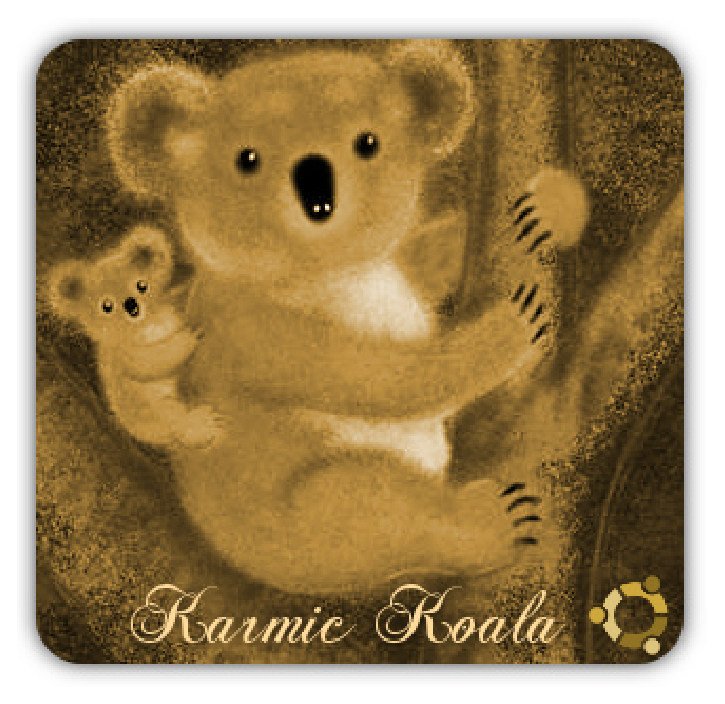
\includegraphics[height=8cm]{koala.eps}  
}\par

\bigskip
 
Et bien entendu\ldots

\bigskip

\includegraphics[width=10cm]{logo.epsi}

\end{center}

\normalsize

\vfill
\noindent
Autre logiciels utilisés : \href{http://fr.wikipedia.org/wiki/PSTricks}{pstricks} pour les figures, avec l'aide de \href{http://fr.wikipedia.org/wiki/Python_(langage)}{python} et \href{http://fr.wikipedia.org/wiki/SAGE_(logiciel_de_calcul_formel)}{Sage} pour la génération de certains bouts de code trop compliqués à programmer en \LaTeX.

\egroup

\normalsize



% This is part of Un soupçon de physique, sans être agressif pour autant
% Copyright (C) 2009-2010,2015
%   Laurent Claessens
% See the file fdl-1.3.txt for copying conditions.

\thispagestyle{empty}
\begin{center}
  \begin{minipage}{15cm}
    \hrule\par
    \vspace{2mm}
    \begin{center}
    \Huge \bfseries Un soupçon de physique  \par
    \Huge \bfseries sans être agressif pour autant \par
    \end{center}
    \hrule\par
  \end{minipage}
\end{center}

\vfill\vfill
\null\hfill Laurent \textsc{Claessens}\\
\null\hfill Dernière modification : \today\\
\null\hfill \url{http://student.ulb.ac.be/~lclaesse/}\\
\null\hfill \url{https://github.com/LaurentClaessens/echa}

\newpage

Copyright (c) 2006-2015  Laurent Claessens.

Permission is granted to copy, distribute and/or modify this document under the terms of the GNU Free Documentation License, Version 1.3 or any later version published by the Free Software Foundation; with no Invariant Sections, no Front-Cover Texts, and no Back-Cover Texts. A copy of the license is included in the section entitled ``GNU Free Documentation License''.

\vspace{1cm}

Si vous n'avez pas envie de lire toute la licence (ce que je comprends), en voici un mini résumé :
\begin{itemize}
	\item 
		Si vous donnez un pdf du document ou d'une partie à quelqu'un, vous \emph{devez} lui dire en même temps où il peut télécharger les sources \LaTeX. En pratique, le site sur lequel j'ai mit les sources actuelles est déjà indiqué sur la page de garde. Il n'y a donc rien à faire.
	\item
		Si vous modifiez le document, les nouvelles sources \LaTeX\ \emph{doivent} être publiées sur internet à une adresse publiquement accessible\footnote{Les zones de icampus protégées par un mot de passe ne sont pas valables; la dropbox non plus.}, et le site où les sources se trouvent doit être indiqué dans le document.
	\item
		En cas de modification, vous pouvez ajouter votre nom à la liste des auteurs des fichiers modifiés, mais vous ne pouvez pas retirer les noms déjà existants, de plus les modifications elles-mêmes doivent être publiés sous la même licence, et les sources \LaTeX\ des modifications doivent également être publiquement accessibles.
\end{itemize}

\vspace{1cm}

Le but principal de ces conditions est d'éviter que le document deviennent inutilisable parce que les sources \LaTeX\ seront perdues dans $5$ ans. Cela arrive trop souvent. Il s'agit d'un échange : je donne gratuitement le droit de copier, modifier et redistribuer le document, mais en échange, vous devez prendre soin des sources, et transmettre ces droits aux personnes à qui vous distribuez des versions modifiées.

Vous n'êtes par contre absolument pas obligés de me tenir au courant des modifications que vous apportez, bien que cela soit souhaitable pour que chacun puisse profiter des améliorations de tous les autres.



% TODO : il faut refaire toutes les figures pour qu'on puisse directement compiler en pdf.
% TODO : une fois que les figures sont bien faites, il faut fusioner avec smath.

\tableofcontents

\chapter{Introduction}
	% This is part of Un soupçon de physique, sans être agressif pour autant
% Copyright (C) 2006-2010
%   Laurent Claessens
% See the file fdl-1.3.txt for copying conditions.

\section{Matériel utilisé}

%---------------------------------------------------------------------------------------------------------------------------
\subsection{Logiciels}
%---------------------------------------------------------------------------------------------------------------------------

\begin{enumerate}
	\item
		Linux, Ubuntu Lucid
	\item
		\sout{Emacs et Gnome} Vim et KDE
	\item
		\AmS-\LaTeX
	\item
		\href{www.sagemath.org}{Sage} pour beaucoup de calculs, la préparation de graphiques, et pour les dernières figures.
	\item 
		\href{http://maxima.sourceforge.net/}{wxMaxima} avant que je ne découvre Sage.
	\item 
		\href{http://fr.wikipedia.org/wiki/PSTricks}{pstricks} pour les figures,
	\item
		\href{http://fr.wikipedia.org/wiki/Python_(langage)}{python} et \href{http://student.ulb.ac.be/~lclaesse/phystricks-doc.pdf}{phystricks} pour la programmation et les figures.
	\item
		Git et \href{www.gitorious.org}{gitorious} pour le partage des sources.
\end{enumerate}
Je tiens à en remercier tous les développeurs.
		
%---------------------------------------------------------------------------------------------------------------------------
\subsection{Sources}
%---------------------------------------------------------------------------------------------------------------------------

\begin{itemize}
	\item
		Le cours \emph{Mécanique et énergie} du \og site de la famille GG\fg. \href{www.cvgg.org}{www.cvgg.org}.
	\item 
		\href{http://gconnan.free.fr/}{Le site de Guillaume Connan}\footnote{À qui j'aurais pu téléphoner, mais\ldots}, et les questions pas toujours idiotes que Tehessin le rezeen y pose à son ô maître Mathémator. Bourré d'humour et d'excellentes explications mathématiques. La mad tea party de la page \pageref{PgMadTeaParty} en est l'emprunt le plus direct.
	\item 
		Le forum usenet de physique\footnote{\href{http://groups.google.fr/group/fr.sci.physique/topics?hl=fr.}{http://groups.google.fr/group/fr.sci.physique/topics?hl=fr.}} pour la linéarité des transformations de Lorentz et une fructueuse discussion sur la maximalité de la vitesse de la lumière. 
	\item 
		Wikipédia pour des liens hypertexte et pour le second degré.
	\item 
		Des discutions avec diverses personnes ayant lu des parties du texte.
	\item 
		les questions de mes élèves particuliers,\ldots
	\item 
		\ldots des idées glanées par-ci par-là dans les cours ---parfois très bien faits--- de leurs profs. Que ceux qui se sentent visés soient remerciés de mettre des cours de qualité entre les mains des enfants; qu'ils soient consolés que lesdits élèves parviennent encore à se faire morfler et à avoir besoin de cours particuliers; et qu'ils n'hésitent pas à poster sur \href{http://www.enseignons.be/}{http://www.enseignons.be/}.
\end{itemize}

Je m'en voudrais de ne pas citer le cours de math libre sesamath\footnote{\href{http://manuel.sesamath.net/}{http://sesamath.net/}}, dont je ne me suis pas inspiré de façon directe, mais qui peut quand même intéresser la lectrice de ces lignes.


%+++++++++++++++++++++++++++++++++++++++++++++++++++++++++++++++++++++++++++++++++++++++++++++++++++++++++++++++++++++++++++
					\section{Un cours de physique libre}
%+++++++++++++++++++++++++++++++++++++++++++++++++++++++++++++++++++++++++++++++++++++++++++++++++++++++++++++++++++++++++++

Ces notes ainsi que les sources \LaTeX{} sont librement publiées sur internet, cela signifie entre autres que chaque lectrice ou lecteur a le droit par tous les moyens de copier, modifier et redistribuer tout ou une partie du texte. En cela, je voudrais utiliser la puissance de l'internet pour mettre à portée de toutes et tous certaines connaissances en physique trop souvent confinées dans des manuels scolaires forts coûteux. J'espère qu'à l'avenir, la publication de texte libres d'enseignements fera à substantiellement baisser le prix de la scolarité.

Le partage est ce qu'on a trouvé de mieux pour propager la connaissance. De nombreuses autres initiatives internautes suivent cette idée. Citons Linux\footnote{\href{www.ubuntu.org}{www.ubuntu.org}} (qui fournit des tonnes de logiciels dans un esprit de liberté), l'encyclopédie libre Wikipedia\footnote{\href{www.wikipedia.org}{www.wikipedia.org}} et le (moins connu mais non moins intéressant) projet mutopia\footnote{\href{www.mutopiaproject.org}{www.mutopiaproject.org}} qui a pour ambition de publier sous format électronique et libre des partitions musicales tombées dans le domaine public (avis aux fans de musique). La plupart des sources données plus haut sont également publiées dans un esprit de partage libre.


%+++++++++++++++++++++++++++++++++++++++++++++++++++++++++++++++++++++++++++++++++++++++++++++++++++++++++++++++++++++++++++
					\section{Originalité de ce texte}
%+++++++++++++++++++++++++++++++++++++++++++++++++++++++++++++++++++++++++++++++++++++++++++++++++++++++++++++++++++++++++++

Le peu d'expérience de l'enseignement dont l'auteur de ces lignes peut se vanter sont trois cessions d'août d'Échec à l'echec et un bon nombre de cours particuliers, presque toujours entre la quatrième et la sixième secondaire. Les moments qui font plaisir, c'est quand un élève dit \og eh bien ! en fait c'est pas n'importe quoi la physique, maintenant que je comprends comment ça marche c'est chouette \fg.
   
J'ai donc développé une série de théories personnelles sur la façon dont il faudrait enseigner la physique et la mathématique. Je me suis donc mit à taper à l'ordinateur les mots que j'aurais dit si j'avais à expliquer oralement.

Parmi mes idées sur l'enseignement de la physique, celles qui diffèrent des cours \og traditionnels\fg{} sont plus ou moins celles-ci :
\begin{itemize}
\item je donne une préférence aux mots plutôt qu'aux formules : il ne s'agit pas de retenir que $P=F/S$, mais que \og Pression égal force divisé par surface\fg.
\item des exemples, des exemples, des exemples et encore des exemples, (sur ce point je ne suis pas encore du tout satisfait de mon résultat)
\item de l'humour, c'est marrant et ça détend l'atmosphère,
\item une définition peut avoir deux utilités : l'utilité première est d'être sûr que deux personnes parlent de la même chose quand elles utilisent le même mot; la seconde est d'avoir une correspondance entre les objets physiques étudiés et les objets mathématiques précis qui les décrivent. Je ne comprends pas pourquoi on assomme les enfants avec des définitions compliquées. Pourquoi définir une \og mesure\fg{} comme une \og comparaison avec une grandeur de même nature choisie arbitrairement comme étalon\fg ? Je suis sûr que la moitié des élèves qui connaissent cette définition n'ont pas été voir \emph{étalon} au dictionnaire.
\item De la rigueur mathématique. Ça ne fait pas de mal de faire remarquer que la vitesse se trouve en dérivant la position, et que bien souvent les conditions d'existences qui arrivent dans les résolutions d'équations décrivent des situations où la physique même du problème devient absurde. (vitesse infinie, bille qui roule sur un plan vertical). Un honnête personne de nos jours doit au moins une fois dans sa vie avoir entendu que la mathématique a une capacité à décrire la nature qui demeure au bas-mot étonnante.
\item Il y a je crois une grande différence entre la pédagogie de la mathématique et celle de la physique : en mathématique quand on remplace les lettres par des chiffres on comprend mieux. Si on ne comprend pas que $ax=b\Rightarrow x=b/a$, on peut regarder avec des nombres : $5\cdot 2=10\Rightarrow 2=10/5$, et on comprend mieux. En physique ce n'est pas vrai. Je ne crois pas qu'on comprend mieux la physique de ce qu'il se passe dans un exercice quand on remplace systématiquement toutes les lettres par les données de l'énoncé. Au contraire : le fond de la physique se trouve dans la manière dont les différentes grandeurs physiques se combinent (ou se simplifient !) dans les équations. Toute cette dynamique se perd quand on écrit des nombres à la place des lettres.
\item La physique est une science vivante. Il reste de nombreuses questions ouvertes. Certaines peuvent être énoncées sans connaissances très pointues, comme par exemple la miraculeuse coïncidence entre la masse dans la formule d'inertie $F=ma$ et la \emph{même} masse qui intervient dans la formule de l'énergie potentielle de gravitation $E=mgh$. La gravitation est liée à l'inertie d'une façon que personne ne comprend bien. Il y a un prix Nobel à prendre sur la question. Comme disait mon prof de relativité : \og En relativité générale, on postule l'égalité de la masse inertielle avec la masse pesante; mais c'est pas pour ça qu'on comprend mieux\fg.
\end{itemize}
Je crois pouvoir dire que dans le cadre de cours particuliers, ce petit programme a souvent été efficace. J'ai bien entendu eut des élèves qui sont restés indifférents à la physique et qui se sont contentés de réussir leur examen dans l'apparente ignorance de la beauté de la chose. Mais j'ai également eut des élèves qui ont finit par accepter que c'est amusant de réfléchir à un problème de physique quand on comprend ce qu'il veut dire.

Ici, ce sont des notes écrites dans lesquelles j'ai essayé de remettre ce que j'ai dit à différents élèves. On verra.

\section{Rappels}
%++++++++++++++++

\subsection*{Conseils de travail}
%----------------------------


\begin{enumerate}
\item Convertis les unités donnés en unités SI. 
\item Fais des scraboutchas, des oeuvres, des schémas, gribouilles, ce que tu veux mais dessines !
    Comme tu le vois, ce manuel contient un certain nombre de dessins. Ils ne sont pas faits pour être regardés avec admiration béate; ils sont faits pour inspirer les dessins que tu feras sur ta feuille. Tu dois comprendre le sens des dessins et être capable de les réinventer.
\item Si on te parle d'un triangle quelconque, n'en dessine pas un équilatéral, isocèle ou rectangle.
\item Écris de phrases complètes sur ton papier de brouillon. N'écris pas \og $R_c=3$ et $v_A=10$ \fg{} mais \og Le rayon du cylindre est \unit{3}{\meter} et la vitesse de $A$ est \unit{10}{\meter\per\second}\fg.


En particulier, méfies toi des \og formules\fg{} toute faites. Le symbole $F$ peut très bien désigner,  d'après le contexte,  une force quelconque ou un frottement; tout comme $P$ peut désigner la pesanteur, la pression ou la puissance. Ces symboles peuvent donc arriver dans plusieurs formules qui ne peuvent absolument pas être comparée. Donc il vaut toujours mieux un long discours qu'une petite formule. 

Tu dois pouvoir donner avec des mots la signification de tous les symboles que tu écris.


\item On n'efface pas une faute : on la barre proprement. Quand tu étudieras, il est tout aussi important de \emph{comprendre} les fautes que tu as faites que de comprendre les réponses justes. Si tu ne comprends pas pourquoi tu as fais une faute une fois, tu referas la faute.
\item Dans le même ordre d'idée, exit les correcteurs et tip-ex : quelque chose que tu crois faux pendant 10 secondes peut très bien être vrai. Ce serait bête de perdre l'idée pour quelque instants de doute.
\item Quand tu as la réponse, prends une feuille blanche, et récris \emph{proprement et à fond} toutes les étapes du raisonnement
\end{enumerate}

Ce n'est pas au moment où tu peux dire par coeur une définition que tu  \emph{connais} la définition. La physique est une science qui étudie la réalité; l'étude des mots compliqués qui rentrent dans une définition est du ressort de la \href{http://fr.wikipedia.org/wiki/Lexicologie}{lexicographique} ou de la \href{http://fr.wikipedia.org/wiki/Sémantique}{sémantique} et n'a aucun intérêt ici.

Pour voir si tu as compris une définition, tu dois pouvoir donner des exemple avec de préférence des objets que tu as sous les yeux au moment où tu lis la théorie -- dans ta chambre, dans ta classe, sur ton lit ou dans ta douche. Tu dois également être capable d'expliquer pourquoi tel ou tel exemple rentre bien dans la définition donnée.

\subsection{Avertissement}
%-------------------------

J'essayerai de ne faire aucun effort pour avoir une notation constante dans le texte. Les distances seront parfois notées $l$ (comme longueur), parfois $d$ (comme distance), la force de pesanteur sera notée indifféremment $ \fG$ (comme gravitation) ou $\fP$ (comme pesanteur) à ne pas confondre avec le $P$ de la puissance ou celui de la pression. Pourquoi ? Parce que je ne veux pas que tu retiennes des formules sous forme analytique : pas question de retenir $G=mg$ ou $W=Fd$. Il faut retenir
\begin{center}
force de gravitation sur un objet $=$ masse de l'objet fois constante $g$,
\end{center}
et
\begin{center}
travail d'une force qui bouge $=$ grandeur de la force fois le déplacement.
\end{center}


\subsection{Du système international}
%------------------------------------

Les unités se répartissent en trois catégories : les unités \emph{de base} du système international (SI), les unités \emph{dérivées} et les unités \emph{hors SI}. Affin d'éviter les erreurs de calcul, il est \emph{hyper-important} (!!) de n'utiliser que les unités du SI et ses dérivées.


\subsubsection{Les unités de base}
\begin{description}
\item[masse] kilogramme, noté \kilogram 
\item[longueur] mètre, noté \meter
\item[temps] seconde, noté \second
\item[courant électrique] ampère, noté \ampere.
\end{description}
\subsubsection{Les unités dérivées}
Ce sont toutes les unités qu'on peut obtenir en multipliant ou divisant les unités fondamentales entre-elles. Les plus courantes sont données dans le tableau \ref{TabUnitsSI}.

\begin{table}[hc]
\centering
\begin{tabular}{lccc}
Quantité & Unité & Abréviation & Conversion\\
\hline
Force              & newton  & \newton  & \kilogram\usk\meter\per\second\squared \\
Énergie et travail & joule   & \joule  & \kilogram\usk\meter\squared\per\second\squared\\
Puissance          & watt    & \watt  &  \kilogram\usk\meter\squared\per\cubic\second\\
Pression           & pascal  & \pascal & \kilogram\per\meter\usk\square\second\\
Fréquence          & hertz   & \hertz & $\reciprocal\second$
\end{tabular}
\caption{Les unités les plus courantes qui sont valables dans le système international.}\label{TabUnitsSI}
\end{table}

Toutes les autres unités sont à proscrire et à convertir avant de commencer quoi que ce soit.

\begin{description}
\item[longueurs] centimètres, kilomètres, années-lumière,\ldots $\rightarrow$ mètres
\item[temps] jours, années, minutes, heures,\ldots $\rightarrow$ secondes
\item[vitesses] kilomètres/heures\ldots $\rightarrow$ mètres/seconde
\end{description}

\begin{exemple}
Un exemple où on a l'impression que ce blabla ne sert à rien : un train avance à \unit{240}{\kilo\meter\per\hour} pendant une heure et demi. On multiplie 240 par 1,5 et on trouve bien que la distance parcourue est \unit{360}{\kilo\meter}. 

Pour bien faire, on devrait convertir $\unit{120}{\kilo\meter\per\hour}= \unit{33.333}\meter\per\second$ et $\unit{1.5}{\hour}=\unit{5400}{\second}$ puis multiplier pour trouver \unit{180000}{\meter}, qui est effectivement la même chose que \unit{180}{\kilo\meter}, mais obtenu de façon plus compliquée.
\end{exemple}

\begin{exemple}
Un exemple où l'on remarque que c'est important : une pierre est en chute libre pendant 2 minutes. Pour trouver la distance parcourue, on fait $gt^2/2$ avec $t=2$ et $g=9,81$. On trouve 19.62. Et c'est faux. Pourquoi ? Parce que quand on prend la peine d'écrire les unités, on remarque que $g=\unit{9.81}{\underline{\meter\per\square\second}}$. Dire \og $g=9.81$\fg, ça présuppose donc déjà un choix d'unité !

En fait à chaque fois qu'on utilise une constante physique \og qu'on connaît par coeur\fg{} sans convertir les données en système SI, on va droit dans le panneau.
\end{exemple}

\subsection{Le point matériel}
%------------------------------


Un corps matériel occupe un volume et possède une masse. Souvent, le volume occupé est petit par rapport au volume ambiant. Par exemple si on dit que la maison de la schtroumfette est à \unit{25}{\meter} ce celle du grand schtroumpf, on fait \og comme si\fg{} les deux maisons étaient des points dans le village; il est en effet possible que la penderie de bonnets rouges du grand schtroumf soit à \unit{24}{\meter} de la porte d'entrée de la schtroumfette ou que le PC de la schtroumfette soit à \unit{27}{\meter} de la réserve secrète d'alcools du grand schtroumpf. Quoi qu'il en soit, la plupart du temps,  on décrit la position des maisons avec des espèces de moyennes sans tenir compte de la structure interne des maisons.

Autre exemple : la croix sur la carte au trésor indique juste un point de l'île, sans préciser si ce point est le coin arrière gauche ou avant droit du coffre. Le pirate a fait comme si le coffre était juste un point. À moins que le butin soit vraiment énorme ou que l'île soit minuscule, le trésor est bien un point par rapport à l'ensemble de l'île.

\begin{definition}
Lorsque un objet est petit par rapport à l'espace dans lequel il se déplace, nous faisons souvent comme si il se réduisait à un seul point. Cette approximation est ce que nous appelons l'hypothèse du \defe{point matériel}{Point matériel}. 
\end{definition}

Dans les problèmes où la masse de l'objet est importante, le point que l'on confond avec l'objet complet est le \emph{centre de gravité} du corps matériel.


\begin{exemple}
Les objets suivants peuvent être considérés comme des points matériels.
\begin{enumerate}
\item Un vélo qui se déplace entre Pékin et Madrid
\item un ballon sur un terrain de football,
\item la lune autour de la terre,
\item une mouche dans la cuisine.
\end{enumerate}
\end{exemple}

\begin{exercice}
Donnez d'autres exemples de point matériel. Donnez aussi quelque exemples de choses qui ne sont pas des points matériels, comme le blanc dans un oeuf, par exemple. Donnez en particulier une situation dans laquelle une rame de métro n'est pas un point matériel.
\end{exercice}



\chapter{Principes généraux de la physique}
	% This is part of Un soupçon de physique, sans être agressif pour autant
% Copyright (C) 2006-2009
%   Laurent Claessens
% See the file fdl-1.3.txt for copying conditions.




	% This is part of Un soupçon de physique, sans être agressif pour autant
% Copyright (C) 2006-2009
%   Laurent Claessens
% See the file fdl-1.3.txt for copying conditions.


Ce chapitre a pour objectif de parler de quelque principes généraux de la physique qui transcendent l'une ou l'autre matière précise.

\section{Homogénéité et isotropie}
%+++++++++++++++++++++++++++++++++

\subsection{Homogénéité de l'espace}
%-----------------------------------

En physique, nous supposons que l'espace est homogène, c'est à dire qu'il n'y a pas un lieu privilégié. Voici deux façons de se représenter ce principe :
\begin{itemize}
\item Il n'y a pas un endroit dans l'univers où un panneau est planté pour dire \og ici c'est l'endroit de référence\fg,
\item si on fait la même expérience à deux endroits différents, on doit obtenir le même résultat.
\end{itemize}


Ce principe n'est évidement correct que si \emph{tous} les paramètres de l'expérience sont reproduits. Si mon expérience est de voir à quelle température l'eau entre en ébullition, j'aurai un résultat différent ici ou au sommet de l'Éverest (pour des questions de pression). Mais si je me mets ici dans un caisson à la pression du sommet de l'Éverest, je trouverai le bon résultat.

Une importante conséquence de ce principe est le fait que si une expérience dépend de la position de deux points, en fait le résultat ne peut dépendre que de la \emph{différence} entre les deux points, et non de leur position exacte dans l'espace. L'exemple le plus simple est de mettre par exemple deux aimants en présence. Ils vont s'attirer avec une certaine force. Je ne sais pas cette force, mais je sais que si le premier aimant est à la position $\overrightarrow{ r }$ et le second à la position $\overrightarrow{ r }+ \overrightarrow{ a }$, cette force ne dépendra que de $\overrightarrow{ a }$, c'est à dire de la position relative de l'un par rapport à l'autre, mais pas de leur position absolue dans l'espace.

\subsection{Homogénéité du temps}
%--------------------------------

Prenons un exemple. Tu veux étudier un pendule. Tu lance ton chrono quand tu rentre dans le labo, tu marche à ton aise vers le pendule, tu prends l'extrémité du pendule, tu la déplace un peu. Au moment de lâcher, tu regardes où en es ton chrono. Tu notes le résultat : une minute et vingt cinq secondes. Le pendule fait un aller-retour. Au moment où il a fini, tu regardes à nouveau ton chrono et tu notes le résultat : une minute et vingt sept secondes.

Le principe d'homogénéité te dit que toutes les caractéristiques mesurables du pendules sont contenues dans les \emph{différences} de temps. En l'occurrence, la période du pendule sera la différence entre une minute vingt sept et une minute vingt cinq, soit deux secondes.

En particulier, l'opération de \emph{somme} entre tes deux mesures n'a pas de sens : la grandeur de deux minutes et cinquante deux secondes n'a aucun rapport avec le pendule !

Si tu refais l'expérience le lendemain, tu lâches le pendule à vingt six heures, trente sept minutes et quatorze secondes; et une période plus tard, on en est à vingt six heures, trente sept minutes et seize secondes. À nouveau c'est la différence de deux secondes entre les deux mesures qui a un sens physique.

\subsection{Conclusion des homogénéités}		\label{SecConcHomo}
%------------------------------------

Si dans un système de coordonnées spatio-temporel, tu étudies un phénomène en mesurant deux événements intervenant dans le phénomène aux endroits et instants $(t_0,x_0)$ et $(t_1,x_1)$, les seules grandeurs qui caractérisent réellement le phénomène sont la durée $t_1-t_0$ et la distance $x_1-x_0$.

\subsection{Isotropie de l'espace}
%---------------------------------


\section{Le principe de relativité}
%+++++++++++++++++++++++++++++++++++

%http://fr.wikipedia.org/wiki/Théorie_de_la_relativité
Le \href{http://fr.wikipedia.org/wiki/Théorie_de_la_relativité}{principe de relativité} est un des plus vieux principes physique : il remonte à \href{http://fr.wikipedia.org/wiki/Relativité_galiléenne}{Galilée}. Son contenu est assez simple.
\begin{loiphyz}
Les lois de la nature sont les mêmes dans tous les référentiels d'inertie. En d'autres termes, si vous êtes dans une pièce fermée, il n'existe aucune expérience qui vous permet de savoir si vous êtes au repos ou en mouvement rectiligne uniforme.
\end{loiphyz}

Une conséquence remarquable de ce principe est qu'il est possible de jongler dans le métro entre deux stations. En effet, tant que le métro avance à une vitesse constante, tout se passe exactement comme si il était à l'arrêt, et les balles se comporteront exactement comme dans ton salon.

Autre conséquence. Un principe général en science\footnote{En sciences, j'entends en \emph{vraies} sciences; exit l'astrologie, la philosophie, la graphologie, la psychologie, les sciences politiques, la sorcellerie et autres charlatanismes.} est que si il n'existe pas d'expériences pour distinguer deux choses alors les deux choses doivent être considérées comme équivalentes. Par conséquent, on ne peut pas définir de \emph{repos absolu} parce qu'il serait impossible à distinguer du mouvement rectiligne uniforme. Toute personne se déplaçant en MRU a le droit de se considérer au repos et de dire que c'est le reste de l'univers qui se déplace.




\chapter{Optique géométrique}
	% This is part of Un soupçon de physique, sans être agressif pour autant
% Copyright (C) 2006-2009
%   Laurent Claessens
% See the file fdl-1.3.txt for copying conditions.


\section*{Introduction : propagation de la lumière}
%----------------------------------

Tu remarqueras qu'une bonne lampe de poche envoie de la lumière dans une seule direction. On parle de \defe{faisceau de lumière}{}. Et pourtant tu sais bien que l'ampoule éclaire dans tous les sens. Ce qu'il se passe est qu'une ampoule envoie des rayons dans tous les sens, mais qu'une lampe de poche est munie d'un système pour dévier les rayons qui ne vont pas dans le bon sens, de telle manière à ce que, au final, la lampe de poche émette un faisceau lumineux.

Nous allons considérer que la lumière se compose de \defe{rayon lumineux}{} : elle se propage en ligne droite. 

Un faisceau est composé de plusieurs rayons (disons au moins des millions par centimètre carré) qui peuvent être parallèles, divergents ou convergents.

\newcommand{\prefigoptfaisc}{%
\pstGeonode(0,-0.3){dA}(3,-0.3){fA}
\pstGeonode(0,0){dB}(3,0){fB}
\pstGeonode(0,0.3){dC}(3,0.3){fC}
}

\begin{figure}[ht]
\centering
\subfigure[Rayons parallèles. Exemple : les rayons solaires]{%
\begin{pspicture}(-0.5,-0.5)(4.5,0.5)
	\psset{PointSymbol=none, PointName=none}
	\prefigoptfaisc
	\pstRayon{dA}{fA}
	\pstRayon{dB}{fB}
	\pstRayon{dC}{fC}
\end{pspicture}
}						% Fermeture de la sous-figure
\subfigure[Rayons divergents. Exemple : n'importe quelle lumière électrique]{%

\begin{pspicture}(-0.5,-0.5)(4.5,0.5)
	\psset{PointSymbol=none, PointName=none}
	\prefigoptfaisc
	\pstRayon{dB}{fA}
	\pstRayon{dB}{fB}
	\pstRayon{dB}{fC}
\end{pspicture}
}
\subfigure[Rayons convergents. Pour en obtenir, on utilise une loupe, voir section \ref{SecLentMinces}.]{%
\begin{pspicture}(-0.5,-0.5)(4.5,0.5)
	\psset{PointSymbol=none, PointName=none}
	\prefigoptfaisc
	\pstRayon{dA}{fB}
	\pstRayon{dB}{fB}
	\pstRayon{dC}{fB}
\end{pspicture}
}						% Fermeture de la sous-figure

\caption{Dispositions possibles des rayons lumineux dans un faisceau}
\end{figure}
%http://fr.wikipedia.org/wiki/Optique_géométrique
%http://fr.wikipedia.org/wiki/Optique_quantique
%http://fr.wikipedia.org/wiki/Optique_ondulatoire
%http://fr.wikipedia.org/wiki/Optiquen
La théorie de la lumière basée sur l'idée que la lumière suit des rayons rectiligne est baptisée l'\href{http://fr.wikipedia.org/wiki/Optique_géométrique}{\defe{optique géométrique}{}} parce que la majorité des raisonnements et des résultats s'obtiennent en calculant des angles et des intersections sur des figures géométriques. 

L'optique géométrique n'est qu'une toute petite partie de \href{http://fr.wikipedia.org/wiki/Optique}{l'optique}. Tu verras peut-être plus tard une description plus précise des phénomènes lumineux en \href{http://fr.wikipedia.org/wiki/Optique_ondulatoire}{optique ondulatoire}. Si tu manges vraiment beaucoup de soupe, et que tu choisis de faire des études poussées en physique, tu verras l'arme absolue des théories de la lumière : \href{http://fr.wikipedia.org/wiki/Optique_quantique}{l'optique quantique}. Ceci pour dire que ce dont on va parler ici n'est pas du tout le dernier mot de l'histoire\ldots Ce cours concerne des choses qui sont essentiellement connues depuis les dix-sept et dix-huitième siècle ! 

\section{Réflexion et réfraction de la lumière}
%+++++++++++++++++++++++++++++++++++++++++++++++

\subsection{Réflexion et réfraction}
%-----------------------------------
%http://fr.wikipedia.org/wiki/Réflexion_optique
%http://fr.wikipedia.org/wiki/Réfraction

Considère deux milieux transparents (air, plastique transparent, verre ou eau), et envoie un rayon lumineux oblique de l'un vers l'autre. Prend par exemple une latte en plastique et capte un rayon de Soleil avec. Tu sais qu'une partie de la lumière subit une \href{http://fr.wikipedia.org/wiki/Réflexion_optique}{\defe{réflexion}{}} : c'est pour ça que tu peux t'amuser à éblouir les gens en envoyant le rayon réfléchi sur leurs yeux.

Mais tu sais aussi que cette réflexion ne rend pas le plastique opaque pour autant : une partie de la lumière rentre dans le plastique (et en ressort, mais c'est une autre histoire). La partie de la lumière qui rentre dans le plastique est dite \href{http://fr.wikipedia.org/wiki/Réfraction}{\defe{réfractée}{}} 

Il se fait que le rayon réfracté (la partie qui rentre dans le plastique, dans l'eau ou le verre) est déviée au passage. Cela ne se voit pas très bien dans le cas de la lumière solaire captée par la latte en plastique, mais cela se voit par contre très bien quand tu plonge un bout de bois dans de l'eau : à l'endroit où il entre dans l'eau, il semble cassé. Le rayon provenant du bâton sort de l'eau avec une \og déviation\fg). Ceci est montré sur la figure \ref{fig_refr_pm}.

\newcommand{\prefigoptdifr}{%

	\psset{PointSymbol=none, PointName=none}
\pstGeonode(0,0){O}(2,0){P}
\pstRotation[RotAngle=90]{O}{P}[Qi]
\pstHomO[HomCoef=0.5]{O}{Qi}[Q]
\pstRotation[RotAngle=180]{O}{P}[R]
\pstHomO[HomCoef=-1]{O}{Q}[S]
\pstRotation[RotAngle=-20]{O}{R}[Ri]		% Je place le rayon incident avec un certain angle avec le plan
    \pstDioptre{O}{P}{Ri}{0.9}{2}{Rs}{Re}	% La passage par le dioptre
}

\begin{figure}[ht]
\centering
\begin{pspicture}(-2,-2)(2,1)
	\prefigoptdifr
 %\psframe[linecolor=blue](-2,-2)(2,1)

   \pstRayon{Ri}{O}
   \pstRayon{O}{Re}
   \pstRayon{O}{Rs}

   \psline(R)(P)
   \psline[linecolor=lightgray](O)(Q)
   \psline[linecolor=lightgray](O)(S)

\end{pspicture}
\caption{Réflexion et réfraction d'un rayon lumineux qui passe d'un milieu moins réfringent à plus réfringent}\label{fig_refr_pm}
\end{figure}

Avec certaines surfaces, presque tous les rayons lumineux sont réfléchis, et seule une petite partie est absorbée. Dans ce cas, il n'y a quasiment pas de rayon réfracté, et on a alors un miroir.

\subsection{La réflexion}
%------------------------

Étudions plus spécifiquement le rayon réfléchi. Assez logiquement, le rayon incident va simplement \og faire ricochet\fg{} sur la surface, et donc repartir avec un angle égal à l'angle d'arrivée, d'où les deux lois suivantes :

\begin{loiphyz}
Les rayons incidents et réfléchis sont dans un même plan perpendiculaire à la surface. Ce plan est appelé le \emph{plan d'incidence}.
\end{loiphyz}

\begin{loiphyz}
L'angle d'incidence est égal à l'angle de réflexion $\hat \imath=\hat r$.
\end{loiphyz}

Nous allons donner une preuve de ces deux lois dans la sous section \ref{SubsecSnellVitesse} en utilisant un petit peu d'optique ondulatoire. L'important est de retenir que ces deux lois ne sont pas \og évidentes\fg{} en soi, mais sont la partie émergée de l'iceberg qu'est le comportement ondulatoire de la lumière. Une description complète du phénomène demande de voir la lumière comme une onde électromagnétique. Cela devient vite très compliqué.


\newcommand{\prefigreflexion}[1]{%

\pstGeonode(0,0){O}(2,0){P}
\pstRotation[RotAngle=90]{O}{P}[Qi]
\pstHomO[HomCoef=0.5]{O}{Qi}[Q]
\pstRotation[RotAngle=180]{O}{P}[R]
\pstHomO[HomCoef=-1]{O}{Q}[S]
\pstRotation[RotAngle=-#1]{O}{R}[Ri]		% Je place le rayon incident avec un certain angle avec le plan
    \pstDioptre{O}{P}{Ri}{0.9}{2}{Rs}{Re}	% La passage par le dioptre
}

\newcommand{\tracefigreflexion}{%

   \pstMarkAngle{Q}{O}{Ri}{$\hat\imath$}
   \pstMarkAngle{Rs}{O}{Q}{$\hat r$}

   \psline(R)(P)
   \psline[linecolor=lightgray](O)(Q)
   \psline[linecolor=lightgray](O)(S)

   \pstRayon{Ri}{O}
   \pstRayon{O}{Rs}
}

\begin{figure}[ht]
\centering

\subfigure{%
\begin{pspicture}(-2,-1)(2,1.5)
	\psset{PointSymbol=none, PointName=none}
	\prefigreflexion{10}
	\tracefigreflexion
\end{pspicture}
}						% Fermeture de la sous-figure
%
\subfigure{%
\begin{pspicture}(-2,-1)(2,1.5)
	\psset{PointSymbol=none, PointName=none}
	\prefigreflexion{20}
	\tracefigreflexion
\end{pspicture}
}						% Fermeture de la sous-figure
%
\subfigure{%
\begin{pspicture}(-2,-1)(2,1.5)
	\psset{PointSymbol=none, PointName=none}
	\prefigreflexion{40}
	\tracefigreflexion
\end{pspicture}
}						% Fermeture de la sous-figure
%
\subfigure{%
\begin{pspicture}(-2,-1)(2,1.5)
	\psset{PointSymbol=none, PointName=none}
	\prefigreflexion{60}
	\tracefigreflexion
\end{pspicture}
}						% Fermeture de la sous-figure
%
\subfigure{%
\begin{pspicture}(-2,-1)(2,1.5)
	\psset{PointSymbol=none, PointName=none}
	\prefigreflexion{90}
	\tracefigreflexion
\end{pspicture}
}						% Fermeture de la sous-figure
%
\subfigure{%
\begin{pspicture}(-2,-1)(2,1.5)
	\psset{PointSymbol=none, PointName=none}
	\prefigreflexion{120}
	\tracefigreflexion
\end{pspicture}
}						% Fermeture de la sous-figure
%
\caption{Divers rayons réfléchis}\label{fig_reflexion}
\end{figure}


On parle de temps en temps d'une troisième loi qui a au moins le mérite d'avoir un nom marrant; je te laisse juger. 

\begin{loiphyz}[Loi du retour inverse]
Les lois de la réflexion sont indépendantes du sens de parcours de la lumière.
\end{loiphyz}
 
Cette loi n'en n'est cependant pas une parce qu'elle peut se déduire des deux premières, comme montré sur la figure \ref{fig_retourinverse}.

\newcommand{\prefigretourinverse}{%
			
\pstGeonode(0,0){O}(2,0){P}
\pstRotation[RotAngle=90]{O}{P}[Qi]
\pstHomO[HomCoef=0.5]{O}{Qi}[Q]
\pstRotation[RotAngle=180]{O}{P}[R]
\pstHomO[HomCoef=-1]{O}{Q}[S]
\pstRotation[RotAngle=-40]{O}{R}[Ri]		% Je place le rayon incident avec un certain angle avec le plan
    \pstDioptre{O}{P}{Ri}{0.9}{2}{Rs}{Re}	% La passage par le dioptre
}

\begin{figure}[ht]
\centering
\subfigure[La situation habituelle \ldots]{%
\begin{pspicture}(-2,-1)(2,1.5)
	\psset{PointSymbol=none, PointName=none}
	\prefigretourinverse

   \pstRayon{Ri}{O}
   \pstRayon{O}{Rs}

   \pstMarkAngle{Q}{O}{Ri}{$\hat\imath$}
   \pstMarkAngle{Rs}{O}{Q}{$\hat r$}

   \psline(R)(P)
   \psline[linecolor=lightgray](O)(Q)
   \psline[linecolor=lightgray](O)(S)

\end{pspicture}
}						% Fermeture de la sous-figure
\subfigure[\ldots et quand on inverse les flèches]{%
\begin{pspicture}(-2,-1)(2,1.5)
	\psset{PointSymbol=none, PointName=none}

	\prefigretourinverse

   \pstRayon{O}{Ri}
   \pstRayon{Rs}{O}

   \pstMarkAngle{Q}{O}{Ri}{$\hat r$}
   \pstMarkAngle{Rs}{O}{Q}{$\hat \imath$}

   \psline(R)(P)
   \psline[linecolor=lightgray](O)(Q)
   \psline[linecolor=lightgray](O)(S)

\end{pspicture}

}						% Fermeture de la sous-figure
\caption{La loi du retour inverse : comme $\hat\imath=\hat r$, les deux dessins sont interchangeables et la loi du retour inverse est une évidence.}\label{fig_retourinverse}
\end{figure}

\subsection{La réfraction}
%-------------------------

Lorsque la lumière change de milieu, elle dévie. Pour t'en convaincre, prends un verre d'eau et enfonce ton crayon dedans (je ne rigole pas : fais-le !). Tu observes qu'au passage de l'air à l'eau, le crayon est comme \og cassé\fg. Je ne connais hélas pas de moyens simples pour prouver que les choses sont ainsi, mais c'est ainsi. Oublions un instant le rayon réfléchi, et regardons la figure \ref{fig_refraction}.


\newcommand{\prefigrefraction}{%
\pstGeonode(0,0){O}(2,0){P}
\pstRotation[RotAngle=90]{O}{P}[Qi]
\pstHomO[HomCoef=0.5]{O}{Qi}[Q]
\pstRotation[RotAngle=180]{O}{P}[R]
\pstHomO[HomCoef=-1]{O}{Q}[S]
\pstRotation[RotAngle=-20]{O}{R}[Ri]		% Je place le rayon incident avec un certain angle avec le plan
    \pstDioptre{O}{P}{Ri}{0.9}{2}{Rs}{Re}	% La passage par le dioptre
}

\begin{figure}[ht]
\centering
\begin{pspicture}(-2,-2.0)(2,1)
%\psframe[linecolor=green](-2,-2.0)(2,1)
	\psset{PointSymbol=none, PointName=none}
	\prefigrefraction

   \psline(R)(P)
   \psline[linecolor=lightgray](O)(Q)
   \psline[linecolor=lightgray](O)(S)

   \pstRayon{Ri}{O}
   \pstRayon{O}{Re}

   \pstMarkAngle{S}{O}{Re}{$\hat r$}
   \pstMarkAngle{Q}{O}{Ri}{$\hat\imath$}
\end{pspicture}
\caption{Un rayon lumineux est réfracté en entrant dans un verre d'eau}\label{fig_refraction}
\end{figure}

La réfraction obéit à deux lois.
%\setcounter{numloiphyz}{0}		% Note qu'il faudra souvent le remettre à zéro ce compteur. Genre à tous les coups.
\begin{loiphyz}
Les rayons incidents, réfléchis et réfractés sont dans un même plan, perpendiculaire à la surface. Ce plan est appelé le \emph{plan d'incidence}.
\end{loiphyz}


\begin{loiphyz}[Loi de  \href{http://fr.wikipedia.org/wiki/Snell}{Snell}- \href{http://fr.wikipedia.org/wiki/Descartes}{Descartes}]
L'angle d'incidence et de réfraction sont liés par la relation
\begin{equation}   \label{EqSinNDeuxUn}
\frac{ \sin\hat\imath }{ \sin\hat r }=n_{2/1}
\end{equation}
où $n_{2/1}$ est l'\defe{indice de réfraction}{} du milieu 2 par rapport au milieu 1. On l'appelle aussi l'indice de \defe{réfraction relatif}{}.
\end{loiphyz}
Exemples d'indices de réfraction relatifs :
\begin{itemize}
\item $n_{\text{verre/air}}=3/2$,
\item $n_{\text{diamant/air}}=2.42$,
\item $n_{\text{eau/air}}=4/3$.
\end{itemize}


	\subsection{Loi de Snell-Descartes et vitesse de la lumière}   \label{SubsecSnellVitesse}
%-----------------------------------------------------------

\paragraph{Avertissement}
La preuve apportée ici à la loi de Snell-Descartes utilise le fait que la lumière se comporte comme une onde. La notion de front d'onde sera utilisée. Le niveau est donc un peu plus élevé que d'habitude.

\paragraph{}

Le phénomène de réfraction est dû à une différence de vitesse de propagation de la lumière entre deux milieux. Prenons l'exemple de l'air et de l'eau. Dans l'air, la lumière parcours environ \unit{300\,000}{\kilo\meter\per\second}, tandis que dans l'eau cette vitesse n'est que de \unit{225\,000}{\kilo\meter\per\second}. 

Considérons un paquet de rayons de lunes parallèles qui arrivent à la surface d'un étang par une belle nuit étoilée. Tant que la lumière ne touche pas du tout l'eau, tous les rayons avancent ensemble, au moment où des rayons commencent à pénétrer dans l'eau, les choses commencent à se compliquer. Durant le temps entre le moment où le premier rayon entre dans l'eau et le moment où les deux autres y parviennent, le premier rayon avance moins vite que les deux suivants. On voit alors tout de suite que le tout ne va plus avancer en un bloc, mais se déformer.

Il est donc clair qu'il va se passer quelque chose. Pouvons-nous voir plus précisément ce qui va se passer ?

\begin{exercice}
Le rayon de la Terre vaut \unit{6500}{\kilo\meter} à l'équateur. Combien de tours de la Terre la lumière peut-elle faire en une seconde. Le Soleil se trouve à \unit{149\,600\,000}{\kilo\meter} de la Terre. Combien de temps mets la lumière solaire pour arriver jusqu'à nous ? 

Mars se trouve à \unit{227\,900\,000}{\kilo\meter} du Soleil. Quelle est la distance minimale que l'on peut espérer trouver entre la Terre et le Soleil ? Combien de temps il faut à la lumière pour aller de la Terre à Mars dans ces conditions ? Cela incite à la plus grande prudence quand on télécommande des robots sur Mars depuis la Terre, et peut poser des problèmes pratiques quant à l'organisation d'un tournois d'échecs interplanétaire.
\end{exercice}

\subsubsection{Physique de la réfraction}
%-------------------------------------

\newcommand{\prefigcalcrefr}{%
\pstGeonode(0,0){A}(2,0){B}			% Définition de la droite d'interface
\pstHomO[HomCoef=-1]{A}{B}[B']			
\pstHomO[HomCoef=2]{A}{B}[A']
\pstRotation[RotAngle=-50]{A}{B'}[r1]		% Angle d'incidence
\pstTransHom{A}{r1}{B}{1}{r2}
\pstRotation[RotAngle=90]{A}{r1}[pl]
\pstInterLL{A}{pl}{B}{r2}{C}
\pstTransHom{C}{B}{A}{0.5}{Cl}			% Vitesse de la lumière dans le milieu
\pstInterLC{B'}{A'}{A}{Cl}{C1}{C2}
%\pstInterCC{B}{A}{A}{Cl}{t1}{t2}
\pstTangenteOPM{A}{Cl}{B}{t2}{t1}
%\pstInterLL{A}{B}{pg}{qg}{m}			
%\pstTransHom{p}{pd}{p}{-1}{pg}			
%\pstRotation[RotAngle=90]{O}{P}[Qi]
%\pstRotation[RotAngle=180]{O}{P}[R]
%\pstHomO[HomCoef=-1]{O}{Q}[S]
%\pstRotation[RotAngle=-20]{O}{R}[Ri]		
%    \pstDioptre{O}{P}{Ri}{0.9}{2}{Rs}{Re}	
}

\begin{figure}[ht]
\centering

%\subfigure[Le tout]{%
%\begin{pspicture}(-2,-1)(4,2)
% \psframe[linecolor=blue](-2,-1)(4,2)
%	\psset{PointSymbol=none, PointName=none}
%	\prefigcalcrefr
%
%	\psline[linecolor=blue](B')(A')
%	\pstRayon{r1}{A}\pstRayon{r2}{B}
%	\psline(A)(C)
%	\pstArcOAB{A}{C1}{C2}
%	\psline(B)(t1)
%	\pstRayon{A}{t1}
%\label{letout}
%\end{pspicture}
%}
%
\subfigure[Le trait bleu pointillé représente le trajet que le rayon $B$ doit encore parcourir avant d'arriver sur l'interface au moment où le rayon $B$ vient d'y arriver]{%
\begin{pspicture}(-2,-1)(4,2)
% \psframe[linecolor=blue](-1,-1)(2,1)
	\psset{PointSymbol=none, PointName=none}
\prefigcalcrefr

	\psline(B')(A')
	\pstRayon{r1}{A}\pstRayon{r2}{C}
	\psline[linecolor=green](A)(C)
	\psline[linecolor=blue, linestyle=dashed](C)(B)
\label{lepremier}
\end{pspicture}
}
%
\subfigure[Où le rayon $A$ a-t-il pu aller durant ce temps ?]{%
\begin{pspicture}(-2,-1)(4,2)
% \psframe[linecolor=blue](-1,-1)(2,1)
	\psset{PointSymbol=none, PointName=none}
\prefigcalcrefr

	\psline(B')(A')
	\pstRayon{r1}{A}\pstRayon{r2}{B}
	\pstMarquePoint{B}{0.3;-90}{$Q$}
	\psline[linecolor=green](A)(C)
	\pstArcOAB[linecolor=red]{A}{C1}{C2}
\label{ledeux}
\end{pspicture}
}
%
\subfigure[Pas correct]{%
\begin{pspicture}(-2,-1)(4,2)
% \psframe[linecolor=blue](-1,-1)(2,1)
	\psset{PointSymbol=none, PointName=none}
\prefigcalcrefr

	\psline(B')(A')
	\pstRayon{r1}{A}\pstRayon{r2}{B}
	\psline[linecolor=green](A)(C)
	\pstArcOAB[linecolor=red]{A}{C1}{C2}
	\pstRayon{A}{Cl}
	\psline[linecolor=green](Cl)(B)
\label{lepasbon}
\end{pspicture}
} % Cette refermure est celle de la pspicture qui forme la sous-figure.
%
\subfigure[Correct]{%
\begin{pspicture}(-2,-1)(4,2)
% \psframe[linecolor=blue](-1,-1)(2,1)
	\psset{PointSymbol=none, PointName=none}
\prefigcalcrefr

	\psline(B')(A')
	\pstRayon{r1}{A}\pstRayon{r2}{B}
	\psline[linecolor=green](A)(C)
	\pstArcOAB[linecolor=red]{A}{C1}{C2}
	\pstRayon{A}{t1}
	\psline[linecolor=green](t1)(B)
\label{lebon}
\end{pspicture}
} % Cette refermure est celle de la pspicture qui forme la sous-figure.

\caption{Réfraction : étude de la physique du phénomène.}\label{fig_refr_phyz}
\end{figure}

Étudions en détail les trajets suivis par deux rayons lumineux parallèles $A$ et $B$ qui arrivent sur un interface, voir les figures \ref{fig_refr_phyz}. Disons que leur vitesse vaut $v_{1}$ dans le premier milieu et $v_{2}$ dans le second. On suppose $v_{2}<v_{1}$. 

La figure \ref{lepremier} montre la situation au moment où le rayon $A$ arrive à l'interface : à ce moment il va se passer quelque chose pour lui, tandis que $B$ doit encore parcourir le trajet bleu avant d'avoir à se soucier de quoi que ce soit. Le front d'onde est dessiné en vert et est, comme il se doit, perpendiculaire aux deux rayons en même temps.

Un peu plus tard, le rayon $B$ arrive à l'interface, c'est la figure \ref{ledeux}. Durant le temps que le rayon $B$ a mit pour arriver là (c'est à dire le temps pour lui de parcourir le trajet bleu de la figure \ref{lepremier}), le rayon $A$ a pu parcourir dans le second milieu une distance $v_{2}/v_{1}$ fois moins longue. Ce rayon est donc quelque part sur le demi-cercle rouge dont le rayon vaut $v_{2}/v_{1}$ fois la longueur du trajet bleu.

Le fait physique qui permet de déterminer à quel endroit du cercle rouge se trouve le rayon $A$ est le suivant : le front d'onde doit être perpendiculaire au rayon. Il faut donc qu'un segment allant du bout du rayon $A$ vers le point $Q$ (qui est le bout du rayon $B$) soit perpendiculaire au rayon $A$. En d'autres termes, il faut trouver la tangente au cercle rouge passant par le point $Q$\footnote{Ici, on a utilisé un peu de géométrie : une droite qui coupe un cercle en \emph{un seul} point $R$ est tangente au cercle si et seulement si elle est perpendiculaire au rayon $\overrightarrow{OR}$.}.

Sur la figure \ref{lepasbon}, nous avons fait comme si le rayon $A$ n'était pas dévié. On voir immédiatement que le front d'onde vert n'est pas perpendiculaire au rayon. Ce point n'est pas le bon. Attention : nous ne demandons pas que les deux fronts d'ondes dessinés soient parallèles.

Sur la figure \ref{lebon}, nous avons soigneusement pris le point de tangence comme destination du rayon $A$.


Le travail à présent est de déterminer exactement la déviation en fonction de $v_{1}$ et de $v_{2}$.

\subsubsection{Petit retour en arrière : la réflexion}
%---------------------------------------------------

Maintenant qu'on a compris comment les rayons se comportent lors d'un changement de milieu, on peut expliquer la loi des angles égaux lors de la réflexion. En effet entre la figure \ref{lepremier} et \ref{ledeux}, nous avons supposé que le rayon $A$ allait continuer à l'intérieur du second milieu. Mais que se passerait-t-il si au lieu de cela, il retournait en arrière ? Pour la figure \ref{fig_refl_pm}, nous reprenons la situation de la figure \ref{fig_refr_phyz}, sauf que cette fois nous traçons le cercle rouge vers le haut plutôt que vers le bas.

Nous reprenons l'argument de la tangente pour dessiner la figure \ref{latroisrefl}.

\newcommand{\prefigcalcrefl}{%
\pstGeonode(0,0){A}(2,0){B}			% Définition de la droite d'interface
\pstHomO[HomCoef=-1]{A}{B}[B']			
\pstHomO[HomCoef=2]{A}{B}[A']
\pstRotation[RotAngle=-70]{A}{B'}[r1]		% Angle d'incidence
\pstTransHom{A}{r1}{B}{1}{r2}
\pstRotation[RotAngle=90]{A}{r1}[pl]
\pstInterLL{A}{pl}{B}{r2}{C}
\pstTransHom{C}{B}{A}{1}{Cl}			% Vitesse de la lumière dans le milieu
\pstInterLC{B'}{A'}{A}{Cl}{C1}{C2}
%\pstInterCC{B}{A}{A}{Cl}{t1}{t2}
\pstTangenteOPM{A}{Cl}{B}{t2}{t1}
%\pstInterLL{A}{B}{pg}{qg}{m}			
%\pstTransHom{p}{pd}{p}{-1}{pg}			
%\pstRotation[RotAngle=90]{O}{P}[Qi]
%\pstRotation[RotAngle=180]{O}{P}[R]
%\pstHomO[HomCoef=-1]{O}{Q}[S]
%\pstRotation[RotAngle=-20]{O}{R}[Ri]		
%    \pstDioptre{O}{P}{Ri}{0.9}{2}{Rs}{Re}	
}


\begin{figure}[ht]
\centering

\subfigure[Le trait bleu pointillé représente le trajet que le rayon $B$ doit encore parcourir avant d'arriver sur l'interface au moment où le rayon $B$ vient d'y arriver]{%
\begin{pspicture}(-2,-1)(4,2)
% \psframe[linecolor=blue](-1,-1)(2,1)
	\psset{PointSymbol=none, PointName=none}
\prefigcalcrefl

	\psline(B')(A')
	\pstRayon{r1}{A}\pstRayon{r2}{C}
	\psline[linecolor=green](A)(C)
	\psline[linecolor=blue, linestyle=dashed](C)(B)
\label{lepremierrefl}
\end{pspicture}
}
%
\subfigure[Le rayon a pu se réfléchir en allant vers un des points du cercle rouge. Mais cette fois, le cercle a un rayon de la même taille que le trajet bleu de la figure \ref{lepremierrefl} parce que la réflexion se fait dans le même milieu que l'incidence]{%
\begin{pspicture}(-2,-1)(4,2)
% \psframe[linecolor=blue](-1,-1)(2,1)
	\psset{PointSymbol=none, PointName=none}
\prefigcalcrefl

	\psline(B')(A')
	\pstRayon{r1}{A}\pstRayon{r2}{B}
	\psline[linecolor=green](A)(C)
	\pstArcOAB[linecolor=red]{A}{C2}{C1}
\label{lesecondrefl}
\end{pspicture}
}
%
\subfigure[Le rayon $A$ se réfléchit de telle façon à ce que le front d'onde soit tangent au cercle rouge]{%
\begin{pspicture}(-2,-1)(4,2)
% \psframe[linecolor=blue](-1,-1)(2,1)
	\psset{PointSymbol=none, PointName=none}
\prefigcalcrefl

	\psline(B')(A')
	\pstRayon{r1}{A}\pstRayon{r2}{B}
	\pstRayon{A}{t2}
	\psline[linecolor=green](A)(C)
	\pstArcOAB[linecolor=red]{A}{C2}{C1}
	\psline[linecolor=green](B)(t2)
	\pstMarquePoint{t2}{0.3;90}{$P$}
	\pstMarquePoint{A}{0.3;-90}{$Q$}
	\pstMarquePoint{B}{0.3;-90}{$R$}
	\pstMarquePoint{C}{0.3;70}{$S$}
\label{latroisrefl}
\end{pspicture}
}
%
\caption{Réflexion : étude de la physique du phénomène.}\label{fig_refl_pm}
\end{figure}

\begin{exercice}
Prouvez que les triangles $PQR$ et $SRQ$ de la figure \ref{latroisrefl} sont identiques, et déduisez-en les relations voulues, c'est à dire essentiellement que les angles $\widehat{PQR}$ et $\widehat{SRQ}$ sont égaux.

Pour cela, n'hésitez pas à utiliser les faits que l'angle $\widehat{QSR}$ est droit, et que les deux rayons lumineux sont parallèles dans le premier milieu.
\end{exercice}

\subsubsection{Résolution géométrique de la réfraction}
%-----------------------------------------------------

La figure \ref{figRefracGeom} montre la géométrie du problème de réfraction. Le but est de trouver l'angle $\beta$ de réfraction (celui entre le rayon réfracté et la normale) en fonction de l'angle d'incidence $\alpha$ (entre le rayon incident et la normale), en sachant que 
\begin{equation}  \label{eq_rappvitlong}
  \| AC \|=\frac{ v_{2} }{ v_{1} }\| DB \|.
\end{equation}


Nous désignons par $\alpha'$ et $\beta'$ les angles $90-\alpha$ et $90-\beta$, et nous laissons comme exercice le soin de comprendre pourquoi les angles indiqués sont corrects (pensez que dans un triangle rectangle, la somme des deux angles non droit vaut $90$ degrés). 

En regardant attentivement les triangles rectangles $ADB$ et $ACB$, on trouve que 
\[
  \cos\beta'=\frac{ \| AC\| }{ \| AB \| }\text{ et }
  \cos\alpha'=\frac{ \| BD \| }{ \| AB \| },
\]
et donc
\begin{equation}   \label{EqCossinVV}
\frac{ \cos\beta' }{ \cos\alpha' }=\frac{ \sin\beta }{ \sin\alpha }=\frac{ \| AC \| }{ \| BD \| }=\frac{ v_{2} }{ v_{1} }.
\end{equation}
Dans cette ligne, nous avons d'abord utilisé l'égalité trigonométrique comme quoi $\cos(90-x)=\sin(x)$, et ensuite l'hypothèse \eqref{eq_rappvitlong}. 

Une faute que l'on pourrait commettre est la suivante : étant donné que le front d'onde est toujours perpendiculaire au rayon, il faut que $\overrightarrow{CB}$ soit perpendiculaire à $\overrightarrow{DB}$, de sorte que $\alpha'+\beta=90$. Ce n'est pas le cas parce qu'en fait le front d'onde $CB$ dessiné n'est valable qu'à l'intérieur du milieu du bas, tandis que le rayon $DB$ est encore dans le premier milieu.

\newcommand{\prefigcalcrefrDeux}{%
\pstGeonode(0,0){A}(2,0){B}			% Définition de la droite d'interface
\pstHomO[HomCoef=-0.8]{A}{B}[B']		% Prolonge à gauche et détermine le départ des rayons lumineux
\pstHomO[HomCoef=1.5]{A}{B}[A']			% On prolonge à droite
\pstRotation[RotAngle=-50]{A}{B'}[r1]		% Angle d'incidence
\pstTransHom{A}{r1}{B}{1}{r2}
\pstRotation[RotAngle=90]{A}{r1}[pl]
\pstRotation[RotAngle=90]{A}{B}[All]
\pstHomO[HomCoef=0.5]{A}{All}[Al]
\pstRotation[RotAngle=90]{B}{A}[Bll]
\pstHomO[HomCoef=0.5]{B}{Bll}[Bl]
\pstHomO[HomCoef=2]{Al}{A}[Al']			
\pstHomO[HomCoef=2]{Bl}{B}[Bl']			
\pstInterLL{A}{pl}{B}{r2}{C}
\pstTransHom{C}{B}{A}{0.5}{Cl}			% Vitesse de la lumière dans le milieu
\pstInterLC{B'}{A'}{A}{Cl}{C1}{C2}
\pstTangenteOPM{A}{Cl}{B}{t2}{t1}
}
\begin{figure}
\begin{pspicture}(-4,-2.5)(7.5,3)
 %\psframe[linecolor=blue](-4,-2.5)(7.5,3)
	\psset{PointSymbol=none, PointName=none,unit=2.5cm,LabelSep=0.5}
	\prefigcalcrefrDeux

	\psline(B')(A')
	\pstRayon{r1}{A}\pstRayon{r2}{B}
	\psline[linecolor=green](A)(C)
%	\pstArcOAB[linecolor=red]{A}{C1}{C2}
	\pstRayon{A}{t1}
	\psline[linecolor=green](t1)(B)
	\psline(Al)(Al')
	\psline(Bl)(Bl')

	\pstMarquePoint{A}{0.15;-120}{$A$}
	\pstMarquePoint{t1}{0.15;-90}{$C$}
	\pstMarquePoint{B}{0.15;-60}{$B$}
	\pstMarquePoint{C}{0.15;0}{$D$}

	\pstMarkAngle[linecolor=blue]{Al}{A}{r1}{$\alpha$}
	\pstMarkAngle[linecolor=blue]{Al'}{A}{t1}{$\beta$}
	\pstMarkAngle[linecolor=red]{t1}{A}{B}{$\beta'$}
	\pstMarkAngle[linecolor=blue]{A}{B}{t1}{$\beta$}
	\pstMarkAngle[linecolor=red]{C}{B}{A}{$\alpha'$}
\end{pspicture}

\caption{La réfraction}\label{figRefracGeom}
\end{figure}

\subsubsection{Les indices absolus}
%//////////////////////////////////

Reprenons les parties importantes de l'équation \eqref{EqCossinVV}, en changeant de notations (je te laisse deviner ce qui vaut quoi) :
\begin{equation}
\frac{ \sin\hat\imath }{ \sin\hat r }=\frac{ v_{1} }{ v_{2} }.
\end{equation}
Si on désigne par $c$ la vitesse de la lumière dans le vide\footnote{Environ \unit{3\cdot\power{10}{8}}{\meter\per\second}.}, et qu'on définit
\[ 
 n_{1}=\frac{ c }{ v_{1} },\quad n_{2}=\frac{ c }{ v_{2} },
\]
on peut écrire
\begin{equation}   \label{EqFormSnell}
\frac{ \sin\hat\imath }{ \sin\hat r }=\frac{ n_{2} }{ n_{1} }.
\end{equation}
Les nombres $n_{1}$ et $n_{2}$ sont appelée les \defe{indices absolus}{} des milieux $1$ et $2$. En comparant avec l'équation \eqref{EqSinNDeuxUn}, on trouve que les indices relatifs sont donnés par le indices absolus par la formule
\[ 
  n_{2/1}=\frac{ n_{2} }{ n_{1} }.
\]

\subsection{Réfringence}
%------------------------

Si $n_{2/1}>1$, on a que $\sin\hat\imath>\sin\hat r$, et donc $\hat\imath>\hat r$. Ce cas est illustré sur la figure \ref{SubFigRefrUn}; le cas inverse est donné à la figure \ref{SubFigRefrDeux}. Par exemple, l'eau est plus réfringente que l'air.

 Les deux règles que l'on déduit sont :
\begin{enumerate}
\item Un rayon lumineux passant d'un milieu moins réfringent dans un milieu plus réfringent se rapproche de la normale.
\item Un rayon lumineux passant d'un milieu plus réfringent dans un milieu moins réfringent s'écarte de la normale.
\end{enumerate}


\newcommand{\PreFigRefingeance}{%
\pstGeonode(0,0){O}(2,0){P}
\pstRotation[RotAngle=90]{O}{P}[Qi]
\pstHomO[HomCoef=0.5]{O}{Qi}[Q]
\pstRotation[RotAngle=180]{O}{P}[R]
\pstHomO[HomCoef=-1]{O}{Q}[S]
\pstRotation[RotAngle=-45]{O}{R}[Ri]		% Je place le rayon incident avec un certain angle avec le plan. Oui oui, c'est pas la convention qui dit qu'on compte par rapport à la normale.
						% mais chuuuut. L'élève ne va pas lire les sources de son cours.
}


\begin{figure}[ht]
\centering
\subfigure[Le milieu $1$ est plus réfringent que le milieu $2$.]{%
\begin{pspicture}(-2,-1)(2,1.5)
	\psset{PointSymbol=none, PointName=none}
\PreFigRefingeance
    \pstDioptre{O}{P}{Ri}{1}{0.8}{Rs}{Re}	% La passage par le dioptre

   \psline(R)(P)
   \psline[linecolor=lightgray](O)(Q)
   \psline[linecolor=lightgray](O)(S)

   \pstRayon{Ri}{O}
   \pstRayon{O}{Re}

   \pstMarkAngle{S}{O}{Re}{$\hat r$}
   \pstMarkAngle{Q}{O}{Ri}{$\hat\imath$}
   \pstMarquePoint{P}{0.3;110}{$n_{1}$}
   \pstMarquePoint{P}{0.3;-110}{$n_{2}$}
\label{SubFigRefrUn}
\end{pspicture}
}
%
\subfigure[Le milieu $2$ est plus réfringent que le milieu $1$.]{%
\begin{pspicture}(-2,-2)(2,1.5)
	\psset{PointSymbol=none, PointName=none}
\PreFigRefingeance

    \pstDioptre{O}{P}{Ri}{1}{2.5}{Rs}{Re}	% La passage par le dioptre

   \psline(R)(P)
   \psline[linecolor=lightgray](O)(Q)
   \psline[linecolor=lightgray](O)(S)

   \pstRayon{Ri}{O}
   \pstRayon{O}{Re}

   \pstMarkAngle{S}{O}{Re}{$\hat r$}
   \pstMarkAngle{Q}{O}{Ri}{$\hat\imath$}
   \pstMarquePoint{P}{0.3;110}{$n_{1}$}
   \pstMarquePoint{P}{0.3;-110}{$n_{2}$}
\label{SubFigRefrDeux}
\end{pspicture}
}
\caption{Second milieu plus ou moins réfringent que le premier.}\label{FigRefringence}
\end{figure}

\subsection{Construction du rayon réfracté}
%------------------------------------------

Nous nous donnons comme but de construire (par dessin) le rayon réfracté lorsqu'on connaît l'indice de réfraction et le rayon incident. Nous nous donnons la situation de la figure \ref{SubFigConstructionUn} où un rayon $AO$ arrive à la surface de séparation (la droite $XY$) entre de l'air et de l'eau ($n_{\text{eau/air}}=4/3$).

D'abord nous faisons un choix d'unité sur l'axe $XY$, et on place $C$ à $4$ unités de $B$. De là, on élève la perpendiculaire à $XY$ qui intersecte $AO$ au point $A'$, et on trace le cercle de rayon $\| OA' \|$ de centre $O$. Cela nous amène à la figure \ref{SubFigConstructionDeux}.

Maintenant on place le point $D$ à $3$ unités de $O$, et on trace la perpendiculaire qui intersecte le cercle en $E$. Le rayon recherché est $OE$, ce qui nous amène à \ref{SubFigConstructionTrois}. En effet, nous avons par construction que $\| BA' \|=\| BE \|$ (parce que $A'$ et $E$ sont sur le même cercle), et donc
\[ 
  \frac{ 4 }{ 3 }=\frac{ \| BC \| }{ \| BD \| }=\frac{ \| BC \|\,/\,\| BA' \| }{ \| BD \|\,/\,\| BE \| }=\frac{ \sin\hat\imath }{ \sin\hat r }.
\]


\newcommand{\PreFigConstruction}{%
\pstGeonode(0,0){O}(2,0){P}
\pstRotation[RotAngle=90]{O}{P}[Qi]
\pstHomO[HomCoef=0.5]{O}{Qi}[Q]
\pstRotation[RotAngle=180]{O}{P}[R]
\pstHomO[HomCoef=-1]{O}{Q}[S]
\pstRotation[RotAngle=30]{O}{P}[Pi]		% Je place le rayon incident avec un certain angle avec le plan. Oui oui, c'est pas la convention qui dit qu'on compte par rapport à la normale.
						% mais chuuuut. L'élève ne va pas lire les sources de son cours.
\pstHomO[HomCoef=1.5]{O}{Pi}[Pil]
\pstHomO[HomCoef=1.2]{O}{R}[Rl]
\pstHomO[HomCoef=1.2]{O}{P}[Pl]

\pstTransHom{O}{R}{Q}{1}{T}
\pstTransHom{O}{P}{S}{1}{U}

\pstDecompForce{O}{Pi}{O}{P}{O}{Q}{C}{C'}
\pstHomO[HomCoef=-0.75]{O}{C}[D]
\pstTransHom{O}{S}{D}{1}{El}
\pstInterLC{D}{El}{O}{Pi}{E'}{E}

    \pstDioptre{O}{P}{Pi}{1}{1.333}{Rs}{Re}	% La passage par le dioptre
}

\begin{figure}[ht]
\centering
\subfigure[Comment construire le rayon réfracté dans cette situation ?]{%
\begin{pspicture}(-3,-2)(3,2)
%\psframe[linecolor=blue](-3,-2)(3,2)
	\psset{PointSymbol=none, PointName=none}
\PreFigConstruction

   \psline(Rl)(Pl)
   \psline[linecolor=lightgray](O)(Q)
   \psline[linecolor=lightgray](O)(S)

   \pstRayon{Pil}{O}

   \pstMarkAngle{Pil}{O}{Q}{$\hat\imath$}
   \pstMarquePoint{T}{0.3;110}{$n_{1}=1$}
   \pstMarquePoint{U}{0.3;-110}{$n_{2}=4/3$}
	\pstMarquePoint{Pil}{0.3;90}{$A$}
	\pstMarquePoint{O}{0.3;-45}{$O$}
	\pstMarquePoint{Rl}{0.3;-90}{$X$}
	\pstMarquePoint{Pl}{0.3;-90}{$Y$}
\label{SubFigConstructionUn}
\end{pspicture}
}
%
\subfigure[Une première étape de la construction]{%
\begin{pspicture}(-3,-2)(3,2)
 %\psframe[linecolor=blue](-3,-2)(3,2)
	\psset{PointSymbol=none, PointName=none}
\PreFigConstruction

   \psline(Rl)(Pl)
   \psline[linecolor=lightgray](O)(Q)
   \psline[linecolor=lightgray](O)(S)

   \pstRayon{Pi}{O}
	\psline[linecolor=blue,linestyle=dashed](Pi)(Pil)
	\psline[linestyle=dashed](Pi)(C)
	\pstCircleOA[linecolor=red,linestyle=dotted]{O}{Pi}

   \pstMarkAngle{Pil}{O}{Q}{$\hat\imath$}
	\pstMarquePoint{T}{0.3;110}{$n_{1}=1$}
	\pstMarquePoint{U}{0.3;-110}{$n_{2}=4/3$}
	\pstMarquePoint{Pil}{0.3;90}{$A$}
	\pstMarquePoint{O}{0.3;-45}{$O$}
	\pstMarquePoint{Rl}{0.3;-90}{$X$}
	\pstMarquePoint{Pl}{0.3;-90}{$Y$}
	\pstMarquePoint{Pi}{0.4;160}{$A'$}
	\pstMarquePoint{C}{0.3;-90}{$C$}
\label{SubFigConstructionDeux}
\end{pspicture}
}
\subfigure[La solution]{%
\begin{pspicture}(-3,-2)(3,2)
 %\psframe[linecolor=blue](-3,-2)(3,2)
	\psset{PointSymbol=none, PointName=none}
\PreFigConstruction

   \psline(Rl)(Pl)
   \psline[linecolor=lightgray](O)(Q)
   \psline[linecolor=lightgray](O)(S)

   \pstRayon{Pi}{O}
   \pstRayon{O}{E}
	\psline[linecolor=blue,linestyle=dashed](Pi)(Pil)
	\psline[linestyle=dashed](Pi)(C)
	\psline[linestyle=dashed](D)(E)
	\pstCircleOA[linecolor=red,linestyle=dotted]{O}{Pi}

   \pstMarkAngle{Pil}{O}{Q}{$\hat\imath$}
   \pstMarkAngle{E}{O}{S}{$\hat r$}
	\pstMarquePoint{T}{0.3;110}{$n_{1}=1$}
	\pstMarquePoint{U}{0.3;-110}{$n_{2}=4/3$}
	\pstMarquePoint{Pil}{0.3;90}{$A$}
	\pstMarquePoint{O}{0.3;-45}{$O$}
	\pstMarquePoint{Rl}{0.3;-90}{$X$}
	\pstMarquePoint{Pl}{0.3;-90}{$Y$}
	\pstMarquePoint{Pi}{0.4;160}{$A'$}
	\pstMarquePoint{C}{0.3;-90}{$C$}
	\pstMarquePoint{D}{0.3;90}{$D$}
	\pstMarquePoint{E}{0.3;210}{$E$}

\label{SubFigConstructionTrois}
\end{pspicture}
}
\caption{Construction géométrique d'un rayon réfracté.}\label{FigConstruction}
\end{figure}

\subsection{Angle limite de réfraction}
%--------------------------------------

Lors du passage de l'air vers l'eau, la déviation du rayon réfracté augmente avec l'angle d'incidence, voir figure \ref{FigRasants}. La déviation est maximale quand $\hat\imath=\unit{90}{\degree}$, dans ce cas, on a 
\[ 
  \frac{ \sin\unit{90}{\degree} }{ \sin\hat r_{l} }=\frac{ 4 }{ 3 },
\]
et donc $\hat r_{l}=\unit{48}{\degree}\unit{36}{\arcminute}$. Il n'est pas possible de faire dévier un rayon plus fort que cet angle en passant de l'air à l'eau.

En général, à chaque fois que l'on passe d'un milieu moins réfringent vers un milieu plus réfringent, il existe un angle limite de réfraction donné par
\[ 
  \sin\hat r_{\text{max}}=\frac{1}{ n_{2/1} },
\]
voir la figure \ref{FigRasants}. 

\newcommand{\PreFigAngleAugmente}{%
\pstGeonode(0,0){O}(2,0){P}
\pstRotation[RotAngle=90]{O}{P}[Qi]
\pstHomO[HomCoef=0.5]{O}{Qi}[Q]
\pstRotation[RotAngle=180]{O}{P}[R]
\pstHomO[HomCoef=-1]{O}{Q}[S]

%\def\interIndiceUn{0.75}
\def\interIndiceUn{0.99}
\def\interIndiceDeux{1}

\pstRotation[RotAngle=-18]{O}{R}[Ri]		% Je place le rayon incident avec un certain angle avec le plan
    \pstDioptre{O}{P}{Ri}{\interIndiceUn}{\interIndiceDeux}{Ris}{Rie}	% La passage par le dioptre

\pstRotation[RotAngle=-36]{O}{R}[Rj]		% Je place le rayon incident avec un certain angle avec le plan
    \pstDioptre{O}{P}{Rj}{\interIndiceUn}{\interIndiceDeux}{Rjs}{Rje}	% La passage par le dioptre

\pstRotation[RotAngle=-54]{O}{R}[Rk]		% Je place le rayon incident avec un certain angle avec le plan
    \pstDioptre{O}{P}{Rk}{\interIndiceUn}{\interIndiceDeux}{Rks}{Rke}	% La passage par le dioptre

\pstRotation[RotAngle=-72]{O}{R}[Rl]		% Je place le rayon incident avec un certain angle avec le plan
    \pstDioptre{O}{P}{Rl}{\interIndiceUn}{\interIndiceDeux}{Rls}{Rle}	% La passage par le dioptre

\pstRotation[RotAngle=-90]{O}{R}[Rm]		% Je place le rayon incident avec un certain angle avec le plan
    \pstDioptre{O}{P}{Rm}{\interIndiceUn}{\interIndiceDeux}{Rms}{Rme}	% La passage par le dioptre

\pstRotation[RotAngle=0]{O}{R}[Rn]		% Je place le rayon incident avec un certain angle avec le plan
    \pstDioptre{O}{P}{Rn}{\interIndiceUn}{\interIndiceDeux}{Rns}{Rne}	% La passage par le dioptre
}


\begin{figure}[ht]
\centering
\begin{pspicture}(-2,-2)(2,2)
%\psframe[linecolor=green](-2,-2)(2,2)
	\psset{PointSymbol=none, PointName=none}
\PreFigAngleAugmente

   \psline(R)(P)
   \psline[linecolor=lightgray](O)(Q)
   \psline[linecolor=lightgray](O)(S)

   \pstRayon[linecolor=cyan]{Ri}{O}
   \pstRayon[linecolor=cyan]{O}{Rie}

   \pstRayon[linecolor=green]{Rj}{O}
   \pstRayon[linecolor=green]{O}{Rje}

   \pstRayon[linecolor=blue]{Rk}{O}
   \pstRayon[linecolor=blue]{O}{Rke}

   \pstRayon[linecolor=gray]{Rl}{O}
   \pstRayon[linecolor=gray]{O}{Rle}

   \pstRayon[linecolor=magenta]{Rm}{O}
   \pstRayon[linecolor=magenta]{O}{Rme}

   \pstRayon[linecolor=yellow]{Rn}{O}
   \pstRayon[linecolor=yellow]{O}{Rne}
\end{pspicture}
\caption{Comment des rayons incidents de plus en plus rasants se réfractent.} \label{FigRasants}
\end{figure}


\subsection{Réflexion totale}
%----------------------------

Regardons un peu les conditions d'existence pour $\hat r$ dans la formule \eqref{EqFormSnell} que l'on écrit sous la forme
\begin{equation} \label{EqVarharrsinimath}
  \sin\hat r=\frac{ \sin\hat\imath }{ n_{2/1} }.
\end{equation}
Le sinus d'un angle ne peut pas être plus grand que $1$, donc si on veut que cette formule définisse correctement $\hat r$, il faut que 
\[
\sin\hat\imath\leq n_{2/1}.
\]
Étant donné que $\sin\hat\imath\in[-1,1]$, on ne risque de faillir à satisfaire cette condition uniquement lorsque $n_{2/1}<1$ (on a toujours que $n_{2/1}>0$). Les problèmes ne peuvent donc arriver que lorsque le rayon passe d'un milieu plus réfringent à un moins réfringent. Par exemple le passage de l'eau à l'air.

Au cas où $\sin\hat r>1$, on ne peut pas trouver de $\hat r$, et le phénomène physique correspondant est qu'il n'y a aucun rayon réfracté : toute la lumière est réfléchie, voir la figure \ref{FigReflTot}.

\begin{exercice}
Si vous voulez expérimenter la réflexion totale à la piscine, est-ce qu'il vous faut une lampe de poche qui résiste à l'eau ? En d'autres termes, allez-vous mettre la lampe sous l'eau et regarder la lumière qui sort de l'eau, ou bien mettre la lampe en dehors de l'eau et regarder la lumière qui rentre dans l'eau ? Le phénomène va-t-il être observé quand la lampe est presque parallèle à l'eau, ou bien au contraire quand elle est presque perpendiculaire ?
\end{exercice}


\newcommand{\PreFigReflTot}{%
	\psset{PointSymbol=none, PointName=none}
\pstGeonode(0,0){O}(2,0){P}
\pstRotation[RotAngle=90]{O}{P}[Qi]
\pstHomO[HomCoef=0.5]{O}{Qi}[Q]
\pstRotation[RotAngle=180]{O}{P}[R]
\pstHomO[HomCoef=-1]{O}{Q}[S]


}
\begin{figure}[ht]
\centering
\subfigure[Un rayon sort de l'eau avec un angle relativement petit par rapport à la normale.]{%
\begin{pspicture}(-2,-2)(2,1)
\PreFigReflTot
\pstRotation[RotAngle=70]{O}{R}[Ri]				% Je place le rayon incident avec un certain angle avec le plan
    \pstDioptre[Re]{O}{P}{Ri}{1.333}{1}{Rs}{interRe}		% La passage par le dioptre

   \pstRayon{Ri}{O}
   \pstRayon{O}{Re}
   \pstRayon{O}{Rs}

   \psline(R)(P)
   \psline[linecolor=lightgray](O)(Q)
   \psline[linecolor=lightgray](O)(S)

\end{pspicture}
}						% Cette fermeture est celle de la sous-figure.
%
\subfigure[Le rayon arrive avec un angle maximum, le rayon réfracté existe encore mais rase l'interface. Bonne chance pour réaliser ça dans une piscine ou à la mer, à cause des vagues !]{%
\begin{pspicture}(-2,-2)(2,1)
 %\psframe[linecolor=blue](-2,-2)(2,1)
\PreFigReflTot
\pstRotation[RotAngle=41.4]{O}{R}[Ri]				% Je place le rayon incident avec un certain angle avec le plan
    \pstDioptre[Re]{O}{P}{Ri}{1.333}{1}{Rs}{interRe}		% La passage par le dioptre

   \pstRayon{Ri}{O}
   \pstRayon{O}{Re}
   \pstRayon{O}{Rs}

   \psline(R)(P)
   \psline[linecolor=lightgray](O)(Q)
   \psline[linecolor=lightgray](O)(S)

\end{pspicture}
}
%
\subfigure[Maintenant l'angle est trop grand, il n'y a plus de rayon réfracté.]{%
\begin{pspicture}(-2,-2)(2,1)
\PreFigReflTot
\pstRotation[RotAngle=30]{O}{R}[Ri]				% Je place le rayon incident avec un certain angle avec le plan
    \pstDioptre[Re]{O}{P}{Ri}{1.333}{1}{Rs}{interRe}		% La passage par le dioptre

   \pstRayon{Ri}{O}
   \pstRayon{O}{Re}
   \pstRayon{O}{Rs}

   \psline(R)(P)
   \psline[linecolor=lightgray](O)(Q)
   \psline[linecolor=lightgray](O)(S)

\end{pspicture}
}
\caption{Phénomène de réflexion totale}\label{FigReflTot}
\end{figure}

L'équation \eqref{EqVarharrsinimath} donne $\hat r$ par la formule  \label{PgExpCErefrtot}
\[ 
  \hat r=\arcsin\Big( \frac{ \sin\hat\imath }{ n_{2/1} } \Big).
\]
Il est remarquable de comprendre que le phénomène de réflexion totale est une manifestation physique tout à fait palpable de la condition d'existence $| x |\leq1$ pour la fonction $x\mapsto\arcsin x$ qur tu auras vue dans un cours de math que tu croyais être complètement inutile et abstrait. Eh bien non : cette condition d'existence a un contenu physique, la nature la respecte. C'est un fait très général en science : il semble que la nature s'amuse à suivre des lois mathématiques de façon très rigoureuse. 

\subsection{Exercices}
%---------------------

\Exo{108}
\Exo{104} 
\Exo{105} 
\Exo{106} 
% This is part of Un soupçon de physique, sans être agressif pour autant
% Copyright (C) 2006-2009
%   Laurent Claessens
% See the file fdl-1.3.txt for copying conditions.



	% This is part of Un soupçon de physique, sans être agressif pour autant
% Copyright (C) 2006-2009
%   Laurent Claessens
% See the file fdl-1.3.txt for copying conditions.


\section{Miroirs plans}
%++++++++++++++++++++++

\subsection{Le principe général}
%-------------------------------

%http://fr.wikipedia.org/wiki/Optique_géométrique
Lorsqu'une source lumineuse $A$ est placée devant un \href{http://fr.wikipedia.org/wiki/Miroir_plan}{miroir plan} $M$, tout rayon issu de $A$ se réfléchit sur le \href{http://fr.wikipedia.org/wiki/Miroir}{miroir}. Les prolongements des rayons lumineux se coupent en un point $A'$ (voir la figure \ref{FigMiroirPlan}) qui sera l'image de $A$.

L'\oe il qui reçoit les rayons réfléchis a l'illusion que ces rayons sont issus du point $A'$. On dit que $A'$ est l'\defe{image}{} du point $A$. Étant donné que cette image ne peut pas être reçue sur un écran (vas voir de \href{http://fr.wikipedia.org/wiki/De_l'autre_côté_du_miroir}{l'autre côté du miroir} de ton salon si tu n'y crois pas),  on dit que l'image est \defe{virtuelle}{}. C'est une \href{http://fr.wikipedia.org/wiki/Illusion_d'optique}{illusion d'optique}. 

La figure \ref{FigMiroirPlan} montre le chemin suivit par différents rayons lumineux issus du point $A$. Deux choses sont à remarquer :
\begin{enumerate}
\item toutes les prolongations, notées en pointillés, se coupent au même point,
\item le rayon qui arrive perpendiculairement (point $B$) se réfléchit en retournant simplement sur ses pas.
\end{enumerate}

\newcommand{\PreFigMP}{%
\pstGeonode(0,1){C}(1.5,0){A}(0,2){E}(0,-0.5){G}	
\pstGeonode(0,-2){Bl}(0,3){El}
\pstMiroir{E}{C}{A}{E}{pti}{ptp1}{ptr1}
\pstMiroir{E}{C}{A}{G}{pti}{ptp4}{ptr4}
\pstMiroir{E}{C}{A}{C}{pti}{ptp2}{ptr2}
\pstMiroir{E}{C}{A}{MiNor}{pti}{ptp3}{ptr3}
}
\begin{figure}
\centering
\begin{pspicture}(-2,-2)(2,4)
 %\psframe[linecolor=blue](-2,-2)(2,4)
	\psset{PointSymbol=none, PointName=none}
	\PreFigMP

	\psline(El)(Bl)
	\pstMarquePoint{A}{0.3;0}{$A$}
	\pstMarquePoint{E}{0.3;180}{$E$}
	\pstMarquePoint{C}{0.3;180}{$C$}
	\pstMarquePoint{B}{0.3;135}{$B$}
	\pstMarquePoint{pti}{0.3;180}{$A'$}

	\pstRayon[linecolor=red]{A}{ptp1}\pstRayon[linecolor=red]{ptp1}{ptr1}
	\pstRayon[linecolor=blue]{A}{ptp2}\pstRayon[linecolor=blue]{ptp2}{ptr2}
	\pstRayon[linecolor=green]{A}{ptp3}\pstRayon[linecolor=green]{ptp3}{ptr3}
	\pstRayon[linecolor=magenta]{A}{ptp4}\pstRayon[linecolor=magenta]{ptp4}{ptr4}

\psline[linestyle=dotted,linecolor=red](ptp1)(pti)
\psline[linestyle=dotted,linecolor=blue](ptp2)(pti)
\psline[linestyle=dotted,linecolor=green](ptp3)(pti)
\psline[linestyle=dotted,linecolor=magenta](ptp4)(pti)

\end{pspicture}

\caption{Différents rayons lumineux issus de $A$, et le chemin qu'ils suivent à cause du miroir.}  \label{FigMiroirPlan}
\end{figure}

\subsection{Image réelle et image virtuelle}
%--------------------------------------

Lorsque l'image d'un objet est formée par l'intersection des rayons lumineux directement issus de l'objet, on dit que l'image est \defe{réelle}{Image!réelle}. Une image réelle se trouve à un endroit où la lumière passe réellement. L'exemple typique d'une image réelle est un écran de cinéma.

Si par contre l'image de l'objet est située à l'intersection des \emph{prolongements} des rayons réfléchis, nous disons que l'image est \defe{virtuelle}{Image!virtuelle}. On ne peut la recevoir sur un écran. Elle se trouve à un endroit où la lumière ne passe pas réellement; c'est donc toujours une illusion d'optique. L'image d'un objet par un miroir plan est l'exemple le plus simple d'image virtuelle.

\subsection{Rotation d'un miroir plan}
%-------------------------------------

Lorsqu'un miroir plan tourne d'un angle $\alpha$ autour d'un axe situé dans son plan, le rayon réfléchi tourne d'un angle $2\alpha$.

\subsection{Images multiples}
%----------------------------

Si deux miroirs plans forment un angle de \unit{90}{\degree} entre eux, et que l'on place un objet $A$ dans l'angle, on obtient 3 images de $A$. Si $a$ (diviseur de \unit{360}{\degree}) est l'angle entre les miroirs, le nombre d'images sera de
\[ 
  \frac{ 360 }{ a }-1.
\]
Étudions le cas de l'angle droit en regardant la figure \ref{FigDeuxMiroirsDroits}. Les images $A_{1}$ et $A_{2}$ sont juste les images usuelles par les deux miroirs, pas besoin d'explications pour elles. La troisième image provient du fait que les rayons réfléchis par le miroir $M_{1}$ arrivent sur le miroir $M_{2}$ et s'y réfléchissent en produisant une image virtuelle $A_{3}$.

À ton avis, où vont se couper les prolongations des rayons rouges et bleus qui se propagent entre les deux miroirs ?

Ce phénomène d'images multiple peut être souvent observé dans les toilettes des trains quand plusieurs miroirs sont placés.


\newcommand{\PreFigMultiple}{%
\pstGeonode(0,0){B}(0,2){A}(2,0){C}(1.5,1.5){L}
\pstMiroir{B}{C}{L}{B}{pti1}{ptp1}{ptr1}
\pstMiroir{A}{B}{L}{B}{pti2}{ptp2}{ptr2}
\pstHomO[HomCoef=0.2]{B}{C}[E]
\pstHomO[HomCoef=0.4]{B}{C}[F]

\pstMiroir{B}{C}{L}{E}{ptiE}{ptp}{ptrE1}	% Passage des rayons sur le miroir BC
\pstMiroir{B}{C}{L}{F}{ptiF}{ptp}{ptrF1}

\pstMiroir{A}{B}{E}{ptrE1}{pti3}{ptpEA}{ptrE2}	% Passage des rayons sur le miroir AB
\pstMiroir{A}{B}{F}{ptrF1}{pti3}{ptpFA}{ptrF2}

\pstInterLL{ptpEA}{ptrE2}{ptpFA}{ptrF2}{L3}

}
\begin{figure}
\centering
\begin{pspicture}(-2,-2)(2,4)
 %\psframe[linecolor=blue](-2,-2)(2,4)
	\psset{PointSymbol=none, PointName=none}
	\PreFigMultiple

	\psline(El)(Bl)
	\pstMarquePoint{A}{0.3;90}{$M_{1}$}
	\pstMarquePoint{C}{0.3;0}{$M_{2}$}
	\pstMarquePoint{L}{0.3;45}{$A$}
	\pstMarquePoint{pti1}{0.3;270}{$A_{1}$}
	\pstMarquePoint{pti2}{0.3;180}{$A_{2}$}
	\pstMarquePoint{L3}{0.3;180}{$A_{3}$}
	

	\psline(A)(B)\psline(B)(C)

	\psline[linestyle=dotted,linecolor=green](L)(pti1)
	\psline[linestyle=dotted,linecolor=green](L)(pti2)

	\pstRayon[linecolor=red]{L}{E} \pstRayon[linecolor=red]{E}{ptpEA} \pstRayon[linecolor=red]{ptpEA}{ptrE2}
	\pstRayon[linecolor=blue]{L}{F} \pstRayon[linecolor=blue]{F}{ptpFA} \pstRayon[linecolor=blue]{ptpFA}{ptrF2}


	\psline[linecolor=red,linestyle=dashed](ptpEA)(L3)
	\psline[linecolor=blue,linestyle=dashed](ptpFA)(L3)

\end{pspicture}

\caption{Comment se construit la troisième image dans le cas de deux miroirs perpendiculaires}  \label{FigDeuxMiroirsDroits}
\end{figure}

	% This is part of Un soupçon de physique, sans être agressif pour autant
% Copyright (C) 2006-2009,2016
%   Laurent Claessens
% See the file fdl-1.3.txt for copying conditions.

\section{Miroirs sphériques}
%---------------------------

Cette section va parler de \href{http://fr.wikipedia.org/wiki/Miroir_sphérique}{miroirs sphériques}. Ce sont des calottes sphériques. Selon que la surface intérieure ou extérieure est réfléchissante, le miroir est dit \defe{concave}{} ou \defe{convexe}{}.

L'optique des miroirs sphériques se résume en trois règles simples.
\setcounter{numloiphyz}{0}		% Note qu'il faudra souvent le remettre à zéro ce compteur. Genre à tous les coups.
\begin{loiphyz}\label{PgLoiMirSph}
Tout rayon passant réellement ou virtuellement par le centre de courbure se réfléchit sur lui-même.
\end{loiphyz}

\begin{loiphyz}
Tout rayon parallèle à l'axe principal se réfléchit en passant réellement ou virtuellement par un point appelé \defe{foyer}{}.
\end{loiphyz}

\begin{loiphyz}
Tout rayon passant réellement ou virtuellement par le foyer se réfléchit parallèlement à l'axe principal.
\end{loiphyz}
Le foyer dont il est question dans la seconde loi se trouve sur l'axe principal juste au milieu entre le centre et le miroir. La distance entre le miroir et le foyer $F$ (voir la figure \ref{FigPasageFoyer}) s'appelle la \defe{distance focale}{} et se note $f$ :
\begin{equation}
  f=\frac{ R }{ 2 }
\end{equation}
où $R$ est le rayon du miroir. La figure \ref{FigPasageFoyer} montre des rayons lumineux qui sont réfléchis vers le foyer.


\begin{figure}
\centering
\subfigure[Passage réel, miroir concave]{%
    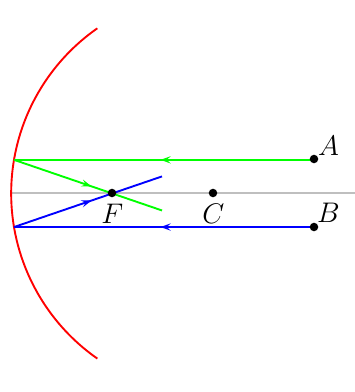
\includegraphics{fig12694_1.png}
}
\subfigure[Passage virtuel, miroir convexe]{%
    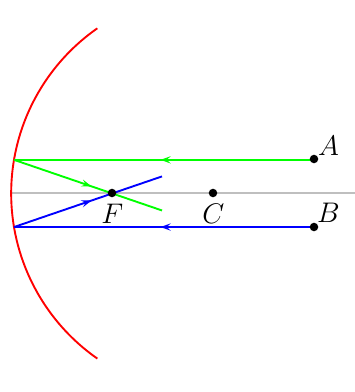
\includegraphics{fig12694_1.png}
}
\caption{Miroir sphérique : admirez comme tous les rayons parallèles à l'axe se réfléchissent en passant par le foyer !}  \label{FigPasageFoyer}
\end{figure}

\subsection{Construction de l'image d'un objet}
%----------------------------------------------

Muni des lois de la page \pageref{PgLoiMirSph}, nous sommes à même de construire l'image d'un objet $AB$. La figure \ref{FigMiroirSpherique} donne un exemple de la construction de l'image d'un point. Lorsqu'on a un segment $AB$ dont il faut calculer l'image, le plus simple est de choisir l'axe optique de telle façon à contenir le point $A$ et être perpendiculaire à $AB$. 

\begin{figure}
\centering
    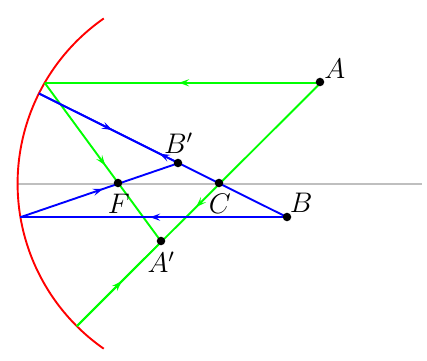
\includegraphics{fig29073_1.png}
\caption{Miroir sphérique : deux exemples de construction d'images de points. Un peu confus hein ? Essaie de refaire le dessin toi-même, et ça te paraîtra plus simple.}  \label{FigMiroirSpherique}
\end{figure}

Regardons pas à pas la construction de la figure \ref{FigConcUn}. Sur la figure \ref{FigConcUnPara}, nous avons tracé le rayon issu de $B$, et trouvé son intersection avec le miroir. En vertu d'une des lois (laquelle ?) de la page \ref{PgLoiMirSph}, ce rayon va se refléter en passant par le foyer (qui se trouve, rappelons-le, au milieu du segment d'axe optique joignant le centre du miroir et le miroir), comme montré sur la figure \ref{FigConcUnFoyer}. Pour terminer de fixer l'objet, on construit l'autre chemin facile : celui du rayon issu de $B$ qui tombe sur le miroir en passant par le centre. Celui-là est dessiné sur la figure \ref{FigConcUnCentre}.

\begin{figure}
\centering
\subfigure[D'abord, tracer le rayon issu de $A$ parallèlement à l'axe optique, et trouver le point $I$ où ce rayon tombe sur le miroir]{%
    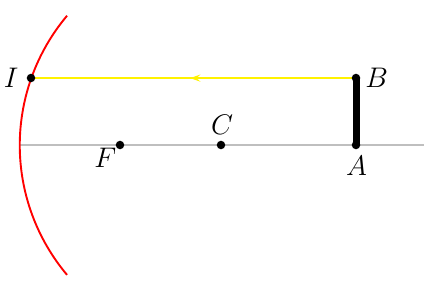
\includegraphics{fig7954_1.png}
\label{FigConcUnPara}
}
\subfigure[Ce rayon se reflète en passant par le foyer]{%
    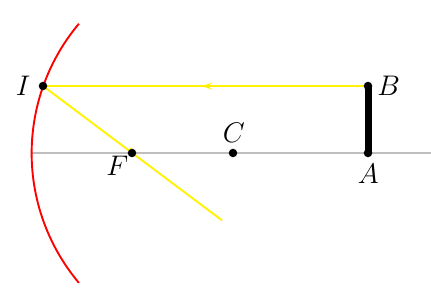
\includegraphics{fig7954_2.png}
\label{FigConcUnFoyer}
}
\subfigure[Le rayon issu de $B$ passant par le centre optique est reflété sur lui-même.]{%
    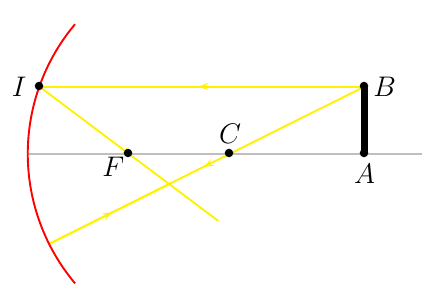
\includegraphics{fig7954_3.png}
\label{FigConcUnCentre}
}
\subfigure[L'intersection des deux rayons donne l'image de $B$, et permet de construire l'image de l'objet]{%
    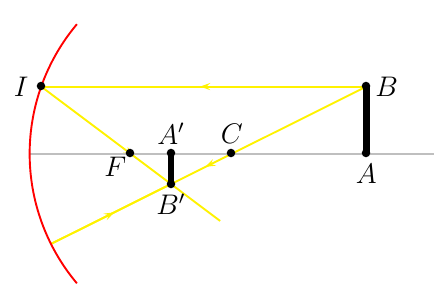
\includegraphics{fig7954_4.png}
\label{FigConcUnReponse}
}
\caption{Construction de l'image d'un objet}  \label{FigConcUn}
\end{figure}

Admirons maintenant sur la figure \ref{FigCasConcaves} différents cas que l'on peut trouver parmi les miroirs concaves. 

Il faut en particulier remarquer le passage virtuel sur la figure \ref{FigCasConcavesa} : le trajet que les rayons font en réalité est de se refléter sur le miroir et de diverger (contrairement aux deux autre cas).

\begin{figure}
\centering
\subfigure[Si l'objet se trouve au-delà du centre de courbure, l'image est renversée et plus petite que l'objet. De plus l'image est faire de rayons issus de l'objet lui-même, elle est donc réelle.]{
    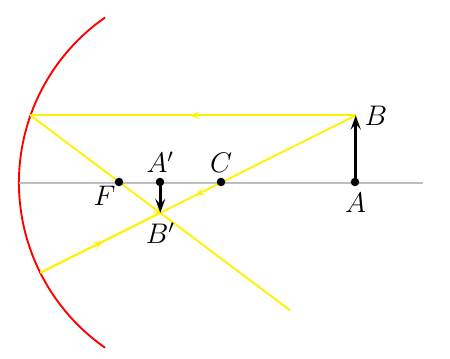
\includegraphics{fig28708_1.png}
\label{SubFigAudela}
}
\subfigure[Si l'objet se trouve entre le centre de courbure et le foyer, l'image est renversée, plus grande que l'objet et réelle.]{
    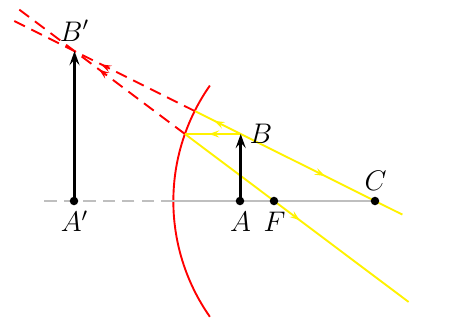
\includegraphics{fig28708_3.png}
}
\subfigure[Si l'objet se trouve entre le foyer et le miroir, l'image est droite, plus grande que l'objet et virtuelle. Les lignes en traits discontinus ne correspondent pas à un trajet que la lumière suit réellement : il n'y a pas de lumière à cet endroit.]{
    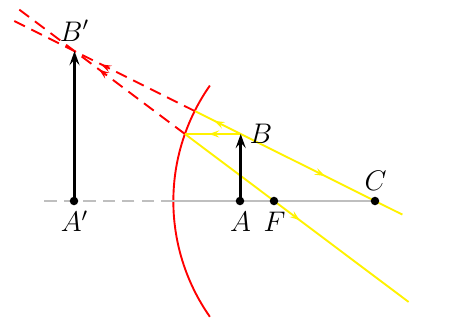
\includegraphics{fig28708_3.png}
\label{FigCasConcavesa}
}
\caption{Différents cas possibles avec un miroir concave.}  \label{FigCasConcaves}
\end{figure}

Le cas des miroirs convexes est exactement le même, sauf qu'on a plus souvent des passages virtuels. En suivant la méthode montrée à la figure \ref{FigConcUn}, nous obtenons la figure \ref{FigConvexeEx}.

\subsection{Quelque formules}
%----------------------------

En étudiant des triangles semblables sur la figure \ref{SubFigAudela} par exemple, nous pouvons établir les formules suivantes :
\begin{subequations}
\begin{equation}
  \frac{1}{ d }+\frac{1}{ d' }=\frac{1}{ f }\\
\end{equation}
\begin{equation}
   -\frac{ h' }{ h }=\frac{ d' }{ d }
\end{equation}
\end{subequations}
où $d'=\| SA' \|$ est la distance entre le miroir et l'image de l'objet, $d=\| SA \|$ est celle entre le miroir et l'objet, $h=\| AB \|$  et $h'=\| A'B' \|$ sont les tailles respectivement de l'objet et de son image ($f$ est la distance focale, c'est à dire la moitié du rayon du miroir sphérique). Nous prenons les conventions suivantes :
\begin{align*}
   f&=\text{ distance focale}\\
	&\quad >0\text{ pour un miroir concave}\\
	&\quad <0\text{ pour un miroir convexe}\\
  d&=\text{ distance de l'objet au miroir,}\\
  d'&=\text{ distance de l'image au mioir}\\
	&\quad >0\text{ pour une image réelle}\\
	&\quad <0\text{ pour une image virtuelle}\\
  h&=\text{ hauteur de l'objet}\\
  h'&=\text{ hauteur de l'image}\\
	&\quad >0\text{ pour une image droite}\\
	&\quad <0\text{ pour une image renversée}\\
\end{align*}
Le rapport $h'/h$ est souvent appelé l'\defe{agrandissement}{} du miroir.

\begin{figure}
\centering
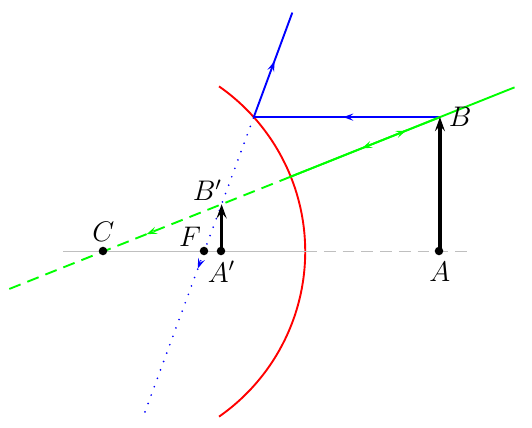
\includegraphics{fig27144_1.png}
\caption{L'image est droite, plus petite que l'objet et virtuelle.}  \label{FigConvexeEx}
\end{figure}

	% This is part of Un soupçon de physique, sans être agressif pour autant
% Copyright (C) 2006-2009
%   Laurent Claessens
% See the file fdl-1.3.txt for copying conditions.


%%%%%%%%%%%%%%%%%%%%%%%%%%
%
   \section{Lentilles minces}			\label{SecLentMinces}
%
%%%%%%%%%%%%%%%%%%%%%%%%

\subsection{Généralités et un peu de vocabulaire}
%------------------------------------------------

%http://fr.wikipedia.org/wiki/Homogène
En parlant de lentilles minces, nous n'allons parler que de \defe{lentilles sphériques}{}, c'est à dire des milieux transparents \href{http://fr.wikipedia.org/wiki/Homogène}{homogènes}\footnote{Dictionnaire.} limité par des surfaces sphériques. Commençons par un peu de vocabulaire :
\begin{description}
\item[Rayons de courbure] ce sont les rayons $R$ et $R'$ des surfaces sphériques qui délimitent la lentille,
\item[Centres de courbure] les centres $C$ et $C'$ des surfaces sphériques,
\item[Axe principal] la droite joignant les deux centres de courbure
\item[Lentilles à bords minces] celles de la figure \ref{FigLentilleBordMince},
\item[Lentilles à bords épais] celles de la figure \ref{FigLentilleBordEpais}.
\item[Lentilles convergentes]  Si on fait passer de la lumière solaire à travers une lentille à bords minces, on constate que la lumière se concentre en un point. On dit que la lentille est convergente et ce point s'appelle \defe{foyer}{} de la lentille.
\item[Lentilles divergentes] À travers une lentille à bords épais, il se forme un faisceau divergent. Une telle lentille est dite divergentes. Les rayons semblent issus d'un point appelé \defe{foyer}{} de la lentille.
\item[Centre optique] Lorsque les deux lentilles ont le même rayon, le centre optique est le centre de la lentille. Ce centre optique n'est pas spécialement le centre d'aucune des deux lentilles.
\end{description}

À propos, est-ce que tu sais pourquoi on dit qu'une droite est un cercle de rayon infini ? Parce que plus le rayon d'un cercle est grand, moins le cercle est courbé, plus il ressemble à une droite. La Terre par exemple fait \unit{6500}{\kilo\meter} de rayon, et effectivement elle semble assez plate. 

\begin{exercice}
À quel type de miroir te fait penser un croissant de Lune ? Et quand la Lune est pleine ?
\end{exercice}


\begin{figure}
\centering
\subfigure[biconvexe]{%
\begin{pspicture}(-2,-1.5)(3,1.5)
 %  \psframe[linecolor=cyan](-2,-1.5)(3,1.5)
   \psset{PointSymbol=none,PointName=none}
	\pstGeonode(-1,0){C}(0,1.5){S1}(0,-1.5){S2}(2,0){C'}
	\pstHomO[HomCoef=1.3]{C'}{C}[Cl]
	\pstHomO[HomCoef=1.3]{C}{C'}[Cpl]
	\psline[linecolor=lightgray](Cl)(Cpl)
	\pstArcOAB{C}{S2}{S1}
	\pstArcOAB{C'}{S1}{S2}
	\pstRotation[RotAngle=30]{C}{C'}[T1l]
	\pstRotation[RotAngle=20]{C'}{C}[T2l]
	\pstInterLC{C}{T1l}{C}{S1}{T1r}{T1}
	\pstInterLC{C'}{T2l}{C'}{S1}{T2r}{T2}
	\pstMarquePoint[PointSymbol=*]{C}{0.3;270}{$C$}
	\pstMarquePoint[PointSymbol=*]{C'}{0.3;270}{$C'$}
  \psline{->}(C)(T1)
   \pstMiddleAB{C}{T1}{inter}
   \pstMarquePoint{inter}{0.3;-45}{$R_{1}$}
  \psline{->}(C')(T2)
   \pstMiddleAB{C'}{T2}{inter}
   \pstMarquePoint{inter}{0.3;-45}{$R_{2}$}
\end{pspicture}
}
\subfigure[plan-convexe]{%
\begin{pspicture}(-2,-1.5)(3,1.5)
 %  \psframe[linecolor=cyan](-2,-1.5)(3,1.5)
   \psset{PointSymbol=none,PointName=none}
	\pstGeonode(-1,0){C}(0,1.5){S1}(0,-1.5){S2}(2,0){C'}
	\pstHomO[HomCoef=1.3]{C'}{C}[Cl]
	\pstHomO[HomCoef=1.3]{C}{C'}[Cpl]
	\psline[linecolor=lightgray](Cl)(Cpl)
	\pstArcOAB{C}{S2}{S1}
	\psline(S1)(S2)
	\pstRotation[RotAngle=30]{C}{C'}[T1l]
	\pstRotation[RotAngle=20]{C'}{C}[T2l]
	\pstInterLC{C}{T1l}{C}{S1}{T1r}{T1}
	\pstInterLC{C'}{T2l}{C'}{S1}{T2r}{T2}
	\psline{->}(C)(T1)
	\pstInterLL{C'}{T2}{S1}{S2}{I1}
	\pstTranslation{C}{I1}{C'}[I1l]
	\psline{->}(I1l)(I1)
	\pstMarquePoint[PointSymbol=*]{C}{0.3;270}{$C$}

   \pstMiddleAB{C}{T1}{inter}
   \pstMarquePoint{inter}{0.3;120}{$R_{1}$}
   \pstMiddleAB{I1l}{I1}{inter}
   \pstMarquePoint{inter}{0.5;-45}{$R_{2}=\infty$}

\end{pspicture}
}
\subfigure[concave-convexe]{%
\begin{pspicture}(-3,-1.5)(1.5,1.5)
%   \psframe[linecolor=cyan](-3,-1.5)(1.5,1.5)
   \psset{PointSymbol=none,PointName=none}
	\pstGeonode(-0.6,0){C}(0,1.5){S1}(0,-1.5){S2}(-2,0){C'}
	\pstHomO[HomCoef=2.5]{C'}{C}[Cl]
	\pstHomO[HomCoef=1.3]{C}{C'}[Cpl]
	\psline[linecolor=lightgray](Cl)(Cpl)
	\pstArcOAB{C}{S2}{S1}
	\pstArcOAB{C'}{S2}{S1}
	\pstRotation[RotAngle=-30]{C}{C'}[T1l]
	\pstRotation[RotAngle=20]{C'}{C}[T2l]
	\pstInterLC{C}{T1l}{C}{S2}{T1}{T1r}
	\pstInterLC{C'}{T2l}{C'}{S1}{T2r}{T2}
	\pstMarquePoint[PointSymbol=*]{C}{0.3;270}{$C$}
	\pstMarquePoint[PointSymbol=*]{C'}{0.3;270}{$C'$}
  \psline{->}(C)(T1)
   \pstMiddleAB{C}{T1}{inter}
   \pstMarquePoint{inter}{0.3;-130}{$R_{1}$}
  \psline{->}(C')(T2)
   \pstMiddleAB{C'}{T2}{inter}
   \pstMarquePoint{inter}{0.3;90}{$R_{2}$}
\end{pspicture}
}


\caption{Des lentilles à bords minces}  \label{FigLentilleBordMince}
\end{figure}

\begin{figure}
\centering

\subfigure[biconcave]{%
\begin{pspicture}(-1.8,-1.5)(3.5,1.5)
 %  \psframe[linecolor=cyan](-1.8,-1.5)(3.5,1.5)
   \psset{PointSymbol=none,PointName=none}
	\pstGeonode(-1,0){C}(3,0){C'}(0,1.5){S1}
	\pstTransHom{C}{C'}{S1}{0.7}{T1}
	\pstOrtSym{C}{C'}{S1}[S2]
	\pstOrtSym{C}{C'}{T1}[T2]
	\psline(S1)(T1)\psline(S2)(T2)

	\pstHomO[HomCoef=1.2]{C'}{C}[Cl]
	\pstHomO[HomCoef=1.2]{C}{C'}[Cpl]
	\psline[linecolor=lightgray](Cl)(Cpl)

	\pstArcOAB{C}{S2}{S1}
	\pstArcOAB{C'}{T1}{T2}
	
	\pstRotation[RotAngle=30]{C}{C'}[P1l]
	\pstInterLC{C}{P1l}{C}{S1}{T1r}{P1}

	\pstInterLC{C'}{S2}{C'}{T1}{PT'}{PT}

	\pstMarquePoint[PointSymbol=*]{C}{0.3;270}{$C$}
	\pstMarquePoint[PointSymbol=*]{C'}{0.3;90}{$C'$}


   \psline{->}(C)(P1)	
   \pstMiddleAB{C}{P1}{inter}
   \pstMarquePoint{inter}{0.3;130}{$R_{1}$}
	
   \psline{->}(C')(PT)	
   \pstMiddleAB{C'}{PT}{inter}
   \pstMarquePoint{inter}{0.3;-45}{$R_{2}$}

\end{pspicture}
}

\subfigure[plan-concave]{%
\begin{pspicture}(-1.8,-1.5)(3.5,1.5)
 %  \psframe[linecolor=cyan](-1.8,-1.5)(3.5,1.5)
   \psset{PointSymbol=none,PointName=none}
	\pstGeonode(-1,0){C}(2,0){C'}(0,1.5){S1}
	\pstTransHom{C}{C'}{S1}{0.4}{T1}
	\pstOrtSym{C}{C'}{S1}[S2]
	\pstOrtSym{C}{C'}{T1}[T2]
	\psline(S1)(T1)\psline(S2)(T2)

	\pstHomO[HomCoef=1.2]{C'}{C}[Cl]
	\pstHomO[HomCoef=1.2]{C}{C'}[Cpl]
	\psline[linecolor=lightgray](Cl)(Cpl)

	\pstArcOAB{C}{S2}{S1}
	\psline(T1)(T2)
	
	\pstRotation[RotAngle=30]{C}{C'}[P1l]
	\pstInterLC{C}{P1l}{C}{S1}{T1r}{P1}
	\pstMarquePoint[PointSymbol=*]{C}{0.3;270}{$C$}

	\pstHomO[HomCoef=0.7]{T1}{T2}[T12]
	\pstTransHom{S1}{T1}{T12}{1.5}{inf}
	

   \psline{->}(C)(P1)
   \pstMiddleAB{C}{P1}{inter}
   \pstMarquePoint{inter}{0.3;130}{$R_{1}$}
	
   \psline{->}(inf)(T12)
   \pstMiddleAB{inf}{T12}{inter}
   \pstMarquePoint{inter}{0.3;270}{$R_{2}=\infty$}

\end{pspicture}
}
\subfigure[convexe-concave]{%
\begin{pspicture}(-4,-1.5)(2,1.5)
%   \psframe[linecolor=cyan](-4,-1.5)(2,1.5)
   \psset{PointSymbol=none,PointName=none}
	\pstGeonode(-0.7,0){C}(-3,0){C'}(0,1.5){S1}
	\pstTransHom{C}{C'}{S1}{-0.5}{T1}
	\pstOrtSym{C}{C'}{S1}[S2]
	\pstOrtSym{C}{C'}{T1}[T2]
	\psline(S1)(T1)\psline(S2)(T2)

	\pstHomO[HomCoef=2]{C'}{C}[Cl]
	\pstHomO[HomCoef=1.2]{C}{C'}[Cpl]
	\psline[linecolor=lightgray](Cl)(Cpl)

	\pstArcOAB{C}{S2}{S1}
	\pstArcOAB{C'}{T2}{T1}
	
	\pstRotation[RotAngle=30]{C}{C'}[P1l]
	\pstInterLC{C}{P1l}{C}{S1}{P1}{T1r}

	\pstRotation[RotAngle=-15]{C'}{C}[Q1l]
	\pstInterLC{C'}{Q1l}{C'}{T1}{Qr}{Q}

	\pstMarquePoint[PointSymbol=*]{C}{0.3;90}{$C$}
	\pstMarquePoint[PointSymbol=*]{C'}{0.3;90}{$C'$}

	%\pstMarquePoint[PointSymbol=*]{S1}{0.3;90}{$S1$}
	%\pstMarquePoint[PointSymbol=*]{T1}{0.3;90}{$T1$}
	%\pstMarquePoint[PointSymbol=*]{S2}{0.3;90}{$S2$}
	%\pstMarquePoint[PointSymbol=*]{T2}{0.3;90}{$T2$}

   \psline{->}(C)(P1)	
   \pstMiddleAB{C}{P1}{inter}
   \pstMarquePoint{inter}{0.3;130}{$R_{1}$}
	
   \psline{->}(C')(Q)
   \pstMiddleAB{C'}{Q}{inter}
   \pstMarquePoint{inter}{0.3;-90}{$R_{2}$}

\end{pspicture}
}
\caption{Des lentilles à bords épais}  \label{FigLentilleBordEpais}
\end{figure}

\subsection{Propriétés des lentilles minces}
%-------------------------------------------

Un rayon lumineux qui traverse une lentille subit deux réfractions\footnote{Une en passant de l'air au verre au moment de rentrer et une du verre à l'air au moment de sortir.}, ce qui rend l'étude du trajet plus compliquée. Heureusement, si la lentille est suffisamment mince, nous pouvons quand même suivre les lois simples suivantes :

\setcounter{numloiphyz}{0}		% Note qu'il faudra souvent le remettre à zéro ce compteur. Genre à tous les coups.
\begin{loiphyz}
Un rayon lumineux passant par le centre optique d'une lentille mince ne subit aucune déviation.
\end{loiphyz}

\begin{loiphyz}
Un rayon lumineux parallèle à l'axe principal se réfracte en passant réellement ou virtuellement par le foyer.
\end{loiphyz}

\begin{loiphyz}
Un rayon passant réellement ou virtuellement par le foyer se réfracte parallèlement à l'axe principal.
\end{loiphyz}

Ces lois ne sont que des approximations de la réalité, mais il se fait que ces approximations restent bonnes même pour des rayons fortement inclinés (pourvu que la lentille soit suffisamment mince).

\label{PgRemarqueFoyer}Une lentille possède toujours deux foyers : un de chaque côté. Donc il faut un peu préciser les deux dernières lois pour savoir de quel foyer on parle.
\begin{description}
\item[Lentilles convergentes] Un rayon arrivant parallèlement à l'axe principal se reflète en passant par le foyer se trouvant \emph{de l'autre côté} de la lentille.
\item[Lentille divergente] Un rayon arrivant parallèlement à l'axe principale se reflète en passant (virtuellement) par le foyer situé \emph{du même côté} de la lentille.
\end{description}
Des exemples de passages à travers une lentille convergente sont donnés à la figure \ref{FigTroisPassagesConvergent}, et des passages à travers une divergente sont donnés à la figure \ref{FigTroisPassagesDivergents}

\begin{figure}
\centering
\subfigure[Un rayon arrive parallèlement à l'axe optique]{%
\begin{pspicture}(-2.5,-1.4)(2,1.5)
   %\psframe[linecolor=cyan](-2.5,-1.4)(2,1.5)
   \psset{PointSymbol=none,PointName=none}
	\pstGeonode(0,0){O}(1,0){F'}(-2,0.6){A}
	\pstSymO{O}{F'}[F]
	\pstTranslation{O}{F'}{A}[Al]
	\pstRotation[RotAngle=90]{O}{F'}[P]

	\pstSymO{O}{P}[P']
	\pstInterLL{Al}{A}{P}{O}{Q}
	\pstHomO[HomCoef=1.5]{Q}{F'}[Ql]

	\pstRayon[linecolor=red]{A}{Q}\pstRayon[linecolor=red]{Q}{Ql}
	\pstLineAB[nodesepA=-0.5,nodesepB=-0.5,linecolor=lightgray]{F}{F'}
	\psline{<->}(P)(P')
	\pstMarquePoint[PointSymbol=*]{F}{0.3;-90}{$F$}
	\pstMarquePoint[PointSymbol=*]{F'}{0.3;45}{$F'$}
	\pstMarquePoint[PointSymbol=*]{O'}{0.3;135}{$O$}
\end{pspicture} \label{FigTroisPassConva}
}
\subfigure[Un rayon arrive en passant par le foyer]{%
\begin{pspicture}(-2.5,-1.4)(2.3,1.5)
   %\psframe[linecolor=cyan](-2.5,-1.4)(2.3,1.5)
   \psset{PointSymbol=none,PointName=none}
	\pstGeonode(0,0){O}(1,0){F'}(-2.5,-0.8){A}
	\pstSymO{O}{F'}[F]
	\pstRotation[RotAngle=90]{O}{F'}[P]

	\pstSymO{O}{P}[P']
	\pstInterLL{F}{A}{P}{O}{Q}
	\pstTranslation{F}{F'}{Q}[Ql]

	\pstRayon[linecolor=red]{A}{Q}\pstRayon[linecolor=red]{Q}{Ql}
	\pstLineAB[nodesepA=-0.5,nodesepB=-0.5,linecolor=lightgray]{F}{F'}
	\psline{<->}(P)(P')
	\pstMarquePoint[PointSymbol=*]{F}{0.3;-90}{$F$}
	\pstMarquePoint[PointSymbol=*]{F'}{0.3;45}{$F'$}
	\pstMarquePoint[PointSymbol=*]{O'}{0.3;45}{$O$}
\end{pspicture}\label{FigTroisPassConvb}
}
\subfigure[Un rayon arrive en passant par le centre optique]{%
\begin{pspicture}(-2,-1.4)(2.3,1.5)
   %\psframe[linecolor=cyan](-2,-1.4)(2.3,1.5)
   \psset{PointSymbol=none,PointName=none}
	\pstGeonode(0,0){O}(1,0){F'}(-1.5,-1){A}
	\pstSymO{O}{F'}[F]
	\pstRotation[RotAngle=90]{O}{F'}[P]

	\pstSymO{O}{P}[P']
	\pstHomO[HomCoef=2.3]{A}{O}[Al]

	\pstRayon[linecolor=red]{A}{O}\pstRayon[linecolor=red]{O}{Al}
	\pstLineAB[nodesepA=-0.5,nodesepB=-0.5,linecolor=lightgray]{F}{F'}
	\psline{<->}(P)(P')
	\pstMarquePoint[PointSymbol=*]{F}{0.3;-90}{$F$}
	\pstMarquePoint[PointSymbol=*]{F'}{0.3;45}{$F'$}
	\pstMarquePoint[PointSymbol=*]{O'}{0.3;135}{$O$}
\end{pspicture}\label{FigTroisPassConvc}
}
\caption{Trois passages possibles à travers une lentille convergente.}  \label{FigTroisPassagesConvergent}
\end{figure}


\begin{figure}
\centering
\subfigure[Un rayon arrive parallèlement à l'axe optique]{%
\begin{pspicture}(-2.5,-1.4)(2,1.5)
   %\psframe[linecolor=cyan](-2.5,-1.4)(2,1.5)
   \psset{PointSymbol=none,PointName=none}
	\pstGeonode(0,0){O}(1,0){F'}(-2,0.6){A}
	\pstSymO{O}{F'}[F]
	\pstTranslation{O}{F'}{A}[Al]
	\pstRotation[RotAngle=90]{O}{F'}[P]

	\pstSymO{O}{P}[P']
	\pstInterLL{Al}{A}{P}{O}{Q}
	\pstHomO[HomCoef=2]{F}{Q}[Ql]

	\pstRayon[linecolor=red]{A}{Q}
	\pstRayon[linecolor=red]{Q}{Ql}
	\pstRayon[linecolor=red,linestyle=dashed]{F}{Q}

	\pstLineAB[nodesepA=-0.5,nodesepB=-0.5,linecolor=lightgray]{F}{F'}
	\psline{>-<}(P)(P')
	\pstMarquePoint[PointSymbol=*]{F}{0.3;-90}{$F$}
	\pstMarquePoint[PointSymbol=*]{F'}{0.3;45}{$F'$}
	\pstMarquePoint[PointSymbol=*]{O'}{0.3;45}{$O$}
\end{pspicture}
}
\subfigure[Un rayon arrive en passant par le foyer]{%
\begin{pspicture}(-2.5,-1.4)(2.3,1.5)
   %\psframe[linecolor=cyan](-2.5,-1.4)(2.3,1.5)
   \psset{PointSymbol=none,PointName=none}
	\pstGeonode(0,0){O}(1,0){F'}(-1,-1.3){A}
	\pstSymO{O}{F'}[F]
	\pstRotation[RotAngle=90]{O}{F'}[P]
	\pstSymO{O}{P}[P']

	\pstInterLL{F'}{A}{P}{O}{Q}
	\pstTranslation{F}{F'}{Q}[Ql]

	\pstRayon[linecolor=red]{A}{Q}
	\pstRayon[linecolor=red]{Q}{Ql}
	\pstRayon[linecolor=red,linestyle=dashed]{Q}{F'}

	\pstLineAB[nodesepA=-0.5,nodesepB=-0.5,linecolor=lightgray]{F}{F'}
	\psline{>-<}(P)(P')
	\pstMarquePoint[PointSymbol=*]{F}{0.3;-90}{$F$}
	\pstMarquePoint[PointSymbol=*]{F'}{0.3;45}{$F'$}
	\pstMarquePoint[PointSymbol=*]{O'}{0.3;45}{$O$}
\end{pspicture}
}
\subfigure[Un rayon arrive en passant par le centre optique]{%
\begin{pspicture}(-2,-1.4)(2.3,1.5)
   %\psframe[linecolor=cyan](-2,-1.4)(2.3,1.5)
   \psset{PointSymbol=none,PointName=none}
	\pstGeonode(0,0){O}(1,0){F'}(-1.5,-1){A}
	\pstSymO{O}{F'}[F]
	\pstRotation[RotAngle=90]{O}{F'}[P]

	\pstSymO{O}{P}[P']
	\pstHomO[HomCoef=2.3]{A}{O}[Al]

	\pstRayon[linecolor=red]{A}{O}\pstRayon[linecolor=red]{O}{Al}
	\pstLineAB[nodesepA=-0.5,nodesepB=-0.5,linecolor=lightgray]{F}{F'}
	\psline{>-<}(P)(P')
	\pstMarquePoint[PointSymbol=*]{F}{0.3;-90}{$F$}
	\pstMarquePoint[PointSymbol=*]{F'}{0.3;45}{$F'$}
	\pstMarquePoint[PointSymbol=*]{O'}{0.3;135}{$O$}
\end{pspicture}
}
\caption{Trois passages possibles à travers une lentille divergente.}  \label{FigTroisPassagesDivergents}
\end{figure}

\subsection{Image d'un objet}
%----------------------------

Lorsque nous avons un objet dont il faut trouver l'image, c'est très simple : nous devons trouver le trajet de deux rayons qui s'en échappent et l'image sera à l'intersection (réelle ou virtuelle d'après les cas).

\begin{figure}
\centering
\subfigure[Si l'objet se trouve à une grande distance de la lentille, l'image est réelle, renversée et plus petite que l'objet. Remarque que les rayon rouges suivent le trajet de la figure \ref{FigTroisPassConvb}, tandis que les bleus correspondent à \ref{FigTroisPassConva}. Je te laisse voir à quoi correspond le rayon vert.]{%
\begin{pspicture}(-6,-2)(4,2)
  % \psframe[linecolor=cyan](-4,-2)(4,2)
   \psset{PointSymbol=none,PointName=none}
	\pstGeonode(0,0){O}(-2,0){F}(-6,1.5){A}
	\pstGeonode(-6,0){L1}(4,0){L2}
% Calculs	
	\pstLentille{O}{F}{A}{Q}{iA}{B}{iB}
	\pstRotation[RotAngle=90]{O}{F}[P]
	\pstSymO{O}{P}[P']
	\pstSymO{O}{F}[F']
	\pstProjectionOrth{O}{P}{A}{Q'}

% Tracé
	\psline{<->}(P)(P')
	\pstRayon[linecolor=red,ArrowInsidePos=0.25]{A}{Q}
 	\pstRayon[linecolor=red]{Q}{iA} 
	\pstRayon[linecolor=green]{A}{O}\pstRayon[linecolor=green]{O}{iA}
	\pstRayon[linecolor=blue]{A}{Q'}
	\pstRayon[linecolor=blue,ArrowInsidePos=0.25]{Q'}{iA}
	\psline[linecolor=lightgray](L1)(L2)

\psline[linewidth=0.05]{->}(iB)(iA)
\psline[linewidth=0.05]{->}(B)(A)

	\pstMarquePoint[PointSymbol=*]{A}{0.3;90}{$A$}
	\pstMarquePoint[PointSymbol=*]{F}{0.3;90}{$F$}
	\pstMarquePoint[PointSymbol=*]{F'}{0.3;90}{$F'$}
	\pstMarquePoint[PointSymbol=*]{O}{0.3;45}{$O$}
	\pstMarquePoint[PointSymbol=*]{iA}{0.3;-90}{$A'$}

\end{pspicture}\label{FigImageConva}
}
\subfigure[Si l'objet se trouve à une distance égale au double de la distance focale, l'image est réelle, renversée et de même grandeur que l'objet.]{%
\begin{pspicture}(-4,-2)(4,2)
   %\psframe[linecolor=cyan](-4,-2)(4,2)
   \psset{PointSymbol=none,PointName=none}
	\pstGeonode(0,0){O}(-2,0){F}(-4,1.5){A}
	\pstGeonode(-4,0){L1}(4,0){L2}
% Calculs	
	\pstLentille{O}{F}{A}{Q}{iA}{B}{iB}
	\pstRotation[RotAngle=90]{O}{F}[P]
	\pstSymO{O}{P}[P']
	\pstSymO{O}{F}[F']
	\pstProjectionOrth{O}{P}{A}{Q'}

% Tracé
	\psline{<->}(P)(P')
	%\pstRayon[linecolor=red,ArrowInsidePos=0.25]{A}{Q}
 	%\pstRayon[linecolor=red]{Q}{iA} 
	\pstRayon[linecolor=green]{A}{O}\pstRayon[linecolor=green]{O}{iA}
	\pstRayon[linecolor=blue]{A}{Q'}
	\pstRayon[linecolor=blue,ArrowInsidePos=0.75]{Q'}{iA}
	\psline[linecolor=lightgray](L1)(L2)

\psline[linewidth=0.05]{->}(iB)(iA)
\psline[linewidth=0.05]{->}(B)(A)

	\pstMarquePoint[PointSymbol=*]{A}{0.3;90}{$A$}
	\pstMarquePoint[PointSymbol=*]{F}{0.3;90}{$F$}
	\pstMarquePoint[PointSymbol=*]{F'}{0.3;90}{$F'$}
	\pstMarquePoint[PointSymbol=*]{O}{0.3;45}{$O$}
	\pstMarquePoint[PointSymbol=*]{iA}{0.3;-90}{$A'$}

\end{pspicture} \label{FigImageConvb}
}
\subfigure[Si l'objet se trouve à une distance comprise entre $f$ et $2f$ ($f=$ distance focale), l'image est réelle, renversée et plus grande que l'objet.]{%
\begin{pspicture}(-4,-3.5)(6,2)
   %\psframe[linecolor=cyan](-4,-3.5)(6,2)
   \psset{PointSymbol=none,PointName=none}
	\pstGeonode(0,0){O}(-2,0){F}(-3,1.5){A}
	\pstGeonode(-4,0){L1}(6,0){L2}
% Calculs	
	\pstLentille{O}{F}{A}{Q}{iA}{B}{iB}
	\pstRotation[RotAngle=90]{O}{F}[P]
	\pstSymO{O}{P}[P']
	\pstSymO{O}{F}[F']
	\pstProjectionOrth{O}{P}{A}{Q'}

% Tracé
	\psline{<->}(P)(P')
	%\pstRayon[linecolor=red,ArrowInsidePos=0.25]{A}{Q}
 	%\pstRayon[linecolor=red]{Q}{iA} 
	\pstRayon[linecolor=green]{A}{O}\pstRayon[linecolor=green]{O}{iA}
	\pstRayon[linecolor=blue]{A}{Q'}
	\pstRayon[linecolor=blue,ArrowInsidePos=0.75]{Q'}{iA}
	\psline[linecolor=lightgray](L1)(L2)

\psline[linewidth=0.05]{->}(iB)(iA)
\psline[linewidth=0.05]{->}(B)(A)

	\pstMarquePoint[PointSymbol=*]{A}{0.3;90}{$A$}
	\pstMarquePoint[PointSymbol=*]{F}{0.3;90}{$F$}
	\pstMarquePoint[PointSymbol=*]{F'}{0.3;90}{$F'$}
	\pstMarquePoint[PointSymbol=*]{O}{0.3;45}{$O$}
	\pstMarquePoint[PointSymbol=*]{iA}{0.3;-90}{$A'$}

\end{pspicture} \label{FigImageConvc}
}
\subfigure[Si l'objet se trouve entre le foyer et le centre optique, l'image est virtuelle, droite et plus grande que l'objet.]{%
\begin{pspicture}(-4,-2)(3.5,3.5)
   %\psframe[linecolor=cyan](-4,-2)(3.5,3.5)
   \psset{PointSymbol=none,PointName=none}
	\pstGeonode(0,0){O}(-2,0){F}(-1.1,1.5){A}
	\pstGeonode(-4,0){L1}(3.5,0){L2}
% Calculs	
	\pstLentille{O}{F}{A}{Q}{iA}{B}{iB}
	\pstRotation[RotAngle=90]{O}{F}[P]
	\pstSymO{O}{P}[P']
	\pstSymO{O}{F}[F']
	\pstProjectionOrth{O}{P}{A}{Q'}
	\pstHomO[HomCoef=1.5]{Q'}{F'}[QF]
	\pstHomO[HomCoef=1.5]{A}{O}[AO]

% Tracé
	\psline{<->}(P)(P')
	%\pstRayon[linecolor=red,ArrowInsidePos=0.25]{A}{Q}
 	%\pstRayon[linecolor=red]{Q}{iA} 
	\pstRayon[linecolor=green]{A}{AO}\pstRayon[linecolor=green,linestyle=dashed]{A}{iA}
	\pstRayon[linecolor=blue]{Q'}{QF}
	\pstRayon[linecolor=blue]{A}{Q'}
	\pstRayon[linecolor=blue,linestyle=dashed]{Q'}{iA}
	\psline[linecolor=lightgray](L1)(L2)

\psline[linewidth=0.05,linestyle=dashed]{->}(iB)(iA)
\psline[linewidth=0.05]{->}(B)(A)

	\pstMarquePoint[PointSymbol=*]{A}{0.3;90}{$A$}
	\pstMarquePoint[PointSymbol=*]{F}{0.3;-90}{$F$}
	\pstMarquePoint[PointSymbol=*]{F'}{0.3;45}{$F'$}
	\pstMarquePoint[PointSymbol=*]{O}{0.3;45}{$O$}
	\pstMarquePoint[PointSymbol=*]{iA}{0.3;180}{$A'$}

\end{pspicture} \label{FigImageConvd}
}
\caption{Construction d'images d'objets par une lentille convergentes.}  \label{FigImageConv}
\end{figure}

\begin{figure}
\centering
\begin{pspicture}(-4,-2)(4,2)
   %\psframe[linecolor=cyan](-4,-2)(4,2)
   \psset{PointSymbol=none,PointName=none}
	 %\psframe[linecolor=cyan](-4,-2)(3.5,3.5)
   \psset{PointSymbol=none,PointName=none}
	\pstGeonode(0,0){O}(-2,0){F}(-3,1.7){A}
	\pstGeonode(-4,0){L1}(3.5,0){L2}
% Calculs	
	\pstSymO{O}{F}[F']
	\pstLentille{O}{F'}{A}{Q}{iA}{B}{iB}
	\pstRotation[RotAngle=90]{O}{F}[P]
	\pstSymO{O}{P}[P']
	\pstProjectionOrth{O}{P}{A}{Q'}
	\pstHomO[HomCoef=1.5]{Q'}{F'}[QF']
	\pstHomO[HomCoef=1.5]{Q'}{F}[QF]
	\pstHomO[HomCoef=1.5]{A}{O}[AO]
% Tracé
	\psline{<->}(P)(P')
	%\pstRayon[linecolor=red,ArrowInsidePos=0.25]{A}{Q}
 	%\pstRayon[linecolor=red]{Q}{iA} 
	\pstRayon[linecolor=green]{A}{AO}\pstRayon[linecolor=green,linestyle=dashed]{A}{iA}
	\pstRayon[linecolor=blue]{Q'}{QF'}
	\pstRayon[linecolor=blue]{A}{Q'}
	\pstRayon[linecolor=blue,linestyle=dashed]{Q'}{QF}
	\psline[linecolor=lightgray](L1)(L2)

\psline[linewidth=0.05,linestyle=dashed]{->}(iB)(iA)
\psline[linewidth=0.05]{->}(B)(A)

	\pstMarquePoint[PointSymbol=*]{A}{0.3;90}{$A$}
	\pstMarquePoint[PointSymbol=*]{F}{0.3;-90}{$F$}
	\pstMarquePoint[PointSymbol=*]{F'}{0.3;45}{$F'$}
	\pstMarquePoint[PointSymbol=*]{O}{0.3;45}{$O$}
	\pstMarquePoint[PointSymbol=*]{iA}{0.3;90}{$A'$}

\end{pspicture}

\caption{Un exemple de lentille divergente. Les lentille divergente ne fournissent que des images virtuelles, droites et plus petites que l'objet.}  \label{FigImageDivergent}
\end{figure}

\begin{exercice}
Complète les figures \ref{FigImageConvb}-\ref{FigImageConvd} en dessinant les rayons qui partent de $A$ en passant par le foyer, comme le rouge de la figure \ref{FigImageConva}.
\end{exercice}

\begin{exercice}
Il est dit dans la légende de la figure \ref{FigImageConvb} que l'image était de la même taille que l'objet. Peux-tu le prouver en utilisant ce que tu sais de la géométrie dans le plan ?
\end{exercice}

\begin{exercice}
Prouve, en t'inspirant des figures \ref{FigImageConv} que lorsque l'objet est placé \emph{sur} le foyer, les rayons réfléchis par la lentille sont parallèles. Dans ce cas, on dit que l'image est rejetée à l'infini.
\end{exercice}

\begin{remark}
Dans le cas où l'objet est placé sur le foyer, on dit que l'image est rejetée à l'infini en vertu de l'adage selon lequel \og deux droites parallèles se rejoignent à l'infini\fg{}. Sache que la géométrie euclidienne ne possède pas d'infini. En géométrie euclidienne, deux droites parallèles ne se rencontrent jamais. Ce n'est qu'au cours du XIX\ieme{} siècle que l'on inventa des points à l'infini dans le cadre de la \emph{géométrie projective}. Cette géométrie fut entre autres inventée pour les besoins des peintres et des architectes qui voulaient dessiner du relief. La géométrie projective et la façon dont deux droites parallèles se rejoignent à l'infini fait partie des choses que tu ne sauras que si tu décides de faire de la mathématique plus avancée.

Jusqu'à la figure \ref{FigImageConvd} (non comprise), l'image s'est toujours éloignée. Elle est arrivée à l'infini quand l'objet était sur le foyer. Et à la figure \ref{FigImageConvd}, elle revient \emph{de l'autre côté}. Un peu comme si l'infini à droite est accroché à l'infini à gauche. Cela est une des grande nouvelles en géométries projective : il n'y a qu'un seul infini pour chaque direction, et non un dans chaque sens.
\end{remark}

\paragraph{Image floue ?} Prends n'importe quelle figure \ref{FigImageConv} sauf la \ref{FigImageConvd} et demande-toi ce que tu vois si tu places ton \oe uil au point $F$ et que tu regardes dans la direction du rayon bleu. Ce que tu vois, c'est le point $A$. En effet, la lumière que ton \oe uil reçoit provient de $A$. Mais si tu regardes de la même manière le rayon vert au point $O$, tu verras aussi le point $A$. C'est à dire que l'image du point $A$ s'étale au moins sur tout le segment $OF$. Pas étonnant que ce soit flou !

Au point $A'$, tous les rayons issus de $A$ se coupent. Donc autour de $A'$, les rayons issus de $A$ sont fort \og regroupés\fg, ils ne s'étalent pas beaucoup. C'est pour cette raison que l'image de $A$ est nette au point $A'$. 

\begin{exercice}
Qu'est-ce que tu verrais si tu mettais ton \oe uil au point $A'$ de la figure \ref{FigImageConvd} ?
\end{exercice}

\subsection{Formules pour les lentilles minces}
%---------------------------------------------

Il est possible d'établir les deux formules suivantes :
\begin{equation}
  \frac{1}{ d }+\frac{1}{ d' }=\frac{1}{ f }\quad\text{et}\quad -\frac{ h' }{ h }=\frac{ d' }{ d }
\end{equation}
où $d$ est la distance entre le centre optique et l'objet, $d'$ est celle entre le centre optique et l'image, $f$ est la distance focale, $h$ est la taille de l'objet et $h'$ est celle de l'image. Fais un dessin et indique dessus ces différentes grandeurs. Les conventions suivantes ont cours :
\begin{align*}
   f&=\text{ distance focale}\\
	&\quad >0\text{ pour une lentille convergentes}\\
	&\quad <0\text{ pour une lentille divergente}\\
  d'&=\text{ distance de l'image centre optique}\\
	&\quad >0\text{ pour une image réelle}\\
	&\quad <0\text{ pour une image virtuelle}\\
  h'&=\text{ hauteur de l'image}\\
	&\quad >0\text{ pour une image droite}\\
	&\quad <0\text{ pour une image renversée}\\
\end{align*}
Ces conventions sont en accord avec ce que nous disions à la page \ref{PgRemarqueFoyer} à propos du fait que pour une lentille convergente, il fallait utiliser le foyer de l'autre côté pour les lentilles convergentes et le foyer du même côté pour les divergentes. À ce propos, regarde la figure \ref{FigLentilleObjDroite}.

%http://fr.wikipedia.org/wiki/Dioptrie
%http://fr.wikipedia.org/wiki/Vergence
Nous définissons aussi la \defe{\href{http://fr.wikipedia.org/wiki/Vergence}{vergence}}{} d'une lentille par
\[ 
  C=\frac{1}{ f }
\]
dont les unités sont $\reciprocal\meter$. Dans le cas des lentilles, l'unité \reciprocal\meter{} est appelée \href{http://fr.wikipedia.org/wiki/Dioptrie}{dioptrie}; on parle d'une lentille de $4$ dioptrie pour dire que sa vergence vaut \unit{4}{\reciprocal\meter}. Les conventions que nous avons prises font que $C>0$ pour les lentilles convergentes et $C<0$ pour les lentilles divergentes.

\begin{figure}
\centering
\subfigure[Un cas classique avec la formation de l'image d'un objet à travers une lentille convergente.]{%
\begin{pspicture}(-4,-3)(4,2)
  % \psframe[linecolor=cyan](-6,-2)(4,2)
   \psset{PointSymbol=none,PointName=none}
	\pstGeonode(0,0){O}(-2,0){F}(-6,1.5){A}
	\pstGeonode(-6,0){L1}(4,0){L2}
% Calculs	
	\pstLentille{O}{F}{A}{Q}{iA}{B}{iB}
	\pstRotation[RotAngle=90]{O}{F}[P]
	\pstSymO{O}{P}[P']
	\pstSymO{O}{F}[F']
	\pstProjectionOrth{O}{P}{A}{Q'}

% Tracé
	\psline{<->}(P)(P')
	\pstRayon[linecolor=red,ArrowInsidePos=0.25]{A}{Q}
 	\pstRayon[linecolor=red]{Q}{iA} 
	\pstRayon[linecolor=green]{A}{O}\pstRayon[linecolor=green]{O}{iA}
	\pstRayon[linecolor=blue]{A}{Q'}
	\pstRayon[linecolor=blue,ArrowInsidePos=0.25]{Q'}{iA}
	\psline[linecolor=lightgray](L1)(L2)

\psline[linewidth=0.05]{->}(iB)(iA)
\psline[linewidth=0.05]{->}(B)(A)

	\pstMarquePoint[PointSymbol=*]{A}{0.3;90}{$A$}
	\pstMarquePoint[PointSymbol=*]{F}{0.3;90}{$F$}
	\pstMarquePoint[PointSymbol=*]{F'}{0.3;90}{$F'$}
	\pstMarquePoint[PointSymbol=*]{O}{0.3;45}{$O$}
	\pstMarquePoint[PointSymbol=*]{iA}{0.3;-90}{$A'$}

\end{pspicture}
}
\subfigure[Ce qu'il ne faut pas faire quand l'objet est de l'autre côté, c'est d'utiliser le même foyer pour trouver l'image. Ce dessin est complètement faux !]{%
\begin{pspicture}(-2.5,-3)(3.5,2)
  % \psframe[linecolor=cyan](-2.5,-2)(3.5,2)
   \psset{PointSymbol=none,PointName=none}
	\pstGeonode(0,0){O}(-2,0){F}(3,1.5){A}
	\pstGeonode(-2.5,0){L1}(3.5,0){L2}
% Calculs	
	\pstLentille{O}{F}{A}{Q}{iA}{B}{iB}
	\pstRotation[RotAngle=90]{O}{F}[P]
	\pstSymO{O}{P}[P']
	\pstSymO{O}{F}[F']
	\pstProjectionOrth{O}{P}{A}{Q'}
	\pstSymO{Q}{iA}[iAl]
	\pstHomO[HomCoef=1.3]{Q}{F}[QF]
	\pstHomO[HomCoef=1.5]{A}{O}[AO]
	\pstHomO[HomCoef=1.5]{Q'}{F'}[QF']
	\pstHomO[HomCoef=1.5]{iA}{Q'}[iAQ']

% Tracé
	\psline{<->}(P)(P')
	\pstRayon[linecolor=red]{A}{Q}
	\pstRayon[linecolor=red]{Q}{iAl}
	\pstRayon[linecolor=red,linestyle=dashed]{Q}{QF}
 	\pstRayon[linecolor=red,linestyle=dashed]{Q}{iA} 
	\pstRayon[linecolor=green]{A}{AO}
	\pstRayon[linecolor=blue]{A}{Q'}
	\pstRayon[linecolor=blue]{Q'}{iAQ'}
	\pstRayon[linecolor=blue,ArrowInsidePos=0.25,linestyle=dashed]{Q'}{QF'}
	\psline[linecolor=lightgray](L1)(L2)

\psline[linewidth=0.05]{->}(iB)(iA)
\psline[linewidth=0.05]{->}(B)(A)

	\pstMarquePoint[PointSymbol=*]{A}{0.3;90}{$A$}
	\pstMarquePoint[PointSymbol=*]{F}{0.3;90}{$F$}
	\pstMarquePoint[PointSymbol=*]{F'}{0.3;-90}{$F'$}
	\pstMarquePoint[PointSymbol=*]{O}{0.3;135}{$O$}
	\pstMarquePoint[PointSymbol=*]{iA}{0.3;-45}{$A'$}

\end{pspicture}
}
\subfigure[Ce qu'il faut faire, c'est d'utiliser l'autre foyer. D'ailleurs, tu dois avouer que ce dessin-ci est nettement plus crédible que le précédent, vu qu'il est simplement le symétrique du premier.]{%
\begin{pspicture}(-4,-2)(6,2)
 %  \psframe[linecolor=cyan](-4,-2)(6,2)
   \psset{PointSymbol=none,PointName=none}
	\pstGeonode(0,0){O}(2,0){F}(6,1.5){A}
	\pstGeonode(6,0){L1}(-4,0){L2}
% Calculs	
	\pstLentille{O}{F}{A}{Q}{iA}{B}{iB}
	\pstRotation[RotAngle=90]{O}{F}[P]
	\pstSymO{O}{P}[P']
	\pstSymO{O}{F}[F']
	\pstProjectionOrth{O}{P}{A}{Q'}

% Tracé
	\psline{<->}(P)(P')
	\pstRayon[linecolor=red,ArrowInsidePos=0.25]{A}{Q}
 	\pstRayon[linecolor=red]{Q}{iA} 
	\pstRayon[linecolor=green]{A}{O}\pstRayon[linecolor=green]{O}{iA}
	\pstRayon[linecolor=blue]{A}{Q'}
	\pstRayon[linecolor=blue,ArrowInsidePos=0.25]{Q'}{iA}
	\psline[linecolor=lightgray](L1)(L2)

\psline[linewidth=0.05]{->}(iB)(iA)
\psline[linewidth=0.05]{->}(B)(A)

	\pstMarquePoint[PointSymbol=*]{A}{0.3;90}{$A$}
	\pstMarquePoint[PointSymbol=*]{F}{0.3;90}{$F'$}
	\pstMarquePoint[PointSymbol=*]{F'}{0.3;90}{$F$}
	\pstMarquePoint[PointSymbol=*]{O}{0.3;45}{$O$}
	\pstMarquePoint[PointSymbol=*]{iA}{0.3;-90}{$A'$}

\end{pspicture}
}
\caption{Ce qu'il faut faire quand l'objet est à droite au lieu d'être à gauche.}  \label{FigLentilleObjDroite}
\end{figure}


\chapter{Un petit peu d'algèbre}
	% This is part of Un soupçon de physique, sans être agressif pour autant
% Copyright (C) 2006-2009
%   Laurent Claessens
% See the file fdl-1.3.txt for copying conditions.


\section{Démonstration par l'absurde}
%+++++++++++++++++++++++++++++++++++++

Dans la vie en math, il n'y a que trois choses importantes à retenir. Et pas de bol, ce sont justement les trois choses que apparemment les élèves ont le plus de mal à comprendre. Ce sont
\begin{itemize}
\item la règle de trois
\item la preuve par récurrence
\item la preuve par l'absurde.
\end{itemize}
Aujourd'hui, on se met à la preuve par l'absurde.

Supposons que tu aies un ami au Canada qui t'écrive un courriel qui dit \og demain, si il fait beau, je serai en ballade toute la journée\fg. Or le lendemain, tu reçois un nouveau courriel de la même personne qui dit \og Je suis chez moi et je lis le journal\fg. Est-ce que tu peux dire si il a fait beau au Canada le second jour ?

En fait, il a fait mauvais le second jour. En effet, si il avait fait beau, l'ami serait en ballade toute la journée. Or il n'est pas en ballade (il est chez lui), donc c'est qu'il faisait pas beau.

Posé sous forme un peu plus mathématique, le raisonnement qui conduit à dire qu'il n'a pas fait beau se présente ainsi :
\begin{enumerate}
\item Supposons qu'il ait fait beau (le second jour)
\item Comme il a fait beau, l'ami est en ballade
\item Aïe ! Ça ne colle pas avec la réalité : en fait il est chez lui.
\item L'hypothèse \og supposons qu'il ait fait beau\fg{}  est donc en contradiction avec des faits avérés.
\item Conclusion, il n'est pas vrai qu'il a fait beau.
\end{enumerate}

Un exemple simple.
\begin{proposition}
Deux droites distinctes dans le plan ont au maximum un point d'intersection.
\end{proposition}

\begin{proof}
Supposons que la proposition soit fausse, c'est à dire qu'il existe deux droites distinctes qui ont deux points d'intersection. Soient $A$ et $B$ ces deux droites et $x$ et $y$ les deux points d'intersection.

Or tu sais qu'il existe une et une seule droite passant par deux points donnés. Soit $C$ l'unique droite qui passe par $x$ et $y$. Comme $A$ passe par $x$ et $y$, on a que $A=C$. Mais $B$ passe par $x$ et $y$, donc $B=C$.

On se retrouve avec $A=C=B$, et donc $A=B$ : les deux droites $A$ et $B$ sont confondues. Donc dès qu'on a deux droites qui ont deux points en commun, elles sont confondues. Il n'existe donc pas deux droites distinctes possédant deux points d'intersection.

\end{proof}

Un autre exemple.

\begin{proposition}
Si $x^2$ est un nombre pair, alors $x$ est un nombre pair.
\end{proposition}

\begin{proof}
Supposons que $x$ ne soit pas un nombre pair. De toutes façons, on peut le décomposer en facteurs premiers. Le fait que $x$ ne soit pas pair signifie qu'il n'y a pas de $2$ dans sa décomposition. Quid de la décomposition de $x^2$ en nombres premiers ?

On sait que $x^2=x\cdot x$. Donc $x^2$ a les même facteurs premiers que $x$, sauf qu'il les a en double. Par exemple, $21=3\cdot 7$, et $21^2=3\cdot 3\cdot 7\cdot 7$. Si il n'y a pas de $2$ dans la décomposition de $x$, alors il n'y en a pas dans la décomposition de $x^2$, et donc $x^2$ n'est pas pair.

Il y a donc une contradiction entre le fait que $x$ soit impair et le fait que $x^2$ soit pair. Donc si $x^2$ est pair, $x$ ne peut pas être impair.
\end{proof}

Si on remet les choses dans l'ordre, regardons ce qu'on a démontré. On a prouvé en fait que 
\begin{quote}
Si $x$ est impair, alors $x^2$ est impair.
\end{quote}

\section{Premier degré à une inconnue}
%+++++++++++++++++++++++++++++++++++++

\subsection{Vocabulaire}
%------------------------

Donnons une idée de ce que signifient certains mots qui arriveront dans la suite.
\begin{description}
\item[Équation] égalité liant des nombres inconnus (généralement notés $x$) à des paramètres connus à partir de laquelle on espère trouver la valeur de l'inconnue,
\item[Racine d'une équation] valeur de l'inconnue qui fait en sorte que l'équation soit satisfaite. On dit aussi qu'une racine est une \defe{solution}{} de l'équation,
\item[Ensemble des solution] ensemble des racines. On le note $S$,
\item[Équation impossible] aucun réel n'est racine, autrement dit, $S=\emptyset$. On est dans ce cas quand on tombe par exemple sur une équation du type : $x\cdot 0=37$,
\item[Équation indéterminée] tout réel est racine, c'est à dire $S=\eR$. Par exemple : $x\cdot 0=0$ ou encore $\cos^{2} x+\sin^{2}x=1$,
\item[Résoudre une équation] trouver son ensemble de solution $S$.
\end{description}

Un exemple d'équation est celle-ci : $x+1=3$. Une racine est facile à trouver : c'est $x=2$ parce que quand on remplace $x$ par $2$, l'équation est satisfaite : $2+1=3$.

\begin{remark}
Tu verras dans ce cours et dans les cours de math suivant que l'on peut résoudre énormément d'équations. Mais détrompe toi : pour la vaste majorité des problèmes concrets, on ne connaît pas les solutions des équations qui arrivent. Lorsque $x$ est inconnu, tu verras qu'il est possible de trouver toutes les solutions (pour n'importe quelles valeurs de $a$, $b$, $c$, $d$, $e$ et $f$) des équations
\begin{align*}
ax+b&=0\\
ax^{2}+bx+c&=0\\
ax^{3}+bx^{2}+cx+d&=0\\
ax^{4}+bx^{3}+cx^{2}+dx+e&=0.
\end{align*}
En fait tu ne verras que les deux premières, mais il se fait que les deux suivantes sont également possibles. Eh bien il se fait que personne ne connaît les solutions de
\[ 
  ax^{5}+bx^{4}+cx^{3}+dx^{2}+ex+f=0.
\]
Pire : on a pu prouver qu'il n'est pas possible d'en déterminer toutes les solutions pour n'importe quelle valeurs des paramètres.

%http://fr.wikipedia.org/wiki/Dernier_théorème_de_Fermat
Un autre exemple d'équation \href{http://fr.wikipedia.org/wiki/Dernier_théorème_de_Fermat}{très célèbre} et très compliquée est celle-ci :
\[ 
  x^{n}+y^{n}=z^{n}.
\]
Trouver, en fonction de $n$, les valeurs \emph{entières} que peuvent prendre $x$, $y$ et $z$. Lorsque $n=2$, on a par exemple $3^{2}+4^{2}=5^{2}$ comme solution. Il a fallu attendre $1995$ pour prouver que lorsque $n$ est plus grand que $2$, il n'y a aucune solutions !

J'avais parlé de problèmes concrets pour lesquels on ne connaît pas de solutions. Tu reste sur ta faim ? Regarde la Lune. La Lune tourne autour de la Terre grâce à la gravité. Hélas, le Soleil agit aussi sur la Lune par sa gravité; certes pas très fort, mais assez quand même pour rendre les prévisions d'éclipses inexactes si on n'en tient pas compte. Eh bien le système Soleil-Terre-Lune en interaction gravitationnelle conduit à des équations que l'on est incapable de résoudre exactement (on peut malgré tout avoir de très bonnes approximations).
\end{remark}

\subsection{Les conditions d'existence}
%--------------------------------------

Prenons un certain nombre $a$, et disons que $a=b$. C'est à dire que nous désignons juste par $a$ et $b$ le même nombre. Nous pouvons faire le calcul suivant :
\begin{subequations}
\begin{align}
a&=b&&\text{l'hypothèse}\\
a^{2}&=ab&&\text{multiplier les deux membres par $a$}\\
a^{2}-b^{2}&=ab-b^{2}&&\text{retrancher $b^{2}$ des deux côtés}\\
(a+b)(a-b)&=b(a-b)&&\text{produit remarquable et mise en évidence}\\
a+b&=b&&\text{simplification par $a-b$}  \label{SubEqamoinsb}\\
2b&=b&&\text{parce que $a=b$}\\
2&=1&&\text{simplification par $b$}.
\end{align}
\end{subequations}
La dernière ligne indique comme qui dirait une faute quelque part, non ? Essayons de trouver la faute en remplaçant $a$ et $b$ par un chiffre. Disons $a=b=3$.
\begin{subequations}
\begin{align}
a&=b&3&=3\\
a^{2}&=ab&3^{2}&=3\cdot 3\\
a^{2}-b^{2}&=ab-b^{2}&9-9&=9-9\\
(a+b)(a-b)&=b(a-b)&(3+3)(3-3)&=3(3-3)\\
a+b&=b&3+3&=3&&\text{Faux !}\\
2b&=b&&\\
2&=1&&
\end{align}
\end{subequations}
La faute est clairement la simplification par $3-3$ (celle par $a-b$ en général). Pourquoi ? Parce que $3-3=0$, et on ne peut pas simplifier par zéro. La faute générale était de simplifier par $a-b$ à l'équation \eqref{SubEqamoinsb} : par hypothèse $a=b$ et donc $a-b=0$.

Retiens ceci :

\setcounter{numloiphyz}{0}		% Note qu'il faudra souvent le remettre à zéro ce compteur. Genre à tous les coups.
\begin{loiphyz}  \label{PgLoiUnZero}
On ne peut jamais simplifier par zéro, ni diviser quoi que ce soit par quelque chose qui pourrait valoir zéro. Les multiplications et divisions par zéro sont interdites dans les résolutions d'équations.
\end{loiphyz}

\begin{loiphyz}
	Si tu es en latin-grec et que tu enfreins la loi numéro \ref{PgLoiUnZero}, on te pardonnera peut-être avec condescendance et mépris.
\end{loiphyz}

Voici ce qu'il se passerait au cas où tu enfreindrais cette loi : d'abord, $1=2$ ensuite voila ce qu'il se passe :
\begin{subequations}
\begin{align}
1&=2&&\text{hypothèse}\\
0&=1&&\text{retrancher $1$ de chaque côté}\\
0&=10&&\text{multiplier les deux côtés par 10},
\end{align}
\end{subequations}
ce qui ferait que même avec tout faux dans ton interrogation, tu pourrais avoir $10/10$ ! Hélas, dans la même circonstance, tu pourrais très bien avoir zéro. Tout est possible.

À partir de maintenant, à chaque fois que tu verras une fraction $\frac{ A }{ B }$, tu t'exclameras immédiatement \og Il faut que $B\neq 0$ !\fg.

Tu n'as pas compris ? Pas grave, disons la même chose autrement. Suppose que tu lises quelque part que
\[ 
  3=7.
\]
Nous sommes d'accord que cette égalité est fausse. Si nous multiplions par 5 des deux côtés, nous trouvons
\[ 
  15=35,
\]
qui est tout aussi faux. La multiplication par 5 ne change pas le caractère faux ou vrai d'une égalité. Si par contre nous multiplions par zéro les deux membres de $3=7$, nous trouvons
\begin{align*}
3\cdot 0&=7\cdot 0\\
  0&=0,
\end{align*}
ce qui est vrai ! La multiplication par zéro a masqué l'erreur.

Je parie que tu es en train de te dire que ça ne sert à rien et que c'est encore un de ces trucs inventés pour t'ennuyer. Il faut avouer que pour l'instant, c'est partiellement vrai; mais avec le temps tu tomberas sur des cas pour lesquels les conditions d'existences sont importantes. En attendant voici déjà un exemple.

Mettons que quelqu'un qui se déplace à \unit{12}{\meter\per\second} se demande combien de temps il mets pour parcourir \unit{100}{\meter}. Il fait un petit calcul mental et il trouve $\unit{100/12=8.3}{\second}$. Une personne qui se déplace à \unit{57}{\meter\per\second} trouveras la réponse \unit{100/57=1.75}{\second}. Plus généralement si quelqu'un qui se déplace à la vitesse $v$ veut savoir en combien de temps il parcours une distance $x$, il se souvient de cette super équation du mouvement rectiligne uniforme :
\begin{equation}    \label{EqxvtConEx}
  x=vt,
\end{equation}
et il résout par rapport à $t$ (et non $x$ hein !). Il trouve 
\[ 
  t=x/v,
\]
avec la condition d'existence $v\neq 0$. Réfléchissons deux secondes à ce que signifie physiquement cette condition. Quand $v=0$, c'est qu'on ne se déplace pas. Ça n'a donc aucun sens de se demander en combien de temps on parcourra cent mètres. On ne les parcourra jamais. D'ailleurs avec $v=0$, l'équation \eqref{EqxvtConEx} devient $x=0$. Avec une telle équation, on ne risque pas de trouver $x=100$. Si tu vois quelqu'un simplement assis par terre et que tu lui demande en combien de temps il parcours cent mètres à cette vitesse, on va tout bonnement te prendre pour un fou; bref, oublier une condition d'existence dans la résolution d'une équation, c'est de la folie pure.

 Tu vois dans cet exemple que la condition d'existence est contenue dans la physique de l'énoncé. 

\subsection{Quand l'inconnue n'est pas au dénominateur}
%------------------------------------------------------

La méthode consiste à tout mettre au même dénominateur et puis à isoler l'inconnue. Une long exemple vaut mieux qu'on petit discours.
\begin{subequations}
\begin{align}
  \frac{ 3x }{ 5 }-\frac{ 4+6x }{ 3 }	&=x-2\\			
\frac{ 3(3x)-5(4+6x) }{ 15 }		&=\frac{ 15(x-2) }{ 15 }					&&\text{Réduction au même dénominateur}\\
9x-30x-20					&=15x-30							&&\text{multiplier les deux membres par $15$}\\
9x-30x&=-30+20											&&\text{mettre tous les$x$ du même côté}\\
-36x&=-10												&&\text{Un tout petit peu de calcul}\\
36x&=10									&&\text{multiplier par $-1$}\\
x&=\frac{ 5 }{ 18 }							&&\text{diviser par $18$}.
\end{align}
\end{subequations}
On conclu que $S=\{ 5/18 \}$.

\subsection{Exercices}
%---------------------

\begin{exercice}
Est-ce que tu peux inventer un exercice avec au moins trois fractions dont la réponse est $x=2$ ?
\end{exercice}

\begin{exercice}		\label{Exoeqsssollindegun}
Résous l'équation
\[ 
	\frac{ x+1 }{ 2 }-\frac{ x+5 }{ 3 }=\frac{ 3x+15 }{ 18 }. 
\]
Quel enseignement en tires-tu ?
\end{exercice}

\begin{exercice}
L'équation suivante est exactement la même que celle de l'exercice \ref{Exoeqsssollindegun}, sauf que l'on a remplacé le $5$ du deuxième terme par $m$ :
\[ 
	\frac{ x+1 }{ 2 }-\frac{ x+m }{ 3 }=\frac{ 3x+15 }{ 18 }. 
\]
Est-ce que tu peux trouver une valeur de $m$ pour laquelle cette équation a une solution ? Lorsque tu as trouvé ce $m$, remplace-le dans l'équation de départ, et puis résous.
\end{exercice}

\subsection{Lorsque l'inconnue est au dénominateur}
%--------------------------------------------------

Étant donné que l'on ne peut pas avoir de zéro au dénominateur, il faut poser des conditions d'existence. Lorsqu'on voit $A/B$, le réflexe est de dire $B\neq 0$. Un petit exemple \og simple\fg :
\begin{equation} 
  \frac{1}{ x-1 }+\frac{1}{ x+1 }=\frac{1}{ x^{2}-1 }.
\end{equation}
On a trois fractions. Avant de commencer quoi que ce soit, on dit :
\begin{enumerate}
\item $x-1\neq 0$ pour la première,
\item $x+1\neq 0$ pour la deuxième,
\item $x^{2}-1\neq 0$ pour la dernière.
\end{enumerate}
Coup de chance : étant donné que $x^{2}-1=(x+1)(x-1)$, la troisième condition ne dit rien de nouveau par rapport aux deux premières. Nous écrivons donc
\begin{align} \label{EqCExun}
    x&\neq 1& x&\neq-1.
\end{align}
Cela dit on peut commencer à travailler :
\begin{subequations}
\begin{align} 
 \frac{ (x+1)+(x-1) }{ (x+1)(x-1) }&=\frac{1}{ (x-1)(x+1) }&&\text{Réduction au même dénominateur}\\
(x+1)+(x-1)&=1&&\text{simplifier par $(x+1)(x-1)$ } \label{EqUtilECxun}\\
2x&=1\\
x&=1/2.
\end{align}
\end{subequations}
La simplification à l'étape \eqref{EqUtilECxun} demande que les conditions d'existence \eqref{EqCExun} soient satisfaites. Étant donné que la solution $x=1/2$ n'est pas à rejeter par les conditions d'existence, on peut conclure que
\begin{equation}
  S=\{ \frac{ 1 }{ 2 } \}.
\end{equation}

\subsection{Équations avec coefficients paramétriques. Discussions}
%------------------------------------------------------------------

On dit qu'une équation possède un \defe{paramètre}{} quand certains coefficients ne sont pas des nombres, mais des lettres qui représentent un nombre \emph{a priori} quelconque.

 Par exemple, si on te demande combien de temps tu dois prendre pour te déplacer de \unit{150}{\kilo\meter} si tu te déplaces à la vitesse $v$ tu dois résoudre $150=vt$ par rapport à $t$. La réponse est évidement $t=150/v$ . Dans ce problème, $v$ est le paramètre. Tu vois que la solution en dépend. Si on choisit de se déplacer à \unit{120}{\kilo\meter\per\hour}, on trouve $t=150/120=$ une heure et 15 minutes. Si on se déplace à $\unit{100}{\kilo\meter\per\hour}$, on trouve $t=150/100=$ une heure et 30 minutes\footnote{Petite note au passage : tu remarqueras que rouler à \unit{120}{\kilo\meter\per\hour} ne fait gagner que un quart d'heure (sur une heure et demi !) par rapport à \unit{100}{\kilo\meter\per\hour}, et pourtant cela pollue beaucoup plus. Limiter sa vitesse sur l'autoroute est donc un moyen très simple d'économiser énormément de $CO_{2}$ dans l'atmosphère.}.

Exemple : on se donne l'équation suivante dans laquelle $m$ est un paramètre et $x$ est l'inconnue : 
\[
	mx-1=3m-2x
\]
 Les premières étapes de la résolution sont classiques :
\begin{subequations}
\begin{align}
 mx+2x&=3m+1\\
(m+2)x&=3m+1 \label{EqCuldeSac}
\end{align}
\end{subequations}
%http://fr.wikipedia.org/wiki/Sherlock_Holmes
%http://fr.wikipedia.org/wiki/Arsène_Lupin
L'étape suivante consiste à diviser par $m+2$ pour isoler $x$. Hélas, si on ne sait pas la valeur de $m$, il se peut que $m+2$ soit nul, et on risque d'enfreindre la loi numéro 1 (page \pageref{PgLoiUnZero}). Faisons comme \href{http://fr.wikipedia.org/wiki/Arsène_Lupin}{Sherlock Holmes} et envisageons une par une toutes les possibilités.

D'abord supposons que $m+2\neq 0$. Dans ce cas on peut diviser et on trouve comme solution :
\[ 
  S=\left\{ \frac{ 3m+1 }{ m+2 } \right\},
\]
affaire réglée.

Ensuite supposons que $m+2=0$, c'est à dire que $m=-2$. Si nous prenons cette hypothèse, le plus simple est de recommencer toute l'enquête au début (parce que dans le cas $m=-2$, l'équation \eqref{EqCuldeSac} a l'air d'être un cul de sac). L'équation de départ avec $m=-2$ donne : 
\[ 
  -2x-1=-6-2x,
\]
ce qui donne 
\[ 
  -1=-6.
\]
Dans ce cas, il n'y a aucune solutions : $S=\emptyset$.

Conseil : quand cela est possible, il est bon de \emph{factoriser} le coefficient de l'inconnue et le terme indépendant.

\section[Système d'équations à deux inconnues]{Systèmes linéaire de deux équations à deux inconnues}
%+++++++++++++++++++++++++++++++++++++++++++++++++++++++++++++++

La bonne nouvelle est qu'il existe des tonnes de manières de résoudre ces systèmes d'équations; tu auras donc le choix des armes. La mauvaise nouvelle, c'est qu'elles sont toute compliquées; il est donc normal que tu sois un peu perdu au départ.

\subsection{Méthode de substitution}
%-----------------------------------

Prenons le système suivant :
\begin{numcases}{}
	2x-6y=1  \\
	3x+4y=2.
\end{numcases} 
Si on résout la première équation par rapport à $x$, on trouve $x=\frac{ 6y+1 }{ 2 }$. Si on remplace maintenant tous les $x$ de la seconde équation par cette valeur, nous tombons sur une équation qui ne possède plus que du $y$ :
\[ 
  3\left( \frac{ 6y+1 }{ 2 }\right)-4y=2.
\]
Cette équation, on la résout comme on veut, pour trouver $y=1/26$. En voila déjà une de trouvée. Maintenant il faut déduire $x$. Pour cela on revient au système initial dans lequel on remplace les $y$ par $7/19$ :
\begin{numcases}{}
	2x-6\frac{ 1 }{ 26 }=1  \\
	3x+4\frac{ 1 }{ 26 }=2.
\end{numcases} 
Ce sont deux équations en $x$ qui doivent avoir la même solution. En l'occurrence, $x=8/13$. Finalement la solution est un couple :
\[ 
  S=\Big\{ \big( \frac{ 8 }{ 13 },\frac{ 1 }{ 26 } \big) \Big\}.
\]
Attention : si après avoir remplacé tous les $y$ des deux équations de départ par la valeur trouvée tu ne trouves pas deux équations en $x$ qui ont la même solution, c'est que tu t'es trompé quelque part.

\subsection{Méthode de combinaison}
%----------------------------------

Nous pouvons toujours multiplier une égalité par un nombre : si $a=b$, alors $3a=3b$; si $3a=6b+3$, alors $7(3a)=7(6b+3)$ c'est à dire $21a=42b+21$. Ça c'est une chose que tu sais déjà depuis longtemps.

Une autre chose que tu sais peut-être déjà, c'est qu'on peut additionner des équations. Si $a=b$ et $c=d$, alors $a+c=b+d$. Exemple :  une enclume pèse autant que dix épées deux mains\footnote{$3d6+7$ de dommages.},
\[ 
  \text{enclume}=10\text{ épées deux mains},
\]
et une calculatrice pèse autant qu'une pochette de CD,
\[ 
  \text{calculatrice}=\text{pochette de CD}.
\]
Évidement une enclume et une calculatrice pèsent autant qu'une pochette de CD et que 10 épées deux mains :
\[ 
  \text{calculatrice}+\text{enclume}=10\text{ épées deux mains}+\text{pochette de CD}.
\]
Maintenant que nous somme d'accord avec ces deux principes, prenons le système suivant :
\begin{numcases}{}
	2x+4y=3  \\
	x+8y=3.
\end{numcases} 
En multipliant par deux la seconde équation, on trouve $2x+16y=6$. En soustrayant cela de la première équations, nous trouvons
\[ 
  2x+4y-(2x+16y)=3-6,
\]
c'est à dire $-12y=-3$, et donc $y=1/4$. Maintenant que l'on connaît $y$, on trouve $x$ en remplaçant $y$ par sa valeur dans les équations de départ :
\begin{subequations}
\begin{numcases}{}
2x=2\\
x=1.
\end{numcases}
\end{subequations}
Ces deux équations donnent $x=1$, la solution du système est donc :
\[ 
  S=\{ (1,\frac{ 1 }{ 4 }) \}.
\]

Où est le tour de passe-passe ? Nous avons multiplié la seconde équation par $2$, c'est à dire juste ce qu'il faut pour que le coefficient de $x$ devienne le même que celui dans la première équation. Ainsi, le $x$ disparaît lorsqu'on fait la différence.

\begin{remark}
	Dans le cas des systèmes de deux équations à deux inconnues tels qu'on les a vus, toutes les méthodes fonctionnent toujours. Saches quand même que la substitution continue a fonctionner dans beaucoup de cas où les autres méthodes échouent\footnote{Un peu comme \href{http://www.sainterita.be/F_home.html}{sainte Rita}.}.

La substitution a donc l'avantage de fonctionner à tous les coups et de ne pas demander de réfléchir : on isole une inconnue dans la première équation, on remplace dans la seconde, on résout. Cette méthode a par contre l'avantage de souvent amener des calculs plus compliqués et donc des chances de fautes. 
\end{remark}

\begin{remark}
Tu dois toujours veiller à mettre d'abord le système sous la forme
\begin{subequations}
\begin{numcases}{}
ax+by&=p\\
cx+dy&=q.
\end{numcases}
\end{subequations}
Si une des équations est par exemple
\[ 
  \frac{ 3x+1 }{ 5 }-\frac{ 5y-1 }{ 3 }=5,
\]
tu dois écrire
\[ 
  \frac{ 3 }{ 5 }x+\frac{1}{ 5 }-\frac{ 5 }{ 3 }y-\frac{1}{ 3 }=5,
\]
et puis mettre à droite tous les termes qui ne contiennent ni de $x$ ni de $y$ : 

\[ 
  \frac{ 3 }{ 5 }x-\frac{ 5 }{ 3 }y=5-\frac{ 1 }{ 5 }+\frac{ 1 }{ 3 }.
\]
Je te laisse mettre le membre de droite au même dénominateur et faire la somme de fractions comme il se doit.
\end{remark}

\begin{exercice}
Est-ce que tu peux trouver un système de deux équations à deux inconnues n'ayant aucune solutions ?
\end{exercice}

\begin{exercice}
Construit un système linéaire de deux équations à deux inconnues dont la solution est $(5,3)$.
\end{exercice}

\subsection{Avec ou sans solutions ?}
%------------------------------------

Je suppose que tu sais que $ax+by=p$ est l'équation de la droite de coefficient angulaire $a/b$ et passant par $(0,p/b)$. Faisons des dessins pour le système
\begin{subequations}
\begin{numcases}{}
x+2y=9   \label{SysExemplea}\\   
x-y=-1.  \label{SysExempleb}
\end{numcases}
\end{subequations}
La première équation décrit la droite $y=\frac{ 9 }{ 2 }-\frac{ x }{ 2 }$ qui passe par les points $(5,2)$ et $(9,0)$, tandis que la seconde est la droite $y=x+1$ qui contient les points $(0,1)$ et $(1,2)$. Regarde la figure \ref{FigDessinSysteme}. Prends deux ou trois points de chacune des deux droites et vérifie que ces droites représentent bien le système. Convaincs-toi que 
\begin{itemize}
\item tous les points de la droite rouge vérifient l'équation \eqref{SysExemplea},
\item  tous les points de la droite bleue vérifient \eqref{SysExempleb}. 
\end{itemize}
Du coup, le point d'intersection vérifie les deux équations en même temps et représente donc la solution au système. Comme je suis gentil, je te donne la solution du système : $S=\{ (7/3,10/3) \}$. Prends ta latte et vérifie que c'est bien le point d'intersection. Ensuite fais $x=7/3$ et $y=10/3$ dans les deux équations du système et vérifies que le système est satisfait.
\begin{figure}[h]
\centering
\begin{pspicture}(-1,-1)(5,5)

\FPeval{XYbgx}{0-0.9}		% Mettre ici les bords du cadre,
\FPeval{XYbgy}{0-0.9}		% le système d'axe s'adaptera
\FPeval{XYhdx}{5}
\FPeval{XYhdy}{5}
\FPround{\XYbgx}{\XYbgx}{3}
\FPround{\XYbgy}{\XYbgy}{3}
\FPround{\XYhdx}{\XYhdx}{3}
\FPround{\XYhdy}{\XYhdy}{3}

  \psset{PointSymbol=none, PointName=none}

% La première droite passe par A et B, tandis que la seconde passe par C et D.
%  Ne pas donner n'importe quels points de ces droites parce qu'elles ne seront tracées
% qu'entre ces points.
	\pstGeonode(-1,5){A}(5,2){B}(0,1){C}(3,4){D}(\XYbgx,\XYbgy){XYbg}(\XYhdx,\XYhdy){XYhd}
	\pstGeonode(0,1){Y}(1,0){X}(0,0){O}

   \psgrid[subgriddiv=0,gridcolor=lightgray, gridlabels=0,labels=none](XYbg)(XYhd)
   \psaxes{->}(0,0)(\XYbgx,\XYbgy)(\XYhdx,\XYhdy)

   \psline[linecolor=red](A)(B)
   \psline[linecolor=blue](C)(D)

	\pstInterLL{A}{B}{C}{D}{inter}

   \pstProjectionOrth{X}{O}{inter}{interX}
   \pstProjectionOrth{O}{Y}{inter}{interY}

	\psline[linecolor=lightgray,linestyle=dashed](inter)(interX)
	\psline[linecolor=lightgray,linestyle=dashed](inter)(interY)

\end{pspicture}
\caption{L'intersection de deux droites fourni la solution du système.}\label{FigDessinSysteme}
\end{figure}

Maintenant nous sommes convaincus d'une chose : les systèmes de deux équations ne sont rien d'autres que des recherches d'intersections de droites. Combien de points d'intersection peuvent avoir deux droites ?
\begin{itemize}
\item Le plus souvent, deux droites ont un et un seul point d'intersection (c'est le cas de la figure \ref{FigDessinSysteme}),
\item quand les deux droites sont parallèles, il n'y a pas de points d'intersection,
\item quand les deux droites sont confondues, il y a toute une droite d'intersection. Je me permets de te rappeler que deux droites confondues sont parallèles.
\end{itemize}
C'est le moment de se demander comment sont les équations de deux droites parallèles. Regardons le système général
\begin{subequations}
\begin{numcases}{}
ax+by=p\\
cx+dy=q.
\end{numcases}
\end{subequations}
 Deux droites sont parallèles quand elles ont le même coefficient angulaire.  Le coefficient angulaire de la première droite est $-a/b$, tandis que celui de la seconde est $-c/d$, donc elles seront parallèles si et seulement si $-a/b=-c/d$, c'est à dire quand $ad=bc$, ou encore quand
\[ 
  ad-bc=0.
\]

\subsubsection{Le cas \texorpdfstring{$ad-bc=0$}{ad-bc}}
%-------------------------------------------------------
Lorsque cette condition est remplie, les deux droites sont parallèles. Dans ce cas, soit elles sont confondues, soit elles ne se coupent pas. Comment distinguer les deux cas ? Facile : prends un point au hasard d'une des deux droites, et regarde si il est sur l'autre. Si il y est, c'est qu'elles sont confondues, si il n'y est pas, c'est qu'elles ne se coupent pas. En effet, on sait que soit \emph{tous} les points sont communs, soit \emph{aucun} point n'est commun !

\begin{exemple}
Regarde le système
\begin{subequations}
\begin{numcases}{}
x+4y=9\\
2x+8y=7,
\end{numcases}
\end{subequations}
c'est à dire $a=1$, $b=4$, $c=2$, $d=8$. Cela vérifie bien $ad-bc=0$. Est-ce que ce système n'a pas de solutions, ou bien est-ce que les deux droites sont confondues ? Prenons un point au hasard sur la première droite : $(0,9/4)$, et vérifions si cela rentre bien dans la seconde :
\[ 
  2\cdot 0+6\cdot \frac{ 9 }{ 4 }=\frac{ 27 }{ 2 }\neq 0.
\]
Le point choisit sur la première droite n'est pas sur la seconde. Les deux droites étant parallèles, c'est qu'elles ne se coupent pas. 
\end{exemple}

\begin{exemple}
Si par contre je prends le système

\begin{subequations}
\begin{numcases}{}
x+4y=9\\
2x+6y=18,
\end{numcases}
\end{subequations}
alors, le point $(0,9/4)$ rentre bien dans les deux équations et donc on est dans le cas des droites confondues. D'ailleurs si tu regardes bien, la seconde équation est juste la première multipliée par deux. Donc il n'y a pas deux équations, mais une seule. Or une équation, c'est une droite.
\end{exemple}

\subsubsection{Le cas \texorpdfstring{$ac-bd\neq 0$}{ac-bd}}
%/////////////////////////////////////////////////////////

Lorsque $ac-bd$ n'est pas égal à zéro, c'est que les deux droites représentées par le système ne sont pas parallèles. Dans ce cas, il y a un et un seul point d'intersection : l'ensemble des solutions du système est un seul point.

\subsection{Petit truc de notation et de vocabulaire}
%////////////////////////////////////////////////////

Dans le système
\begin{subequations}
\begin{numcases}{}
ax+by=p\\
cx+dy=q,
\end{numcases}
\end{subequations}
le nombre $ac-bd$ est appelé le \defe{déterminant}{Déterminant d'un système d'équation} du système. Il est noté comme ceci :
\[ 
  \begin{vmatrix}
a&b\\
c&d
\end{vmatrix},
\]
et il se lit en faisant la première diagonale moins la seconde :
\[ 
  \begin{vmatrix}
 a\rnode{nA}{}&\rnode{nB}{}b\\
\rnode{nC}{}c&d\rnode{nD}{}
\psset{PointName=none,PointSymbol=none}
\pstHomO[HomCoef=1.8]{nD}{nA}[lA]
\pstHomO[HomCoef=1.5]{nA}{nD}[lD]
\pstHomO[HomCoef=1.8]{nC}{nB}[lB]
\pstHomO[HomCoef=1.5]{nB}{nC}[lC]
\psline[linecolor=red]{->}(lC)(lB)
\psline[linecolor=blue]{->}(lA)(lD)
{\blue	\pstMarquePoint{nD}{0.5;-45}{+ad}}
{\red	\pstMarquePoint{nB}{0.7;45}{-cb}}
\end{vmatrix}
\]

\subsection{Discussions de systèmes}
%-----------------------------------

Lorsqu'on a des paramètres dans le système, les solutions (et même l'existence des solutions) peuvent dépendre de la valeur des paramètres. Un petit exemple :
\begin{subequations}
\begin{numcases}{}
mx+y=1\\
(m-1)x+2y=3,
\end{numcases}
\end{subequations}
$x$ et $y$ étant les inconnues et $m$, un paramètre réel. L'existence et le nombre de solutions dépendent du déterminant, en l'occurrence :
\[ 
  \begin{vmatrix}
 m\rnode{nA}{}&\rnode{nB}{}1\\
\rnode{nC}{}(m-1)&2\rnode{nD}{}
\psset{PointName=none,PointSymbol=none}
\pstHomO[HomCoef=1.8]{nD}{nA}[lA]
\pstHomO[HomCoef=1.5]{nA}{nD}[lD]
\pstHomO[HomCoef=1.3]{nC}{nB}[lB]
\pstHomO[HomCoef=1.1]{nB}{nC}[lC]
\psline[linecolor=red]{->}(lC)(lB)
\psline[linecolor=blue]{->}(lA)(lD)
{\blue	\pstMarquePoint{lD}{0.5;0}{+2m}}
{\red	\pstMarquePoint{lB}{0.8;20}{-(m-1)}}.
\end{vmatrix}
\]
Ce déterminant vaut $m+1$. Aïe aïe aïe ! Ça peut s'annuler d'après les valeurs de $m$ ! Pas de panique, procédons dans l'ordre.
 
\paragraph{Supposons d'abord, que le déterminant est non nul}
Pour que le déterminant soit non nul, il faut 
\[ 
	m\neq-1
\]
Substituons. Le plus simple est d'isoler $y$ dans la première équation : $y=1-mx$. Replaçons ça dans la seconde :
\[ 
  (m-1)x+2(1-mx)=3.
\]
En résolvant par rapport à $x$, on tombe sur
\[ 
  y\,m(3-m)=m(3-m),
\]
en on isole $y$ en divisant par $m(3-m)$ :
\begin{equation}		\label{EqValxinterdet}
  x=-\frac{ 1 }{ m+1 },
\end{equation}
avec condition d'existence $m\neq -1$. Heureusement, vient de se dire que le déterminant est non nul, c'est à dire précisément que $m\neq -1$. On trouve donc bien avec cette valeur de $x$. Ce n'est pas un miracle que la condition d'existence soit justement le déterminant : nous avons vu que le déterminant est ce qui assure l'existence des solutions. Donc quand on suppose que le déterminant est non nul, on a \emph{toujours} une solution.

 En remettant la valeur \eqref{EqValxinterdet} dans les équations de départ, on trouve facilement que la réponse est $y=\frac{ 2m+1 }{ m+1 }$, et finalement que
\[ 
  S=\{ ( -\frac{ 1 }{ m+1 },\frac{ 2m+1 }{ m+1 }) \}.
\]

\paragraph{Supposons que le déterminant est nul}
On suppose que $m+1=0$, c'est à dire que $m=-1$. Dans ce cas, le système de départ s'écrit
\begin{subequations}
\begin{numcases}{}
-x+y=1\\
-2x+2y=3.
\end{numcases}
\end{subequations}
Nous sommes dans le cas de deux droites disjointes, et le système n'admet pas de solutions dans ce cas.

\subsection{Le coup de l'isotope mystère}
%-----------------------------------------

%http://fr.wikipedia.org/wiki/Isotope
%http://fr.wikipedia.org/wiki/Deutérium


Tentons de savoir la masse du proton et du neutron en comparant les masses de deux \href{http://fr.wikipedia.org/wiki/Isotope}{isotope} d'éléments différents. Prenons par exemple le  \href{http://fr.wikipedia.org/wiki/Deutérium}{deutérium} $\isotope[2][1]{H}$ et l'hélium-4, noté $\isotope[4][2]{He}$. Le premier est composé de un proton et un neutron, tandis que le second est composé de de deux protons et deux neutrons. Donc on suppose que la masse d'un atome de deutérium fait la somme des masses du proton et du neutron, tandis que la masse d'un atome d'hélium-4 ferait la somme de deux fois la masse d'un proton et de deux fois la masse d'un neutron. 

Notons $m_p$ et $m_n$ les masses du proton et du neutron. Il se fait que la masse d'un atome de deutérium est de $\unit{2.013553}{\atomicmass}$ et que celle d'un atome d'hélium-4 est de $\unit{4.0026}{\atomicmass}$. Nous posons donc le système
\begin{subequations}
\begin{numcases}{}
m_{p}+m_n=2.013553\\
2m_p+2m_n=4.0026.
\end{numcases}
\end{subequations}
La première équation indique que la masse d'un atome contenant un proton et un neutron est la somme des masses du proton et du neutron, tandis que la seconde équation indique que la masse d'un atome composé de deux protons et de deux neutrons est la somme des masses de deux neutrons et de deux protons. Bref, ces deux équations disent que la masse d'un ensemble est la somme des masses des parties.

Essayons de résoudre le système. Pour cela, on commence par calculer le déterminant : $1\cdot2-2\cdot 1=0$. Hum\ldots ce déterminant est nul. Or la seconde équation n'est pas un multiple de la première. Donc il n'y a pas de solutions.

%http://fr.wikipedia.org/wiki/Liaison_nucléaire
 \href{http://fr.wikipedia.org/wiki/Liaison_nucléaire}{Où est l'erreur ?}

Je ne te cache pas qu'il te faudra attendre ton cours de physique de rétho pour avoir la solution.

	 % This is part of Un soupçon de physique, sans être agressif pour autant
% Copyright (C) 2006-2009
%   Laurent Claessens
% See the file fdl-1.3.txt for copying conditions.


%%%%%%%%%%%%%%%%%%%%%%%%%%
%
   \section{Inéquations à une inconnue}
%
%%%%%%%%%%%%%%%%%%%%%%%%

\subsection{Rappel théorique}
%-----------------------------

\subsubsection{Addition et soustraction}


La première règle est que si Laurent est plus grand que Xavier, et si ils se mettent tout les deux sur des échasses de \unit{1}{\meter} de haut, ça ne changera rien : Laurent restera plus grand que Xavier. 

En termes plus formels, on dit que quand on a une inégalité, si on ajoute la même chose aux deux membres, l'inégalité reste. En formule :
\[ 
  a\leq b\Longleftrightarrow\, a+c\leq b+ c.
\]
Exemple : tu es d'accord que $4 > 3$. Eh bien sans surprises, on a que $4+10 > 3+10$.

La bonne nouvelle c'est que ça marche aussi quand on retranche au lieu d'ajouter. En effet, si Gaston a fait une meilleur interrogation que Gustave, mais que le prof décide de leur enlever deux point à chacun, Gaston aura toujours de meilleurs points que Gustave. En formule :
\[ 
  a\leq b\Longleftrightarrow\, a-c\leq b- c.
\]
En résumé, on peut dire que
\emph{Quand on ajoute ou quand on retranche un même réel aux deux membres d'une inéquation, on obtient une inéquation de même sens}
Cette s'exprime en formule sous la forme suivante :
\[ 
  a\leq b\Longleftrightarrow\, a\pm c\leq b\pm c.
\]

\subsubsection{Multiplication et division}

Maintenant les choses se compliquent. Si Arthur a plus d'argent que Léon, et qu'ils multiplient tout les deux par trois leur argent, évidement Arthur reste plus riche : $a > b$ implique que $3a>3b$.

Petit exemple de cinématique. Louis et Michel font du vélo dans le même sens et la même direction. Louis avance à \unit{15}{\kilo\meter\per\hour}, tandis que Michel pédale un peu moins bien et avance à seulement \unit{10}{\kilo\meter\per\hour}. On choisit bien entendu de placer l'axe de notre repère dans le sens de leur mouvement. Ainsi ces vitesses sont positives.

À un moment donné, les deux enfants entendent qu'une camionnette de glace s'est arrêtée un peu derrière eux. Immédiatement, ils font demi tour et pédalent deux fois plus vite qu'avant. Louis avance maintenant à \unit{30}{\kilo\meter\per\hour} et Michel à \unit{20}{\kilo\meter\per\hour}. Oui, mais ils vont maintenant \emph{dans le sens négatif} par rapport aux axes !

Donc en bon physicien qui respecte ses choix d'axes, Louis avance en réalité à \unit{-30}{\kilo\meter\per\hour} et Michel à \unit{-20}{\kilo\meter\per\hour}. C'est donc Michel qui avance le plus vite parce que $-20 > -30$.


Un exemple d'arithmétique. Tu sais que $8 > 5$. Maintenant multiplie ces deux chiffre par $-3$. Tu obtiens $-24$ et $-15$. Or, $-15>-24$. On a donc trouvé que $a>b$ implique que $-3a<-3b$.

\begin{quote}
Quand on multiplie deux membres d'une inéquation par un même réel strictement négatif (c'est à dire négatif et non nul), on obtient une équation \emph{de sens contraire}.
\end{quote}
En formule :
\[
\left\{ 
\begin{matrix}
a>b\\
c<0
\end{matrix}
\right.\,
\Longrightarrow
 a\cdot c>b\cdot c
\]









\chapter{De la géométrie}
	%+++++++++++++++++++++++++++++++++++++++++++++++++++++++++++++++++++++++++++++++++++++++++++++++++++++++++++++++++++++++++++
\section{Vecteurs}

Il y a plusieurs façons de voir un vecteur. Un vecteur, c'est une flèche que l'on peut placer un peu partout dans le plan. Un vecteur c'est la donnée d'un déplacement dans le plan : la donnée de combien on s'est déplacé vers le haut et vers la droite.

Bref, un vecteur c'est la donnée de deux point du plan : le point de départ et celui d'arrivée. On peut distinguer deux types de vecteurs.
\begin{description}

\item[Les vecteurs \href{http://fr.wikipedia.org/wiki/Vente_liée}{liés}] sont des vecteurs accrochés à un point du plan. Si la figure \ref{FigVectLiesoupas} représente des vecteurs liés, alors les vecteurs $\overrightarrow{OA}$ et $\overrightarrow{XY}$ sont différents. Ce type de vecteurs se pense comme des forces : ils ont un point d'application. Deux forces de même intensité et même direction qui s'appliquent à des points différents sont différentes.

\item[Les vecteurs \href{http://fr.wikipedia.org/wiki/Portail:Logiciels_libres}{libres}] sont, comme leur nom l'indique, libre de se déplacer dans le plan. Si la même flèche est placée à différents endroits, elle représente le même vecteur libre. Donc sur la figure \ref{FigVectLiesoupas}, $\overrightarrow{OA}$ et $\overrightarrow{ XY }$ représentent le même vecteur libre.
\end{description}

\begin{figure}
\caption{Figure à faire}  \label{FigVectLiesoupas}
\end{figure}

%+++++++++++++++++++++++++++++++++++++++++++++++++++++++++++++++++++++++++++++++++++++++++++++++++++++++++++++++++++++++++++
\section{Équations de droites}

% Quand je serai ici, il faudra faire un lien vers les exercices ref{Exoeqsssollindegun} et le suivant pour dire qu'une équation du premier degré a soit zéro soit une infinité de solutions.

\section{Système de cordonnée polaire}
%----------------------------------------

Tu sais comment il est possible de repérer un point dans le plan à partir de ses coordonnées cartésiennes $(x,y)$. Si tu as fait un peu de scoutisme, tu connais sans doute déjà le système de coordonnées polaires (même si tu n'en est pas conscient).



\chapter{Les fonctions}
	\section{Quelque exemples de fonctions}
%+++++++++++++++++++++++++++++++++++++++++

Dans ce chapitre, nous ne parleront que de fonctions définies sur l'ensemble des réels $\eR$ et qui prennent des valeurs réelles. Une \defe{fonction}{Fonction} est donc un truc qui prends un nombre et qui en retour donne un nombre.

\begin{exemple}
 Considérons une dictée au cours de Français cotée sur $10$ avec un point par faute. Si j'ai deux fautes, j'aurai $8/10$, s j'ai $7$ fautes, j'ai $3/10$ etc. La fonction \og les points que j'ai\fg{} est une fonction de la variable \og le nombre de fautes commises\fg{} qui est définie par
\[ 
  \mathrm{Points}(n)=10-n
\]
où $n$ est le nombre de fautes. Cette fonction prends un nombre entier (les fautes) et rends un nombre entier (les points). Nous notons ça
\[ 
  \mathrm{Points}\colon \eN\to \{ 0,1,2,3,4,5,6,7,8,9,10 \}.
\]
Cette fonction est représentée à la figure \ref{Fig_Points_dictee}.

\begin{figure}[ht]
\begin{center}
\begin{pspicture}(-0.7,-1)(11,11)
	\psset{PointSymbol=none, PointName=none}
  \psaxes[dotsep=1pt]{->}(0,0)(0,0)(10.6,10.6)
  %\psframe[linecolor=blue](-0.7,-1)(11,11)
	\psset{PointSymbol=*}

	\multido{\r=0+1}{11}{%
		\FPeval{blabla}{10-\r}
		\pstGeonode(\r,\blabla){A\r}	
				}	% Fin du multido

\end{pspicture}
\end{center}
\caption{Le graphe des points que tu as en fonction du nombre de fautes}\label{Fig_Points_dictee}
\end{figure}

Cette fonction comporte encore quelque surprises dont on parlera plus tard.
\label{ExPointsDom}
\end{exemple}

\begin{exemple}
Tu te souviens de ton cours sur le mouvement rectiligne uniforme ? Si un cycliste se trouvant à \unit{3}{\kilo\meter} de chez lui rentre à la vitesse de \unit{5}{\meter\per\second}, la distance (en mètres) entre le vélo et la maison du cycliste sera donnée par
\[ 
  d(t)=3000-5t.
\]
Cette fonction $d$ prend un nombre réel $t$ et donne un autre nombre réel $d(t)$. Contrairement à la fonction des points d'une dictée, cette fonction-ci accepte de manger n'importe quel réel, et pas seulement des entiers.
\end{exemple}

\begin{exemple}
Allons-y pour de la physique un peu plus brutale. Un mobile de masse $m$ qui part du repos est tiré par une force $F$. Quelle distance parcourt le mobile durant un temps $t$ ?

Par les formules classique de physique, l'accélération du mobile vaut $a=F/m$ et la distance parcourue en un temps $t$ sous une accélération $a$ vaut $at^2/2$. Ici,
\[ 
  d(t)=\frac{ Ft^2 }{ 2m }.
\]
En voila une belle fonction a deux paramètres. Discutons un peu. D'après la situation physique, on sait que l'on ne considère que des temps positifs; la fonction $d$ est donc une fonction définie sur $\eR^+$. La masse $m$ est toujours positive, par contre la force $F$ peut être positive ou négative.
\begin{description}
\item[Le cas où la force est positive] Si la force est positive, alors $d(t)$ sera toujours positif, et $d$ est donc une fonction $d\colon \eR^+\to \eR^+$.
\item[Le cas où la force est négative] Si la force est négative, alors $d(t)$ sera toujours négatif, et $d$ est une fonction $d\colon \eR^+\to \eR^-$.
\end{description}
\label{ExemMob}
\end{exemple}

\begin{figure}[ht]
\begin{center}
	\psset{xunit=2cm,yunit=0.5cm}
\begin{pspicture}(-0.7,-11)(5.5,11)
	\psset{PointSymbol=none, PointName=none}
	%\psframe(-0.7,-1)(5.5,11)
  \psaxes[dotsep=1pt,Dy=2]{->}(0,0)(0,-10)(5,10)

	\def\Fn{x 2 exp 2 div}	
	\def\Gn{x 2 exp 2 div -1 mul}	
	\psplot[linecolor=red]{0}{4}{\Fn}
	\psplot[linecolor=green]{0}{4}{\Gn}

\end{pspicture}
\end{center}
\caption{En rouge : l'avancée en fonction du temps d'un mobile tiré avec une force positive, et en vert le cas de la force négative. La première prends des valeurs positives ou nulles tandis que la seconde prends des valeurs négatives ou nulles. Toute deux sont définies sur les réels positifs ou nuls.}
\end{figure}

\begin{exemple}
Reprenons le mobile de l'exemple précédent, en supposant maintenant que $F>0$ et posons la question inverse : combien de temps il lui faut pour parcourir la distance $d$ ? La réponse est manifestement
\[ 
  t(d)=\sqrt{ \frac{ 2md }{ F } }.
\]
Comme la force est positive, la condition d'existence de cette racine carré est $d>0$. Et encore heureux ! avec une force positive, on ne fait qu'avancer, et seules les distances positives ont un sens physique. Cette fonction $t$ de la distance n'est donc définie que pour $d>0$, et on note $t\colon \eR^+\to \eR^+$.
\end{exemple}
\begin{figure}[ht]
\begin{center}
	%\psset{xunit=2cm,yunit=0.5cm}
\begin{pspicture}(-0.7,-1)(10.5,6)
	\psset{PointSymbol=none, PointName=none}
	%\psframe(-0.7,-1)(10.5,6)
  \psaxes[dotsep=1pt]{->}(0,0)(0,-0.3)(10,5.3)

	\def\Fn{2 x mul sqrt}	
	\psplot[linecolor=red]{0}{9}{\Fn}

\end{pspicture}
\end{center}
\caption{Le temps qu'il faut pour parcourir une distance quand le mobile est tiré avec une force constante.}
\end{figure}


%%%%%%%%%%%%%%%%%%%%%%%%%%
%
   \section{Addition et multiplication de fonctions}
%
%%%%%%%%%%%%%%%%%%%%%%%%

Nous allons maintenant définir quelque raccourcis de notations. D'abord, quand on parle de la fonction $x\to f(x)$, on peut simplement parler de la fonction $f$. Ensuite, quand on a une fonction $f$, on peut la multiplier par un nombre :
\begin{equation}		\label{Eqdefalphaf}
 (\alpha f)(x)=\alpha f(x).
\end{equation}
Nous pouvons donc maintenant parler de la fonction $(\alpha f)$. Le membre de gauche de la définition \eqref{Eqdefalphaf} représente la fonction $(\alpha f)$ évaluée au point $x$, tandis que le membre de droite représente le nombre $f(x)$ multiplié par $\alpha$. Autrement dit, nous définissons $(\alpha f)$ comme étant la fonction qui au nombre $x$ associe le nombre $\alpha f(x)$.

Dans le même ordre d'idée, quand $f$ et $g$ sont deux fonctions, nous définissons $(f+g)$ comme étant la fonction qui à $x$ fait correspondre le nombre $f(x)+g(x)$ :
\begin{equation}
(f+g)(x):=f(x)+g(x).
\end{equation}
Et en ce qui concerne la multiplication de deux fonctions, nous faisons de même :
\begin{equation}
(fg)(x):=f(x)g(x).
\end{equation}
Tout ceci semble très raisonnable.




%%%%%%%%%%%%%%%%%%%%%%%%%%
%
   \section{Domaine d'une fonction}
%
%%%%%%%%%%%%%%%%%%%%%%%%

Par définition, lorsqu'on a une fonction $f\colon x\mapsto f(x)$ à variable réelle $x$, on appelle \defe{domaine de définition}{Domaine de définition} l'ensemble des réels sur lesquels $f$ est définie. On le note $\dom f$.


Dans l'exemple \ref{ExPointsDom}, la fonction $\mathrm{Points}$ n'est définie que pour les entiers positifs : le nombre de fautes dans une dictée est toujours positif et entier. Donc on note
\[ 
  \dom\mathrm{Points}=\eN.
\]

Prenons maintenant quelque exemples plus mathématiques. Quels sont les cas où une fonction peut ne pas être définie ? Il y en a essentiellement deux pour l'instant (mais d'autres cas viendront) :
\begin{itemize}
\item dénominateur nul,
\item nombre strictement négatif sous la racine.
\end{itemize}
Donc dès que tu vois une fraction, tu exclu du domaine ce qui annule le dénominateur, et dès que tu vois une racine, tu exclu ce qui rends négative l'expression sous la racine.

\begin{exemple}
Prenons la fonction $f(x)=\sqrt{2-x}$. On a une racine carré, donc on demande d'exclure du domaine les $x$ tels que $2-x<0$.
\[ 
  \dom f=\{ x\in\eR\tq 2-x\geq 0 \}=\{ x\in\eR\tq x\leq 2 \}=]\infty,2].
\]
\end{exemple}

\begin{exemple}
Soit la fonction $f(x)=2x^3-1x^2+4x+8$. Pas de racines, pas de dénominateurs. Tout est bon.
\[ 
  \dom f=\eR.
\]
\end{exemple}

Quand on a des fonctions qui contiennent plusieurs fractions ou racines, il faut bien poser toutes les conditions. Quelque exemples :
\begin{align}
\frac{ x-3 }{ x+1 }			&&\text{demande}	&&x+1&\neq 0,\\
\frac{ \sqrt{x-3} }{ x+1 }		&&\text{demande}	&&x+1&\neq 0	&\text{et}	&&x-3&\geq 0,\\
\sqrt{\frac{ x-3 }{ x+1 }}		&&\text{demande}	&&x+1&\neq 0	&\text{et}	&&\frac{ x-3 }{ x+1 }&\geq 0,\\
\sqrt{x-3}+\sqrt{x+1}			&&\text{demande}	&&x-3&\geq 0	&\text{et}	&&x+1&\geq 0.
\end{align}
Donc à partir de maintenant, à chaque fois que tu vois $A/B$, tu sursaute et tu t'exclames \og $B\neq 0$ !\fg. Et à chaque fois que tu vois $\sqrt{A}$, tu sursaute et t'exclames \og $A\geq 0$ !\fg. Et cela même si $A$ ou $B$ sont des fonctions très compliquées.

Attention : les racines \emph{carré} posent un problème de conditions d'existence et donc de domaine. Pas les racines cubiques. La figure \ref{FigCarrEtCubes} explique pourquoi.

\newcommand{\CaptionFigCarrEtCubes}{En rouge, la fonction $x\mapsto x^2$. Comme tu le vois, seuls les réels positifs sont atteints, donc il n'est pas possible de chercher un réel dont le carré vaut $-2$ par exemple; par conséquent $\sqrt{-2}$ n'existe pas. En cyan, la fonction $x\mapsto x^3$. Cette fois, tous les réels sont atteints. Tu vois qu'il existe un réel dont le cube vaut $-2$ (c'est environ $-1.26$), et donc $\sqrt[3]{-2}$ existe.}
\input{fig_CarrEtCubes.pstricks}

Nous avons donc que si $h(x)=\sqrt[3]{f(x)}$, alors $\dom h=\dom f$. En particulier :
\begin{align}
\sqrt[3]{\frac{ x-3 }{ x+1 }}		&&\text{demande}	&&x+1&\neq 0\\
\frac{ \sqrt[3]{x-3} }{ \sqrt[3]{x+1} }	&&\text{demande}	&&x+1&\neq 0\\
\end{align}

%+++++++++++++++++++++++++++++++++++++++++++++++++++++++++++++++++++++++++++++++++++++++++++++++++++++++++++++++++++++++++++
					\section{Fonctions croissantes et décroissantes}
%+++++++++++++++++++++++++++++++++++++++++++++++++++++++++++++++++++++++++++++++++++++++++++++++++++++++++++++++++++++++++++

Une fonction est \defe{strictement croissante}{Fonction!strictement croissante} sur l'intervalle $[a,b]$ si pour tout $x$, $y\in [a,b]$, 
\begin{equation}
	f(y)>f(x)
\end{equation}
dès que $y>x$.

\section{L'application réciproque}
%+++++++++++++++++++++++++++++++++

Lorsque tu considères une fonction $f\colon \eR\to \eR$, une des question que tu peux te poser, c'est de savoir pour quelles valeurs de $x$, le nombre $f(x)$ est égal à $5$ par exemple. Tu cherches donc à déterminer l'ensemble
\[ 
  \{ x\in\dom f\tq f(x)=5 \}.
\]
Cet ensemble est ce que nous notons $f^{-1}(5)$. Si $f(x)=x^2$, nous avons 
\[ 
f^{-1}(5)=\{ -\sqrt{5},\sqrt{5} \}.
\]
 Tu remarques immédiatement que \emph{la réciproque d'une fonction n'est pas une fonction} parce que le résultat de la réciproque n'est pas un seul nombre, mais tout un ensemble de nombres.

Parfois, il arrive que $f^{-1}(x)$ soit un seul nombre. Par exemple si $c(x)=x^3$, alors $c^{-1}(27)=\{ 3 \}$. Cette fonction $x^3$ est tout à fait particulière parce que l'application réciproque donne \emph{toujours} un seul nombre :
\[ 
  c^{-1}(y)=\{ \sqrt[3]{y} \}.
\]
Dans ce cas, et dans ce cas seulement, nous dirons que l'on a une \emph{fonction inverse}. La racine cubique est l'inverse du cube. Il est pour l'instant hors de question de dire que la racine carré est l'inverse du carré.

\begin{definition}
L'\defe{application réciproque}{Application réciproque} de la fonction $f\colon \eR\to \eR$ est l'application définie par
\[ 
  f^{-1}(y)=\{ x\in\dom f\tq f(x)=y \}.
\]
Lorsque pour tout $y\in\eR$ l'ensemble $f^{-1}(y)$ est un singleton, alors on dit que $f^{-1}$ est la \defe{fonction inverse}{Fonction inverse} de $f$.
\end{definition}

\subsection{Remarques sur les domaines}
%--------------------------------------

Quel est le domaine de $f^{-1}$ ? Son domaine est $\eR$ tout entier, et non juste l'image de $f$ comme on pourrait le penser. En effet si $f$ est la fonction $x\mapsto x^2$, on pourrait se dire que ça n'a pas de sens de chercher $f^{-1}(-4)$ vu que $f$ ne prend jamais la valeur $-4$. Mais en fait oui, ça a un sens :
\[ 
  f^{-1}(-4)=\emptyset.
\]
C'est l'ensemble vide et puis c'est tout.

La première subtilité à remarquer, c'est que l'image de l'application réciproque sera toujours des parties du domaine de la fonction.

La seconde subtilité, c'est que c'est quand même frustrant de ne pas pouvoir dire que la racine carré est l'inverse du carré. Admire la mauvaise foi des mathématiciens quand ils veulent que quelque chose \href{http://fr.wikipedia.org/wiki/Existentialisme}{existe} alors que ça n'existe pas : nous allons juste fermer l'\oe ui gauche et pan, la racine carré va devenir l'inverse du carré. Voyons ça.

D'habitude la fonction carré se définit par
\begin{equation}
\begin{aligned}
 f\colon \eR&\to \eR \\ 
   x&\mapsto x^2. 
\end{aligned}
\end{equation}
Mais ce que nous allons faire, c'est fermer l'\oe uil gauche, c'est à dire oublier $\eR^-$ et définir
\begin{equation}
\begin{aligned}
 f\colon \eR^+&\to \eR \\ 
   x&\mapsto x^2. 
\end{aligned}
\end{equation}
Maintenant le domaine de $f$ est les réels positifs, et nous avons que 
\[ 
  f^{-1}(4)=\{ x\in\dom f\tq f(x)=6 \}=\{ \sqrt{6} \}.
\]
Crak ! On n'a plus que des singletons \ldots ah non pas tout à fait. Il reste encore des ensembles vides : $f^{-1}(-7)=\emptyset$. Qu'à cela ne tienne : on refait le coup de la mauvaise foi et on restreint le domaine de $f^{-1}$ aux réels positifs.
 
Finalement la racine carré est l'inverse du carré au sens que
\begin{equation}
\begin{aligned}
 \sqrt{\phantom{x}}\colon \eR^+&\to \eR \\ 
   x&\mapsto \sqrt{x} 
\end{aligned}
\end{equation}
est la restriction aux positifs de l'application réciproque de la restriction du carré à $\eR^+$. Tu peux méditer cette phrase.

Et maintenant nous allons nous permettre de parler d'\emph{applications réciproques} à tors et à travers. À chaque fois que nous allons dire \og application réciproque\fg{} ou \og image inverse\fg, nous allons sous-entendre que nous prenons toutes les restrictions de tout ce qu'il faut. C'est une tare commune chez les mathématiciens que de donner des définitions très précises et très subtiles pour immédiatement les oublier et sous-entendre 1000 trucs derrière chaque mot quand ils parlent. Cependant, remarque importante, affin de ne pas faire de fautes, quand nous énonçons un théorème et quand nous le démontrons, nous ne nous permettrons aucun abus de langage; les mots seront utilisés dans le sens exact de leur définitions. Cela est tout l'art de la mathématique : il faut pouvoir penser et parler de façon souple, et puis énoncer et démontrer de façon rigide.

\begin{remark}
Dans certains livres de math, l'application réciproque de $f$ est directement définie comme étant restreinte à l'image de $f$. Cela fait que l'ensemble vide n'est jamais obtenu. Nous n'avons pas tenu à procéder de cette manière parce qu'il est souvent plus poétique de dire 
\[ 
  f^{-1}(a)=\emptyset
\]
que de dire \og l'équation $f(x)=a$ n'a pas de solutions\fg. En définissant la réciproque comme nous le faisons, résoudre une équation revient toujours à trouver la réciproque d'une fonction, même quand l'équation n'a pas de solution.
\end{remark}


\section{Maximum, supremum et majoration de fonctions}
%+++++++++++++++++++++++++++++++++++++++++++++++++++++

\section{Le second degré}
%+++++++++++++++++++++++++

%http://fr.wikiversity.org/wiki/Cours_de_mathématiques_de_première_STI/Fonctions_polynômes_du_second_degré_(ou_trinômes)
Nous allons maintenant nous intéresser à la fonction donnée par le \href{http://fr.wikiversity.org/wiki/Cours_de_mathématiques_de_première_STI/Fonctions_polynômes_du_second_degré_(ou_trinômes)}{trinôme} $f(x)=ax^2+bx+c$. La figure \ref{figExposi} montre quelque exemples de graphes dont la concavité est tournée vers le haut. Les graphes se distinguent les uns des autres par leur largeur, et la positon de leur sommet.

\begin{figure}[ht]
\centering
\subfigure[La fonction $f(x)=3x^2$ en vert est moins large que la fonction $x\mapsto x^2$ en bleu.]{%
\begin{pspicture}(-3,-2)(3.2,4.2)
  \psaxes[dotsep=1pt]{->}(0,0)(-3,-2)(3.2,4.2)
	%\psframe[linecolor=yellow](-3.2,-2)(3.4,4.2)
	\psset{PointSymbol=none, PointName=none}
	\def\Fn{x 2 exp}
	\def\Gn{x 2 exp 3 mul}
	\psplot[linecolor=blue]{-2}{2}{\Fn}
	\psplot[linecolor=green]{-1}{1}{\Gn}
\end{pspicture}\label{FigExposia}
}
%
\subfigure[La fonction $x\mapsto x^2-x+1$ en vert est simplement décalée vers le haut par rapport à la fonction $x^2-x$ en bleu]{%
\begin{pspicture}(-3,-2)(3.2,4.2)
  \psaxes[dotsep=1pt]{->}(0,0)(-3,-2)(3.2,4.2)
	%\psframe[linecolor=yellow](-3.2,-2)(3.4,4.2)
	\psset{PointSymbol=none, PointName=none}
	\def\Fn{x 2 exp x sub 1 sub 1 add}
	\def\Gn{x 2 exp x sub 1 sub}
	\psplot[linecolor=green]{-1.5}{2.5}{\Fn}
	\psplot[linecolor=blue]{-1.5}{2.5}{\Gn}
\end{pspicture}\label{FigExposib}
}
%
\caption{Quelque exemples de graphe de fonctions du type $f(x)=ax^2+bx+c$. Sur cette figure, tu remarqueras que les concavités sont tournées vers le haut, et que comme par hasard, le terme en $x^2$ apparaît positivement.}\label{figExposi}
\end{figure}

La figure \ref{figExmNegSegde} montre des exemples de fonctions dont la concavité est tournée vers le bas. Encore une fois, les graphes se distinguent les uns des autres par leur largeur, et la position de leur sommet.


%\begin{comment}
\begin{figure}[ht]
\centering
\subfigure[La fonction $x\mapsto -x^2$]{%
\begin{pspicture}(-2,-4)(2,1.2)
  \psaxes[dotsep=1pt]{->}(0,0)(-2,-4)(2,1.2)
	\psset{PointSymbol=none, PointName=none}
	\def\Fn{x 2 exp -1 mul}
	\psplot[linecolor=green]{-2}{2}{\Fn}
\end{pspicture}
}
%
\subfigure[La fonction $x\mapsto -\frac{ x^2 }{ 18 }+\frac{ 1 }{ 2 }$]{%
\begin{pspicture}(-4,-2.5)(4,1.2)
	\psset{PointSymbol=none, PointName=none}
	\def\Fn{1 18 div -1 mul x 2 exp mul 1 2 div add}
	\psplot[linecolor=cyan]{-4}{4}{\Fn}
  \psaxes[dotsep=1pt]{->}(0,0)(-4,-1)(4.2,1.2)
\end{pspicture}
}
%
\caption{D'autres exemples de graphe de fonctions du type $f(x)=ax^2+bx+c$. Sur cette figure, tu remarqueras que les concavités sont tournées vers le bas et que cette fois, le terme en $x^2$ apparaît négativement.}\label{figExmNegSegde}
\end{figure}
%\end{comment}

Les graphes des fonctions de la forme $x\mapsto ax^2+bx+c$ sont appelés des \defe{paraboles}{Parabole}. Nous allons à partir de maintenant complètement confondre la parabole et la fonction qui la définit.

\subsection{Trouver les racines de la parabole}
%----------------------------------------------
\label{SubSecRacinesSecondDegre}

% La fonction en maxima qui fournit une équation dont les racines sont x1, x2 et qui passe par la hauteur h en x=0 :
% exo(x1,x2,h):=(h/(x1*x2))*x^2-((h*x1+h*x2)/(x1*x2))*x+h;
%
% Cela ne fonctionne hélas pas pour avoir des racines nulles.
%
% La fonction maxima suivante :
% Exo(x1,x2,a):=a*x^2-a*(x2+x1)*x+a*x1*x2;
%
% donne un trinome dont les racines sont x1 et x2, et le coefficient de x^2 est a.
% Celle-ci supporte des racines nulles.

%http://fr.wikipedia.org/wiki/Équation_du_second_degré

Les \defe{racines}{Racine d'un trinôme} du trinôme $f(x)=ax^2+bx+c$ sont les solutions de l'équation $f(x)=0$. Graphiquement, cela correspond aux points d'intersection entre la parabole et l'axe horizontal. La figure \ref{FigExposia} montre deux paraboles n'ayant qu'une seule intersection avec l'axe horizontal, tandis que la figure \ref{FigExposib} montre deux paraboles qui ont deux intersections avec l'axe horizontal.


Dans la vie, il y a certains mathématiciens qui sont très fort. L'un d'eux est celui qui a trouvé les solutions à \href{http://fr.wikipedia.org/wiki/Équation_du_second_degré}{l'équation} $ax^2+bx+c=0$. D'abord, remarque que quand $a=0$, c'est très facile parce qu'il ne reste même plus de second degré. Donc on peut supposer que $a\neq 0$ et maintenant admire le travail :
\begin{subequations}
\begin{align}
f(x)	&=ax^2+bx+c\\
	&=a\Big( x^2+\frac{ b }{ a }x+\frac{ c }{ a } \Big)\\
	&=a\left[  \Big( x+\frac{ b }{ 2a } \Big)^2- \Big( \frac{ b }{ 2a } \Big)^2+\frac{ c }{ a }  \right]\\
	&=a\left[ \Big( x+\frac{ b }{ 2a } \Big)^2-\frac{ b^2-4ac }{ 4a^2 } \right]	\label{EqDernmispa}
\end{align}
\end{subequations}
Le sens de la man\oe vre est ainsi :
\begin{itemize}
\item d'abord, on enlève le coefficient devant $x$ en le mettant en évidence devant tout le monde,
\item ensuite, on essaye de faire en sorte que $x$ n'arrive plus que une seule fois; pour cela on fait du semblant que $x^2+\frac{ b }{ a }x$ est une partie du carré parfait $(x+\frac{ b }{ 2a }x)^2$, mais alors pour recoller les pots cassés, il faut retrancher le terme $\left( \frac{ b }{ 2a } \right)^2$,
\item enfin, on remet tout en place pour qu'il ne reste plus que deux termes.
\end{itemize}

Évidement $4a^2$ est toujours positif, donc le signe de $\frac{ b^2-4ac }{ 4a^2 }$ dépend du signe de $b^2-4ac$. Cette quantité est très importante. On l'appelle le \defe{discriminant}{Discriminant} :
\[ 
\rho=b^2-4ac.
\]

Nous divisons maintenant notre étude en trois cas selon que le discriminant est négatif, positif ou nul.

\subsubsection{Quand le discriminant est positif}
%////////////////////////////////////////////////

Si $b^2-4ac>0$, alors la quantité $\frac{ b^2-4ac }{ 4a^2 }$ est positive, ce qui fait que c'est le carré d'un nombre. Ce qui se trouve dans le crochet de \eqref{EqDernmispa} est donc une différence de carré. Donc on peut utiliser la formule archi-connue $a^2-b^2=(a+b)(a-b)$, et nous trouvons
\begin{align*}
f(x)	&=a\left( x+\frac{ b }{ 2a }+\sqrt{\frac{\rho}{ 4a^2 }} \right)\left( x+\frac{ b }{ 2a }-\sqrt{\frac{\rho}{ 4a^2 }} \right)\\
	&=a\left( x+\frac{ b+\sqrt{\rho} }{ 2a } \right)\left( x+\frac{ b-\sqrt{\rho} }{ 2a } \right).
\end{align*}
Nous trouvons ainsi les solutions à l'équation $ax^2+bx+c=0$ sous la forme
\begin{align}		\label{EqSolEqSecDeg}
x_1&=\frac{ -b+\sqrt{b^2-4ac} }{ 2a }&x_2&=\frac{ -b-\sqrt{b^2-4ac} }{ 2a }.
\end{align}
Tu n'en as pas fini avec ces deux formules; donc débrouilles toi pour les connaître. Rien que dans ton cours de physique, tu vas devoir les utiliser environ un million de fois.

\subsubsection{Quand le discriminant est nul}
%////////////////////////////////////////////

Supposons que $\rho=0$. Dans ce cas, l'expression \eqref{EqDernmispa} se simplifie notablement :
\begin{align*}
f(x)&=a\left( x+\frac{ b }{ 2a } \right)^2,
\end{align*}
qui ne s'annule que quand 
\[ 
  x_0=-\frac{ b }{ 2a }.
\]
Note que les solutions $x_1$ et $x_2$ données par \eqref{EqSolEqSecDeg} se réduisent toutes les deux à $-b/2a$ quand $\rho=0$. La solution $x_0$ pour $\rho=0$ n'est donc pas nouvelle.

\subsubsection{Quand le discriminant est négatif}
%////////////////////////////////////////////////

Lorsque $b^2-4ac<0$, la fraction $\frac{ b^2-4ac }{ 4a^2 }$ est strictement négative. Or évidement $\left( x+\frac{ b }{ 2a } \right)$ est toujours positive ou nulle (parce que c'est un carré). Ce qu'il y a dans le crochet de \eqref{EqDernmispa} est donc toujours strictement positif et ne peut donc pas s'annuler. 

Conclusion : lorsque le discriminant est négatif, $f(x)=0$ n'a pas de solutions.

\subsection{Exercices}
%---------------------

\Exo{200}
\Exo{201}
\Exo{202}

\subsection{Trouver le sommet d'une parabole}
%--------------------------------------------

Lorsque la concavité est tournée vers le haut, le sommet est le point le plus haut de la parabole, tandis que lorsque la concavité est tournée vers le bas, le sommet est le point le plus bas. Nous allons maintenant montrer comment on peut calculer les coordonnées de ce point pour la courbe $y=ax^2+bx+c$ en fonction de $a$, $b$ et $c$. Regarde la figure \ref{FigTrouverSommet}.
\begin{figure}[ht]
\centering
\begin{pspicture}(-3.2,-2)(3.2,3.2)
  \psaxes[dotsep=1pt]{->}(0,0)(-3.2,-2)(3.2,3.2)
	\psset{PointSymbol=none, PointName=none}

%%% La parabole et calcul de la hauteur du sommet
   \FPeval{\FPpa}{1}
   \FPeval{\FPpb}{0-1}
   \FPeval{\FPpc}{0-1}
   \def\Fn{x 2 exp x sub 1 sub}
   \FPeval{\FPSy}{0-(\FPpb*\FPpb-4*\FPpa*\FPpc)/(4*\FPpa)}
   \FPeval{\FPSx}{0-\FPpb/(2*\FPpa)}
	\pstGeonode(\FPSx,\FPSy){S}
%%%
	\psplot{-1.5}{2.5}{\Fn}
  \pstGeonode(0,0){O}(-3,0){Ag}(0,1){Uy}		% Ag est le paramètre qui donne jusqu'où on trace les horizontales.
  \pstGeonode(0,1.5){Ph}				% Ph est la hauteur de l'horizontale trop haute  
  \pstHomO[HomCoef=-1]{O}{Ag}[Ad]
  \pstTranslation{O}{Ad}{Uy,Ph}[Uyd,Phd]
  \pstTranslation{O}{Ag}{Uy,Ph}[Uyg,Phg]
	\psline[linecolor=red](Phg)(Phd)
  \pstInterFL[PointSymbol=*]{\Fn}{Phg}{Phd}{-1.5}{Ih1}		% Ih1 et Ih2 sont les coordonnées d'intersection avec la parabole 
  \pstInterFL[PointSymbol=*]{\Fn}{Phg}{Phd}{2}{Ih2}		% de l'horizontale trop haute
  \pstGeonode(0,-1.8){Pb}				% Pb est la hauteur de l'horizontale trop basse  
  \pstTranslation{Ph}{Pb}{Phg,Phd}[Pbg,Pbd]
	\psline[linecolor=red](Pbg)(Pbd)
  \pstProjectionOrth{Pbd}{Phd}{S}{Sd}	% Le bout de lu segment tangent est donné par la projection du sommet sur la verticale en Ad
  \pstProjectionOrth{Pbg}{Phg}{S}{Sg}
	\psline[linecolor=green](Sg)(Sd)
	\psdots(S)				% Il faut mettre le point du sommet après avoir tracé la tangente
	\pstMarquePoint{S}{0.3;-90}{$S$}
\end{pspicture}
\caption{Étude de la position du sommet de la parabole.}\label{FigTrouverSommet}
\end{figure}
Les deux lignes horizontales rouges sont trop haute et trop basses. La première a deux points d'intersections avec la parabole tandis que la seconde n'en a pas. La droite horizontale verte par contre est exactement à la hauteur du sommet : elle a un et un seul point d'intersection avec la parabole. Essayons de trouver ce point de façon analytique.

Les abcisses $x_1$ et $x_2$ d'intersection entre la parabole $f(x)=ax^2+bx+c$ et la droite horizontale à la hauteur $y_S$ sont données par les racines de l'équation $ax^2+bx+c=y_S$, ce qui revient à
\[ 
  ax^2+bx+c-y_S=0.
\]
Le discriminant de cette équation est $\rho=b^2-4a(c-y_S)$. Affin qu'il n'y ait qu'une seule solution, on demande que ce discriminant soit nul. Trouver la hauteur $y_S$ du sommet de la parabole revient donc à résoudre l'équation
\[ 
  b^2-4a(c-y_S)=0
\]
par rapport à $y_S$. La solution est $y_S=c-\frac{ b^2 }{ 4a }$ qui peut être récrite en mettant les deux termes au même dénominateur sous la forme
\begin{equation}
	y_S=\frac{ 4ac-b^2 }{ 4a }=-\frac{ \rho }{ 4a }.
\end{equation}
Nous savons maintenant la hauteur du sommet. Il faut encore voir l'abcisse. Pour cela ce n'est pas très compliqué : il faut voir pour quel $x$, la fonction $f$ a la valeur $y_S$. En d'autres termes, il faut résoudre l'équation $f(x)=y_S$ :
\[ 
  ax^2+bx+c=\frac{ 4ac-b^2 }{ 4a }.
\]
Cela reste une équation du second degré comme d'habitude. Et même une équation de type facile parce c'est gagné d'avance que le discriminant va être nul : on a construit le sommet de telle manière à ce que la parabole ne passe qu'une fois par la hauteur $y_S$. La solution est 
\[ 
  x_S=-\frac{ b }{ 2a }.
\]
Finalement, on écrit les coordonnées du sommet :
\begin{equation}
S=\left( -\frac{ b }{ 2a },-\frac{ \rho }{ 4a } \right).
\end{equation}

%  Note pour moi-même : il faut pomper dans Wikipedia
%http://fr.wikiversity.org/wiki/Cours_de_mathématiques_de_première_STI/Fonctions_polynômes_du_second_degré_(ou_trinômes)
%http://fr.wikipedia.org/wiki/Fonction_du_second_degré
%
% ...
%
% et être content de la GNU-FDL !
 
\section{Étude de signe d'une fonction}
%--------------------------------------

Pour qu'une fonction change de signe, il faut qu'elle passe par zéro (voir figure~\ref{FigValzerInter}). Donc la technique pour faire un tableau de signe constitue à
\begin{enumerate}
\item trouver où la fonction s'annule; ces zéros de la fonction coupent $\eR$ en différentes zones
\item trouver, dans chaque zone, le signe. Pour cela, le plus simple est souvent de choisir un nombre dans la zone et de voir si la fonction est positive ou négative.
\end{enumerate}

\begin{exemple}
La fonction $f\colon x\mapsto x^2-1$ s'annule en $x_1=-1$ et $x_2=1$. Nous découpons donc $\eR$ en trois zones : 
\begin{itemize}
\item avant $-1$,
\item entre $-1$ et $1$,
\item après $1$.
\end{itemize}
Pour savoir le signe de $f$ dans la première zone, on choisit par exemple $x=-10$ et on voit que $f(-10)=99$. Donc $f$ est positive dans la première zone. Dans la seconde zone, on choisit $x=0$, et on voit que $f(0)=-1$, ce qui fait que $f$ est négative dans la seconde zone. En prenant $f(10)=99$, on voit que $f$ est à nouveau positive dans la troisième zone.
\end{exemple}

\begin{figure}[ht]
\centering
\begin{pspicture}(-0.9,-2.5)(3.2,3.2)
  \psaxes[dotsep=1pt]{->}(0,0)(-0.9,-2.5)(3.2,3.2)
	\psset{PointSymbol=none, PointName=none}
	\def\Fn{x 2 exp x sub 1 sub}
	\psplot{0}{1}{\Fn}
	\psplot[linestyle=dashed]{1}{2}{\Fn}
	\psplot{2}{2.5}{\Fn}
\end{pspicture}
\caption{Avant $1$, la fonction est négative; après $2$ elle est positive. C'est qu'entre les deux, elle a dû passer par zéro. Cela sera démontré de façon rigoureuse par le théorème \ref{ThoValInter}.}\label{FigValzerInter}

\end{figure}
% This is part of Un soupçon de physique, sans être agressif pour autant
% Copyright (C) 2006-2009
%   Laurent Claessens
% See the file fdl-1.3.txt for copying conditions.




\chapter{Limite, topologie et continuité}	
	% This is part of Un soupçon de physique, sans être agressif pour autant
% Copyright (C) 2006-2009
%   Laurent Claessens
% See the file fdl-1.3.txt for copying conditions.


\begin{abstract}
Ce chapitre se découpe de la façon suivante : d'abord nous voyons comment on définit le concept de limite quand il y a de l'infini en jeu; limites en l'infini ou vers l'infini. Cela permet de s'habituer à manipuler des conditions qui contiennent des $\forall$, des $\exists$, des $\epsilon$ et des $\delta$ dans  des situations simples\ldots ou disons, si pas simples, en tout cas attractives. C'est attractif hein l'infini ?

Ensuite, au lieu de continuer avec les limites dans les autres cas, nous en profitons pour traiter la continuité en détail.

Le reste de la manière sur les limites est alors vu dans l'optique du lien entre limite et continuité, et en particulier le principe de prolongement par continuité.
\end{abstract}


\section{Limites avec des infinis}
%++++++++++++++++++++++++++++++++++

Le concept de limite est essentiellement fait pour traiter l'infini. Regarde par exemple les figures \ref{FigUnSurx}, \ref{FigFnLimCinq}, et \ref{FigUnSurxCarr}. À tous les coups, la fonction dessinée a un comportement qui a quelque chose à voir avec l'infini : parfois c'est la fonction qui devient presque plate quand on regarde les $x$ très grands, parfois c'est la fonction elle-même qui devient très grande quand on regarde des $x$ tout proches d'un certain nombre. Nous allons donc commencer par définir les limites quand il y a de l'infini en jeu.

Mais ce qui est génial, c'est qu'il y a un bonus\label{PgBonusLimite}. Quand tu vois la fonction $\frac{ x+4 }{ 3x^2+10x-8 }$, la première chose que tu fais, c'est de dire qu'il y a une condition d'existence $x\neq -4$ et $x\neq 2/3$. Mais quand même, tu flaires une arnaque parce que $3x^2+10x-8=(x+4)(3x-2)$, ce qui fait que tu te dis qu'on doit pouvoir simplifier :
\[ 
 f(x)= \frac{ x+4 }{ 3x^2+10x-8 }=\frac{ x+4 }{ (x+4)(3x-2) }=\frac{ 1 }{ 3x-2 },
\]
ce qui fait que la condition d'existence $x\neq -4$ n'en est pas vraiment une. Nous allons voir que notre travail sur les limites va nous permettre de dire que dans ce cas, on peut effectivement jarter la condition d'existence et dire que dans un certain sens, $f(-4)=-1/14$.

\subsection{Conversation avec mon ordinateur}
%--------------------------------------------

Voici d'ailleurs un extrait d'une conversation que j'ai eut avec mon ordinateur, et plus précisément avec le logiciel \href{http://fr.wikipedia.org/wiki/Maxima}{wxMaxima}\footnote{Dont je te recommande chaudement l'utilisation pour résoudre tes devoirs de math. Ce logiciel étant un \href{http://fr.wikipedia.org/wiki/Logiciel_libre}{logiciel libre}, tu peux le télécharger et l'installer sans payer ni demander quoi que ce soit à qui que ce soit sans avoir peur de pirater; c'est légal et c'est fait pour.}, en préparant ces notes.

Je dis :
\begin{center}
\texttt{ f(x)\!:=(x+4)/(3*x\textasciicircum 2+10*x-8)}
\end{center}
Il répond
\begin{equation}		\label{EqOrdiRefuse}
  f(x):= \frac{ x+4 }{ 3x^2+10x-8 },
\end{equation}
c'est à dire : \og j'ai bien compris que tu veux définir comme ça la fonction $f$\fg. Alors moi je tente ma chance et je lui demande :
\begin{center}
\texttt{f(-4)},
\end{center}
et mon ordinateur me répond très élégamment que\\
\texttt{Division by 0\\ \#0: f(x=-4)\\-- an error. Quitting. To debug this try debugmode(true);\\}
c'est à dire qu'il refuse de faire le calcul que je lui demande pour cause de division par zéro. Qu'à cela ne tienne, je lui donne l'ordre
\begin{center}
\texttt{radcan(f(x))},
\end{center}
 c'est à dire que je lui demande poliment de simplifier la fonction $f$. Sans surprise, mon ordinateur me répond
\[ 
  \frac{ 1 }{ 3x-2 }.
\]
C'est alors que j'essaye de l'arnaquer et redemande
\begin{center}
\texttt{f(-4)},
\end{center}
mais mon ordinateur m'a vu venir et me répond encore une fois que j'ai demandé une division par zéro :\\
\texttt{Division by 0\\ \#0: f(x=-4)\\-- an error. Quitting. To debug this try debugmode(true);\\}
Il a donc retenu que même si $f(x)$ est égal à $1/(3x-2)$, il reste malgré tout derrière une condition d'existence qui provient de la définition initiale de $f$.

Dans quelque pages, nous allons devenir plus malin que mon ordinateur.
 
\subsection{Limites du côté de l'infini}
%----------------------------------------

Regarde le graphe de la fonction $x\to 1/x$ sur la figure \ref{FigUnSurx}. Tu remarques que c'est une fonction qui décrois assez vite quand on avance dans les $x$. Regarde aussi la figure \ref{FigUnSurxLoin} qui représente la même fonction un peu plus loin.
\begin{figure}[ht]
\centering
\begin{pspicture}(-0.9,-0.9)(11,5)
  \psaxes[dotsep=1pt]{->}(0,0)(-0.9,-0.9)(11,5)
	%\psframe(-0.9,-0.9)(11,5)
	\psset{PointSymbol=none, PointName=none}
	\def\Fn{1 x div}
	\psplot[linecolor=red]{0.2}{10}{\Fn}
\end{pspicture}
\caption{La fonction $f(x)=1/x$ du côté des positifs. Ça devient vite petit hein ?}\label{FigUnSurx}
\end{figure}

\begin{figure}[ht]
\centering
	\psset{yunit=10cm}
\begin{pspicture}(9,-0.1)(20.3,0.2)
	\psaxes[Dx=1,Dy=0.1,Ox=10](10,0)(10,0)(20,0.15)
      \psplot[linecolor= cyan]{10}{20}{ 1 x div }
	%\psframe[linecolor=blue](9,-0.1)(20.3,0.2)
\end{pspicture}
\caption{La fonction $f(x)=1/x$, entre $10$ et $20$. On voit qu'elle ne descend plus très vite, mais qu'elle continue à descendre.}\label{FigUnSurxLoin}
\end{figure}


Maintenant en regardant cette fonction, nous allons essayer de donner un sens à l'affirmation \og\emph{la fonction $x\to 1/x$ tend vers zéro quand $x$ tend vers l'infini}\fg.

La première constatation facile est de voir que plus $x$ est grand, plus $f(x)$ est petit. Cela ne suffit pas pour dire conclure que $f(x)$ tends vers zéro. En effet, la fonction $\frac{ 1 }{ x }+1$ est aussi de plus en plus petite, mais elle reste toujours plus grande que $1$. Affin de pouvoir dire que $f(x)$ tend vers zéro, nous remarquons que quand $x$ est de plus en plus grand, le graphe de $f$ vient s'écraser sur l'axe $y=0$.
\begin{itemize}
\multido{\n=1+1}{5}{\FPeval{x}{10^(\n)}\FPeval{y}{1/\x}\FPround{\x}{\x}{0}\FPround{\y}{\y}{\n}%
\item Quand $x=\x$, la fonction passe en-dessous de \y\ et y reste,
}
\end{itemize}
mais partir de là, ça devient un peu longuet à écrire. Heureusement on peut continuer avec des puissances de $10$.
\begin{itemize}
\multido{\n=6+1}{8}{%
\item Quand $x=10^{\n}$, la fonction passe en-dessous de $10^{-\n}$ et y reste,%
}
\end{itemize}
et maintenant on a compris comment ça se passe : 
\begin{quote}
la fonction $x\to 1/x$ devient aussi petite que l'on veut pourvu qu'on aille assez loin.
\end{quote}
C'est exactement cette idée que l'on met dans {\bf l'essai} de définition suivant
\begin{definition}\label{DefLimzepositinf}
On dit que la fonction positive $x\to f(x)$ \emph{tend vers zéro lorsque $x$ tend vers l'infini} si pour tout $\epsilon >0$, il existe un $r$ tel que $x>r$ implique $f(x)<\epsilon$. En formule compacte :
\begin{equation}
\forall \epsilon>0,\,\exists\, r|\,(x>r)\Rightarrow f(x)<\epsilon.
\end{equation}
\end{definition}
Cette définition ne fonctionne en fait pas. Pourquoi ? Pense bêtement à la fonction $f(x)=-x$ représentée sur la figure \ref{FigConterexMx}. Ce n'est évidement pas une fonction dont tu dirais qu'elle tend vers zéro quand $x$ tend vers l'infini. Et pourtant, elle vérifie la condition donnée dans l'essai de définition.

\begin{figure}[ht]
\centering
\psset{yunit=0.5, xunit=0.5}
\begin{pspicture}(-5.9,-5.9)(5,5)
  \psaxes[dotsep=1pt, Dx=2, Dy=2]{->}(0,0)(-5.9,-5.9)(5,5)
	%\psframe(-0.9,-0.9)(11,5)
	\psset{PointSymbol=none, PointName=none}
	\def\Fn{x -1 mul} 
	\psplot[linecolor=red]{-3}{3}{\Fn}
	\psplot[linecolor=red, linestyle=dashed]{-3}{-5}{\Fn}
	\psplot[linecolor=red, linestyle=dashed]{3}{5}{\Fn}
\end{pspicture}
\caption{La fonction $f(x)=-x$. Elle n'a pas l'air de tendre vers zéro, et pourtant elle vérifie l'essai de définition \ref{DefLimzepositinf}. }\label{FigConterexMx}
\end{figure}
Le problème de cet exemple est que la fonction devient négative et est donc toujours plus petite que le $\epsilon$ choisit. Réfléchissons donc maintenant à comment adapter la définition \ref{DefLimzepositinf} au cas d'une fonction pas nécessairement positive. Prenons par exemple une fonction qui tourne autour de zéro, tout en s'y écrasant inéluctablement. Une telle fonction est représentée à la figure \ref{FigUnSursinx}.

\begin{figure}[ht]
\centering
\begin{pspicture}(-1,-6)(12,6)
  \psaxes[dotsep=1pt]{->}(0,0)(-0.9,-3.9)(11,5)
	%\psframe(-0.9,-0.9)(11,5)
	\psset{PointSymbol=none, PointName=none}
	\def\Fn{x 3.1415 div 180 mul 5 mul sin x div 3 mul}
	\def\Gn{3 x div}
	\def\Hn{-3 x div}
	\psplot[linecolor=red,plotpoints=5000]{0.5}{12}{\Fn}
	\psplot[linecolor=blue]{0.5}{12}{\Gn}
	\psplot[linecolor=blue]{0.5}{12}{\Hn}
%\psframe[linecolor=blue](-1,-6)(12,6)
\end{pspicture}
\caption{La fonction $f(x)=3\sin(x)/x$ en rouge qui s'écrase sur zéro parce qu'elle est encadrée par $3/x$ et $-3/x$}\label{FigUnSursinx}
\end{figure}

Visuellement, c'est clair qu'on va dire que la fonction $2\sin(x)/x$ tend vers zéro quand $x$ tend vers l'infini, mais comment le formaliser ? L'idée qui nous sauve, c'est de remarquer que ce qui compte, c'est que la distance entre zéro et la fonction est de plus en plus petite. Que cette distance soit vers le haut ou vers le bas, ça n'a pas tellement d'importance. Nous posons donc la définition suivante (tu peux oublier la définition \ref{DefLimzepositinf}) :
\begin{definition}
On dit que la fonction $f(x)$ \defe{tend vers $0$ quand $x$ tend vers l'infini}{} si pour toute nombre $\epsilon$, la distance entre $f(x)$ et l'axe $y=0$ devient plus petit que $\epsilon$ à partir d'un certain moment et reste plus petit. En notations compactes :
\begin{equation}			\label{CondLimzerInf}
\forall\epsilon>0,\exists r\in \eR\text{ tel que } (x>r)\Rightarrow | f(x) |\leq\epsilon.
\end{equation}
Dans ce cas, on note
\begin{equation}
\lim_{x\to\infty}f(x)=0.
\end{equation}
\end{definition}

Nous avons inventé cette définition en regardant deux exemples. Si nous ne nous sommes pas trompé, il faut qu'au moins la définition fonctionne dans les deux exemples. Prouvons cela.

\begin{proposition}		\label{Propusxlimzerinf}
La fonction $f(x)=1/x$ tend vers zéro quand $x$ tend vers l'infini.
\end{proposition}

\begin{proof}
Prenons un $\epsilon>0$ quelconque et prouvons que quand $x$ est assez grand, alors $f(x)\leq\epsilon$. Cela revient à résoudre l'inéquation
\[ 
  \frac{ 1 }{ x }\leq\epsilon
\]
dont la solution est $x\geq \frac{1}{ \epsilon }$. Ce $1/\epsilon$ est le $r$ dont on parle dans la condition \eqref{CondLimzerInf}. En effet, par construction quand $x>\frac{1}{ \epsilon }$, on a $| f(x) |\leq\epsilon$.
\end{proof}


\begin{proposition}
La fonction $f(x)=\frac{ \sin(x) }{ x }$ tend vers zéro quand $x$ tend vers l'infini.
\end{proposition}

\begin{proof}
Étant donné que $| \sin(x) |\leq 1$ pour tout $x$, on a que $| f(x) |\leq \frac{ 1 }{ x }$ pour tout $x$. Nous venons de démontrer à la proposition \ref{Propusxlimzerinf} que pour tout $\epsilon$, il existait un $r$ (en l'occurrence $r=1/\epsilon$) tel qu'au-delà de $r$, on ait toujours $\frac{1}{ x }\leq\epsilon$. Tout l'astuce est de remarquer que pour le même $r$, on a la même chose pour $| f(x) |$ : dès que $x>\frac{ 1 }{ \epsilon }$, on a
\[ 
  | f(x) |=\frac{ |\sin(x)| }{ x }\leq \frac{1}{ x }\leq \epsilon.
\]
\end{proof}

Quand on a compris ce qu'il se passe jusqu'ici, la définition suivante ne dois pas étonner grand monde.

\begin{definition}
On dit que la fonction $f(x)$ \defe{tend vers $0$ quand $x$ tend vers \emph{moins} l'infini}{} si pour tout $\epsilon>0$, il existe un $r$ tel que $f(x)$ soit plus petit que $\epsilon$ dès que $x$ est \emph{plus petit} que $r$. En formules compacte :
\begin{equation}
\forall\epsilon>0,\exists r\in\eR\tq (x\leq r)\Rightarrow | f(x) |\leq \epsilon.
\end{equation}
Nous noterons ce fait par
\begin{equation}
\lim_{x\to-\infty}f(x)=0.
\end{equation}

\end{definition}

Nous allons prouver que la fonction $f(x)=1/x$ est dans ce cas. Avant la démonstration, jette un \oe il sur la figure \ref{FigUnSurxNeg}.

\begin{figure}[ht]
\centering
\begin{pspicture}(0.9,0.9)(-11,-5)
  \psaxes[dotsep=1pt]{->}(0,0)(0.9,0.9)(-11,-5)
	%\psframe(-0.9,-0.9)(11,5)
	\psset{PointSymbol=none, PointName=none}
	\def\Fn{1 x div}
	\psplot[linecolor=red,plotpoints=10000]{-0.2}{-10}{\Fn}
\end{pspicture}
\caption{La fonction $f(x)=1/x$ du côté des négatifs. Elle est du même tonneau que celle de la figure \ref{FigUnSurx}, mais à l'envers.}\label{FigUnSurxNeg}
\end{figure}

\begin{proposition}
La fonction $f(x)=1/x$ tend vers zéro quand $x$ tend vers moins l'infini.
\end{proposition}

\begin{proof}
Soir $\epsilon>0$ et prouvons que si on est assez loin vers la gauche, alors $| f(x) |\leq\epsilon$. La réponse est $r=-1/\epsilon$. Affin de prouver ça, nous allons devoir jouer avec $| f(x) |=\frac{1}{ | x | }$. On a ceci :

\begin{equation}
x<-\frac{ 1 }{ \epsilon }\Rightarrow
| x |>\frac{1}{ \epsilon }\Rightarrow
\frac{1}{ | x | }<\epsilon
\end{equation}
où la première implication est jute une multiplication par $-1$ : étant donné que $x$ est négatif, $-x=| x |$. En utilisant ce résultat, nous trouvons que quand $x$ est plus petit que $-1/\epsilon$,
\[ 
  | f(x) |=\frac{1}{ | x | }<\epsilon,
\]
ce qui conclu la preuve.

\end{proof}

Il faut maintenant se rendre compte qu'il y a des fonctions qui ne tendent pas vers zéro quand $x$ tend vers plus ou moins l'infini. La figure \ref{FigFnLimCinq} montre par exemple la fonction
\[ 
  \frac{ 5x^2+3x+1 }{ x^2-4x+7 }.
\]

\begin{figure}[ht]
\centering
\psset{yunit=0.5,xunit=0.1}
\begin{pspicture}(-50,-1.5)(50,15)
	%\psframe(-50,-1.5)(50,15)
	\psset{PointSymbol=none, PointName=none}
	\newcommand{\Fn}{ x 2 exp 5 mul x 3 mul add 1 add   x 2 exp  x -4 mul add 7 add div}
	\psplot[linecolor=red,plotpoints=10000]{-50}{50}{\Fn}
	\psline[linecolor=blue](-50,5)(50,5)
  \psaxes[dotsep=1pt,Dx=20,Dy=2]{->}(0,0)(-50,0)(50,15)
\end{pspicture}
\caption{Une fonction dont la limite en $\pm\infty$ n'est manifestement pas zéro.}\label{FigFnLimCinq}
\end{figure}

À vue de nez, on a plutôt envie de dire que la limite de cette fonction est $5$ tant à l'infini qu'à moins l'infini. On a envie de dire que 
\begin{align}
\lim_{x\to -\infty}f(x)&=-5		&\lim_{x\to\infty}f(x)=5.
\end{align}
En fait, quand on regarde le dessin, ce qu'on voit, c'est que le graphe vient s'écraser sur la ligne $y=5$. C'est à dire que la distance entre $f(x)$ et $5$ devient de plus en plus petite. D'où la définition
\begin{definition}
On dit que la fonction $x\to f(x)$ \defe{tend vers $a$ quand $x$ tend vers l'infini}{} si pour tout $\epsilon>0$, il existe un $r\in \eR$ tel que dès que $x$ est plus grand que $r$, alors la distance entre $f(x)$ et $a$ est plus petite que $\epsilon$. En formule compacte,
\[ 
  \forall \epsilon>0,\exists r\in\eR\tq (x>r)\Rightarrow | f(x)-a |\leq \epsilon.
\]
La définition de $f(x)$ qui \defe{tend vers $a$ quand $x$ tend vers moins l'infini}{} est 
\[ 
  \forall \epsilon>0,\exists r\in\eR\tq (x<r)\Rightarrow | f(x)-a |\leq \epsilon.
\]
On écrit respectivement
\begin{align}
\lim_{x\to\infty}f(x)=a&&\text{et}&&\lim_{x\to -\infty}f(x)=a.
\end{align}
\end{definition}

Maintenant nous sommes capabes d'exprimer clairement ce que signifie que $f(x)$ tend vers un nombre quand $x$ tend vers plus ou moins l'infini. Que dire de la fonction représentée à la figure \ref{FigExenvieinfinf} ?
\begin{figure}[ht]
\centering
\psset{yunit=0.005,xunit=0.7}
\begin{pspicture}(-8,-1024)(8,1024)
	\psset{PointSymbol=none, PointName=none}
  	\psaxes[dotsep=1pt,Dx=2,Dy=200]{->}(0,0)(-7.9,-999)(8,1000)
	\newcommand{\Fn}{x SINH}
	\psplot[linecolor=red,plotpoints=10000]{-7.6246}{7.6246}{\Fn}
	%\psframe[linecolor=blue](-8,-1024)(8,1024)
\end{pspicture}
\caption{Une fonction dont on a envie de dire que la limite en l'infini est l'infini : $\lim_{x\to\infty}f(x)=\infty$, et que la limite en moins l'infini vaut moins l'infini : $\lim_{x\to-\infty}f(x)=-\infty$.}\label{FigExenvieinfinf}
\end{figure}
Cette fonction a comme propriété qu'elle dépasse n'importe quelle valeur donnée. Par exemple :
\renewcommand{\Vbidon}{10}		% Vbidon dit jusqu'à combien il faut aller faire le multido
\begin{itemize}
\multido{\n=1+1}{\Vbidon}{\FPeval{x}{\n}\FPeval{y}{ (exp(x)-exp(-x))/2  }\FPround{\x}{\x}{0}\FPround{\y}{\y}{0}%
\item Quand $x=\x$, la fonction passe au-dessus de \y\ et y reste\ifthenelse{\n=\Vbidon}{.}{,}		% L'intérrêt du Vbidon est de pouvoir tester si il faut une virgule ou un point à la fin de la phrase.
}
\end{itemize}
Et le même genre de comportement se voit du côté des négatifs :
\begin{itemize}
\multido{\n=1+1}{\Vbidon}{\FPeval{x}{\n}\FPeval{y}{ (exp(x)-exp(-x))/2  }\FPround{\x}{\x}{0}\FPround{\y}{\y}{0}%
\item Quand $x=-\x$, la fonction passe en-dessous de -\y\ et y reste\ifthenelse{\n=\Vbidon}{.}{,}		
}
\end{itemize}

Nous allons donc dire que la fonction $f$ tend vers l'infini quand $x$ tend vers l'infini si pour chaque valeur $M$, la fonction passe au-dessus de $M$ à partir d'un certain moment et y reste.
\begin{definition}
Nous disons que la fonction $x\to f(x)$ \defe{tend vers l'infini quand $x$ tend vers l'infini}{} si
\begin{equation}
\forall M\in\eR,\exists x_0\in\eR\tq (x>x_0)\Rightarrow f(x)\geq M.
\end{equation}
Dans ce cas, on écrit que $\lim_{x\to\infty}f(x)=\infty$.
\end{definition}
Dans le même ordre d'idée, on défini $\lim_{x\to-\infty}f(x)=-\infty$ si 
\begin{equation}
\forall M\in\eR,\exists x_0\in\eR\tq (x<x_0)\Rightarrow f(x)\leq M.
\end{equation}

\Exo{203}




    % les fichiers topologie.tex, continue.tex et limite.tex sont 
    % repris dans mes_notes. Je propose qu'ils prennent une vie indépendante.
    % Le 21 août 2012
	\section{Topologie}
%+++++++++++++++++

Maintenant que nous avons vu des choses amusantes avec l'infini, nous devons passer à une partie mois drôle et un peu plus formelle. Tu verras plus tard que ce qui intéresse le physicien, c'est les dérivées. Mais hélas pour toi, ô lecteur poly-dégouté par les math, pour pouvoir au mieux tirer parti de la notion de dérivée, il faut d'abord savoir correctement manipuler des limites ainsi savoir déterminer si une fonction est continue ou non. Or le cadre naturel de l'étude de la continuité est la topologie.

Les concepts de topologie et de continuité ne seront pour ainsi dire jamais invoqués dans des problèmes concrets de physique\footnote{Si si : des limites en l'infini, tu vas en voir dans tes cours de physique.}. Ceci pour la simple raison que pratiquement toutes les fonctions qui arrivent en physique sont continues. Le physicien ne s'embarrasse donc jamais de savoir si les fonctions qu'il manipule sont continues ou non. D'ailleurs, une des seules façons de distinguer à coup sûr un physicien d'un mathématicien, c'est que le mathématicien vérifie la continuité de ses fonctions avant de travailler tandis que le physicien pas : le physicien suppose que tout va bien, et quand il a vraiment un problème, il va aller pleurer chez un ami mathématicien pour qu'il lui dise si il n'y a pas un problème de topologie caché quelque part.

\subsection{Maximum et supremum}
%+++++++++++++++++++++++++++++++

\subsubsection{Un tout petit peu de théorie\ldots}
%//////////////////////

Ce n'est un secret pour personne que $\eR$ est un \href{http://fr.wikipedia.org/wiki/Relation_d'ordre}{ensemble ordonné} : il y a des éléments plus grands que d'autres, et mieux : à chaque fois que je prends deux éléments différents dans $\eR$, il y en a un des deux qui est plus grand que l'autre. Il n'y a pas d'\emph{ex aequo} dans $\eR$.

  Si je regarde l'intervalle $I=[0,1]$, je peux même dire que $10$ est plus grand que tous les éléments de $I$. Nous disons que $10$ est un \emph{majorant} de $[0,1]$. La définition est la suivante.
\begin{definition}
Lorsque $A$ est un sous-ensemble de $\eR$, on dit que $s$ est un \defe{majorant}{Majorant} de $A$ si $s$ est plus grand que tous les éléments de $A$. En d'autres termes, si
\[
  \forall x\in A,\,s\geq x.
\]
\end{definition}
Je me permet d'insister sur le fait que l'inégalité n'est pas stricte. Ainsi, $1$ est un majorant de $[0,1]$. Dès qu'un ensemble a un majorant, il en a plein. Si $s$ majore l'ensemble $A$, alors évident $s+1$, $s+4$, $s+\pi^2$ majorent également $A$.
\begin{exemple}
Une petite galerie d'exemples de majorants.
\begin{itemize}
\item L'intervalle fermé $[4,8]$ admet entre autres $8$ et $130$ comme majorants,
\item l'intervalle ouvert $]4,8[$ admet également $8$ et $130$ comme majorants,
\item $7$ n'est pas un majorant de $[1,5]\cup]8,32]$,
\item $10/10$ majore les côtes qu'on peut obtenir à une interrogation,
\item l'intervalle $[4,\infty[$ n'a pas de majorants.
\end{itemize}
\end{exemple}
Maintenant nous allons voir le premier concept vraiment subtile de toute l'histoire de tes cours de math\footnote{Quoi ? Il y a déjà des trucs que tu avais trouvé compliqué ? Eh bien rassures-toi : ce qui suit n'est pas spécialement \emph{compliqué}; c'est \emph{subtil} !}.
\begin{definition}
Le \defe{supremum}{Supremum} d'un ensemble est le plus petit majorant. En d'autres terme, $s$ est un supremum de $A$ si tout nombre plus petit que $s$ ne majore pas $A$, ou encore,
\[
  \forall x<s,\exists y\in A\text{ tel que } y>x.
\]
Nous disons que $M$ est un \defe{maximum}{Maximum} de $A$ si $M$ est un supremum \emph{et} $M\in A$.
\end{definition}
Quand $s$ est un supremum de $A$, ça veut dire que le moindre pas vers la gauche que l'on fait à partir de $s$ (c'est à dire le moindre $\epsilon$), et on tombe dans $A$, ou tout au moins, il existe des éléments de $A$ qui sont plus grand que $s-\epsilon$.

\subsubsection{\ldots et quelque exemples}
%//////////////////////

En matières de notations, le maximum de l'ensemble $A$ est noté $\max A$, le supremum est noté $\sup A$. Le minimum et l'infimum sont notés $\min A$ et $\inf A$.

\begin{exemple}
Exemples de différence entre majorant, supremum et maximum.
\begin{itemize}
\item Le nombre $10$ est un supremum, majorant et maximum de l'intervalle fermé $[0,10]$,
\item Le nombre $10$ est un majorant et un supremum, mais pas un maximum de l'intervalle ouvert $]0,10[$,
\item Le nombre $136$ est un majorant, mais ni un maximum ni un supremum de l'intervalle $[0,10]$.
\end{itemize}
\end{exemple}

En utilisant les notations concises, ces différents cas s'écrivent ainsi :
\begin{align*}
10&=\max[0,10]=\sup[0,10]	& 10&=\sup[0,10[
\end{align*}


\begin{exemple}
Si on dit que un pont s'effondre à partir d'une charge de $10$ tonnes, alors $10$ tonnes est un \emph{supremum} des charges que le pont peut supporter : si on met $9,999999$ tonnes dessus, il tient encore le coup, mais si on ajoute un gramme, alors il s'effondre (on sort de l'ensemble des charges acceptables).
\end{exemple}

\begin{exemple}
Si on dit qu'un pont résiste jusqu'à $10$ tonnes, alors $10$ tonnes est un \emph{maximum} de la charge acceptable. Sur ce pont-ci, on peut ajouter le dernier gramme. Mais à partir de là, le moindre truc qu'on ajoute, il s'effondre.
\end{exemple}

\begin{exemple}
Lorsqu'on dit que $50\%$ est le minimum requis pour passer son année, alors $50\%$ est un supremum des côtes avec lesquelles on rate, mais pas un maximum. En effet, pour tout $\epsilon$ plus grand que zéro, il y a une côte plus grande que $50-\epsilon$ qui fait rater : la côte $(50-\epsilon/2)$ par exemple.
\end{exemple}

\Exo{206}

Maintenant il est important de se rendre compte d'une chose : un ensemble ne peut avoir qu'un seul maximum et supremum. Jusqu'à présent nous avons toujours dit \emph{un} supremum. À partir de maintenant nous pouvons dire \emph{le} supremum. La preuve de cela est assez simple.
\begin{proposition}
Si $A$ est un sous-ensemble de $\eR$ admettant un supremum, alors il n'a qu'un seul supremum; et si il accepte un maximum, il n'en accepte un seul, et le maximum est égal au supremum.
\end{proposition}

\begin{proof}
Commençons par l'affirmation concernant le supremum. Supposons que $x$ et $y$ soient tous les deux suprema différents de $A$. Étant donné que $x\neq y$, nous pouvons supposer que $x<y$, et donc, par définition du fait que $y$ est un supremum, il existe un élément de $A$ qui est plus grand que $x$. Cela contredit le fait que $x$ soit supremum. En conclusion, il ne peut pas y avoir deux suprema différents pour un même ensemble.

Étant donné qu'un maximum est un supremum, il ne peut pas y avoir deux maxima différents vu qu'il ne peut pas y avoir deux suprema différents.
\end{proof}

\Exo{207}

\subsection{Espaces métriques}
%-----------------------------

Nous allons présenter maintenant les bases de la topologie sur des espaces métriques en prenant $\eR$ et $\eR^2$ comme exemple principaux. La topologie est un des fondements de la mathématique et est une prolongation de la théorie des ensembles. Nous n'en trouvons hélas pas beaucoup d'application directes en physique.

Si $E$ est un ensemble quelconque, nous disons qu'une \defe{distance}{Distance} sur $E$ est une fonction $d\colon E\times E\to \eR^+$ telle que
\begin{description}
\item[Symétrie] $d(x,y)=d(y,x)$,
\item[Séparation] $d(x,y)=0$ ssi $x=y$. Insistons sur le fait que dans tous les cas, nous devons avoir $d(x,y)\geq 0$,
\item[Inégalité triangulaire] $d(x,z)\leq d(x,y)+d(y,z)$
\end{description}
pour tout $x$, $y$, $z\in E$. Un ensemble muni d'une loi de distance s'appelle un \href{http://fr.wikipedia.org/wiki/Espace_métrique}{espace métrique}.

Le premier exemple d'espace métrique que nous connaissons est $\eR$ muni de la distance usuelle ente deux nombres :
\begin{equation}
d(x,y)=| y-x |.
\end{equation}
Je me permet de te faire remarquer la valeur absolue.

\begin{exercice}
Que penses-tu de la formule $d(x,y)=y-x$ pour définir une distance sur $\eR$ ?
\end{exercice}

À partir de là, nous définissons la notion de \defe{boule ouverte}{Boule!ouverte} sur l'ensemble $E$ centrée au point $x$ et de rayon $r>0$ comme
\[
  B(x,r)=\{ y\in\eR\tq d(x,y)< r \}.
\]
La \defe{boule fermée}{Boule!fermée} centrée en $x$ et de rayon $r>0$ est définie par
\[
  \bar B(x,r)=\{ y\in\eR\tq d(x,y)\leq r \}.
\]
La différence est que dans la première l'inégalité est stricte.

\begin{theorem}		\label{ThoBoulOuvVois}
Une boule ouverte contient une boule ouverte autour de chacun de ses points.
\end{theorem}

\begin{proof}
Prenons $y\in B(x,r)$, et prouvons que la boule $B(y,r-d(x,y))$ est contenue dans $B(x,r)$. Première chose : $r-d(x,y)>0$ parce que $y$ est dans la boule ouverté centrée en $x$ et de rayon $r$. Pour prouver que  $B(y,r-d(x,y))\subset B(x,r)$, prenons un point dans le premier ensemble et montrons qu'il est dans le second ensemble.

Soit donc $z\in B\big(y,r-d(x,y)\big)$ et testons $d(x,z)$ que nous voudrions être plus petit que~$r$. Et, miracle, il l'est parce que
\begin{align*}
  d(x,z)	&\leq d(x,y)+d(y,z)&\text{inégalité triangulaire}\\
		&<d(x,y)+\big(r-d(x,y)\big)&\text{$z\in B\big(y,r-d(x,y)\big)$}\\
		&=r.
\end{align*}
Remarquez que la première inégalité n'est pas stricte, tandis que la seconde est stricte. Nous avons donc bien $d(x,z)<r$ (strictement) comme le demandé pour que $z$ soit dans la boule \emph{ouverte} de centre $x$ et de rayon $r$.
\end{proof}

Lorsque $x\in E$, nous disons qu'un \defe{voisinage}{Voisinage} de $x$ est n'importe quel sous-ensemble de $E$ qui contient une boule ouverte centrée en $x$. Nous disons qu'un ensemble est \defe{ouvert}{Ouvert} si il contient un voisinage de chacun de ses points. Évidement les boules ouvertes sont les prototypes d'ouverts par le théorème \ref{ThoBoulOuvVois}. Par convention, nous disons que l'ensemble vide est ouvert.

\begin{definition}
L'ensemble des boules ouvertes d'un espace métrique forment la \defe{topologie}{Topologie!métrique} de l'espace.
\end{definition}

Un ensemble est ouvert si et seulement si il contient une boule autour de chacun de ses points.

Nous allons dire qu'une partie $A$ d'un espace métrique est \defe{bornée}{Bornée} si il existe une boule\footnote{À titre d'exercice, je te laisse te convaincre que l'on peut dire boule \emph{ouverte} ou \emph{fermée} au choix sans changer la définition.} qui contient $A$.

\begin{lemma}  \label{LemSupOuvPas}
Le supremum d'un ensemble ouvert n'est pas dans l'ensemble (et n'est donc pas un maximum).
\end{lemma}

\begin{proof}
Soit $\mO$, un ensemble ouvert et $s$, son supremum. Si $s$ était dans $\mO$, on aurait un voisinage $B=B(s,r)$ de $s$ contenu dans $\mO$. Le point $s+r/2$ est alors à la fois dans $\mO$ et plus grand que $s$, ce qui contredit le fait que $s$ soit un supremum de $\mO$.
\end{proof}

\begin{exercice}
Par le même genre de raisonnements, montrez que l'union et l'intersection de deux ouverts sont encore des ouverts.
\end{exercice}

\begin{remark}
L'intersection d'une \emph{inifinté} d'ouverts n'est pas spécialement un ouvert comme le montre l'exemple suivant :
\[ 
  \mO_i=]1,2+\frac{ 1 }{ i }[.
\]
Tous les ensembles $\mO_i$ contiennent le point $2$ qui est donc dans l'intersection. Mais quel que soit le $\epsilon>0$ que l'on choisisse, le point $2+\epsilon$ n'est pas dans $\mO_{(1/\epsilon)+1}$. Donc aucun point au-delà de $2$ n'est dans l'intersection, ce qui prouve que $2$ ne possède pas de voisinages contenus dans $\cap_{i=1}^{\infty}\mO_i$.
\end{remark}

\begin{exercice}
Prouver que, quels que soient les ensembles $A$ et $B$ dans $\eR$, nous avons
\[ 
  \sup(A\cap B)\leq\sup A\leq\sup(A\cup B).
\]
\end{exercice}


\subsection{Connexité}
%----------------------

Dès qu'un ensemble est muni d'une métrique, nous pouvons définir les boules ouvertes, les voisinages et les sous-ensembles ouverts. Dès que l'on a identifié les sous-ensemble ouverts de $E$, nous disons que $E$ devient un \defe{espace topologique}{Espace topologique}. Nous allons maintenant un pas plus loin.

Nous voulons maintenant décrire ce qu'est un ensemble connexe. La notion intuitive d'un ensemble connexe est le fait que l'on puisse aller d'un point à l'autre sans sortir. En d'autres mots, nous voulons dire qu'un ensemble est connexe quand il est en un seul morceau. Nous avons donc envie de dire que le sous-ensemble $A$ de $E$ est connexe quand il ne peut pas être écrit comme une union disjointe de deux ensembles.

Cette définition ne peut pas fonctionner telle quelle, parce que tout ensemble peut être écrit comme l'union disjointe de deux ensembles. Il faut donc un peu contraindre le choix d'ensembles en lesquels on ne veut pas que $A$ se décompose. Il se faut que la bonne définition est la suivante :

\begin{definition}
 Lorsque $E$ est un espace topologique, nous disons qu'un sous-ensemble $A$ est \defe{non connexe}{Connexe} quand on peut trouver des ouverts $O_1$ et $O_2$ tels que
\begin{equation} 	\label{EqDefnnCon}
  A=(A\cap O_1)\cup (A\cap O_2),
\end{equation}
et tels que $A\cap O_1\neq\emptyset$, et $A\cap O_2\neq\emptyset$.
Si un sous-ensemble n'est pas non-connexe, alors on dit qu'il est connexe.
\end{definition}
Une autre façon d'exprimer la condition \eqref{EqDefnnCon} est de dire que $A$ n'est pas connexe quand il est contenu dans la réunion de deux ouverts disjoints qui intersectent tous les deux $A$.
\begin{figure}
\centering
\psset{xunit=1cm,yunit=1cm}
\begin{pspicture}(-4,-1.3)(3.2,2.7)
   %\psframe[linecolor=cyan](-4,-1.3)(3.2,2.7)
   \psset{PointSymbol=none,PointName=none}
	%\pspolygon[fillstyle=vlines,hatchcolor=red,linecolor=red](0,0)(0,2)(2.5,2)(1,-1)
	%\pspolygon[fillstyle=vlines,hatchcolor=red,linecolor=red](0,0)(0,2)(2.5,2)(1,-1)
	\pspolygon[fillstyle=vlines](0,0)(0,2)(2.5,2)(1,-1)
	\pspolygon[fillstyle=vlines](-2,0)(-3,0.4)(-2.5,2)
	\pstGeonode(0,1){A}(0,3){B}(0,2.5){C}
	\pstCircleOA[linecolor=red,Radius=\pstDistAB{A}{B}]{1.2,0.7}{}
	\pstCircleOA[linecolor=blue,Radius=\pstDistAB{A}{C}]{-2.5,1}{}
\end{pspicture}

\caption{La figure hachurée n'est pas connexe parce qu'on peut dessiner deux ouverts disjoints qui la sépare.}  \label{FigExnnConn}
\end{figure}
Le cas de la figure \ref{FigExnnConn} montre une surface dans $\eR^2$ qui est clairement non connexe. Mais il y a des cas nettement moins faciles à traiter. La figure \ref{FigConnPapi} montre deux parties de $\eR^2$ qui ne diffèrent que de un seul point. Est-ce que tu pourrais dire si il y en a un des deux qui est connexe ?
\begin{figure}
\centering
\psset{xunit=1cm,yunit=1cm}
\subfigure[Cet ensemble contient le point central.]{%
\begin{pspicture}(-2,-1)(2,1)
	\psset{PointSymbol=none, PointName=none}
	\pspolygon[fillstyle=vlines](0,0)(-2,1)(-2,-1)(2,1)(2,-1)
\end{pspicture}
%
}
\subfigure[Cet ensemble ne contient pas le point central.]{%
\begin{pspicture}(-2,-1)(2,1)
	\psset{PointSymbol=none, PointName=none}
	\pspolygon[fillstyle=vlines](0,0)(-2,1)(-2,-1)(2,1)(2,-1)
   \pstGeonode(0,0){A}(0.1,0){B}
	\pstCircleOA[fillstyle=solid,fillcolor=white,linecolor=black]{A}{B}
\end{pspicture}
}
\caption{Exemple de deux ensembles dont la connexité se joue à un point près.}	\label{FigConnPapi}
\end{figure}
Nous n'allons pas traiter plus avant cet exemple. Au lieu de cela, nous allons déterminer tous les sous-ensembles connexes de $\eR$. Pour cela nous avons besoin d'une définition précise de ce que l'on appelle un \emph{intervalle} dans~$\eR$.
\begin{definition}
	Un \defe{intervalle}{Intervalle} est une partie de $\eR$ telle que tout élément compris entre deux éléments de la partie soit dedans. En formule, la partie $I$ de $\eR$ est un intervalle si
	\[
	  \forall a,b\in I,(a\leq x\leq b)\Rightarrow x\in I.
	\]
\end{definition}
Cette définition englobe tous les exemples que tu connais d'intervalles ouverts, fermés avec ou sans infini : $[a,b]$, $[a,b[$, $]-\infty,a]$, \ldots

Une des nombreuses propositions qui vont servir à prouver le théorème des \href{http://fr.wikipedia.org/wiki/Théorème_des_valeurs_intermédiaires}{valeurs intermédiaires} (théorème numéro \ref{ThoValInter}) est la suivante.
\begin{proposition}	\label{PropInterssiConn}
	Une partie de $\eR$ est connexe si et seulement si c'est un intervalle.
\end{proposition}

\begin{proof}
	La preuve est en deux partie. D'abord nous démontrons que si un sous-ensemble de $\eR$ est connexe, alors c'est un intervalle; et ensuite nous démontrons que tout intervalle est connexe. Je te préviens que les deux parties sont difficiles, alors ouvres bien grand tes oreilles.

	Affin de prouver qu'un ensemble connexe est toujours un intervalle, nous allons prouver que si un ensemble n'est pas un intervalle, alors il n'est pas connexe. Prenons $A$, une partie de $\eR$ qui n'est pas un intervalle. Il existe donc $a$, $b\in A$ et un $x_0$ entre $a$ et $b$ qui n'est pas dans $A$. Comme le but est de prouver que $A$ n'est pas connexe, il faut couper $A$ en deux ouverts disjoints. L'élément $x_0$ qui n'est pas dans $A$ est le bon candidat pour effectuer cette coupure. Prenons $M$, un majorant de $A$ et $m$, un minorant de $A$, et définissons (voir figure \ref{FigChoixabxz})
	\begin{align*}
		\mO_1&=]m,x_0[\\
		\mO_2&=]x_0,M[.
	\end{align*}
	Si $A$ n'a pas de minorant, nous remplaçons la définition de $\mO_1$ par $]-\infty,x_0[$, et si $A$ n'a pas de majorant, nous remplaçons la définition de $\mO_2$ par $]x_0,\infty[$. Dans tous les cas, ce sont deux ensembles ouverts dont l'union recouvre tout $A$. En effet, $\mO_1\cup \mO_2$ contient tous les nombres entre un minorant de $A$ et un majorant sauf $x_0$, mais on sait que $x_0$ n'est pas dans $A$. Cela prouve que $A$ n'est pas connexe.
	\begin{figure}[ht]
	\centering
	\begin{pspicture}(-3.5,-0.5)(7.5,0.7)
	   %\psframe[linecolor=cyan](-3.5,-0.5)(7.5,0.7)
	   \psset{PointSymbol=none,PointName=none}
	   \pstGeonode[PointSymbol=*](0,0){Pa}(5,0){Pb}

	% Une petite manip pour élargir le segment Pa,Pb de façon symétrique en ne devant taper qu'une seule fois le facteur. 
	%   Le résultat est La,Lb
	   \pstHomO[HomCoef=1.3]{Pb}{Pa}[La]
	   \pstTransHom{La}{Pa}{Pb}{1}{Lb}

		\psline(La)(Lb)
		\pstMarquePoint{La}{0.3;180}{$A$}
		\pstMarquePoint{Pa}{0.3;90}{$a$}
		\pstMarquePoint{Pb}{0.3;90}{$b$}

	   \pstGeonode(0,0){O}(-3,0.5){Ea}(2,0.5){Eb}			% Les tailles des éllipses, plus un point O en (0,0).
		\psellipse[linecolor=red](Pa)(Ea)
		\psellipse[linecolor=blue](Pb)(Eb)
	   \pstGeonode[PointSymbol=*](3,0){Xz}
		\pstMarquePoint{Xz}{0.4;-90}{$x_0$}

	   \pstTransHom{O}{Eb}{Pb}{1}{mOb}
		\pstMarquePoint{mOb}{0,0}{ {\blue $\mO_2$}}
	   \pstTransHom{O}{Ea}{Pa}{1}{mOa}
		\pstMarquePoint{mOa}{0,0}{ {\red $\mO_1$}}

	\end{pspicture}

	\caption{Le point $x_0$ et les ouverts qui coupent en deux la partie $A$. Le fait déterminant dans la démonstration est que $x_0$ se trouve à la frontière entre $\mO_1$ et $\mO_2$}  \label{FigChoixabxz}
	\end{figure}

	Jusqu'à présent nous avons prouvé que si un ensemble n'est pas un intervalle, alors il ne peut pas être connexe. Pour remettre les choses à l'endroit, prenons un ensemble connexe, et demandons-nous si il peut être autre chose qu'un intervalle ? La réponse est \emph{non} parce que si il était autre chose, il ne serait pas connexe.

	Prouvons à présent que tout intervalle est connexe. Pour cela, nous refaisons le coup de \href{http://fr.wikipedia.org/wiki/Contraposée}{la contraposée}. Nous allons donc prendre une partie $A$ de $\eR$, supposer qu'elle n'est pas connexe et puis prouver qu'elle n'est alors pas un intervalle. Nous avons deux ouverts disjoints $\mO_1$ et $\mO_2$ tels que $A\subset \mO_1\cup \mO_2$. Prenons $a\in A_1$ et $b\in A_2$. Pour fixer les idées, on suppose que $a<b$. Maintenant, le jeu est de montrer qu'il existe une point $x_0$ entre $a$ et $b$ qui ne soit pas dans $A$ (cela montrerait que $A$ n'est pas un intervalle). Nous allons prouver que c'est le cas du point
	\[ 
	  x_0=\sup\{ x\in\mO_1\tq x<b \}.
	\]
	Étant donné que l'ensemble $\mA=\{ x\in\mO_1\tq x<b \}$ est ouvert\footnote{C'est l'intersection entre l'ouvert $\mO_1$ et l'ouvert $\{x\tq x<b \}$.}, le point $x_0$ n'est pas dans l'ensemble par le lemme \ref{LemSupOuvPas}. Nous avons donc
	\begin{itemize}
		\item soit $x_0$ n'est pas dans $\mO_1$,
		\item soit $x_0\leq b$,
		\item soit les deux en même temps.
	\end{itemize}
	Nous allons montrer qu'un tel $x_0$ ne peut pas être dans $A$. D'abord, remarquons que $\sup\mA\leq\sup\mO$ parce que $\mA$ est une intersection de $\mO$ avec quelque chose. Ensuite, il n'est pas possible que $x_0$ soit dans $\mO_2$ parce que tout élément de $\mO_2$ possède un voisinage contenu dans $\mO_2$. Un point de $\mO_2$ est donc toujours strictement plus grand que le supremum de $\mO_1$.

	Maintenant, remarque que si $x_0\leq b$, alors $x_0=b$, sinon $b$ serait un majorant de $\mA$ plus petit que $x_0$, ce qui n'est pas possible vu que $x_0$ est le supremum de $\mA$ et donc le plus petit majorant. Oui mais si $x_0=b$, c'est que $x_0\in\mO_2$, ce qu'on vient de montrer être impossible. Nous voila déjà débarrassé des deuxièmes et troisième possibilités. 

	Si la première possibilité est vraie, alors $x_0$ n'est pas dans $A$ parce qu'on a aussi prouvé que $x_0\notin\mO_2$. Or n'être ni dans $\mO_1$ ni dans $\mO_2$ implique de ne pas être dans $A$. Ce point $x_0=\sup\mA$ est donc hors de $A$.

	Oui, mais comme $a\in\mA$, on a obligatoirement que $x_0\geq a$. Mais par construction, on a aussi que $x_0\leq b$ (ici, l'inégalité est même stricte, mais ce n'est pas important). Donc
	\[ 
	  a\leq x_0\leq b
	\]
	avec $a$, $b\in A$, et $x_0\notin A$. Cela finit de prouver que $A$ n'est pas un intervalle.
\end{proof}


	% This is part of Un soupçon de physique, sans être agressif pour autant
% Copyright (C) 2006-2009
%   Laurent Claessens
% See the file fdl-1.3.txt for copying conditions.


\section{Continuité}
%+++++++++++++++++++

Nous allons considérer trois approches différentes de la continuité. La première sera de définir la continuité de fonctions de $\eR$ vers $\eR$ au moyen du critère usuel. Ensuite, nous définiront la continuité des applications entre n'importes quels espaces métriques, et nous montrerons que les deux définitions sont équivalentes dans le cas des fonctions sur $\eR$ à valeurs réelles.

Enfin, un peu plus tard nous verrons que la continuité peut également être vue en termes de limites. Encore une fois nous verrons que dans le cas de fonctions de $\eR$ vers $\eR$ cette troisième approche est équivalentes aux deux premières.

\subsection{Approche analytique}
%-------------------------------

Une question qu'on peut se poser, c'est de savoir quand le graphe d'une fonction peut être dessiné sans lever le crayon. Regarde les exemples de la figure \ref{FigUncontDeuxpasC}. Le premier graphe semble pouvoir être dessiné sans lever son crayon. C'est une courbe en un seul morceau. La seconde par contre ne peut pas être dessinée sans lever le crayon. Elle est en deux morceaux.
\begin{figure}[ht] 
\centering
\subfigure[Cette fonction peut manifestement être tracée au crayon sans lever la main.]{%
\begin{pspicture}(-2.9,-1)(3.2,4.2)
  \psaxes[dotsep=1pt]{->}(0,0)(-2.9,0)(2.9,3.5)
	%\psframe[linecolor=yellow](-2.9,-1)(3.2,4.2)
	\psset{PointSymbol=none, PointName=none}

   %\pstGeonode[PosAngle={90,90,90}, CurveType=curve]
    %              (-3,1){A}(-2,2){B}(0,0.5){C}(1,1){D}(2,2){F}(3,0){G}
   \pstGeonode[PosAngle={90,90,90}, CurveType=curve]
                  (-3,1){A}(-2,2){B}(0,0.5){C}(2,2){F}(3,0){G}
\end{pspicture}
}
%
\subfigure[Cette fonction ne peut pas être tracée au crayon sans lever la main. Le point noir signifie que $f(1)=2$, et non $1$.]{%
\begin{pspicture}(-2.9,-1)(3.2,4.2)
  \psaxes[dotsep=1pt]{->}(0,0)(-2.9,0)(2.9,3.5)
	%\psframe[linecolor=yellow](-2.9,-1)(3.2,4.2)
	\psset{PointSymbol=none, PointName=none}

   \pstGeonode[PosAngle={90,90,90}, CurveType=curve, dotscale=2, PointSymbol={none,none,none,none}]
                  (-3,1){A}(-2,2){B}(0,0.5){C}(1,1){D}
   \pstGeonode[PosAngle={90,90,90}, CurveType=curve, dotscale=2,PointSymbol={none,none,none}]
                  (1,2){E}(2,3){F}(3,1){G}
	\psline[linestyle=dotted](D)(E)
	\pscircle[fillstyle=solid,fillcolor=white,linecolor=black](D){0.1}					% Le 0.1 est la taille du point. Si on change l'un, il faut changer l'autre.
	\pscircle[fillstyle=solid,fillcolor=black,linecolor=black](E){0.1}					% Par «l'autre», je veux dire : celui-ci.
\end{pspicture}	\label{subFigdiscontpasC}
}
%
\caption{Exemple d'une fonction continue et d'une fonction non continue.}\label{FigUncontDeuxpasC}
\end{figure}

Demandons nous ce exactement quelle propriété a la courbe de la figure \ref{subFigdiscontpasC} pour ne pas pouvoir être tracée sans lever le crayon. Mettons que tu dessines de gauche à droite. Dans ce cas, au fur et à mesure que tu avances en t'approchant de $x=1$, la courbe te mène vers le point $(1,1)$ tandis qu'en réalité, $f(1)=2$. C'est à dire que quand $x$ s'approche de $1$, eh bien $f(x)$ ne s'approche pas de $f(1)$.

Nous allons donc dire qu'une fonction est continue quand plus $x$ s'approche de $a$ en suivant la courbe, plus $f(x)$ s'approche de $f(a)$. Voici la définition précise.

\begin{definition}		\label{DefContinue}
Nous disons que la fonction $x\mapsto f(x)$ est \defe{continue en $a$}{Continue} si
\begin{equation}
 \forall \epsilon>0,\exists \delta\text{ tel que } \big(| x-a |\leq\delta\big)\Rightarrow | f(x)-f(a) |\leq \epsilon.
\end{equation}

\end{definition}

Nous allons maintenant étudier quelque conséquences de cette définition. Je te préviens tout de suite qu'il va y avoir certaines conséquences qui ne collent pas bien avec l'intuition d'un graphe qu'on peut tracer sans lever le crayon.

\begin{enumerate}
\item D'abord on voit que la continuité n'a été définie qu'en un point. On peut dire que la fonction $f$ est continue \emph{en tel point donné}, mais nous n'avons pas dit ce qu'est une fonction continue \emph{dans son ensemble}.

\item Si $I$ est un intervalle de $\eR$, on dit que $f$ est \defe{continue sur l'intervalle}{Continuité sur un intervalle} $I$ si elle est continue en chaque point de $I$.

\item Comme la définition de $f$ continue en $a$ fait intervenir $f(x)$ pour tous les $x$ pas trop loin de $a$, il faut au moins déjà que $f$ soit définie sur ces $x$. En d'autres termes, dire que $f$ est continue en $a$ demande que $f$ existe sur un intervalle autour de $a$. 

Ceci couplé à la définition précédente laisse penser qu'il est surtout intéressant d'étudier les fonctions qui sont continues sur un intervalle.

\item L'intuition comme quoi une fonction continue doit pouvoir être tracée sans lever la main correspond aux fonctions continues sur des intervalles. Au moins sur l'intervalle où elle est continue, elle est traçable en un morceau.
\end{enumerate}


Nous allons démontrer maintenant une série de petits résultats qui permettent de simplifier la démonstration de la continuité de toute une série de fonctions.
\begin{theorem}
Si la fonction $f$ est continue au point $a$, alors la fonction $\lambda f$ est également continue en $a$.
\end{theorem}

\begin{proof}
Soit $\epsilon>0$. Nous avons besoin d'un $\delta>0$ tel que pour chaque $x$ à moins de $\delta$ de $a$, la fonction $\lambda f$ soit à moins de $\epsilon$ de $(\lambda f)(a)=\lambda f(a)$. Étant donné que la fonction $f$ est continue en $a$, on sait déjà qu'il existe un $\delta_1$ (nous notons $\delta_1$ affin de ne pas confondre ce nombre dont on est sûr de l'existence avec le $\delta$ que nous sommes en train de chercher) tel que 
\[ 
  (| x-a |\leq \delta_1)\Rightarrow | f(x)-f(a) |\leq \epsilon_1.
\]
Hélas, ce $\delta_1$ n'est pas celui qu'il faut faut parce que nous travaillons avec $\lambda f$ au lieu de $f$, ce qui fait qu'au lieux d'avoir $| f(x)-f(a) |$, nous avons $| \lambda f(x)-\lambda f(a) |=| \lambda |\cdot | f(x)-f(a) |$.  Ce que $\delta_1$ fait avec $(\lambda f)$, c'est
\[ 
  (| x-a |\leq\delta_1)\Rightarrow  | (\lambda f)(x)- (\lambda f)(a)|\leq | \lambda |\epsilon_1.
\]
Ce que nous apprend la continuité de $f$, c'est que pour chaque choix de $\epsilon_1$, on a un $\delta_1$ qui fait cette implication. Comme cela est vrai pour chaque choix de $\epsilon_1$, essayons avec $\epsilon_1=\epsilon/| \lambda |$ pour voir ce que ça donne. Nous avons donc un $\delta_1$ qui fait
\[ 
  (| x-a |\leq\delta_1)\Rightarrow  | (\lambda f)(x)- (\lambda f)(a)|\leq | \lambda |\epsilon_1=\epsilon.
\]
Ce $\delta_1$ est celui qu'on cherchait. 
\end{proof}

\begin{theorem}
Si $f$ et $g$ sont deux fonctions continues en $a$, alors la fonction $f+g$ est également continue en $a$.
\end{theorem}

\begin{proof}
La continuité des fonctions $f$ et $g$ au point $a$ fait en sorte que pour tout choix de $\epsilon_1$ et $\epsilon_2$, il existe $\delta_1$ et $\delta_2$ tels que 
\[ 
  (| x-a |\leq \delta_1)\Rightarrow | f(x)-f(a) |\leq \epsilon_1.
\]
et
\[ 
  (| x-a |\leq \delta_2)\Rightarrow | g(x)-g(a) |\leq \epsilon_2.
\]
La quantité que nous souhaitons analyser est $| f(x)+g(x)-f(a)-g(a) |$. Tout le jeu de la démonstration de la continuité est de triturer cette expression pour en tirer quelque chose en termes de $\epsilon_1$ et $\epsilon_2$. Si nous supposons avoir prit $| x-a |$ plus petit en même temps que $\delta_1$ et que $\delta_2$, nous avons
\[
| f(x)+g(x)-f(a)-g(a) |\leq| f(x)-g(x) |+| g(x)-g(a) |\leq\epsilon_1+\epsilon_2 
\]
en utilisant la formule générale $| a+b |\leq | a |+| b |$. Maintenant si on choisit $\epsilon_1$ et $\epsilon_2$ tels que $\epsilon_1+\epsilon_2<\epsilon$, et les $\delta_1$, $\delta_2$ correspondants, on a que 
\[
| f(x)+g(x)-f(a)-g(a) |\leq\epsilon,
\]
pourvu que $| x-a |$ soit plus petit que $\delta_1$ et $\delta_2$. Le bon $\delta$ a prendre est donc le minimum de $\delta_1$ et $\delta_2$ qui eux-même sont donnés par un choix de $\epsilon_1$ et $\epsilon_2$ tels que $\epsilon_1+\epsilon_2\leq\epsilon$.
\end{proof}

Pour résumer ces deux théorèmes, on dit que si $f$ et $g$ sont continues en $a$, alors la fonction $\alpha f+\beta g$ est également continue en $a$ pour tout $\alpha$, $\beta\in\eR$.

Parmi les propriétés immédiates de la continuité d'une fonction, nous avons ceci qui est souvent bien utile.

\begin{corollary}
Si la fonction $f$ est continue en $a$ et si $f(a)>0$, alors $f$ est positive sur un intervalle autour de $a$.
\end{corollary}

\begin{proof}
Prenons $\epsilon<f(a)$ et voyons\footnote{ici, nous insistons sur le fait que nous prenons $\epsilon$ \emph{strictement} plus petit que $f(a)$.} ce que la continuité de $f$ en $a$ nous offre : il existe un $\delta$ tel que
\[ 
  (| x-a |\leq \delta)\Rightarrow | f(x)-f(a) |\leq\epsilon < f(a).
\]
Nous en retenons que sur un intervalle (de largeur $\delta$), nous avons $| f(x)-f(a) |\leq f(a)$. Par hypothèse, $f(a)>0$, donc si $f(x)<0$, alors la différence $f(x)-f(a)$ donne un nombre encore plus négatif que $-f(a)$, c'est à dire que $| f(x)-f(a) |>f(a)$, ce qui est contraire à ce que nous venons de démontrer. D'où la conclusion que $f(x)>0$.
\end{proof}


\subsection{La fonction la moins continue du monde}
%--------------------------------------------------

Si tu veux des exemples de fonctions qui ne sont pas continues, c'est pas compliqué : dessine n'importe quoi qui fait un saut comme sur la figure \ref{subFigdiscontpasC}. Mais il y a moyen de donner des exemples de fonctions encore plus sales. Celle-ci par exemple :
\[ 
  \chi_{\eQ}(x)=
\begin{cases}
	1 \text{ si $x\in\eQ$}\\
	0 \text{ sinon.}
\end{cases}
\]
Par exemple, $\chi_{\eQ}(0)=1$, et\footnote{Pour prouver que $\sqrt{2}$ n'est pas rationnel, c'est pas trop compliqué, mais pour prouver que $\pi$ ne l'est pas non plus, tu devras encore manger de la soupe.} $\chi_{\eQ}(\pi)=\chi_{\eQ}(\sqrt{2})=0$. Malgré que $\chi_{\eQ}(0)=1$, il n'existe \emph{aucun} voisinage de $1$ sur lequel la fonction reste proche de $1$, parce que tout voisinage va contenir au moins un irrationnel. À chaque millimètre, cette fonction fait une infinité de bonds !

Cette fonction n'est donc continue nulle part. 

Tu sais que l'interprétation usuelle de la continuité est la capacité à pouvoir dessiner la fonction sans lever le crayon. Donc il te semblerait logique que si une fonction est continue en un point, elle soit au mois plus ou moins sympathique autour du point. En fait, ce que tu espères secrètement, c'est que si une fonction est continue en un point, alors elle est continue au moins sur un voisinage du point. Hélas, cela est faux : regarde la fonction
\[ 
  f(x)=x\chi_{\eQ}(x)=
\begin{cases}
x\text{ si $x\in\eQ$}\\
0\text{ sinon.}
\end{cases}
\]
Cette fonction est continue en zéro. En effet, prenons $\delta>0$; il nous faut un $\epsilon$ tel que $| x |\leq\epsilon$ implique $f(x)\leq \delta$ parce que $f(0)=0$. Bon ben prendre simplement $\epsilon=\delta$ nous contente. Cette fonction est donc très facilement continue en zéro.

Et pourtant, dès que l'on s'écarte un tant soit peu de zéro, elle fait des bons une infinité de fois par millionième de millimètre ! Cette fonction est donc la plus discontinue du monde en tous les points saut un (zéro) où elle est une fonction continue !

Oui, les math recèlent quelque exemples de monstres de ce type qui heurtent l'intuition et qui nous rappellent qu'il faut être très prudent. Tant qu'on n'a pas une démonstration complète d'un fait, des choses incroyables peuvent arriver.

\subsection{Approche topologique}
%--------------------------------

Nous avons vu que sur tout ensemble métrique, nous pouvons définir ce qu'est un ouvert : c'est un ensemble qui contient une boule ouverte autour de chacun de ses points. Quand on est dans un ensemble ouvert, on peut toujours un peu se déplacer sans sortir de l'ensemble.

Le théorème suivant est une très importante caractérisation des fonctions continues (de $\eR$ dans $\eR$) en termes de topologie, c'est à dire en termes d'ouverts.

\begin{theorem}		\label{ThoContInvOuvert}
Si $I$ est un intervalle ouvert contenu dans $\dom f$, alors $f$ est continue sur $I$ si et seulement si pour tout ouvert $\mO$ dans $\eR$, l'image inverse $f|_I^{^{-1}}(\mO)$ est ouvert.
\end{theorem}

Par abus de langage, nous exprimons souvent cette condition par \og une fonction est continue si et seulement si l'image inverse de tout ouvert est un ouvert\fg.

\begin{proof}

Dans un premier temps, nous allons transformer le critère de continuité en termes de boules ouvertes, et ensuite, nous passeront à la démonstration proprement dite. Le critère de continuité de $f$ au point $x$ dit que
\begin{equation}		\label{EqDEfCOntAn}
  \forall \delta>0,\exists\,\epsilon>0\text{ tel que }\big( | x-a |< \epsilon \big)\Rightarrow| f(x)-f(a) |<\delta.
\end{equation}
Cette condition peut être exprimée sous la forme suivante :
\[ 
  \forall \delta>0,\exists\epsilon\text{ tel que } a\in B(x,\epsilon)\Rightarrow f(a)\in B\big( f(x),\delta \big),
\]
ou encore
\begin{equation}		\label{EqRedefContBoules}
  \forall \delta>0,\exists\epsilon\text{ tel que } f\big( B(x,\epsilon) \big)\subset B\big( f(x),\delta \big).
\end{equation}
Jusque ici, nous n'avons fait que du jeu de notations. Nous avons exprimé en termes de topologie des inégalités analytiques. Si tu veux, tu peux retenir cette condition \eqref{EqRedefContBoules} comme définition d'une fonction continue en $x$. Si tu choisit de vivre comme ça, tu dois être capable de retrouver \eqref{EqDEfCOntAn} à partir de \eqref{EqRedefContBoules}.
 
Passons maintenant à la démonstration proprement dite du théorème. Comme quasiment toutes les démonstrations de \og si et seulement si\fg, cette démonstrations est en deux parties. Une dans chaque sens.

D'abord, supposons que $f$ est continue sur $I$, et prenons $\mO$, un ouvert quelconque. Le but est de prouver que $f|_I^{-1}(\mO)$ est ouvert. Pour cela, nous prenons un point $x_0\in f|_I^{-1}(\mO)$ et nous allons trouver un ouvert autour ce ce point contenu dans $f|_I^{-1}(\mO)$. Nous écrivons $y_0=f(x_0)$. Évidement, $y_0\in\mO$, donc on a une boule autour de $y_0$ qui est contenue dans $\mO$, soit donc $\delta>0$ tel que
\[  
  B(y_0,\delta)\subset\mO.
\]
Par hypothèse, $f$ est continue en $x_0$, et nous pouvons donc y appliquer le critère \eqref{EqRedefContBoules}. Il existe donc $\epsilon>0$ tel que 
\[ 
  f\big( B(x_0,\epsilon) \big)\subset B\big( f(x_0),\delta \big)\subset\mO.
\]
Cela prouve que $B(x_0,\epsilon)\subset f|_I^{-1}(\mO)$.

Dans l'autre sens, maintenant. Nous prenons $x_0\in I$ et nous voulons prouver que $f$ est continue en $x_0$, c'est à dire que pour tout $\delta$ nous cherchons un $\epsilon$ tel que $f\big( B(x_0,\epsilon) \big)\subset B\big( f(x_0),\delta \big)$. Oui, mais $B\big( f(x_0),\delta \big)$ est ouverte, donc par hypothèse, $f|_I^{-1}\Big( B\big( f(x_0),\delta \big) \Big)$ est ouvert, inclue à $I$ et contient $x_0$. Donc il existe un $\epsilon$ tel que
\[ 
  B(x_0,\epsilon)\subset f|_I^{-1}\Big( B\big( f(x_0),\delta \big) \Big),
\]
et donc tel que 
\[ 
  f\big( B(x_0,\epsilon) \big)\subset B\big( f(x_0),\delta \big),
\]
ce qu'il fallait prouver.
\end{proof}


Avant de démontrer le théorème des valeurs intermédiaires, nous avons encore besoin d'un petit lemme.
\begin{lemma}	\label{LemConncontconn}
L'image d'un ensemble connexe par une fonction continue est connexe.
\end{lemma}

\begin{proof}
Tu sais quoi ? Nous allons encore faire la contraposée. Soit $A$ une partie de $\eR$ telle que $f(A)$ ne soit pas connexe. Nous allons prouver que $A$ elle-même n'est pas connexe. Dire que $f(A)$ n'est pas connexe, c'est dire qu'il existe $\mO_1$ et $\mO_2$, deux ouverts disjoints qui recouvrent $f(A)$. Je prétends que $f^{-1}(\mO_1)$ et $f^{-1}(\mO_2)$ sont ouverts, disjoints et qu'ils recouvrent $A$.
\begin{itemize}
\item Ces deux ensembles sont ouverts parce qu'ils sont images inverses d'ouverts par une fonction continue (théorème \ref{ThoContInvOuvert}).
\item Si $x\in f^{-1}(\mO_1)\cap f^{-1}(\mO_2)$, alors $f(x)\in \mO_1\cap\mO_2$, ce qui contredirait le fait que $\mO_1$ et $\mO_2$ sont disjoints. Il n'y a donc pas d'éléments dans l'intersection de $f^{-1}(\mO_1)$ et de $f^{-1}(\mO_2)$.
\item Si $f^{-1}(\mO_1)$ et $f^{-1}(\mO_2)$ ne recouvrent pas $A$, il existe un $x$ dans $A$ qui n'est dans aucun des deux. Dans ce cas, $f(x)$ est dans $f(A)$, mais n'est ni dans $\mO_1$, ni dans $\mO_2$, ce qui contredirait le fait que ces deux derniers recouvrent $f(A)$.
\end{itemize}
Nous déduisons que $A$ n'est pas connexe. Et donc le lemme.
\end{proof}

\begin{theorem}[Théorème des valeurs intermédiaires]		\label{ThoValInter}
Soit $f$, une fonction continue sur $[a,b]$, et supposons que $f(a)<f(b)$. Alors pour tout $y$ tel que $f(a)\leq y\leq f(b)$, il existe un $x$ entre $a$ et $b$ tel que $f(x)=y$.
\end{theorem}

\begin{proof}
Nous savons que $[a,b]$ est connexe pare que c'est un intervalle (proposition \ref{PropInterssiConn}). Donc $f\big( [a,b] \big)$ est connexe (lemme \ref{LemConncontconn}) et donc est un intervalle (à nouveau la proposition \ref{PropInterssiConn}). Étant donné que $f\big( [a,b] \big)$ est un intervalle, il contient toutes les valeurs intermédiaires entre n'importe quels deux de ses éléments. En particulier toutes les valeurs intermédiaires entre $f(a)$ et $f(b)$.
\end{proof}

\begin{corollary}		\label{CorImInterInter}
L'image d'un intervalle par une fonction continue est un intervalle.
\end{corollary}
La preuve est laissée à titre d'exercice.

Intuitivement, ce théorème est évident : si tu veux tracer une courbe qui commence en $-1$ et qui finit en $4$ sans lever ton crayon, tu devras bien passer par $0$, $1$, $3$, $3.56123$ et tous les intermédiaires. Mais comme tu le vois, ce résultat intuitivement évident est plutôt compliqué à prouver : ça demande des tonnes de subtilités en topologie\footnote{Il existe une preuve qui ne fait pas appel à la topologie, mais qui demande de savoir des propriétés avancées des limites de suites.}.
\begin{figure}
\centering
\begin{pspicture}(-0.5,-0.5)(5.5,5.5)
   %\psframe[linecolor=cyan](-0.5,-0.5)(5.5,5.5)
   \psset{PointName=none}
	\pstGeonode(0,0){A}(5,5){B}
   \psset{PointSymbol=none,PointName=none}
   \pstGeonode(0,3){Pg}(5,3){Pd}
	\psline[linecolor=green](Pg)(Pd)	
	\pscurve[linecolor=red](A)(4,1)(B)
	\pscurve[linecolor=cyan](A)(1,4)(B)
	\pscurve[linecolor=blue](A)(1,2)(2,1)(3,3.5)(4,3)(B)
	\pstMarquePoint{A}{0.3;-90}{$A$}
	\pstMarquePoint{B}{0.3;90}{$B$}
	\cnode[fillstyle=solid,fillcolor=black](A){0.5mm}{bla}
	\cnode[fillstyle=solid,fillcolor=black](B){0.5mm}{blo}
\end{pspicture}

\caption{Comment passer du point $A$ au point $B$ sans couper la ligne verte ? Avec une fonction continue, ce n'est pas possible.}  \label{FigContiValInter}
\end{figure}

\subsection{Exercices}
%---------------------

\Exo{210}
\Exo{211}
\Exo{209}
\Exo{208}


\subsection{Continuité de la racine carré}
%-----------------------------------------

Pourquoi nous intéresser particulièrement à cette fonction ? Parce qu'elle a une sale condition d'existence : son domaine de définition n'est pas ouvert. Or dans tous les théorèmes de continuité d'approche topologique que nous avons vus, nous avons donné des contions \emph{pour tout ouvert}. Nous nous attendons donc a avoir des difficultés avec la continuité de $\sqrt{x}$ en zéro.

Prenons $I$, n'importe quel intervalle ouvert dans $\eR^+$, et voyons que la fonction
\begin{equation}
\begin{aligned}
 f\colon \eR^+&\to \eR^+ \\ 
   x&\mapsto \sqrt{x} 
\end{aligned}
\end{equation}
est continue sur $I$. Remarque déjà que si $I$ est un ouvert dans $\eR^+$, il ne peut pas contenir zéro. Avant de nous lancer dans notre propos, nous prouvons un lemme qui fera tout le travail\footnote{C'est toujours ingrat d'être un lemme : on fait tout le travail et c'est toujours le théorème qui est nommé.}.

\begin{lemma}
Soit $\mO$, un ouvert dans $\eR^+$. Alors $\mO^2=\{ x^2\tq x\in\mO \}$ est également ouvert .
\end{lemma}

\begin{proof}
Un élément de $\mO^2$ s'écrit sous la forme $x^2$ pour un certain $x\in\mO$. Le but est de trouver un ouvert autour de $x^2$ qui soit contenu dans $\mO^2$. Étant donné que $\mO$ est ouvert, on a une boule centrée en $x$ contenue dans $\mO$. Nous appelons $\delta$ le rayon de cette boule :
\[ 
  B(x,\delta)\subset\mO.
\]
Étant donné que cet ensemble est connexe, nous savons par le lemme \ref{LemConncontconn} que $B(x,\delta)^2$ est également connexe (parce que la fonction $x\mapsto x^2$ est continue). Son plus grand élément est $(x+\delta)^2=x^2+\delta^2+2x\delta>x^2+\delta^2$, et son plus petit élément est $(x-\delta)^2=x^2+\delta^2-2x\delta$. 

Ce qui serait pas mal, c'est que ces deux bornes entourent $x^2$, de telle façon à ce qu'elles définissent un ouvert autour de $x^2$ qui soit dans $\mO^2$. Hélas, c'est pas gagné que $x^2+\delta^2-2x\delta$ soit plus petit que $x^2$. 

Heureusement, en fait c'est vrai parce que d'une part, du fait que $\mO\subset\eR^+$, on a $x>0$, et d'autre part, pour que $\mO$ soit positif, il faut que $\delta<x$. Donc on a évidement que $\delta<2x$, et donc que
\[ 
  x^2+\delta^2-2x\delta=x^2+\delta\underbrace{(\delta-2x)}_{<0}<x^2.
\]
Donc nous avons fini : l'ensemble
\[ 
  B(x,\delta)^2=]x^2+\delta^2-2x\delta,x^2+\delta^2+2x\delta[\subset\mO^2
\]
est un intervalle qui contient $x^2$, et donc qui contient une boule ouverte centrée en~$x^2$.

\end{proof}

Maintenant nous pouvons nous attaquer à la continuité de la racine carré sur tout ouvert positif en utilisant le théorème \ref{ThoContInvOuvert}. Soit $\mO$ n'importe quel ouvert de $\eR$, et prouvons que $f|_I^{-1}(\mO)$ est ouvert. Par définition,
\begin{equation}
  f|_I^{-1}(\mO)=\{ x\in I\tq \sqrt{x}\in\mO \}.
\end{equation}
Maintenant c'est un tout petit effort que de remarquer que $f|_I^{-1}(\mO)=\mO^2\cap I$. De là, on a gagné parce que $\mO^2$ et $I$ sont des ouverts. Or l'intersection de deux ouverts est ouvert. 

Nous n'en avons pas fini avec la fonction $\sqrt{x}$. Ce que nous avons fait est représenté à la figure \ref{FigSqrtpqsz}. Nous avons la continuité de la racine carré pour tous les réels strictement positifs. Il reste à pouvoir dire que la fonction est continue en zéro malgré qu'elle ne soit pas définie sur un ouvert autour de zéro. Encore de la mauvaise foi de mathématicien en perspective.
\begin{figure}[ht]
\begin{center}
	\psset{xunit=0.06cm,yunit=0.5cm}
\begin{pspicture}(-10,-1.5)(210,16)
   \psset{PointSymbol=none, PointName=none}
	%\psframe[linecolor=cyan](-10,-1.5)(210,16)
  	\psaxes[dotsep=1pt, Dx=50, Dy=2]{->}(0,0)(0,0)(210,16)

   \def\Fn{x sqrt}	
	\psplot[linecolor=blue,plotpoints=1000]{0}{200}{\Fn}

   \pstGeonode(10,1){A}(190,1){B}(210,1){C}
	\psline[linecolor=green](A)(B)
	\psline[linecolor=green,linestyle=dotted](B)(C)
	\pscircle[linecolor=red,fillstyle=solid,fillcolor=white](A){0.1}

\end{pspicture}
\end{center}
\caption{Nous avons prouvé la continuité de $x\mapsto\sqrt{x}$ pour tous les intervalles du type de celui représenté en vert. Remarque que cet intervalle ne contient pas le premier point : il est ouvert à sa gauche. Mais ce premier point peut être en réalité aussi près que l'on veut de zéro, sans toutefois l'atteindre. Bref, il ne nous manque la continuité qu'en $0$. Ce serait frustrant que cette fonction ne soit juste pas continue en ce point hein ?}\label{FigSqrtpqsz}
\end{figure}

Il est possible de dire que la racine carré est continue en $0$, malgré qu'elle ne soit pas définie sur un ouvert autour de $0$\ldots en tout cas pas un ouvert au sens que tu as en tête. Nous allons rentabiliser un bon coup notre travail sur les espaces métriques.

Nous pouvons définir la notion de boule ouverte sur n'importe quel espace métrique $A$ en disant que
\[ 
  B(x,r)=\{ y\in A\tq d(x,y)<r \}.
\]
\begin{definition}		\label{DefContMetrique}
Soit $f\colon A\to B$, une application entre deux espaces métriques. Nous disons que $f$ est \defe{continue}{Continue!sur espace métrique} au point $a\in A$ si $\forall \delta>0$, $\exists\epsilon>0$ tel que 
\begin{equation}
  f\big( B(a,\epsilon) \big)\subset B\big( f(a),\delta \big).
\end{equation}
\end{definition}
Tu reconnais évidement la condition \eqref{EqRedefContBoules}. Nous l'avons juste recopiée. Tu remarqueras cependant que cette définition généralise immensément la continuité que l'on avait travaillé à propos des fonctions de $\eR$ vers $\eR$. Maintenant tu peux prendre n'importe quel espace métrique et c'est bon.

Nous n'allons pas faire un tour complet des conséquences et exemples de cette définition. Au lieu de cela, nous allons juste montrer en quoi cette définition règle le problème de la continuité de la racine carré en zéro.

La fonction que nous regardons est 
\begin{equation}
\begin{aligned}
f \colon \eR^+&\to \eR^+ \\ 
   x&\mapsto \sqrt{x}.
\end{aligned}
\end{equation}
Mais cette fois, nous ne la voyons pas comme étant une fonction dont le domaine est une partie de $\eR$, mais comme fonction dont le domaine est $\eR^+$ vu comme un espace métrique en soi. Quelles sont les boules ouvertes dans $\eR^+$ autour de zéro ? Réponse : la boule ouverte de rayon $r$ autour de zéro dans $\eR^+$ est :
\[ 
  B(0,r)_{\eR^+}=\{ x\in\eR^+\tq d(x,0)<r \}=[0,r[.  
\]
Cet intervalle est un ouvert. Aussi incroyable que cela puisse paraître !

Testons la continuité de la racine carré en zéro dans ce contexte. Il s'agit de prendre $A=\eR^+$, $B=\eR^+$ et $a=0$ dans la définition \ref{DefContMetrique}. Nous avons que $B(\sqrt{0},\delta)=B(0,\delta)=[0,\delta[$ pour la topologie de $\eR^+$.

Il s'agit maintenant de trouver un $\epsilon$ tel que $f\big( B(0,\epsilon) \big)\subset [0,\delta[$. Par définition, nous avons que
\[ 
  f\big( B(0,\epsilon) \big)=[0,\sqrt{\epsilon}[,
\]
le problème revient dont à trouver $\epsilon$ tel que $\sqrt{\epsilon}\leq\delta$. Prendre $\epsilon<\delta^2$ fait l'affaire.


Donc voila. Au sens de la \href{http://fr.wikipedia.org/wiki/Topologie_induite}{topologie propre} à $\eR^+$, nous pouvons dire que la fonction racine carré est partout continue.

	\subsection{Limites en des nombres}
%----------------------------------

Si tu regardes la fonction $f(x)=5x+3$, tu ne serais pas étonnée si je te disais par exemple que 
\begin{align}
\lim_{x\to 10}f(x)&=53&\text{et}&\lim_{x\to 0}f(x)=3.
\end{align}
En effet, plus $x$ est proche de $10$, plus $f(x)$ est proche de $53$ et plus $x$ est proche de $0$, plus $f(x)$ est proche de $3$. Pas grand chose de neuf sous le Soleil.

 Oui, mais l'intérêt d'introduire le concept de limite dans le cas de l'infini était qu'on ne peut pas bêtement calculer $f(\infty)$. Il fallait donc une astuce pour parler du comportement de $f$ quand on s'approche de l'infini.

Ici, $f(10)=53$ et $f(0)=3$, donc on ne voit pas très bien pourquoi il faudrait s'inquiéter et introduire une notion de limite. Malheureusement, si tu prenais la peine de regarder encore une fois la figure \ref{FigUnSurx}, tu verrais qu'on a quand même besoin d'une astuce pour décrire ce qu'on voudrait dire  : la fonction $1/x$ tend vers l'infini quand $x$ tend vers zéro. Je sais que c'est ce que tu veux dire, mais nous allons voir qu'en réalité c'est faux\footnote{Surtout si ce que tu voulais dire est quelque chose du genre \og je m'en fous !\fg.}. Cela va faire l'objet d'une subtilité très marrante. Mais faisons comme si de rien n'était et posons la définition suivante :
\begin{definition}		\label{DefInfNombre}
Lorsque $a\in\eR$, on dit que la fonction $f$ \defe{tend vers l'infini quand $x$ tend vers $a$}{} si
\[ 
  \forall M\in\eR,\exists \delta\tq (| x-a |\leq \delta )\Rightarrow f(x)\geq M\text{ quand $x\in\dom f$}.
\]
\end{definition}
Cela signifie que l'on demande que dès que $x$ est assez proche de $a$ (c'est à dire dès que $| x-a |\leq\delta$), alors $f(x)$ est plus grand que $M$, et que l'on peut trouver un $\delta$ qui fait ça pour n'importe quel $M$. Une autre façon de le dire est que pour toute hauteur $M$, on peut trouver un intervalle de largeur $\delta$ autour de $a$\footnote{C'est à dire un intervalle de la forme $[a-\delta,a+\delta]$.} tel que sur cet intervalle, la fonction $f$ est toujours plus grande que $M$.

Montrons sur un dessin pourquoi je disais que la fonction $x\to 1/x$ n'est pas de ce type. Regarde donc la figure \ref{FigUnsurxContreEx}.
\begin{figure}[ht]
\centering
\psset{xunit=0.6,yunit=0.6}
\begin{pspicture}(-11,-5)(11,5)
  \psaxes[dotsep=1pt,Dy=2,Dx=2]{->}(0,0)(-10.9,-4.9)(11,5)
	\psset{PointSymbol=none, PointName=none}
	\def\Fn{1 x div}
	\psplot[linecolor=red]{0.2}{10.3}{\Fn}
	\psplot[linecolor=red]{-10.3}{-0.2}{\Fn}
\end{pspicture}
\caption{La fonction $f(x)=1/x$. Le problème est que ça descend d'un côté et que ça monte de l'autre.}\label{FigUnsurxContreEx}
\end{figure}
Le problème est qu'il n'existe par exemple aucun intervalle autour de $0$ sur lequel $f$ serait toujours plus grande que $10$. En effet n'importe quel intervalle autour de $0$ contient au moins un nombre négatif. Or quand $x$ est négatif, $f$ n'est certainement pas plus grande que $10$. Nous y reviendrons.

Pour l'instant, montrons que la fonction $f(x)=1/x^2$ de la figure \ref{FigUnSurxCarr} est une fonction qui vérifie la définition \ref{DefInfNombre}. 
\begin{figure}[ht]
\centering
\psset{xunit=0.6,yunit=0.6,Dx=2,Dy=2}
\begin{pspicture}(-11,-1)(11,11)
  \psaxes[dotsep=1pt]{->}(0,0)(-10.9,0)(11,10)
	%\psframe[linecolor=cyan](-11,-1)(11,11)
	\psset{PointSymbol=none, PointName=none}
	\def\Fn{1 x 2 exp div}
	\psplot[linecolor=red]{0.30151}{10}{\Fn}
	\psplot[linecolor=red]{-10}{-0.30151}{\Fn}
\end{pspicture}
\caption{La fonction $f(x)=1/x^2$. Elle monte bien vers l'infini quand $x$ tend vers zéro; tant du côté des négatifs que du côté des positifs.}\label{FigUnSurxCarr}
\end{figure}
Avant de prendre n'importe quel $M$, prenons par exemple $100$. Nous avons besoin d'un intervalle autour de zéro sur lequel $f$ est toujours plus grande que $100$. C'est vite vu que $f(0.1)=f(-0.1)=100$, donc l'intervalle $[-\frac{ 1 }{ 10 },\frac{1}{ 10 }]$ est le bon. Partout dans cet intervalle, $f$ est plus grande que $100$. Partout ? Ben non : en $x=0$, la fonction n'est même pas définie, donc c'est un peu dur de dire qu'elle est plus grande que $100$. C'est pour cela que nous avons ajouté la condition \og quand $x\in\dom f$\fg{} dans la définition de la limite.

Prenons maintenant un $M\in\eR$ arbitraire, et trouvons un intervalle autour de $0$ sur lequel $f$ est toujours plus grande que $M$. La réponse est évidement l'intervalle de largeur $1/\sqrt{M}$, c'est à dire 
\[ 
  \left[ -\frac{ 1 }{ \sqrt{M} },\frac{ 1 }{ \sqrt{M} } \right].
\]


\section{Limite et continuité}
%++++++++++++++++++++++++++++++


\subsection{Limites quand tout va bien}
%--------------------------------------

D'abord définissons ce qu'on entend par la limite d'une fonction en un point quand il n'y a aucun infini en jeu.
\begin{definition}		\label{DefLimPointSansInfini}
 On dit que la fonction $f$ \defe{tend vers $b$ quand $x$ tend vers $a$}{} si 
\[ 
  \forall \epsilon>0,\exists\delta\tq (| x-a |\leq\delta)\Rightarrow | f(x)-b |\leq \epsilon\text{ quand $x\in\dom f$}.
\]
Dans ce cas, nous notons
\begin{equation}
\lim_{x\to a}f(x)=b.
\end{equation} 
\end{definition}

Commençons par un exemple très simple : prouvons que $\lim_{x\to 0}x=0$. C'est donc $a=b=0$ dans la définition. Prenons $\epsilon>0$, et trouvons un intervalle autour de zéro tel que partout dans l'intervalle, $x\leq \epsilon$. Bon ben c'est clair que $\delta=\epsilon$ fonctionne.

Plus compliqué maintenant, mais toujours sans surprises.

\begin{proposition}
\[ 
  \lim_{x\to 0}x^2=0.
\]

\end{proposition}

\begin{proof}
Soit $\epsilon>0$. On veut un intervalle de largeur $\delta$ autour de zéro tel que $x^2$ soit plus petit que $\epsilon$ sur cet intervalle. Cette fois-ci, le $\delta$ qui fonctionne est $\delta=\sqrt{\epsilon}$. En effet un élément de l'intervalle $[-\delta,\delta]$ est un $r$ de valeur absolue plus petite ou égale à $\delta$ : 
\[ 
| r |\leq\delta=\sqrt{\epsilon}.
\]
En prenant le carré de cette inégalité on a :
\[ 
  r^2\leq\epsilon,
\]
ce qu'il fallait prouver.
\end{proof}

\Exo{204}

Calculer et prouver des valeurs de limites, mêmes très simples, devient vite de l'arrachage de cheveux à essayer de trouver le bon $\delta$ en fonction de $\epsilon$ si on n'a pas quelque théorèmes généraux. Nous allons donc maintenant en prouver quelque-uns.

\begin{theorem}		\label{ThoLimLinMul}
	Si
	\begin{equation} \label{Eqhypmullimlin}
	  \lim_{x\to a}f(x)=b,
	\end{equation}
	alors
	\begin{equation} \label{Eqbutmultlim}
	  \lim_{x\to a}(\lambda f)(x)=\lambda b
	\end{equation}
	pour n'importe quel $\lambda\in\eR$.
\end{theorem}

\begin{proof}
Soit $\epsilon>0$. Affin de prouver la propriété \eqref{Eqbutmultlim}, il faut trouver un $\delta$ tel que pour tout $x$ dans $[a-\delta,a+\delta]$, on ait $| (\lambda f)(x)- \lambda b |\leq\epsilon$. Cette dernière inégalité est équivalente à $|\lambda|| f(x)-b |\leq\epsilon$. Nous devons donc trouver un $\delta$ tel que 
\begin{equation} 
| f(x)-b |\leq\frac{ \epsilon }{ | \lambda | }.
\end{equation}
soit vraie pour tout $x$ dans $[a-\delta,a+\delta]$. Mais l'hypothèse \eqref{Eqhypmullimlin} dit précisément qu'il existe un $\delta$ tel que pour tout $x$ dans $[a-\delta,a+\delta]$ on ait cette inégalité. 
\end{proof}

\begin{theorem}		\label{ThoLimLin}
	Si
	\begin{subequations}
	\begin{align}
		\lim_{x\to a}f(x)&=b_1\\
		\lim_{x\to a}g(x)&=b_2,
	\end{align}
	\end{subequations}
	alors
	\begin{equation}
		\lim_{x\to a}(f+g)(x)=b_1+b_2.
	\end{equation}
\end{theorem}

\begin{proof}
	Soit $\epsilon>0$. Par hypothèse, il existe $\delta_1$ tel que
	\begin{equation}	\label{Eqfbunepsdeux}
	  | f(x)-b_1 |\leq \frac{ \epsilon }{ 2 }
	\end{equation}
	dès que $| x-a |\leq\delta_1$. Il existe aussi $\delta_2$ tel que 
	\begin{equation} 	\label{Eqgbdeuxepsdeux}
	  | g(x)-b_2 |\leq \frac{ \epsilon }{ 2 }.
	\end{equation}
	dès que $| x-a |\leq \delta_2$. Tu notes l'astuce de prendre $\epsilon/2$ dans la définition de limite pour $f$ et $g$. Maintenant, ce qu'on voudrait c'est un $\delta$ tel que l'on ait $| (f+g)(x)-(b_1+b_2) |\leq \epsilon$ dès que $| x-a |\leq \delta$. Moi je dit que $\delta=\min\{ \delta_1,\delta_2 \}$ fonctionne. En effet, en utilisant l'inégalité $| a+b |\leq | a |+| b |$, nous trouvons :
	\begin{align}
	| (f+g)(x)-(b_1+b_2) |=| (f(x)-b_1)+(g(x)-b_2) |
			\leq | f(x)-b_1 |+| g(x)-b_2 |.		\label{Eqfplusgfbun}
	\end{align}
	Comme on suppose que $| x-a |\leq\delta$, on a évidement $| x-a |\leq\delta_1$, et donc l'équation \eqref{Eqfbunepsdeux} tient. Mais si $| x-a |\leq\delta$, on a aussi $| x-a |\leq\delta_2$, et donc l'équation  \eqref{Eqfbunepsdeux} tient également. Chacun des deux termes de \eqref{Eqfplusgfbun} est donc plus petits que $\epsilon/2$, et donc le tout est plus petit que $\epsilon$, ce qu'il fallait montrer.

\end{proof}

Une formule qui résume ces deux théorèmes est que
\begin{equation}	\label{EqLimLinRes}
	\lim_{x\to a}[\alpha f(x)+\beta g(x)]=\alpha\lim_{x\to a}f(x)+\beta\lim_{x\to a}g(x).
\end{equation}

\begin{lemma}		\label{LemLimMajorableVois}
	Si $\lim_{x\to a}f(x)=b$ avec $a$, $b\in\eR$, alors il existe un $\delta>0$ et un $M>0$ tels que 
	\[ 
		(| x-a |\leq\delta)\Rightarrow | f(x) |\leq M.
	\]

\end{lemma}

Ce que signifie ce lemme, c'est que quand la fonction $f$ admet une limite finie en un point, alors il est possible de majorer la fonction sur un intervalle autour du point.

\begin{proof}
	Cela va être démontré par l'absurde. Supposons qu'il n'existe pas de $\delta$ ni de $M$ qui vérifient la condition. Dans ce cas, pour tout $\delta$ et pour tout $M$, il existe un $x$ tel que $| x-a |\leq\delta$ et $| f(x) |> M$. Cela est valable pour tout $M$, donc prenons par exemple $b+1000$. Donc 
	\begin{equation}
	\forall\delta>0,\exists x\text{ tel que } | x-a |\leq\delta\text{ et }| f(x) |>b+1000.
	\end{equation}
	Cela signifie qu'aucun $\delta$ ne peut convenir dans la définition de $\lim_{x\to a}f(x)=b$, ce qui contredit les hypothèses.
\end{proof}

Dans le même ordre d'idée, on peut prouver que si la limite de la fonction en un point est positive, alors elle est positive autour ce ce point. Plus précisément, nous avons la
\begin{proposition}	\label{PropoLimPosFPos}
	Si $f$ est une fonction telle que $\lim_{x\to a}f(x)>0$, alors il existe un voisinage de $a$ sur lequel $f$ est positive.
\end{proposition}	

\begin{proof}
	Supposons que $\lim_{x\to a}f(x)=y_0$. Par la définition de la limite fait que si pour tout $x$ dans un voisinage autour de $a$, on ait $| f(x)-a |<\epsilon$. Cela est valable pour tout $\epsilon$, pourvu que le voisinage soit assez petit. Si je choisit un voisinage pour lequel $| f(x)-a |<\frac{ y_0 }{ 2 }$, alors sur ce voisinage, $f$ est positive.
\end{proof}

Cette propoition ne devrait pas être sans te rappeler le théorème \ref{ThoValInter} des valeurs intermédiaires. Et en effet, c'est la même idée : si on sait que la fonction est positive en un point, on en déduit la positivité autour du point. Cette proposition est toutefois un peu plus forte parce que l'on ne suppose pas que la fonction soit continue.

\begin{theorem}		\label{Tholimfgabab}
	Si
	\begin{align}
		\lim_{x\to a}f(x)&=b_1&\text{et}&&\lim_{x\to a}g(x)=b_2,
	\end{align}
	alors
	\begin{equation}
		\lim_{x\to a}(fg)(x)=b_1b_2.
	\end{equation}
\end{theorem}

\begin{proof}
	Soit $\epsilon>0$, et tentons de trouver un $\delta$ tel que $| f(x)g(x)-b_1b_2 |\leq \epsilon$ dès que $| x-a |\leq \delta$. Nous avons 
	\begin{equation}	\label{EqfgbunbdeuxMin}
	\begin{split}
	| f(x)g(x)-b_1b_2 |&=|  f(x)g(x)-b_1b_2 +f(x)b_2-f(x)b_2 |\\
			&=\left|   f(x)\big( g(x)-b_2 \big)+b_2\big( f(x)-b_1 \big)    \right|\\
			&\leq \left|  f(x)\big( g(x)-b_2 \big)  \right|+\left|  b_2\big( f(x)-b_1 \big)    \right|\\
			&= | f(x) | | g(x)-b_2  |+| b_2 | |f(x)-b_1 |.	
	\end{split}
	\end{equation}
	À la première ligne se trouve la subtilité de la démonstration : on ajoute et on enlève\footnote{Comme exercice, tu peux essayer de refaire la démonstration en ajoutant et enlevant $g(x)b_1$ à la place.} $f(x)b_2$. Maintenant nous savons par le lemme \ref{LemLimMajorableVois} que pour un certain $\delta_1$, la quantité $| f(x) |$ peut être majoré par un certain $M$ dès que $| x-a |\leq \delta_1$. Prenons donc un tel $\delta_1$ et supposons que $| x-a |\leq \delta_1$. Nous savons aussi que pour n'importe quel choix de $\epsilon_2$ et $\epsilon_3$, il existe des nombres $\delta_2$ et $\delta_3$ tels que $| f(x)-b_1 |\leq \epsilon_2$ et $| g(x)-b_1 |\leq \epsilon_3$ dès que $| x-a |\leq\delta_2$ et $| x-a |\leq\delta_3$. Dans ces conditions, la dernière expression \eqref{EqfgbunbdeuxMin} se réduit à
	\begin{equation}
	| f(x)g(x)-b_1b_2 |\leq M\epsilon_2+| b_2 |\epsilon_3.
	\end{equation}
	Pour terminer la preuve, il suffit de choisir $\epsilon_2$ et $\epsilon_3$ tels que $M\epsilon_2+| b_2 |\epsilon_3\leq\epsilon$, et puis prendre $\delta=\min\{ \delta_1,\delta_2,\delta_3 \}$.


	Remetons les choses dans l'ordre. L'on se donne $\epsilon$ au départ. La première chose est de trouver un $\delta_1$ qui permet de majorer $|f(x)|$ par $M$ selon le lemme \ref{LemLimMajorableVois}, et puis choisissons $\epsilon_2$ et $\epsilon_3$ tels que $M\epsilon_2+| b_2 |\epsilon_3\leq\epsilon$. Ensuite nous prenons, en vertu des hypothèses de limites pour $f$ et $g$, les nombres $\delta_2$ et $\delta_3$ tels que $| f(x)-b_1 |\leq \epsilon_2$ et $| g(x)-b_2 |\leq \epsilon_3$ dès que $| x-a |\leq \delta_2$ et $| x-a |\leq \delta_3$.

	Si avec tous ça on prend $\delta=\min\{ \delta_1,\delta_2,\delta_3 \}$, alors la majoration et les deux inégalités sont valables en même temps et au final
	\[ 
	  | f(x)g(x)-b_1b_2 |\leq M\epsilon_2+b_2\epsilon_3\leq \epsilon,
	\]
	ce qu'il fallait prouver.

\end{proof}

À l'aide de ces petits résultats, nous pouvons déjà calculer pas mal de limites. Nous pouvons déjà par exemple calculer les limites de tous les polynomes en tous les nombrs réels. En effet, nous savons la limite de la fonction $f(x)=x$. la fonction $x\mapsto x^2$ n'est rien d'autre que le produit de $f$ par elle-même. Donc
\[ 
  \lim_{x\to a}x^2=\big( \lim_{x\to a}x\big)\cdot\big( \lim_{x\to a}x \big)=a^2.
\]
De la même façon, nous trouvons facilement que 
\begin{equation}
 \lim_{x\to a}x^n=a^n.
\end{equation}

\begin{exercice}
En continuant ce petit jeu, prouvez que $\lim_{x\to a}(x^3-5x+8)=a^3-5a+8$, et puis que si $P(x)$ est n'importe quel polynome, alors $\lim_{x\to a}P(x)=P(a)$.
\end{exercice}

Là, tu as un peu l'impression que l'on dit à tous les coups que $\lim_{x\to a}f(x)=f(a)$. D'ailleurs si tu relis la définition \ref{DefLimPointSansInfini}, tu vois que c'est un peu logique que la limite d'une fonction en un point soit la valeur de la fonction en ce point. Qu'est-ce qu'on a gagné alors ?

D'abord, est-ce que c'est toujours vrai que $\lim_{x\to a}f(x)=a$ ? Pour toute fonction ? Vraimment ? Eh bien non. Cela n'est pas vrai pour toutes les fonctions. Ce n'est vrai que pour une catégorie particulière de fonctions. L'important théorème suivant nous dit sans surprises pour quelles fonctions c'est vrai.

\begin{theorem}[Limite et continuité]			\label{ThoLimCont}
La fonction $f$ est continue au point $a$ si et seulement si $\lim_{x\to a}f(x)=f(a)$.
\end{theorem}

\begin{proof}
Nous commençons par supposer que $f$ est continue en $a$, et nous prouvons que $\lim_{x\to a}f(x)=a$. Soit $\epsilon>0$; ce qu'il nous faut c'est un $\delta$ tel que $| x-a |\leq\delta$ implique $| f(x)-f(a) |\leq\epsilon$. Relis la définition \ref{DefContinue} de la continuité, et tu verras que l'hypothèse de continuité est \emph{exactement} l'existence d'un $\delta$ comme il nous faut.

Dans l'autre sens, c'est à dire prouver que $f$ est continue au point $a$ sous l'hypothèse que $\lim_{x\to a}f(x)=f(a)$, la preuve se fait de la même façon.
\end{proof}

Nous en déduisons que si nous voulons gagner quelque chose à parler de limites, il faut prendre des fonctions non continues. Prenons une fonction qui fait un saut comme celle tracée à la figure \ref{subFigdiscontpasC}. Pour se fixer les idées, prenons celle-ci :
\begin{equation}
f(x)=
\begin{cases}
2x&\text{si $x\in]\infty,2[$}\\
x/2&\text{si $x\in[2,\infty[$}
\end{cases}
\end{equation}  
qui est représentée à la figure \ref{FigFnDiscDeux}. Essayons de trouver la limite de cette fonction lorsque $x$ tend vers $2$.
\begin{figure}
\centering
\begin{pspicture}(-1,-1)(8,5)
   %\psframe[linecolor=cyan](-1,-1)(8,5)
   \psset{PointSymbol=none,PointName=none}
	
	\psaxes(0,0)(-0.9,-0.9)(7.9,4.9)
   \def\Fn{2 x mul}
   \newcommand{\Gn}{x 2 div}
	\psplot{-0.5}{2}{\Fn}
	\psplot{2}{7}{\Gn}
   \pstGeonode(2,4){A}(2,1){B}
	\psline[linestyle=dashed](A)(B)
	
	\pscircle[fillstyle=solid,fillcolor=white,linecolor=black](A){0.1}				
	\pscircle[fillstyle=solid,fillcolor=black,linecolor=black](B){0.1}			
\end{pspicture}
\caption{Une fonction discontinue en $2$.}  \label{FigFnDiscDeux}
\end{figure}
Étant donné que $f$ n'est pas continue en $2$, nous savons déjà que $\lim_{x\to 2}f(x)\neq f(2)$. Donc ce n'est pas $1$. Cette limite ne peut pas valoir $4$ non plus parce que si je prends n'importe quel $\epsilon$, la valeur de $f(2+\epsilon)$ est très proche de $2$, et donc ne peut pas s'approcher de $4$. En fait, tu peux facilement vérifier que \emph{aucun nombre ne vérifie la condition de limite pour $f$ en $2$}. Nous disons que la limite n'existe pas.

Pour résumer, les limites qui ne font pas intervenir l'infini ne servent à rien parce que
\begin{itemize}
\item si la fonction est continue, la limite est simplement la valeur de la fonction par le théorème \ref{ThoLimCont},
\item si la fonction fait un saut, alors la limite n'existe pas (nous n'avons pas prouvé cela en général, mais avoue que l'exemple est convainquant).
\end{itemize}
Nous avons même la proposition suivante :
\begin{proposition}		\label{PropExisteLimVql}
Si $f$ existe en $a$ (c'est à dire si $a\in\dom(f)$) et si $\lim_{x\to a}f(x)=b$, alors $f(a)=b$.
\end{proposition}

\begin{proof}
Du fait que $\lim_{x\to a}f(x)=b$, il découle que pour tout $\epsilon$, il existe un $\delta$ tel que $| x-a |\leq \delta$ implique $| f(x)-b |\leq \epsilon$. Il est évident que pour tout $\delta$, $| x-x |\leq \delta$, donc nous avons que 
\[ 
  | f(a)-b |\leq\epsilon
\]
pour tout $\epsilon$. Cela implique que $f(a)=b$.
\end{proof}
Notons toutefois que l'inverse de cette proposition n'est pas vraie : la figure \ref{FigFnDiscDeux} montre justement une fonction qui prend la valeur $1$ en $2$ sans que la limite en $2$ soit $1$. Quoi qu'il en soit, cette proposition achève de nous convaincre de l'inutilité d'étudier d'étudier les limites sans infinis : dès qu'on a une limite, à tous les coups c'est la valeur de la fonction \ldots heu \ldots en es-tu bien sûr ?


\subsection{Limites et prolongement}
%-----------------------------------

À tous les coups ? Non ! La proposition \ref{PropExisteLimVql} a une terrible limitation : il faut que la fonction existe au point considéré. Or si tu regardes bien la définition \ref{DefLimPointSansInfini}, tu verras que $\lim_{x\to a}f(x)$ peut très bien exister sans que $f(a)$ n'existe.

Voici maintenant le bonus dont on parlait à la page \pageref{PgBonusLimite}\ldots bon d'accord, nous sommes à la page \label{PgIciBonus}\pageref{PgIciBonus}; le bonus est un peu cher !

Reprenons l'exemple de la fonction \eqref{EqOrdiRefuse} que mon ordinateur refusait de calculer en zéro :
\begin{equation}
f(x)=\frac{ x+4 }{ 3x^2+10x-8 }=\frac{ x+4 }{ (x+4)\left( x-\frac{ 2 }{ 3 } \right) }.
\end{equation}
Cette fonction a une condition d'existence en $x=-4$. Et pourtant, tant que $x\neq 4$, cela a un sens de simplifier les $(x+4)$ et d'écrire
\[ 
  f(x)=\frac{ 1 }{ x-\frac{ 2 }{ 3 } }=\frac{ 3 }{ 3x-2 }.
\]
Étant donné que pour toute valeur de $x$ différente de $-4$, la fonction $f$ s'exprime de cette façon, nous avons que
\[ 
  \lim_{x\to -4}f(x)=\lim_{x\to -4}\left(\frac{ 3 }{ 3x-2 }\right).
\]
Oui, mais la fonction\footnote{Cette fonction $g$ n'est pas $f$ parce que $g$ a en plus l'avantage d'être définie en $-4$.} $g(x)=3/(3x-2)$ est continue en $-4$ et donc sa limite vaut sa valeur. Nous en déduisons que
\[ 
  \lim_{x\to -4}f(x)=-\frac{ 3 }{ 14 }.
\]
Que dire maintenant de la fonction ainsi définie ?
\begin{equation}
\tilde f(x)=
\begin{cases}
f(x)&\text{si $x\neq -4$}\\
-3/14&\text{si $x=-4$}.
\end{cases}
\end{equation}
Cette fonction est continue en $-4$ parce qu'elle y est égale à sa limite. Les étapes suivies pour obtenir ce résultat sont :
\begin{itemize}
\item Repérer un point où la fonction n'existe pas,
\item calculer la limite de la fonction en ce point, et en particulier vérifier que cette limite existe, ce qui n'est pas toujours le cas,
\item définir une nouvelle fonction qui vaut partout la même chose que la fonction originale, sauf au point considéré où l'on met la valeur de la limite.
\end{itemize}
\begin{figure}
\centering
   \psset{PointSymbol=none,PointName=none,xunit=1cm,yunit=1cm}
\begin{pspicture}(-5.5,-4)(5.5,4)
   	%\psframe[linecolor=cyan](-5.5,-4)(5.5,4)
	\psaxes(0,0)(-5,-3.9)(5,3.9)
   \newcommand{\Fn}{x 4 add  x 2 exp 3 mul x 10 mul add 8 sub div }
	\psplot[linecolor=blue]{-5}{0.57}{\Fn}
	\psplot[linecolor=blue]{0.75}{5}{\Fn}
	\psline[linecolor=red](0.583,-4)(0.6666,4)
\end{pspicture}
\caption{En $x=-4$, tu vois bien qu'il ne se passe en fait rien : on peut la prolonger. En $2/3$ par contre, elle part vers l'infini et il n'y a aucun espoir de la prolonger par continuité.}  \label{FigProloiuetnon}
\end{figure}
C'est ce qu'on appelle \defe{prolonger la fonction par continuité}{Prolongation par continuité} parce que la fonction résultante est continue. La prolongation de $f$ par continuité est donc en général définie par
\begin{equation}
\tilde f(x)=
\begin{cases}
f(x)			&\text{si $f(x)$ existe}\\
\lim_{y\to x}f(y)	&\text{si $f(x)$ si cette limite existe et est finie.}
\end{cases}
\end{equation}
Dans le cas que nous regardions (voir la figure \ref{FigProloiuetnon}),
\[ 
	f(x)=\frac{ x+4 }{ 3x^2+10x-8 },
\]
le prolongement par continuité est donné par
\begin{equation}
\tilde f =\frac{ 3 }{ 3x-2 }.
\end{equation}
Remarque que cette fonction n'est toujours pas définie en $x=2/3$. 


%+++++++++++++++++++++++++++++++++++++++++++++++++++++++++++++++++++++++++++++++++++++++++++++++++++++++++++++++++++++++++++
\section{Calcul de limites}
%+++++++++++++++++++++++++++++++++++++++++++++++++++++++++++++++++++++++++++++++++++++++++++++++++++++++++++++++++++++++++++

Un résultat pratique pour calculer des limites est la
\begin{proposition}		\label{PropChmVarLim}
Quand la limite existe, nous avons
\[ 
  \lim_{x\to a}f(x)=\lim_{\epsilon\to 0}f(a+\epsilon),
\]
ce qui correspond à un \og changement de variables\fg{} dans la limite.
\end{proposition}

\begin{proof}
Si $A=\lim_{x\to a}f(x)$, par définition,
\begin{equation}		\label{EqCondFaplusespLim}
\forall\epsilon'>0,\,\exists\delta\text{ tel que }| x-a |\leq\delta\Rightarrow| f(x)-A |\leq\epsilon'.
\end{equation}
La seule subtilité de la démonstration est de remarquer que si $| x-a |\leq\delta$, alors $x$ peut être écrit sous la forme $x=a+\epsilon$ pour un certain $| \epsilon |\leq\delta$. En remplaçant $x$ par $a+\epsilon$ dans la condition \ref{EqCondFaplusespLim}, nous trouvons 
\begin{equation}
\forall\epsilon'>0,\,\exists\delta\text{ tel que }| \epsilon |\leq\delta\Rightarrow| f(x+\epsilon)-A |\leq\epsilon',
\end{equation}
ce qui signifie exactement que $\lim_{\epsilon\to 0}f(x+\epsilon)=A$.	
\end{proof}

Il y a une petite différence de point de vue entre $\lim_{x\to a}f(x)$ et $\lim_{\epsilon\to 0}f(a+\epsilon)$. Dans le premier cas, on considère $f(x)$, et on regarde ce qu'il se passe quand $x$ se rapproche de $a$, tandis que dans le second, on considère $f(a)$, et on regarde ce qu'il se passe quand on s'éloigne un tout petit peu de $a$. Dans un cas, on s'approche très près de $a$, et dans l'autre on s'en éloigne un tout petit peu. Ces deux points de vue sont évidement équivalents, comme prouvé par la proposition \ref{PropChmVarLim}.

\Exo{212}

% Il y a des techniques de calcul de limites décrites sur le site
% http://bernard.gault.free.fr/terminale/limites/limite.html

%+++++++++++++++++++++++++++++++++++++++++++++++++++++++++++++++++++++++++++++++++++++++++++++++++++++++++++++++++++++++++++
					\section{Compacité}
%+++++++++++++++++++++++++++++++++++++++++++++++++++++++++++++++++++++++++++++++++++++++++++++++++++++++++++++++++++++++++++
%http://fr.wikipedia.org/wiki/Espace_compact
%http://fr.wikipedia.org/wiki/Théorème_de_Heine-Borel
%http://fr.wikipedia.org/wiki/Émile_Borel
%http://fr.wikipedia.org/wiki/Henri_Léon_Lebesgue

Aussi incroyable que cela puisse paraître, ce que nous allons faire va servir dans la démonstration de la formule \eqref{EqMRUAINT}. Soit $E$, un sous ensemble de $\eR$. Nous pouvons considérer les ouverts suivants : 
\begin{equation}
	\mO_x=B(x,1)
\end{equation}
pour chaque $x\in E$. Évidement,
\begin{equation}
	E\subseteq \bigcup_{x\in E}\mO_x.
\end{equation}
Cette union est très souvent énorme, et même infinie. Elle contient de nombreuses redondances. Si par exemple $E=[-10,10]$, l'élément $3\in E$ est contenu dans $\mO_{3.5}$, $\mO_{2.7}$ et bien d'autres. Pire : même si on enlève par exemple $\mO_2$ de la liste des ouverts, l'union de ce qui reste continue à être tout $E$. La question est : \emph{est-ce qu'on peut en enlever suffisamment pour qu'il n'en reste qu'un nombre fini ?}
\begin{definition}
Soit $E$, un sous ensemble de $\eR$. Une collection d'ouverts $\mO_i$ est un \defe{recouvrement}{Recouvrement} de $E$ si $E\subseteq \bigcup_{i}\mO_i$. Un sous ensemble $E$ de $\eR$ tel que de tout recouvrement par des ouverts, on peut extraire un sous-recouvrement fini est dit \defe{\href{http://fr.wikipedia.org/wiki/Espace_compact}{compact}}{Compact}.
\end{definition}

\begin{proposition}
Les ensembles compacts sont fermés et bornés.
\end{proposition}

\begin{proof}
Prouvons d'abord qu'un ensemble compact est borné. Pour cela, supposons que $K$ est un compact non borné vers le haut\footnote{Nous laissons à titre d'exercice le cas où $K$ est borné par le haut et pas par le bas.}. Donc il existe une suite infinie de nombres strictement croissante $x_1<x_2<\ldots$ tels que $x_i\in K$. Prenons n'importe quel recouvrement ouvert de la partie de $K$ plus petite ou égale à $x_1$, et complétons ce recouvrement par les ouverts $\mO_i=]x_{i-1},x_i[$. Le tout forme bien un recouvrement de $K$ par des ouverts. 

Il n'y a cependant pas moyen d'en tirer un sous recouvrement fini parce que si on ne prends qu'un nombre fini parmi les $\mO_i$, on en aura fatalement un maximum, disons $\mO_k$. Dans ce cas, les points $x_{k+1}$, $x_{k+1}$,\ldots ne seront pas dans le choix fini d'ouverts.

Cela prouve que $K$ doit être borné.

Pour prouver que $K$ est fermé, nous allons prouver que le complémentaire est ouvert. Et pour cela, nous allons prouver que si le complémentaire n'est pas ouvert, alors nous pouvons construire un recouvrement de $K$ dont on ne peut pas extraire de sous recouvrement fini.

Si $\eR\setminus K$ n'est pas ouvert, il possède un point, disons $x$, tel que tout voisinage de $x$ intersecte $K$. Soit $B(x,\epsilon_1)$, un de ces voisinages, et prenons $k_1\in K\cap B(x,\epsilon_1)$. Ensuite, nous prenons $\epsilon_2$ tel que $k_1$ n'est pas dans $B(x,\epsilon_1)$, et nous choisissons $k_2\in K\cap B(x,\epsilon_2)$. De cette manière, nous construisons une suite de $k_i\in K$ tous différents et de plus en plus proches de $x$. Prenons un recouvrement quelconque par des ouverts de la partie de $K$ qui n'est pas dans $B(x,\epsilon_1)$. Les nombres $k_i$ ne sont pas dans ce recouvrement.

Nous ajoutons à ce recouvrement les ensembles $\mO=]k_i,k_{i+1}[$. Le tout forme un recouvrement (infini) par des ouverts dont il n'y a pas moyen de tirer un sous recouvrement fini, pour exactement la même raison que la première fois.
\end{proof}

Le résultat suivant le théorème de \href{http://fr.wikipedia.org/wiki/Théorème_de_Heine-Borel}{Borel-Lebesgue}, et la démonstration vient de wikipédia.
\begin{theorem}[\href{http://fr.wikipedia.org/wiki/Émile_Borel}{borel}-\href{http://fr.wikipedia.org/wiki/Henri_Léon_Lebesgue}{Lebesgue}]	\label{ThoBOrelLebesgue}
	Les intervalles de la forme $[a,b]$ sont compacts.
\end{theorem}

\begin{proof}
	Soit $\Omega$, un recouvrement du segment $[a,b]$ par des ouverts, c'est à dire que
	\begin{equation}
		[a,b]\subseteq\bigcup_{\mO\in\Omega}\mO.
	\end{equation}
	Nous notons par $M$ le sous-ensemble de $[a,b]$ des points $m$ tels que l'intervalle $[a,m]$ peut être recouvert par un sous-ensemble fini de $\Omega$. C'est à dire que $M$ est le sous ensemble de $[a,b]$ sur lequel le théorème est vrai. Le but est maintenant de prouver que $M=[a,b]$.
	\begin{description}
		\item[$M$ est non vide] En effet, $a\in M$ parce que il existe un ouvert $\mO\in\Omega$ tel que $a\in\mO$. Donc $\mO$ tout seul recouvre l'intervalle $[a,a]$. 
		\item[$M$ est un intervalle] Soient $m_1$, $m_2\in M$. Le but est de montrer que si $m'\in[m_1,m_2]$, alors $m'\in M$. Il y a un sous recouvrement fini de l'intervalle $[a,m_2]$ (par définition de $m_2\in M$). Ce sous recouvrement fini recouvre évidement aussi $[a,m']$ parce que $[a,m']\subseteq [a,m_2]$, donc $m'\in M$.
		\item[$M$ est une ensemble ouvert] Soit $m\in M$. Le but est de prouver qu'il y a un ouvert autour de $m$ qui est contenu dans $M$. Mettons que $\Omega'$ soit un sous recouvrement fini qui contienne l'intervalle $[a,m]$. Dans ce cas, on a un ouvert $\mO\in\Omega'$ tel que $m\in\mO$. Tous les points de $\mO$ sont dans $M$, vu qu'ils sont tous recouverts par $\Omega'$. Donc $\mO$ est un voisinage de $m$ contenu dans $M$.
		\item[$M$ est un ensemble fermé] $M$ est un intervalle qui commence en $a$, en contenant $a$, et qui finit on ne sait pas encore où. Il est donc soit de la forme $[a,m]$, soit de la forme $[a,m[$. Nous allons montrer que $M$ est de la première forme en démontrant que $M$ contient son supremum $s$. Ce supremum est un élément de $[a,b]$, et donc il est contenu dans un des ouverts de $\Omega$. Disons $s\in\mO_s$. Soit $c$, un élément de $\mO_s$ strictement plus petit que $c$; étant donné que $s$ est supremum de $M$, cet élément $c$ est dans $M$, et donc on a un sous recouvrement fini $\Omega'$ qui recouvre $[a,c]$. Maintenant, le sous recouvrement constitué de $\Omega'$ et de $\mO_s$ est fini et recouvre $[a,s]$.
	\end{description}
	Nous pouvons maintenant conclure : le seul intervalle non vide de $[a,b]$ qui soit à la fois ouvert et fermé est $[a,b]$ lui-même, ce qui prouve que $M=[a,b]$, et donc que $[a,b]$ est compact.
\end{proof}
Note : il est également vrai que \emph{tous} les compacts de $\eR$ sont fermés et bornés, mais nous n'allons pas démontrer cela ici.

Une propriété très importante des compacts est la suivante :
\begin{theorem}		\label{ThoImCompCotComp}
L'image d'un compact par une fonction continue est un compact
\end{theorem}

\begin{proof}
	Soit $K\subset \eR$, un ensemble compact, et regardons $f(K)$; en particulier, nous considérons $\Omega$, un recouvrement de $f(K)$ par des ouverts. Nous avons que
	\begin{equation}
		f(K)\subseteq\bigcup_{\mO\in\Omega}\mO.
	\end{equation}
	Par construction, nous avons aussi
	\begin{equation}
		K\subseteq\bigcup_{\mO\in\Omega}f^{-1}(\mO),
	\end{equation}
	en effet, si $x\in K$, alors $f(x)$ est dans un des ouverts de $\Omega$, disons $f(x)\in \mO_0$, et évidemment, $x\in f^{-1}(\mO)$.  Les $f^{-1}(\mO)$ recouvrent le compact $K$, et donc on peut en choisir un sous-recouvrement fini, c'est à dire un choix de $\{ f^{-1}(\mO_1),\ldots,f^{-1}(\mO_n) \}$ tels que
	\begin{equation}
		K\subseteq \bigcup_{i=1}^nf^{-1}(\mO_i).
	\end{equation}
	Dans ce cas, nous avons que
	\begin{equation}
		f(K)\subseteq\bigcup_{i=1}^n\mO_i,
	\end{equation}
	ce qui prouve la compacité de $f(K)$.
\end{proof}

Par le théorème des valeurs intermédiaires, l'image d'un intervalle par une fonction continue est un intervalle, et nous avons l'importante propriété suivante des fonctions continues sur un compact.

\begin{theorem}
	Si $f$ est une fonction continue sur l'intervalle compact $[a,b]$. Alors $f$ est bornée sur $[a,b]$ et elle atteint ses bornes.
\end{theorem}

\begin{proof}
	Étant donné que $[a,b]$ est un intervalle compact, son image est également un intervalle compact, et donc est de la forme $[m,M]$. Ceci découle du théorème \ref{ThoImCompCotComp} et le corollaire \ref{CorImInterInter}. Le maximum de $f$ sur $[a,b]$ est la borne $M$ qui est bien dans l'image (parce que $[m,M]$ est fermé). Idem pour le minimum $m$.
\end{proof}

En préparant ces notes, j'ai fait une très jolie faute en essayant de prouver ce théorème\footnote{Qui ne fait pas de fautes en tapant à l'ordi couché sur son lit entre une et deux heures du matin ?}. Voici comment je comptait prouver le fait que $f$ est bornée. Supposons que $f$ ne soit bornée ni vers le haut, ni vers le bas, donc son image est $\eR$ qui est ouvert. Mais $f$ est continue sur $[a,b]$, donc l'image inverse de $\eR$ par $f$ doit être un ouvert. Oui, mais cette image inverse est exactement $[a,b]$ qui est fermé. Cela est une contradiction qui prouve que $f$ doit être bornée au moins soit vers le haut, soit vers le bas.

Peux-tu trouver la faute ?


\section{A mad tea party}	\label{PgMadTeaParty}
%++++++++++++++++++++++++

\textit{\og Reprenez donc un peu de thé\fg{} propose le Lièvre de Mars.}

\textit{\og Je n'ai rien pris du tout, je ne saurai donc reprendre de rien !\fg}

\textit{\og Vous voulez dire que vous ne sauriez reprendre de quelque chose\fg{} repartit le Chapelier.\\
 \og Quand il n'y a rien, ce n'est pas
facile d'en reprendre\fg.}

 \begin{itemize}

 \item Alors comme ça, vous êtes \href{http://fr.wikipedia.org/wiki/Manifestations_de_la_place_Tian'anmen}{étudiante}~?
 \item Oui, en mathématiques par exemple.
 \item Alors que vaut cette fraction : un sur deux sur trois sur quatre~?
 \item Eh bien ...
 \item Elle vaut deux tiers, la devança le Loir.
 \item Ou trois huitièmes si vous préférez, ajouta le Lièvre de Mars.
 \item Ou encore un sur vingt-quatre, affirma le  \href{http://fr.wikipedia.org/wiki/http://fr.wikipedia.org/wiki/Chapelier_fou_(Alice_au_pays_des_merveilles)}{Chapelier}.
 \item En fait, je crois que...
\item Aucune importance ! Dites-nous plutôt combien vous voulez de sucre dans votre thé~?
\item Deux ou trois, ça dépend de la taille de la tasse.
\item Certainement pas, car de toute façon, deux ou trois c'est pareil.
\item Parfaitement~! approuva le Loir en fixant Alice qui écarquillait les yeux.
\item Ce n'est pourtant pas ce qu'on m'a appris, fit celle-ci.
\item Pourtant, ce n'est pas compliqué à comprendre, en voici une démonstration des plus élémentaires. On sait que pour tout entier $n$ on a successivement
                \[ 
			(n+1)^2=n^2+2n+1
		\]
                \[
			(n+1)^2-2n-1=n^2
		\]
	Retranchons $n(2n+1)$ des deux côtés
                \[
			(n+1)^2-(n+1)(2n+1)=n^2-n(2n+1).
		\]
	Mézalor, en ajoutant $(2n+1)^2/4$, on obtient
		\[ 
                	(n+1)^2-(n+1)(2n+1)+\frac{(2n+1)^2}{4}=n^2-n(2n+1)+\frac{(2n+1)^2}{4}
		\]
	Soit
		\[
	                \left((n+1)-\frac{2n+1}{2}\right)^2=\left(n-\frac{2n+1}{2}\right)^2
		\]
	En passant à la racine carrée, on obtient
		\[ 
			(n+1)-\frac{2n+1}{2}=n-\frac{2n+1}{2}
		\]
	d'où
		\[ 
			n+1=n
		\]
Et si je prends $n=2$, j'ai aussitôt $3=2$
\item Alors, qu'est-ce que vous en dites~?
\item Je\ldots commença Alice.
\item D'ailleurs, cela prouve que tous les entiers sont égaux, la coupa le Lièvre de Mars.
\item Pas mal du tout ! Qu'en dites-vous mademoiselle la mathématicienne~?
\item Je vais vous dire tout de suite ce que j'en pense
\item Ah non ! Nous préférerions de loin que vous pensiez ce que vous allez nous dire.
\item C'est pareil ! grinça Alice qui commençait à en avoir assez.
\item Comment ça, c'est pareil~? Dire ce que l'on pense ce serait pareil que penser ce que l'on dit~? s'étrangla le Lièvre de Mars.
\item Incroyable ! Et manger ce qu'on voit ce serait pareil que voir ce qu'on mange~?
\item Mais...
\item Et respirer quand on dort pareil que dormir quand on respire~?
\item En logique, nous vous mettons 3 sur 5.
\item Autant dire moins que un.
\item C'est à dire zéro, puisque si $2=3$ alors $1=0$.
\item Parce que chez vous, 3 c'est moins que 1 ? s'indigna Alice.
\item On se demande ce qu'on vous apprend à l'école ! Bien sûr que oui ! Tenez, considérez
		\[ 
			f(x)=\frac{x^2+32}{2x^2+1}+\frac{|x|+1}{2x+51}
		\]
Eh bien il est facile de voir que cette fonction a pour limite $0$ en moins l'infini et $1$ en plus l'infini.
\item Je ne dis pas le contraire, protesta Alice.
\item Donc l'image par $f$ de $\eR$ est l'intervalle $]0,1[$, or $f(0)=3$, donc $3$ appartient à $]0,1[$ à ce titre : on a bien $3$ plus petit que $1$.
\item C'est de la folie pure, pensa Alice\ldots
\end{itemize}


\begin{remark}
Cette partie de thé de fous est volée avec quelque modifications mineures (dont les liens) et sans en avoir honte de la série de cours de math de Guillaume Connan, \href{http://gconnan.free.fr/}{Tehessin le rezeen}. À lire sans hésiter ! Le livre original de \href{http://fr.wikipedia.org/wiki/Lewis_Carroll}{Lewis Carol} d'où est tiré un très bon dessin animé est également à lire sans hésiter.
\end{remark}






\chapter{Dérivation et intégration}
	% This is part of Un soupçon de physique, sans être agressif pour autant
% Copyright (C) 2006-2010
%   Laurent Claessens
% See the file fdl-1.3.txt for copying conditions.


%+++++++++++++++++++++++++++++++++++++++++++++++++++++++++++++++++++++++++++++++++++++++++++++++++++++++++++++++++++++++++++
					\section{Des exemples}
%+++++++++++++++++++++++++++++++++++++++++++++++++++++++++++++++++++++++++++++++++++++++++++++++++++++++++++++++++++++++++++

%---------------------------------------------------------------------------------------------------------------------------
					\subsection{La vitesse}
%---------------------------------------------------------------------------------------------------------------------------

Si tu lis ces lignes, c'est que tu as plus que probablement déjà entendu le baratin des physiciens à propos de la nuance entre les vitesses instantanées et vitesses moyennes. Relis par exemple la section \ref{SecVitmoyinst}, et en particulier les exemples \ref{ExoDerrmouvunif} et \ref{ExDerchutelobre} qui y sont donnés. Imprègne toi bien de ces idées.

Lorsqu'un mobile se déplace à une vitesse variable, nous obtenons la \emph{vitesse instantanée} en calculant une vitesse moyenne sur des intervalles de plus en plus petits. Si le mobile a un mouvement donné par $x(t)$, la vitesse moyenne entre $t=2$ et $t=5$ sera
\[ 
  v_{\text{moy}}(2\to 5)=\frac{ x(5)-x(2) }{ 5-2 }.
\]
Plus généralement, la vitesse moyenne entre $2$ et $2+\Delta t$ est donnée par
\[ 
  v_{\text{moy}}(2\to 2+\Delta t)=\frac{ x(2+\Delta t)-x(2) }{ \Delta t }.
\]
Cela est une fonction de $\Delta t$. Oui, mais je te rappelle qu'on a dans l'idée de calculer une vitesse instantanée, c'est à dire de voir ce que vaut la vitesse moyenne sur un intervalle très {\small très} {\footnotesize très} {\scriptsize très} {\tiny petit}. La notion de limite de la définition \ref{DefLimPointSansInfini} semble toute indiquée pour décrire mathématiquement l'idée physique de vitesse instantanée.

Nous allons dire que la vitesse instantanée d'un mobile est la limite quand $\Delta t$ tends vers zéro de sa vitesse moyenne sur l'intervalle de temps $\Delta t$, ou en formule :
\begin{equation}		\label{Eqvinstlimite}
	v(t_0)=\lim_{\Delta t\to 0}\frac{ x(t_0)-x(t_0+\Delta t) }{ \Delta t }.
\end{equation}

%---------------------------------------------------------------------------------------------------------------------------
					\subsection{La tangente à une courbe}
%---------------------------------------------------------------------------------------------------------------------------

Passons maintenant à tout autre chose, mais toujours dans l'utilisation de la notion de limite pour résoudre des problèmes intéressants. Comment trouver l'équation de la tangente à la courbe $y=f(x)$ au point $(x_0,f(x_0))$ ?

Essayons de trouver la tangente au point $P$ donné de la courbe donnée à la figure \ref{fig_derrtrois}.

% This is part of Un soupçon de physique, sans être agressif pour autant
% Copyright (C) 2006-2009
%   Laurent Claessens
% See the file fdl-1.3.txt for copying conditions.


% Fichier généré automatiquement. Ne pas modifier à la main.
\begin{figure}[ht]
\centering
\begin{pspicture}(0.5,-1.0)(8.0,4.625)
\psset{PointSymbol=none,PointName=none,algebraic=true}

\psplot[]{0.5}{8}{(-3/x)+5}
\pstGeonode[PointSymbol=none,PointName=none](1.0,2.0){aaa}
\pstGeonode[PointSymbol=*](1.0,2.0){aaa}
\rput(aaa){\rput(0.3;135){$P$}}
\end{pspicture}

\psset{xunit=1,yunit=1}

\caption{Comment trouver la tangente au point $P$ à cette courbe ?}\label{fig_derrtrois}
\end{figure}


% Fichier généré automatiquement. Ne pas modifier à la main.
\begin{figure}[ht]
\centering
\begin{pspicture}(-0.264911064067,-1.7947331922)(8.0,5.7947331922)
\psset{PointSymbol=none,PointName=none,algebraic=true}

\psplot[]{0.5}{8}{(-3/x)+5}
\pstGeonode[PointSymbol=none,PointName=none](-0.264911064067,-1.7947331922){abq}
\pstGeonode[PointSymbol=none,PointName=none](2.26491106407,5.7947331922){abr}
\pstLineAB[linecolor=green]{abq}{abr}
\pstGeonode[PointSymbol=none,PointName=none](1.0,2.0){aaa}
\pstGeonode[PointSymbol=none,PointName=none](3.0,2.0){abd}
\pstLineAB[linestyle=dashed]{aaa}{abd}
\pstGeonode[PointSymbol=none,PointName=none](3.0,4.0){aab}
\pstGeonode[PointSymbol=none,PointName=none](3.0,2.0){abd}
\pstLineAB[linestyle=dashed]{aab}{abd}
\pstGeonode[PointSymbol=none,PointName=none](0.292893218813,1.29289321881){ace}
\pstGeonode[PointSymbol=none,PointName=none](3.70710678119,4.70710678119){ach}
\pstLineAB[linecolor=blue]{ace}{ach}
\pstGeonode[PointSymbol=*](1.0,2.0){aaa}
\rput(aaa){\rput(0.3;135){$P$}}
\pstGeonode[PointSymbol=*](3.0,4.0){aab}
\rput(aab){\rput(0.3;90){$Q$}}
\pstGeonode[PointSymbol=*](3.0,2.0){abd}
\rput(abd){\rput(0.3;-45){$R$}}
\pstGeonode[PointSymbol=none,PointName=none](2.0,2.0){abe}
\pstGeonode[PointSymbol=none](2.0,2.0){abe}
\rput(abe){\rput(0.3;-90){$\Delta x$}}
\pstGeonode[PointSymbol=none,PointName=none](3.0,3.0){abf}
\pstGeonode[PointSymbol=none](3.0,3.0){abf}
\rput(abf){\rput(0.4;0){$\Delta y$}}
\end{pspicture}

\psset{xunit=1,yunit=1}

\caption{Nous plaçons le point $P$ à l'abcisse $x$, et le point $Q$ un peu plus loin : en $x+\Delta x$. En vert, la tangente que nous cherchons.}\label{fig_derrun}
\end{figure}
% This is part of Un soupçon de physique, sans être agressif pour autant
% Copyright (C) 2006-2009
%   Laurent Claessens
% See the file fdl-1.3.txt for copying conditions.




% This is part of Un soupçon de physique, sans être agressif pour autant
% Copyright (C) 2006-2009
%   Laurent Claessens
% See the file fdl-1.3.txt for copying conditions.


% Fichier généré automatiquement. Ne pas modifier à la main.
\begin{figure}[ht]
\centering
\psset{xunit=0.5,yunit=0.5}

\subfigure[Pas très bon \ldots]{%
\begin{pspicture}(-0.828427124746,-1.7947331922)(8.0,5.82842712475)
\psset{PointSymbol=none,PointName=none,algebraic=true}

\psplot[]{0.5}{8}{(-3/x)+5}
\pstGeonode[PointSymbol=none,PointName=none](-0.264911064067,-1.7947331922){abq}
\pstGeonode[PointSymbol=none,PointName=none](2.26491106407,5.7947331922){abr}
\pstLineAB[linecolor=green]{abq}{abr}
\pstGeonode[PointSymbol=none,PointName=none](-0.828427124746,0.171572875254){afv}
\pstGeonode[PointSymbol=none,PointName=none](4.82842712475,5.82842712475){afw}
\pstLineAB[linecolor=blue]{afv}{afw}
\pstGeonode[PointSymbol=none,PointName=none](1.0,2.0){aaa}
\pstGeonode[PointSymbol=*](1.0,2.0){aaa}
\rput(aaa){\rput(0.3;135){$P$}}
\pstGeonode[PointSymbol=none,PointName=none](3.0,4.0){aft}
\pstGeonode[PointSymbol=*](3.0,4.0){aft}
\rput(aft){\rput(0.4;-45){$Q_0$}}
\end{pspicture}
}					% Fermeture de la sous-figure 1
%
\subfigure[\ldots de mieux en mieux \ldots]{%
\begin{pspicture}(-0.824122021986,-1.7947331922)(8.0,5.92713727473)
\psset{PointSymbol=none,PointName=none,algebraic=true}

\psplot[]{0.5}{8}{(-3/x)+5}
\pstGeonode[PointSymbol=none,PointName=none](-0.264911064067,-1.7947331922){abq}
\pstGeonode[PointSymbol=none,PointName=none](2.26491106407,5.7947331922){abr}
\pstLineAB[linecolor=green]{abq}{abr}
\pstGeonode[PointSymbol=none,PointName=none](-0.824122021986,-0.0521372747346){ahl}
\pstGeonode[PointSymbol=none,PointName=none](4.49078868865,5.92713727473){ahm}
\pstLineAB[linecolor=blue]{ahl}{ahm}
\pstGeonode[PointSymbol=none,PointName=none](1.0,2.0){aaa}
\pstGeonode[PointSymbol=*](1.0,2.0){aaa}
\rput(aaa){\rput(0.3;135){$P$}}
\pstGeonode[PointSymbol=none,PointName=none](2.66666666667,3.875){ahj}
\pstGeonode[PointSymbol=*](2.66666666667,3.875){ahj}
\rput(ahj){\rput(0.4;-45){$Q_1$}}
\end{pspicture}
}					% Fermeture de la sous-figure 2
%
\subfigure[\ldots de mieux en mieux \ldots]{%
\begin{pspicture}(-0.789095787393,-1.7947331922)(8.0,6.01455172665)
\psset{PointSymbol=none,PointName=none,algebraic=true}

\psplot[]{0.5}{8}{(-3/x)+5}
\pstGeonode[PointSymbol=none,PointName=none](-0.264911064067,-1.7947331922){abq}
\pstGeonode[PointSymbol=none,PointName=none](2.26491106407,5.7947331922){abr}
\pstLineAB[linecolor=green]{abq}{abr}
\pstGeonode[PointSymbol=none,PointName=none](-0.789095787393,-0.300266012362){ajb}
\pstGeonode[PointSymbol=none,PointName=none](4.12242912073,6.01455172665){ajc}
\pstLineAB[linecolor=blue]{ajb}{ajc}
\pstGeonode[PointSymbol=none,PointName=none](1.0,2.0){aaa}
\pstGeonode[PointSymbol=*](1.0,2.0){aaa}
\rput(aaa){\rput(0.3;135){$P$}}
\pstGeonode[PointSymbol=none,PointName=none](2.33333333333,3.71428571428){aiz}
\pstGeonode[PointSymbol=*](2.33333333333,3.71428571428){aiz}
\rput(aiz){\rput(0.4;-45){$Q_2$}}
\end{pspicture}
}					% Fermeture de la sous-figure 3
%
\subfigure[\ldots de mieux en mieux \ldots]{%
\begin{pspicture}(-0.718800784901,-1.7947331922)(8.0,6.07820117735)
\psset{PointSymbol=none,PointName=none,algebraic=true}

\psplot[]{0.5}{8}{(-3/x)+5}
\pstGeonode[PointSymbol=none,PointName=none](-0.264911064067,-1.7947331922){abq}
\pstGeonode[PointSymbol=none,PointName=none](2.26491106407,5.7947331922){abr}
\pstLineAB[linecolor=green]{abq}{abr}
\pstGeonode[PointSymbol=none,PointName=none](-0.718800784901,-0.578201177351){akr}
\pstGeonode[PointSymbol=none,PointName=none](3.7188007849,6.07820117735){aks}
\pstLineAB[linecolor=blue]{akr}{aks}
\pstGeonode[PointSymbol=none,PointName=none](1.0,2.0){aaa}
\pstGeonode[PointSymbol=*](1.0,2.0){aaa}
\rput(aaa){\rput(0.3;135){$P$}}
\pstGeonode[PointSymbol=none,PointName=none](2.0,3.5){akp}
\pstGeonode[PointSymbol=*](2.0,3.5){akp}
\rput(akp){\rput(0.4;-45){$Q_3$}}
\end{pspicture}
}					% Fermeture de la sous-figure 4
%
\subfigure[\ldots de mieux en mieux \ldots]{%
\begin{pspicture}(-0.609238391381,-1.7947331922)(8.0,6.09662910449)
\psset{PointSymbol=none,PointName=none,algebraic=true}

\psplot[]{0.5}{8}{(-3/x)+5}
\pstGeonode[PointSymbol=none,PointName=none](-0.264911064067,-1.7947331922){abq}
\pstGeonode[PointSymbol=none,PointName=none](2.26491106407,5.7947331922){abr}
\pstLineAB[linecolor=green]{abq}{abr}
\pstGeonode[PointSymbol=none,PointName=none](-0.609238391381,-0.896629104486){amh}
\pstGeonode[PointSymbol=none,PointName=none](3.27590505805,6.09662910449){ami}
\pstLineAB[linecolor=blue]{amh}{ami}
\pstGeonode[PointSymbol=none,PointName=none](1.0,2.0){aaa}
\pstGeonode[PointSymbol=*](1.0,2.0){aaa}
\rput(aaa){\rput(0.3;135){$P$}}
\pstGeonode[PointSymbol=none,PointName=none](1.66666666667,3.2){amf}
\pstGeonode[PointSymbol=*](1.66666666667,3.2){amf}
\rput(amf){\rput(0.4;-45){$Q_4$}}
\end{pspicture}
}					% Fermeture de la sous-figure 5
%
\subfigure[\ldots presque parfait.]{%
\begin{pspicture}(-0.457887197547,-1.7947331922)(8.0,6.03024619448)
\psset{PointSymbol=none,PointName=none,algebraic=true}

\psplot[]{0.5}{8}{(-3/x)+5}
\pstGeonode[PointSymbol=none,PointName=none](-0.264911064067,-1.7947331922){abq}
\pstGeonode[PointSymbol=none,PointName=none](2.26491106407,5.7947331922){abr}
\pstLineAB[linecolor=green]{abq}{abr}
\pstGeonode[PointSymbol=none,PointName=none](-0.457887197547,-1.28024619448){anx}
\pstGeonode[PointSymbol=none,PointName=none](2.79122053088,6.03024619448){any}
\pstLineAB[linecolor=blue]{anx}{any}
\pstGeonode[PointSymbol=none,PointName=none](1.0,2.0){aaa}
\pstGeonode[PointSymbol=*](1.0,2.0){aaa}
\rput(aaa){\rput(0.3;135){$P$}}
\pstGeonode[PointSymbol=none,PointName=none](1.33333333333,2.74999999999){anv}
\pstGeonode[PointSymbol=*](1.33333333333,2.74999999999){anv}
\rput(anv){\rput(0.4;-45){$Q_5$}}
\end{pspicture}
}					% Fermeture de la sous-figure 6
%
\caption{Au fur et à mesure que le point $Q_i$ se rapproche de $P$, l'approximation se rapproche de la tangente.}\label{FigTanApproxSuite}
\end{figure}


La tangente est la droite qui touche la courbe en un seul point sans la traverser. Affin de la construire, nous allons dessiner des droites qui touchent la courbe en $P$ et un autre point $Q$, et nous allons voir ce qu'il se passe quand $Q$ est très proche de $P$. Cela donnera une droite qui, certes, touchera la courbe en deux points, mais en deux point \emph{tellement proche que c'est comme si c'étaient les mêmes}. Tu sens que la notion de limite va encore venir.

Nous avons placé le point $P$ en $x=x_P$ et le point $Q$ un peu plus loin $x=x_P+\Delta x$. En d'autres termes leurs coordonnées sont
\begin{align}
	P=\big(x_P,f(x_P)\big)&& Q=\big(x_P+\Delta x,f(x_P+\Delta x)\big).
\end{align}
Comme tu devrais le savoir sans même regarder la figure \ref{fig_derrun}, le coefficient angulaire de la droite qui passe par ces deux points est donné par
\begin{equation}
	\frac{ f(x+\Delta x)-f(x) }{ \Delta x },
\end{equation}
et bang ! Encore le même rapport. Si tu regardes la figure \ref{FigTanApproxSuite}, tu verras que réellement en faisant tendre $\Delta x$ vers zéro on obtient la tangente.



\begin{definition}
Si $f\colon \eR\to \eR$ est une fonction, la \defe{dérivée}{Dérivée d'une fonction} de $f$ au point $x_0$ est le nombre (si il existe)
\begin{equation}
	f'(x_0)=\lim_{\epsilon\to 0}\frac{ f(x_0+\epsilon)-f(x) }{ \epsilon }.
\end{equation}
\end{definition}
Imaginons que $f'(x_0)$ puisse être calculée en chaque point $x_0\in\eR$. Dans ce cas, nous nous retrouvons avec une nouvelle fonction $f'\colon \eR\to \eR$ qui s'appelle la \defe{fonction dérivée}{} de $f$. Nous allons, durant les prochaines pages, étudier comment calculer $f'$.

La dérivée de la fonction $f$ par rapport à $x$ se note aussi souvent par
\begin{equation}
	\frac{ df }{ dx }.
\end{equation}
Cette notation a, au moins, l'avantage de préciser par rapport à quelle variable on dérive (ici : $x$).

%---------------------------------------------------------------------------------------------------------------------------
					\subsection{L'aire en dessous d'une courbe}		\label{SubSecAirePrimInto}
%---------------------------------------------------------------------------------------------------------------------------

Encore un exemple. Nous voudrions bien pouvoir calculer l'aire en-dessous d'une courbe. Nous notons $S_f(x)$ l'aire en-dessous de la fonction $f$ entre l'abcisse $0$ et $x$, c'est à dire l'aire bleue de la figure \ref{fig_surface}. 
\input{fig_surface.pstricks}
Si la fonction $f$ est continue et que $\Delta x$ est assez petit, la fonction ne varie pas beaucoup entre $x$ et $x+\Delta x$. L'augmentation de surface entre $x$ et $x+\Delta x$ peut donc être approximé par le rectangle de surface $f(x)\Delta x$. Ce que nous avons donc, c'est que quand $\Delta x$ est très petit,
\begin{equation}
	S_f(x+\Delta x)-S_f(x)=f(x)\Delta x,
\end{equation}
c'est à dire
\begin{equation}
	f(x)=\lim_{\Delta x\to 0}\frac{  S_f(x+\Delta x)-S_f(x)}{ \Delta x }.
\end{equation}
Donc, la fonction $f$ est la dérivée de la fonction qui représente l'aire en-dessous de $f$. Calculer des surfaces revient donc au travail inverse de calculer des dérivées.

Nous avons déjà vu que calculer la dérivée d'une fonction n'est pas très compliqué. Aussi étonnant que cela puisse paraître, il se fait que le processus inverse est très compliqué : il est en général extrêmement difficile (et même souvent impossible) de trouver une fonction dont la dérivée est une fonction donnée.

Une fonction dont la dérivée est la fonction $f$ s'appelle une \defe{primitive}{Primitive} de $f$, et la fonction qui donne l'aire en-dessous de la fonction $f$ entre l'abcisse $0$ et $x$ est notée
\begin{equation}
	S_f(x)=\int_0^xf(t)dt.
\end{equation}
Nous pouvons nous demander si, pour une fonction $f$ donnée, il existe une ou plusieurs primitives, c'est à dire si il existe une ou plusieurs fonctions $F$ telles que $F'=f$. La réponse sera donnée par le corollaire \ref{CorZeroCst} : si on en connaît une, on les connaît toutes. 

%+++++++++++++++++++++++++++++++++++++++++++++++++++++++++++++++++++++++++++++++++++++++++++++++++++++++++++++++++++++++++++
					\section{Règles de calcul}
%+++++++++++++++++++++++++++++++++++++++++++++++++++++++++++++++++++++++++++++++++++++++++++++++++++++++++++++++++++++++++++

Le calcul de dérivées de fonctions se ramène toujours à un calcul de limite. C'est pas toujours très facile, mais ce n'est jamais un cauchemar\footnote{Un cauchemar ? Pfff ! Ne me fais pas croire que tu rêves de ton cours de math en dormant.}. Faisons-en une ou deux juste pour le plaisir.

\begin{lemma}			\label{LemDeccCarr}
	Si $f(x)=x^2$, alors $f'(x)=2x$.
\end{lemma}

\begin{proof}
	Utilisons la définition, et remplaçons $f$ par sa valeur :
	\begin{subequations}
		\begin{align}
			f'(x)	&=\lim_{\epsilon\to 0}\frac{ f(x+\epsilon)-f(x) }{ \epsilon }\\
				&=\lim_{\epsilon\to 0}\frac{ (x+\epsilon)^2-x^2 }{ \epsilon }\\
				&=\lim_{\epsilon\to 0}\frac{ x^2+2x\epsilon+\epsilon^2-x^2 }{ \epsilon }\\
				&=\lim_{\epsilon\to 0}\frac{\epsilon(2x+\epsilon)}{ \epsilon }\\
				&=\lim_{\epsilon\to 0}(2x+\epsilon)\\
				&=2x,
		\end{align}
	\end{subequations}
	ce qu'il fallait prouver.
\end{proof}

Une facile, maintenant.
\begin{proposition}
	La dérivé de la fonction $x\mapsto x$ vaut $1$, en notations compactes : $(x)'=1$.
\end{proposition}

\begin{proof}
D'après la définition de la dérivée, si $f(x)=x$, nous avons
\begin{equation}
	f(x)=\lim_{\epsilon\to 0}\frac{ (x+\epsilon) -x }{\epsilon} =\lim_{\epsilon\to 0}\frac{ \epsilon }{\epsilon} =1,
\end{equation}
et c'est déjà fini.
\end{proof}

Pour continuer, nous allons en faire une un peu plus abstraite.
\begin{proposition}		\label{PropDerrLin}
	La dérivation est une opération linéaire, c'est à dire que
	\begin{enumerate}
		\item $(\lambda f)'=\lambda f'$ pour tout réel $\lambda$ où, pour rappel, la fonction $(\lambda f)$ est définie par $(\lambda f)(x)=\lambda\cdot f(x)$,
		\item $(f+g)'=f'+g'$.
	\end{enumerate}
\end{proposition}

\begin{proof}
Ces deux propriétés découlent des propriétés correspondantes de la limite. Nous allons faire la première, et laisser la seconde à titre d'exercice. Écrivons la définition de la dérivée avec $(\lambda f)$ au lieu de $f$, et calculons un petit peu :
\begin{equation}
	\begin{aligned}[]
		(\lambda f)'(x)	&=\lim_{\epsilon\to 0}\frac{ (\lambda f)(x+\epsilon)-(\lambda f)(x) }{ \epsilon }\\
				&=\lim_{\epsilon\to 0}\frac{ \lambda \big( f(x+\epsilon) \big)-\lambda f(x) }{ \epsilon }\\
				&=\lim_{\epsilon\to 0}\lambda \frac{ f(x+\epsilon) -f(x) }{ \epsilon }\\
				&=\lambda \lim_{\epsilon\to 0}\frac{ f(x+\epsilon) -f(x) }{ \epsilon }\\
				&=\lambda f'(x).
	\end{aligned}
\end{equation}
\end{proof}

Tu peux te persuader de ce résultat en regardant la tangente de la fonction, comme dessinée sur la figure \ref{fig_tg_parab}.
% Fichier généré automatiquement. Ne pas modifier à la main.
\begin{figure}[ht]
\centering
\begin{pspicture}(-3.0,-0.99)(3.0,9.0)
\psset{PointSymbol=none,PointName=none,algebraic=true}

\psplot[]{-3}{3}{(x)^2}
\pstGeonode[PointSymbol=none,PointName=none](1.0,1.0){apl}
\pstGeonode[PointSymbol=*](1.0,1.0){apl}
\rput(apl){\rput(0.3;135){$P$}}
\psaxes[]{->}(0.0,0.0)(-2.99,-0.99)(3.0,9.0)
\psgrid[gridlabels=0,subgriddiv=0,griddots=5](-2.99,-0.99)(3.0,9.0)
\end{pspicture}

\psset{xunit=1,yunit=1}

\caption{La dérivée à la fonction $x\mapsto x^2$}\label{fig_tg_parab}
\end{figure}
% This is part of Un soupçon de physique, sans être agressif pour autant
% Copyright (C) 2006-2009
%   Laurent Claessens
% See the file fdl-1.3.txt for copying conditions.




\begin{proposition}
	La dérivée d'un produit obéit à la \defe{règle de Leibnitz}{Règle de Leibnitz}\index{Leibnitz}:
	\begin{equation}
		(fg)'(x)=f'(x)g(x)+f(g)g'(x).
	\end{equation}
	Cette règle est souvent écrite sous la forme compacte $(fg)'=f'g+g'f$.
\end{proposition}

\begin{proof}
La définition de la dérivée dit que
\begin{equation}		\label{Eqfgrimeepsfgx}
	(fg)'(x)=\lim_{\epsilon\to 0}\frac{f(x+\epsilon)g(x+\epsilon)-f(x)g(x)}{\epsilon}.
\end{equation}
La subtilité est d'ajouter au numérateur la quantité $-f(x)g(x+\epsilon)+f(x)g(x+\epsilon)$, ce qui est permit parce que cette quantité est nulle\footnote{Le coup d'ajouter et enlever la même chose a déjà été fait durant la démonstration du théorème \ref{Tholimfgabab}. C'est une technique assez courante en analyse.}. Le numérateur de \eqref{Eqfgrimeepsfgx} devient donc
\begin{equation}
	\begin{aligned}[]
f(x+\epsilon)g(x+\epsilon)&-f(x)g(x+\epsilon)+f(x)g(x+\epsilon)-f(x)g(x) \\
			&= g(x+\epsilon)\big( f(x+\epsilon)-f(x) \big)+f(x)\big( g(x+\epsilon)-g(x) \big),
	\end{aligned}
\end{equation}
où nous avons effectué deux mises en évidence. Étant donné que nous avons deux termes, nous pouvons couper la limite en deux :
\begin{equation}
	\begin{aligned}[]
		(fg)'(x)	&=\lim_{\epsilon\to 0}g(x+\epsilon)\frac{ f(x+\epsilon)-f(x) }{\epsilon} 			&+\lim_{\epsilon\to 0}f(x)\frac{ g(x+\epsilon)-g(x) }{\epsilon}\\
				&=\lim_{\epsilon\to 0}g(x+\epsilon)\lim_{\epsilon\to 0}\frac{ f(x+\epsilon)-f(x) }{\epsilon}	&+f(x)\lim_{\epsilon\to 0}\frac{ g(x+\epsilon)-g(x) }{\epsilon},
	\end{aligned}
\end{equation}
où nous avons utilisé le théorème \ref{Tholimfgabab} pour scinder la première limite en deux, ainsi que la propriété \eqref{Eqbutmultlim} pour sortir le $f(x)$ de la limite dans le second terme. Maintenant, dans le premier terme, nous avons évidement\footnote{Pas tout à fait évidemment : selon le théorème \ref{ThoLimCont}, \emph{limite et continuité}, il faut que $g$ soit continue.} $\lim_{\epsilon\to 0}g(x+\epsilon)=g(x)$. Les limites qui restent sont les définitions classiques des dérivées de $f$ et $g$ au point~$x$ :
\begin{equation}
	(fg)'(x)=g(x)f'(x)-f(x)g'(x),
\end{equation}
ce qu'il fallait démontrer.
\end{proof}

%+++++++++++++++++++++++++++++++++++++++++++++++++++++++++++++++++++++++++++++++++++++++++++++++++++++++++++++++++++++++++++
					\section{Démystification du MRUA (première)}		\label{SecDemMRUAun}
%+++++++++++++++++++++++++++++++++++++++++++++++++++++++++++++++++++++++++++++++++++++++++++++++++++++++++++++++++++++++++++

Nous allons maintenant donner une preuve (presque) complète de la formule du MRUA en physique. Pour rappel, lorsqu'un mobile se déplace en ligne droite en partant au repos à l'instant $t=0$ avec une accélération $a$ parcours une distance
\begin{equation}
	x(t)=\frac{ at^2 }{ 2 }.
\end{equation}
Cela est l'équation \eqref{EqMouvAccatc}, expliquée en long et en large dans la section \ref{SecMRUA}. Nous avons donné, dans cette section, une longue et douloureuse preuve de cette formule. Notre but maintenant est d'en trouver une preuve beaucoup plus simple.

Avec la notation de la dérivée, la définition \eqref{Eqvinstlimite} de la vitesse devient simplement
\begin{equation}
	v(t)=x'(t).
\end{equation}
La vitesse est la dérivée de la position. D'autre part, selon la formule \eqref{EqDefAcclvlim}, l'accélération est la dérivée de la vitesse:
\begin{equation}
	a(t)=v'(t)=x''(t).
\end{equation}
Dans le cas d'un MRUA, la fonction $a(t)$ est constante : $a(t)=a$. Donc la vitesse en fonction du temps est une fonction dont la dérivée par rapport au temps est la constante $a$. Sans rentrer dans les détail, tu remarqueras que la fonction $v(t)=at$ remplit la condition\footnote{Maintenant,tu sais pourquoi nous avons annoncé une preuve \emph{presque} complète : rien ne prouve qu'il n'y a pas une autre fonction qui rempli la condition.}.

Maintenant, il nous faut une fonction $x(t)$ telle que $x'(t)=at$. Là encore, une telle fonction n'est pas très compliquée à trouver : $x(t)=at^2/2$.

Et voila, c'est terminé : tout ton cours de cinématique tient en trois lignes. Il suffit de faire deux dérivées inverses.

%+++++++++++++++++++++++++++++++++++++++++++++++++++++++++++++++++++++++++++++++++++++++++++++++++++++++++++++++++++++++++++
					\section{Dérivation et croissance}
%+++++++++++++++++++++++++++++++++++++++++++++++++++++++++++++++++++++++++++++++++++++++++++++++++++++++++++++++++++++++++++

La dérivée d'une fonction a une propriété étonnante : elle dit si la fonction est croissante ou décroissante. La figure \ref{fig_derr_enveloppe} montre une fonction et une série de segments tangents. Étant donné que la courbe est \og collée \fg{} à ses tangentes, tant que les tangentes montent, la fonction monte. Or, une tangente qui monte correspond à une dérivée positive, parce que la dérivée est le coefficient angulaire de la tangente.

\newcommand{\CaptionDerrEnveloppe}{Quelque tangentes à la fonction $x\mapsto x^2/3$. Comme tu le vois, la fonction est \og collée\fg{} à ses tangentes.}
\input{fig_derr_enveloppe.pstricks}

Ce résultat très intuitif peut être prouvé rigoureusement. C'est la tache à laquelle nous allons nous atteler maintenant.

\begin{proposition}
	Si $f$ et $f'$ sont des fonctions continues sur l'intervalle $[a,b]$ et si $f'(x)$ est strictement positive sur $[a,b]$, alors $f$ est croissante sur $[a,b]$.

	De la même manière, si $f'(x)$ est strictement négative sur $[a,b]$, alors $f$ est décroissante sur $[a,b]$.
\end{proposition}

\begin{proof}
	Nous n'allons prouver que la première partie. La seconde partie se prouve en considérant $-f$ et en invoquant alors la première\footnote{Je te laisse méditer cela.}.
	Prenons $x_1$ et $x_2$ dans $[a,b]$ tels que $x_1<x_2$. Par hypothèse, pour tout $x$ dans $[x_1,x_2]$, nous avons
	\begin{equation}
		f'(x)=\lim_{\epsilon\to 0}\frac{ f(x+\epsilon)-f(x) }{\epsilon} >0.
	\end{equation}
	Maintenant, la proposition \ref{PropoLimPosFPos} dit que quand une limite est positive, alors la fonction dans la limite est positive sur un voisinage. En appliquant cette proposition à la fonction
	\begin{equation}
		r(\epsilon)=\frac{ f(x+\epsilon)-f(x) }{ \epsilon },
	\end{equation}
	dont la limite en zéro est positive, nous trouvons que $r(\epsilon)>0$ pour tout $\epsilon$ pas trop éloigné de zéro. En particulier, il existe un $\delta>0$ tel que $\epsilon<\delta$ implique $r(\epsilon)>0$; pour un tel $\epsilon$, nous avons donc
	\begin{equation}
		r(\epsilon)=\frac{ f(x+\epsilon)-f(x) }{ \epsilon }>0.
	\end{equation}
	Étant donné que $\epsilon>0$, nous avons que $f(x+\epsilon)-f(x)>0$, c'est à dire que $f$ est strictement croissante entre $x$ et $x+\delta$.

	Jusqu'ici, nous avons prouvé que la fonction $f$ était strictement croissante dans un voisinage autour de chaque point de $[a,b]$. Cela n'est cependant pas encore tout à fait suffisant pour conclure. Ce que nous voudrions faire, c'est de dire, c'est prendre un voisinage $]a,m_1[$ autour de $a$ sur lequel $f$ est croissante. Donc, $f(m_1)>f(a)$. Ensuite, on prend un voisinage $]m_1,m_2[$ de $m_1$ sur lequel $f$ est croissante. De ce fait, $f(m_2)>f(m_1)>f(a)$. Et ainsi de suite, nous voulons construire des $m_3$, $m_4$,\ldots jusqu'à arriver en $b$. Hélas, rien ne dit que ce processus va fonctionner. Il faut trouver une subtilité. Le problème est que les voisinages sur lesquels la fonction est croissante sont peut-être de plus en plus petit, de telle sorte à ce qu'il faille une infinité d'étapes avant d'arriver à bon port (en $b$).

	Heureusement, nous pouvons drastiquement réduire le nombre d'étapes en nous souvenant du théorème de Borel-Lebesgue (numéro \ref{ThoBOrelLebesgue}). Nous notons par $\mO_x$, un ouvert autour de $x$ tel que $f$ soit strictement croissante sur $\mO_x$. Un tel voisinage existe. Cela fait une infinité d'ouverts tels que
	\begin{equation}
		[a,b]\subseteq\bigcup_{x\in[a,b]}\mO_x.
	\end{equation}
	Ce que le théorème dit, c'est qu'on peut en choisir un nombre fini qui recouvre encore $[a,b]$. Soient $\{ \mO_{x_1},\ldots,\mO_{x_n} \}$, les heureux élus, que nous supposons prit dans l'ordre : $x_1<x_2<\ldots<x_n$. Nous avons
	\begin{equation}
		[a,b]\subseteq\bigcup_{i=1}^n\mO_i.
	\end{equation}
	Quitte à les rajouter à la collection, nous supposons que $x_1=a$ et que $x_n=b$. Maintenant nous allons choisir encore un sous ensemble de cette collection d'ouverts. On pose $\mA_1=\mO_{x_1}$. Nous savons que $\mA_1$ intersecte au moins un des autres $\mO_{x_i}$. Cette affirmation vient du fait que $[a,b]$ est connexe (proposition \ref{PropInterssiConn}), et que si $\mO_{x_1}$ n'intersectait personne, alors 
	\begin{equation}
		\begin{aligned}[]
			\mO_{x_1}&&\text{et}&&\bigcup_{i=2}^n\mO_{x_i}
		\end{aligned}
	\end{equation}
	forment une partition de $[a,b]$ en deux ouverts disjoints, ce qui n'est pas possible parce que $[a,b]$ est connexe. Nous nommons $\mA_2$, un des ouverts $\mO_{x_i}$ qui intersecte $\mA_1$. Disons que c'est $\mO_k$. Notons que $\mA_1\cup\mA_2$ est un intervalle sur lequel $f$ est strictement croissante. En effet, si $y_{12}$ est dans l'intersection, $f(a)<f(y_{12})$ parce que $f$ est strictement croissante sur $\mA_1$, et pour tout $x>y_{12}$ dans $\mA_2$, $f(x)>f(y_{12})$ parce que $f$ est strictement croissante dans $\mA_2$. 

	Maintenant, nous éliminons de la liste des $\mO_{x_i}$ tous ceux qui sont inclus à $\mA_1\cup\mA_2$. Dans ce qu'il reste, il y en a automatiquement un qui intersecte $\mA_1\cup\mA_2$, pour la même raison de connexité que celle invoquée plus haut. Nous appelons cet ouvert $\mA_3$, et pour la même raison qu'avant, $f$ est strictement croissante sur $\mA_1\cup\mA_2\cup\mA_3$.

	En recommençant suffisamment de fois, nous finissons par devoir prendre un des $\mO_{x_i}$ qui contient $b$, parce qu'au moins un des $\mO_{x_i}$ contient $b$. À ce moment, nous avons finit la démonstration.

	Ouf !
\end{proof}

Il est intéressant de noter que ce théorème concerne la croissance d'une fonction sous l'hypothèse que la dérivée est positive. Il nous a fallu très peu de temps, en utilisant la positivité de la dérivée, pour conclure qu'autour de tout point, la fonction était strictement croissante. À partir de là, c'était pour ainsi dire gagné. Mais il a fallu un réel travail de topologie très fine et subtile\footnote{et je te rappelle que nous avons utilisé la proposition \ref{PropInterssiConn}, qui elle même était déjà un très gros boulot !} pour conclure. Étonnant qu'une telle quantité de topologie soit nécessaire pour démontrer un résultat essentiellement analytique dont l'hypothèse est qu'une limite est positive, n'est-ce pas ? 

À quoi à servi toute cette topologie ? La réponse est simple : l'hypothèse de dérivée positive est une hypothèse locale. C'est à dire que l'on a une hypothèse qui concerne une limite, qui, par essence, ne lient que des points très proches : dire \og $\lim_{x\to a}f(x)=b$\fg{}  ne donne des informations sur $f(x)$ que pour des $x$ très proches de $a$. Toute la topologie a servi à transporter un résultat local vrai partout (la fonction est croissante dans un voisinage de tout point) un un seul résultat global : la fonction est croissante sur tout l'intervalle $[a,b]$.

La topologie a servi à recoller des morceaux. Cela est une philosophie assez générale en analyse. Une hypothèse analytique permet de monter un résultat sur plein de tout petit intervalles, et puis de la topologie vient en déduire un résultat sur un intervalle plus grand.

Une petite facile, maintenant.

\begin{proposition}
	Si $f$ est croissante sur un intervalle, alors $f'\geq 0$ à l'intérieur cet intervalle, et si $f$ est décroissante sur l'intervalle, alors $f'\leq 0$ à l'intérieur de l'intervalle.
\end{proposition}

Note qu'ici, nous demandons juste la croissance de $f$, et non sa \emph{stricte} croissance.

\begin{proof}
	Soit $f$, une fonction croissante sur l'intervalle $I$, et $x$ un point intérieur de $I$. La dérivée de $f$ en $x$ vaut
	\begin{equation}
		f'(x)=\lim_{\epsilon\to 0}\frac{ f(x+\epsilon)-f(x) }{\epsilon},
	\end{equation}
	mais, comme $f$ est croissante sur $I$, nous avons toujours que $f(x+\epsilon)-f(x)\geq0$ quand $\epsilon>0$, et $f(x+\epsilon)-f(x)\leq0$ quand $\epsilon<0$, donc cette limite est une limite de nombre positifs ou nuls, qui est donc positive ou nulle. Cela prouve que $f'(x)\geq 0$.
\end{proof}

% http://fr.wikipedia.org/wiki/Théorème_de_Rolle
% http://gconnan.free.fr/les%20pdf/Deriv.pdf
Les deux prochains théorèmes sont très importants.
\begin{theorem}[\href{http://fr.wikipedia.org/wiki/Théorème_de_Rolle}{Théorème de Rolle}]		\label{ThoRolle}
	Soit $f$, une fonction continue sur $[a,b]$ et dérivable sur $]a,b[$. Si $f(a)=f(b)$, alors il existe un point $c\in]a,b[$ tel que $f'(c)=0$.
\end{theorem}
\newcommand{\CaptionRolle}{Illustration du théorème de Rolle. Nous avons $f(a)=f(b)$, et effectivement, au point $c$, la tangente est horizonale (dérivée nulle).}
\input{figure_Rolle_Rolle.pstricks}

\begin{proof}
	Une petite illustration est présentée sur la figure \ref{FigRolle}.
	Étant donné que $[a,b]$ est un intervalle compact, l'image de $[a,b]$ par $f$ est un intervalle compact, soit $[m,M]$ (théorème \ref{ThoImCompCotComp}). Si $m=M$, alors le théorème est évident : c'est que la fonction est constante, et la dérivée est par conséquent nulle. Supposons que $M> f(a)$ (il se peut que $M=f(a)$, mais alors si $f$ n'est pas constante, il faut avoir $m<f(a)$ et le reste de la preuve peut être adaptée).

	Comme $M$ est dans l'image de $[a,b]$ par $f$, il existe $c\in ]a,b[$ tel que $f(c)=M$. Considérons maintenant la fonction
	\begin{equation}
		\tau(x) =\frac{ f(c+x)-f(c) }{ x }.
	\end{equation}
	Par définition, $\lim_{x\to 0}\tau(x)=f'(c)$. Par hypothèse, si $u<c$,
	\begin{equation}
		\tau(u-c) = \frac{ f(u)-f(c) }{ u-c }>0
	\end{equation}
	parce que $u-c<0$ et $f(u)-f(c)<0$. Par conséquent, $\lim_{x\to 0}\tau(x)\geq 0$. Nous avons aussi, pour $v>c$,
	\begin{equation}
		\tau(v-c) = \frac{ f(v)-f(c) }{ v-c }<0
	\end{equation}
	parce que $v-c>0$ et $f(v)-f(c)<0$. Par conséquent, $\lim_{x\to 0}\tau(x)\leq 0$. Mettant les deux ensemble, nous avons $f'(c)=\lim_{x\to 0}\tau(x)=0$, et $c$ est le point que nous cherchions.
\end{proof}

Sur wikipédia, deux démonstrations complètement différentes sont proposées, celle qui est présentée ici est adaptée de celle qui est proposée par le célèste mathémator de \href{http://gconnan.free.fr/les\%20pdf/Deriv.pdf}{Téhessin le Rézéen}.

Le corollaire suivant est le théorème des \defe{accroissements finis}{Théorème!accroissement fini}.

\begin{theorem}[accroissements finis]		\label{ThoAccFinis}
	Si $f$ est une fonction continue sur $[a,b]$ et dérivable sur $]a,b[$, alors il existe au moins un réel $c\in]a,b[$ tel que $f(b)-f(a)=(b-a)f'(c)$.
\end{theorem}

\newcommand{\CaptionAccfinis}{Illustration du théorème des accroissements finis. Nous avons effectivement qu'au point $c$, la tangente est parallèle au segment qui joint $a$ et $b$.}
\input{figure_Rolle_AccFinis.pstricks}

\begin{proof}
	Regardes l'illustration sur la figure \ref{FigAccFinis}. Considérons la fonction
	\begin{equation}
		\tau(x)=f(x)-\big( \frac{ f(b)-f(a) }{ b-a }x + f(a) - a\frac{ f(b)-f(a) }{ b-a } \big),
	\end{equation}
	c'est à dire la fonction qui donne la distance entre $f$ et le segment de droite qui lie $(a,f(a))$ à $(b,f(b))$. Par construction (et tu peux le vérifier), $\tau(a)-\tau(b)-=0$, donc le théorème de Rolle s'appliqe à $\tau$ pour laquelle il existe donc un $c\in]a,b[$ tel que $\tau'(c)=0$.

	En utilisant les règles de dérivation, nous trouvons que la dérivée de $\tau$ vaut
	\begin{equation}
		\tau'(x)= f'(x)-\frac{ f(b)-f(a) }{ b-a },
	\end{equation}
	donc dire que $\tau'(c)=0$ revient à dire que $f(b)-f(a)=(b-a)f'(c)$, ce qu'il fallait démontrer.
\end{proof}

\begin{corollary}
Soit $f$ une fonction dérivable sur $[a,b]$ telle que $f'(x) = 0$ pour tout $x \in [a,b]$. Alors $f$ est constante sur $[a,b]$.
\end{corollary}

\begin{proof}
	Si $f$ n'était pas constante sur $[a,b]$, il existerait un $x_1\in ]a,b[$ tel que $f(a)\neq f(x_1)$, et dans ce cas, il existerait un $c\in]a,x_1[$ tel que 
	\begin{equation}
		f'(c)=\frac{ f(x_1)-f(a) }{ x_1-a }\neq 0,
	\end{equation}
	ce qui contredirait les hypothèses.
\end{proof}

\begin{corollary}
	Soit $f$ et $g$, deux fonctions dérivables sur $[a,b]$ telles que
	\begin{equation}
		f'(x) = g'(x)
	\end{equation}
	pour tout $x \in [a,b]$. Alors existe un réel $C$ tel que $f (x) = g (x) + C$ pour tout $x\in [a,b]$.
\end{corollary}

\begin{proof}
	Considérons la fonction $h(x)=f(x)-g(x)$, dont la dérivée est, par hypothèse, nulle. L'annulation de la dérivée entraine que $h$ est  constante. Si $h(x)=C$, alors $f(x)=g(x)+C$, ce qu'il fallait prouver.
\end{proof}
\addtocounter{numtho}{-1}

Exprimé en termes des primitives introduites dans la sous-section \ref{SubSecAirePrimInto}, ce corollaire signifie que
\begin{corollary}[bis]	\label{CorZeroCst}
	Si $F$ et $G$ sont deux primitives de la même fonction $f$, alors il existe une constante $C$ pour laquelle $F(x)=G(x)+C$.
\end{corollary}
Cela signifie qu'il n'y a, en réalité, pas des milliards de primitives différentes à une fonction. Il y en a essentiellement une seule, et puis les autres, ce sont juste les mêmes, mais décalées d'une constante.

%+++++++++++++++++++++++++++++++++++++++++++++++++++++++++++++++++++++++++++++++++++++++++++++++++++++++++++++++++++++++++++
					\section{Démystification du MRUA (seconde)}
%+++++++++++++++++++++++++++++++++++++++++++++++++++++++++++++++++++++++++++++++++++++++++++++++++++++++++++++++++++++++++++

%---------------------------------------------------------------------------------------------------------------------------
					\subsection{Preuve de la formule}
%---------------------------------------------------------------------------------------------------------------------------

Nous sommes maintenant en mesure de donner une démonstration complète de la formule du MRUA :
\begin{equation}	\label{EqMRUAINT}
	x(t) = \frac{ at^2 }{ 2 } + v_0t +x_0.
\end{equation}

Au niveau de la physique, nous considérons un mobile qui se déplace avec une accélération constante $a$. Nous notons par $v_0$ sa vitesse initiale et par $x_0$ sa position initiale.

Reprenons le cheminement suivit dans la section \ref{SecDemMRUAun}. Nous savons que, pour tout mouvement, si $x(t)$ est la position en fonction du temps, et si $v(t)$ et $a(t)$ représentent la vitesse et l'accélération en fonction du temps, alors
\begin{equation}
	\begin{aligned}[]
		v(t)&=x'(t)&\text{et}	&&a(t)=v'(t)=x''(t).
	\end{aligned}
\end{equation}
Affin de trouver $x(t)$ en connaissant $a(t)$, il \og suffit\fg{} donc de prendre deux fois la primitive. Essayons ça dans le cas facile du MRUA où $a(t)=a$ est constante.

La vitesse $v(t)$ doit être une primitive de la constante $a$. Il est facile de voir que $v(t)=at$ est une primitive de $a$. Par le corollaire \ref{CorZeroCst}(bis),
\begin{equation}	\label{EqvtatC}
	v(t)=at+C_1
\end{equation}
pour une certaine constante $C_1$. Affin de fixer $C_1$, il faut faire appel à la physique : d'après la formule \eqref{EqvtatC}, la vitesse initiale est $v(0)=C_1$. Donc il faut identifier $C_1$ à la vitesse initiale : $C_1=v_0$. Nous avons donc déjà obtenu que
\begin{equation}
	v(t)=at+v_0.
\end{equation}
Affin de trouver $x(t)$, il faut trouver une primitive de $v(t)$. Il n'est pas très difficile de voir que $at^2/2 + v_0t$ fonctionne, donc il existe une constante $C_2$ telle que
\begin{equation}
	x(t)=\frac{ at^2 }{ 2 }+v_0t+C_2.
\end{equation}
Encore une fois, regardons la condition initiale : la formule donne comme position initiale $x(0)=C_2$, et donc nous devons identifier $C_2$ avec la position initiale $x_0$. En définitive, nous avons bien
\begin{equation}
	x(t) = \frac{ at^2 }{ 2 } + v_0t +x_0.
\end{equation}

Cette formule est donc maintenant \emph{démontrée} à partir de la seule définition de la vitesse comme dérivée de la position et de l'accélération comme dérivée de la vitesse. 

Remarquons cependant que la preuve complète fut \emph{très} longue. En effet, nous avons utilisé les règles de dérivation 
\ref{PropDerrLin} et \ref{LemDeccCarr}, pour la démonstration desquels, les résultats \ref{ThoLimLin} et \ref{ThoLimLinMul} ont étés utiles. Mais nous avons surtout utilisé le corollaire \ref{CorZeroCst}(bis) qui repose sur le théorème de Rolle \ref{ThoRolle}, qui lui-même demande le théorème de Borel-Lebesgue \ref{ThoBOrelLebesgue} dans lequel la notion d'ensemble compact a été cruciale.

%---------------------------------------------------------------------------------------------------------------------------
					\subsection{Interprétation graphique}
%---------------------------------------------------------------------------------------------------------------------------

La distance parcourue $x(t)$ en un temps $t$ est la primitive de la vitesse. Nous avons, par ailleurs, vu au point \ref{SubSecAirePrimInto} que l'opération inverse de la dérivée donnait la surface. Pour reprendre les mêmes notations, nous notons $S_v(t)$ la surface contenue en-dessous de la fonction $v$ entre $0$ et $x$. Nous ne serions donc pas étonné que
\begin{equation}		\label{EqEncoreMRUASvt}
	S_v(t) = \frac{ at^2 }{ 2 }+v_0t+x_0
\end{equation}
soit la surface en-dessous de la fonction $v(t)=at+v_0$. Regardons cela sur la figure~\ref{FigSurfMRUA}. Nous voyons que la surface totale sous la fonction $v(t)=at+v_0$ est exactement
\newcommand{\CaptionSurfMRUA}{La surface bleue est un triangle de base $t$ et de hauteur $at$, tandis que le rectangle rouge est de base $t$ et de hauteur $v_0$.}
\input{fig_surfMRUA.pstricks}
\begin{equation}
	S_v(t)=\frac{ at^2 }{ 2 }+v_0t.
\end{equation}
Cela est un bon début, mais hélas nous ne retrouvons pas le terme \og $+x_0$\fg{} de la formule \eqref{EqEncoreMRUASvt}. Cela n'est pas tout à fait étonnant parce que au point \ref{SubSecAirePrimInto}, nous n'avons que montré que la surface sous une fonction était \emph{une} primitive de la fonction, mais nous n'avons pas dit \emph{laquelle}. D'après le fameux corollaire \ref{CorZeroCst}(bis), la primitive n'est définie qu'à une constante près. Ici, c'est la constante $x_0$ qu'on a perdue en chemin.

Nous parlerons plus en détail du lien entre les surfaces et les primitives dans la section dédié à l'intégration.


\label{LaFin}


\chapter{Mouvement, forces et travail}
	% This is part of Un soupçon de physique, sans être agressif pour autant
% Copyright (C) 2006-2009
%   Laurent Claessens
% See the file fdl-1.3.txt for copying conditions.


\section{Système de référence}
%--------------------------------

\subsection{Besoin d'un système de référence}
%//////////////////////////////////////////////

Lorsqu'on traverse la campagne dans un joli petit train, il n'est pas rare d'observer une vache qui se déplace à \unit{90}{\kilo\meter\per\hour}. Oui, mais \unit{90}{\kilo\meter\per\hour} par rapport au train ! par rapport au sol, la vache se balade gentiment. Si je suis dans un TGV qui avance à \unit{300}{\kilo\meter\per\hour} et que je cours vers l'arrière le plus vite possible, un voyageur me verra passer à \unit{25}{\kilo\meter\per\hour} tandis qu'un piéton me verra passer à \unit{275}{\kilo\meter\per\hour}. Quand on donne une vitesse, il est donc indispensable de préciser par rapport à quel objet on la mesure.

Pour les distances, c'est pareil. Dire \og Vienne est à \unit{250}{\kilo\meter} \fg{} c'est presque comme demander la différence entre un canard. À \unit{250}{\kilo\meter} \emph{de quoi} ? Entre un canard \emph{et quoi} ? Il faut prendre un point de repère.

Et en prime, pour désigner la position d'un objet, il faut non seulement donner la distance entre l'objet et le point de référence, mais il faut aussi donner la direction. En effet, si un élève dit qu'il habite à \unit{5}{\kilo\meter} de l'école, ça n'aide pas tellement pour savoir comment aller chez lui.

Pour réaliser tout cela, on utilise la notion de \defe{système d'axe}{Système d'axe} dont nous allons dire quelque mots dans les minutes qui viennent.  

\subsection{Référentiel spatial}

 Sur un terrain de foot, on prend par exemple un coin comme point de repère (qu'on appelle l'\defe{origine du système d'axe}{Origine!d'un système d'axe}) et les lignes blanches de la longueur et de la largeur du terrain comme axes. Disons qu'on les gradue en mètres. Pour désigner le goal proche du coin choisi, on va dire qu'il est à \unit{20}{\meter} dans la direction de l'axe de la largeur, tandis que l'arbitre de ligne sera par exemple à \unit{60}{\meter} dans la direction de la longueur. Pour désigner l'autre goal, c'est plus compliqué. Il faut dire \emph{à la fois} \unit{20}{\meter} dans la direction de la largeur et \unit{100}{\meter} dans la direction de la longueur.

Si on avait choisi le centre du terrain comme point de repère, on aurait eut un petit problème. Les deux goals 
sont à \unit{50}{\meter} dans la direction de la longueur. Mais pour désigner l'un des deux, il faut dire \emph{dans quel sens}. C'est pour cela qu'on oriente l'axe -- c'est à dire qu'on met une flèche dessus. Disons qu'on a orienté l'axe vers le goal de l'équipe $A$. Alors on dit que le goal de $A$ est situé à \unit{50}{\meter}    tandis que le goal de l'équipe $B$ est à \unit{-50}{\meter}. Le signe moins indique qu'il faut parcourir la distance dans le sens inverse de celui de la flèche placé sur l'axe.


\begin{figure}[ht]
\begin{center}
\begin{pspicture}(-2,-2)(2,2)
  \psaxes[dotsep=1pt]{->}(0,0)(-2,-2)(2,2)
  \psdots[dotscale=2](0,1)
  \psdots[dotstyle=diamond,dotscale=2](1,-1)
  \rput(2.3,-0.3){$X$}
  \rput(-0.3,2){$Y$}
  \rput(0.2,0.2){o}
\end{pspicture}
\end{center}
\caption{Un système d'axe}\label{fig:coord}
\end{figure}

Un système d'axe induit des coordonnées. Sur la figure \ref{fig:coord}, le gros point noir est à la coordonnée $(0,1)$ tandis que que le diamant est en $(1,-1)$. Traditionnellement on désigne l'origine des axes par la lettre \og o\fg{}.

\begin{exercice}
En t'inspirant de ce qui a été dit, dessines une carte sur laquelle se trouve (approximativement) Bruxelles, Paris, Berlin, Londres et Genève
\begin{enumerate}
\item Dessiner un repère à deux dimensions,
\item choisir les unités et les échelles,
\item donner sous la forme de couples $(x,y)$ la position des 5 villes 
\item placer les points $(1,1)$, $(-3,2)$
\item si tu connais le théorème de Pythagore, tu peux calculer la distance entre ces points et l'origine.
\end{enumerate}
\end{exercice}

\subsection{Combien de dimensions ?}

\subsubsection{Une dimension} Lorsqu'on traite un mouvement se déroulant sur une droite, on dit que le problème a \emph{une dimension}. C'est le cas  d'un train qui se déplace entre deux villes. La caractéristique d'un mouvement à une dimension est qu'il faut un seul nombre pour donner la position. Dans l'exemple du train : la distance entre le train et la ville de départ suffit.

Un mouvement a une dimension est un mouvement à deux paramètres : un pour la position et un pour la vitesse.

\subsubsection{Deux dimensions} Lorqu'un mouvement se passe dans un plan, on dit que le problème a \emph{deux dimensions}. C'est le cas d'un joueur sur un terrain de foot. On a alors besoin de deux nombres pour donner la position : une abcisse et une ordonnée. 

Un mouvement a deux dimensions est un mouvement à quatre paramètres : deux pour la position et deux pour la vitesse (qui est un vecteur à deux composantes).

\subsubsection{Trois dimensions} Un mouvement se déroulant dans l'espace est un mouvement à \emph{trois dimensions}. C'est le cas d'un avion pour lequel on a besoin de trois nombres pour donner sa position : longitude, latitude et altitude.

Un mouvement a trois dimensions est un mouvement à six paramètres : trois pour la position et trois pour la vitesse (qui est un vecteur à trois composantes).

\subsection{Référentiel temporel}
%///////////////////////////////////

Qu'est-ce que le temps ? Voici une question qui a inspiré de looooogues pages de réflexions plus ou mois profondes. On va retenir cette définition simple et indémodable qu'Einstein a donnée : \defe{le temps}{Temps} c'est ce qu'on mesure avec \emph{une horloge}. 

Une \defe{repère temporel}{Repère!temporel} est le choix (arbitraire) d'un instant de référence à partir duquel on va compter les durées. Le repère temporel pour un film est l'instant où les lampes de la salle de cinéma s'éteignent. Quand on dit \og à la quinzième minute du film\fg, on veut dire \og quinze minutes après que les lumières se soient éteintes\fg. Il y a des repères plus tordus comme le départ d'une fusée : quand on dit \og à la troisième minute du vol\fg, cela signifie \og trois minutes après le décollage \fg, et quand on est dans le compte à rebours \emph{avant} le décollage, on compte avec des nombres \emph{négatifs} : on dit \og jour J-1\fg.


\section{Mouvement et repos}
%-----------------------------

\subsection{Définitions}
%//////////////////////////

Un point matériel est \defe{en mouvement}{Mouvement} par rapport à un référentiel spatial donné si sa position \emph{varie} au cours du temps. Un point matériel est \defe{au repos}{Repos} par rapport à un référentiel spatial donné si sa position \emph{reste constante} au cours du temps.

Il est important de comprendre que le concept de repos ou de mouvement n'est pas \og absolu\fg{} mais \emph{relatif} à un système de référence donné. On a envie de dire d'un enfant bien sage qui ne cours pas dans tout les sens et qui est gentiment assis en train de lire qu'il est au repos. Il n'en reste pas moins qu'il bouge à une vitesse de \unit{10758}{\kilo\meter\per\hour} autour du Soleil ! Dire qu'il ne bouge pas est tout relatif.

\begin{exemple}
Si on fixe un repère spatial sur le quai d'une gare, le train qui passe sera bel et bien en mouvement. Mais si je fixe mon repère sur la banquette sur laquelle je suis assis, eh bien je dirai que les autres voyageurs sont au repos. Le type qui dort devant moi a beau avancer à \unit{90}{\kilo\meter\per\hour}   par rapport au quai de la gare, il ne s'éloigne pas de moi; pas plus que du roman d'Émile Zola que j'ai dans les mains !
\end{exemple}


Voir  aussi les exercices \ref{exo:mouv} et \ref{exo:mouv2}.  

\subsubsection{Trajectoire d'un point matériel}
%//////////////////////////////////////////////

La \defe{trajectoire}{Trajectoire} d'un objet qui bouge est la \og trace\fg{} que l'objet laisse dans l'espace pendant son mouvement. C'est l'ensemble de tous les points par lesquels l'objet est passé durant son mouvement.

\begin{exemple}
La trajectoire d'un cycliste au tour de France est une ligne fermée qui part de Paris et finit à Paris. En général cette trajectoire ne passe que par des routes. De temps en temps certains cyclistes empruntent une trajectoire qui passe par un champ (Amstrong 2004).

La trajectoire d'une balle de volley servie est une belle courbe allongée qui part du serveur et termine idéalement par terre de l'autre côté du filet. Sinon, la trajectoire suivra un trajet un peu compliqué pour passer dans les mains de trois joueurs avant de repasser le filet dans l'autre sens.
 \end{exemple}

\begin{figure}[ht]
\centering
\begin{pspicture}(-5.5,-1)(1.5,5)
   \psaxes{->}(0,0)(-5.5,-1.35)(2.5,5.3)
   \def\F{x 2 add 2 exp -1 2 div mul 9 2 div add}
   \psplot{-5}{1.2}{\F}
   \markpoint[PosAngle=90]{-2}{4.5}{S}
   \markpoint[PosAngle=120]{-5}{0}{A}
   \markpoint[PosAngle=45]{1}{0}{B}
    \markpoint[PosAngle=0]{1.2}{-0.55}{C}
\end{pspicture}
\caption{Trajectoire balistique d'un boulet de canon}\label{fig:trajectoire}
\end{figure}

La figure \ref{fig:trajectoire} montre la trajectoire d'un boulet de canon tiré du sol en $A$ qui suit une belle parabole (sommet en $S$) pour toucher la terre en $B$ et s'enfoncer dans le sol jusqu'à $C$. Vu que l'origine des axes se trouve au niveau du sol et que l'axe est dirigé vers le haut, le point $S$ a une composante verticale positive tandis que le point $C$ a une coordonnée verticale négative.

\subsection{Vecteur déplacement, vecteur position}
%////////////////////////////////////////////////////

La figure \ref{fig:pos_deplace} montre la trajectoire d'un point au cours du temps. La position $P(0)$ est la position à l'instant initial. Ce n'est pas spécialement le début du mouvement, c'est juste la position au moment où on a décidé de mettre le chrono à zéro. Pas plus que la Révolution française ne marque le début de l'histoire du monde malgré que les révolutionnaires aient décidés de faire commencer leur calendrier à ce moment (dans ce calendrier, nous sommes en l'an CCXVI). 

Le point $P(1)$ est l'endroit où est l'objet au temps $1$, etc\ldots

Les vecteurs $\overrightarrow{OP(0)}$, $\overrightarrow{OP(1)}$, $\overrightarrow{OP(2)}$, $\overrightarrow{OP(t)}$,  sont des \emph{vecteurs position}, tandis que le vecteur $\overrightarrow{P(1)P(t)}$ est un \emph{vecteur déplacement}.

\begin{figure}[ht]
\centering
\begin{pspicture}(-1.95,-0.95)(3.95,3.95)
   \psaxes{->}(0,0)(-3.95,-0.95)(2.95,3.5)
   \pstGeonode[PosAngle=45](0,0){O}
   \pstGeonode[PosAngle={90,90,90,90,-90}, CurveType=curve, 
               PointName={none, $P(0)$, $P(1)$, $P(2)$, $P(t)$,none},
               PointSymbol={none,default,default,default,default,none}]
                  (-3.3,2.3){B1}(-3,2.5){P0}(-1,2){P1}(1,2.5){P2}(2,1){Pt}(2.3,1.6){B2}
      \psset{linestyle=dashed}
      \psline{->}(O)(P0)
      \psline{->}(O)(P1)
      \psline{->}(O)(P2)
      \psline{->}(O)(Pt)
      \psline{->}(P1)(Pt)
\end{pspicture}
\caption{Vecteur position et déplacement}\label{fig:pos_deplace}
\end{figure}

Voir l'exercice \ref{exo:deplac}, \ref{exo:deplac2}.


\subsection{Exercices}
%--------------------

\Exo{001}

\begin{figure}[ht]
\centering
\begin{pspicture}(-3.5,-3)(4,3)
   \psaxes{->}(0,0)(-2,-3)(4.5,2)
   \pstGeonode[PosAngle={90,90,90,45,45,-90}, CurveType=curve, 
               PointName={none,B,C,D,E,F,none},
               PointSymbol={none,default,default,default,default,default,none}]
                  (-1.5,0.5){A}(-1,0){B}(0,2){C}(1,1){D}(2,0){E}(3,-2){F}(3.5,-2.4){G}
\end{pspicture}
\caption{Petit exercice.}\label{exo:coord}
\end{figure}

\Exo{003}
\Exo{004}

\begin{figure}[ht]
\centering
\begin{pspicture}(-2,-1)(3,4)
   \psaxes{->}(0,0)(-1,-1)(3,4)
   \markpoint[PosAngle=90]{3}{0}{A}
   \markpoint[PosAngle=120]{0}{0}{B}
   \markpoint[PosAngle=45]{0}{4}{C}
\end{pspicture}
\caption{Itinéraire d'un limaçon}\label{fig:deplac2}
\end{figure}

\Exo{005}

\section{Vitesse moyenne et instantanée}		\label{SecVitmoyinst}
%-------------------------------------------

Lorsqu'un sportif cours le $100$ mètres en $11$ secondes, on dit qu'il le fait avec une \emph{vitesse moyenne} de $100/11=9.09$ mètres par secondes. Mais, le sportif partant à l'arrêt, il est évident qu'il n'a pas couru à vitesse constante : il a d'abord accéléré. Affin de décrire correctement le mouvement de la course, la vitesse moyenne de \unit{9.09}{\meter\per\second} est intéressante, mais ce n'est pas tout. Il faudrait aussi savoir la vitesse après une seconde, après deux secondes, \ldots

La définition de la \defe{vitesse moyenne}{Vitesse moyenne} d'un mobile qui s'est déplacé d'une distance $d$ en un temps $\Delta t$ est :
\begin{equation}
  v_{moy}=\frac{ d }{ \Delta t }.
\end{equation}
Cela est une notion familière.

Si on veut savoir la vitesse du sportif exactement une seconde après le départ de la course, il faut être plus subtil. Une bonne idée est de mesurer la distance qu'il a parcourue entre $0.9$ secondes et $1.1$ secondes, et de diviser cette distance par $0.2$. Ainsi on a la vitesse moyenne du sportif dans un intervalle de temps de $0.2$ secondes autour du moment qui nous intéresse. Nous pouvons espérer que la vitesse du coureur n'ait pas trop variée pendant ce laps de temps, et donc on peut dire que cela est sa vitesse.

Pour quelqu'un qui cours, $0.2$ secondes, c'est satisfaisant. Mais si on étudie une balle de fusil qui sort du canon, en réalité $0.2$ secondes c'est énorme ! Il faudra utiliser des intervalles de temps beaucoup plus petit.

Donc, \emph{plus on veut avoir une idée précise de la vitesse, plus il faut la mesurer sur un intervalle court}. D'où l'idée de définir la \defe{vitesse instantanée}{Vitesse instantanée} d'un mobile au temps $t_0$ comme la vitesse moyenne du mobile pendant un temps \emph{infiniment court} autour de $t_0$. 

Si $x(t)$ est la position du mobile au temps $t$ ($x$ est une fonction de $t$), la vitesse moyenne du mobile durant un temps $\Delta t$ après $t_0$ est donnée par
\[ 
  v_{moy}=\frac{ x(t+\Delta t) -x(t) }{ \Delta t }.
\]
Le principe de la vitesse instantanée est de voir ce que cela donne lorsque $\Delta t$ devient très petit. On note cela avec la formule
\[ 
  v=\lim_{\Delta t\to 0}\frac{ x(t+\Delta t) - x(t) }{ \Delta t },
\]
et tu verras au cours de math que c'est exactement la notion de \emph{dérivée}.

\begin{exemple}		\label{ExoDerrmouvunif}
Comme exemple très simple, regardons quelle est la vitesse instantanée d'un mobile se déplaçant à vitesse constante $v$ et partant d'une position initiale $x_0$. La position du mobile en fonction du temps est donnée par $x(t)=x_0+vt$. On a donc le calcul suivant :
\[ 
  v(t_0)=\frac{ x(t_0+\Delta t)-x(t) }{ \Delta t }=\frac{ x_0+v(t_0+\Delta t)-(x_0+vt_0) }{ \Delta t }=\frac{ v\Delta t }{ \Delta t }=v
\]
Donc quand on a une vitesse constante, la vitesse instantanée est bien la vitesse que l'on connaît.
\end{exemple}

L'exemple suivant est à lire plus tard.

\begin{exemple}		\label{ExDerchutelobre}
Prenons un exemple à peine plus compliqué, mais que tu vas bouffer dans ton cours de math jusqu'à plus faim. Quelle est la vitesse instantanée d'un objet en chute libre après deux secondes ?

Tu sais que la distance parcourue en fonction du temps est $h(t)=gt^2/2$, donc le calcul à faire est
\begin{align*}
  v(2)	&=\lim_{\Delta t\to 0}\frac{ h(2+\Delta t)-h(2) }{ \Delta t }=\lim_{\Delta t\to 0}\frac{ g(2+\Delta t)^2-g2^2 }{ 2\Delta t }\\
	&=\lim_{\Delta t\to 0}\frac{ g(4+4\Delta t+(\Delta t)^2)-4g }{ 2\Delta t }=\lim_{\Delta t\to 0}g\frac{ 4\Delta t+\Delta t^2 }{ 2\Delta t }.
\end{align*}
Jusqu'ici, nous n'avons rien fait d'autre que remplacer $h(t)$ par sa valeur en fonction du temps, appliqué un produit remarquable. Maintenant, nous allons gentiment simplifier\footnote{Les puristes poseront la condition d'existence $\Delta t\neq 0$.} par $\Delta t$. 
\[ 
  v(2)=\lim_{\Delta t\to 0}g\frac{ 4+\Delta t }{ 2 }.
\]
Maintenant on peut s'occuper de cette limite : quand $\Delta t$ est franchement petit (prends par exemple $\Delta t=0.000001$), c'est pas lui qui change grand chose à côté du $4$. Notre stratégie est donc de \og faire comme si\footnote{Les puristes qui auront posé la condition d'existence doivent se dire que ce qu'on fait pour l'instant est le mal absolu. Ils verront cependant que cette \og simplification par zéro\fg{}  n'es pas totalement fautive.}\fg{}  $\Delta t=0$. On fait $4+\Delta t=4$, ce qui est justifié parce qu'on suppose que $\Delta t$ est aussi petit qu'on veut. En tout cas l'erreur que l'on fait en \og oubliant\fg{}  le $\Delta t$ n'est pas très grande.

Nous avons donc que
\[ 
  v(2)=g\frac{ 4 }{ 2 }=\unit{2g}{\meter\per\second}.
\]
Et heureusement, nous avons retrouvé ce que l'on savait : avec une accélération $g$, on a une vitesse $2g$ après deux secondes.
\end{exemple}

\section{Accélération moyenne et instantanée}
%-----------------------------------------------

Un TGV part de Bruxelles vers Paris. Pendant un certain temps entre les deux, il a avancé à \unit{300}{\kilo\meter\per\hour}. Au départ à Bruxelles, le TGV était au repos, puis il a accéléré jusqu'à \unit{300}{\kilo\meter\per\hour}, il a gardé cette vitesse pendant un certain temps avant de ralentir pour s'arrêter sur le quai de Paris.

Mais le train n'a pas accéléré de façon constante, ne fut-ce que parce que tant qu'il est à l'intérieur de Bruxelles, il ne peut pas faire n'importe quoi ! Si il avance à \unit{300}{\kilo\meter\per\hour}(=\unit{83,3}{\meter\per\second}) après une demi-heure de trajet ($=\unit{1800}{\second}$), on dit que son accélération moyenne est de $\unit{83,3/1800=0,05}{\meter\per\square\second}$.

On définit l'\defe{accélération moyenne}{Accélération moyenne} comme la variation de vitesse divisée par le temps :
\[ 
  a_{moy}=\frac{ \Delta v }{ \Delta t }.
\]
Tu remarqueras les unités \emph{a priori} un peu bizarres : $\meter\per\square\second$. En effet, les unités d'une vitesse (qui apparaît au numérateur) sont \meter\per\second, et celles de l'intervalle de temps (qui est au dénominateur) sont \second.

De la même manière que pour déterminer une vitesse à un moment donné de façon précise il fallait considérer des intervalles de temps de plus en plus petit, pour avoir l'\defe{accélération instantanée}{Accélération!instantanée}, il faut mesurer la variation de vitesse sur des intervalles de temps infiniment courts :
\begin{equation}		\label{EqDefAcclvlim}
	a=\lim_{\Delta t\to 0}\frac{ v(t+\Delta t)-v(t) }{ \Delta t },
\end{equation}
si $v(t)$ est la vitesse du mobile au temps $t$.


En résumé, on peut dire que l'accélération est à la vitesse ce que la vitesse est à la position.

\section{Mouvement rectiligne uniforme (MRU)}
%-------------------------------------------

On dit qu'un mobile effectue un \defe{mouvement rectiligne uniforme}{MRU} quand il se déplace en ligne droite à vitesse constante. La formule qui donne la position en fonction du temps d'un objet se déplaçant à la vitesse $v$ est simple :
\begin{equation}
  x(t)=x_0+vt.
\end{equation}
En effet, la définition de la vitesse au temps $t$ est que 
\[ 
  v(t)=\frac{ x(t)-x_0 }{ t }.
\]
Comme la vitesse est constante, $v(t)=v$, et en isolant $x(t)$ dans cette équation, on trouve la formule annoncée.


%---------------------------------------------------------------------------------------------------------------------------
\subsection{Exercices}
%---------------------------------------------------------------------------------------------------------------------------

\Exo{MRU0001}                                                             
 
\section{Mouvement uniformément accéléré (MRUA)}		\label{SecMRUA}
%+++++++++++++++++++++++++++++++++++++++++

\subsection{Théorie}
%-------------------

Nous avons vu ce qu'est l'accélération. Maintenant est venu le moment d'étudier le mouvement d'un objet qui connaît une accélération constante. Un tel mobile a une vitesse qui augmente avec le temps selon la formule
\[ 
  v(t)=at+v_0.
\]
La définition de la vitesse moyenne entre le moment initial et le moment $t$ est 
\begin{equation}		\label{Eqvmoymruaxx}
v_{moy}=\frac{ x(t)-x_0 }{ t },
\end{equation}
d'où on déduit que $x(t)=v_{moy}t+x_0$. Affin de trouver une expression satisfaisante pour $x(t)$, nous allons avoir besoin d'un petit calcul contenant deux subtilités. Ouvre grand tes neurones, ça ne va pas être facile ! D'abord, on sait que la vitesse moyenne peut également être calculée par la formule
\[ 
  v_{moy}=\frac{ v(t)+v_0 }{ 2 }.
\]
Cette formule est vraie parce que l'accélération est constante. En remettant cette forme pour $v_{moy}$ dans la formule \eqref{Eqvmoymruaxx} on trouve
 \begin{equation}
\begin{split}
  x(t)&=\frac{ 1 }{2}\big( v(t)+v_0 \big)t+x_0\\
	&=\frac{ 1 }{2}\big( v(t)-v_0+v_0+v_0 \big)t+x_0.
\end{split}
\end{equation}
Pour obtenir la deuxième ligne, on a ajouté $+v_0-v_0$ dans la parenthèse. C'est comme si au lieu d'écrire $7+5$, on avait écrit $7-5+5+5$. C'était la première subtilité. En remettant de l'ordre dans les termes,
\[ 
  x(t)=\frac{ 1 }{2}\big( v(t)-v_0 \big)t+\frac{ 2v_0 }{ 2 }t+x_0.
\]
Deuxième subtilité : à côté de la première parenthèse, on remplace $t\to \frac{ t^2 }{ t }$. Là encore c'est permis parce que ça revient à multiplier par $1$. On a donc
\[ 
\begin{split}
  x(t)&=\frac{ 1 }{2}\left( \frac{ v(t)-v_0 }{ t } \right) t^2+v_0t+x_0\\
	&=\frac{ at^2 }{ 2 }+v_0t+x_0,
\end{split}
\]
où la seconde ligne est obtenue en utilisant la définition de l'accélération. Il est important de retenir la dernière formule qui donne la position en fonction du temps et de l'accélération dans le cas d'une accélération constante :
\begin{equation}			\label{EqMouvAccatc}
x(t)=\frac{ at^2 }{ 2 }+v_0t+x_0.
\end{equation}

\begin{exercice}
	Un bon sportif de \unit{73}{\kilo\gram} cours une distance ce \unit{100}{\meter} en onze secondes. Quelle est sa vitesse moyenne ? En réalité, il commence la course au repos et accélère. 
\begin{itemize}
\item Supposons qu'il accélère de façon uniforme durant toute la course. Quelle est cette accélération ? 
\item Supposons maintenant que son mouvement soit le suivant : il accélère uniformément durant la moitié de la longueur, et puis il continue à vitesse constante. Quelle est cette accélération, combien de temps dure-t-elle ?
\item Mêmes questions si le sportif accélère uniformément durant la moitié du \emph{temps} de la course.
\end{itemize}
\end{exercice}

\begin{pourquoidonc}
	Quelle est l'accélération d'un mobile qui accélère du repos jusqu'à une vitesse $v$ sur une distance $d$ ?
\end{pourquoidonc}
\label{PgPourquoiAccDeDistance}

Le problème avec cette question est que la fameuse formule du MRUA $d=at^2/2$ ne lie pas directement la vitesse à l'accélération. La vitesse, elle, est donnée par $v=at$. La subtilité est d'écrire le système
\begin{subequations}
	\begin{numcases}{}
		v=at\\
		d=\frac{ 1 }{2}at^2
	\end{numcases}
\end{subequations}
D'après la question, les paramètres $v$ et $d$ sont donnés. Ces deux équations contiennent donc les inconnues $t$ et $a$. Deux équations pour deux inconnues, ça doit être jouable. Nous pouvons isoler $t$ dans la première équation : $t=v/a$, et substituer cette valeur de $t$ dans la seconde équation :
\begin{equation}
	d=\frac{ 1 }{2}a\left( \frac{ v }{ a } \right)^2.
\end{equation}
Nous pouvons extraire $a$ de cette expression :
\begin{equation}
	a=\frac{ v^2 }{ 2d }.
\end{equation}

\begin{exercice}		\label{ExoVeloAccDistance}
	Un \href{http://velorution.be/medias/illustrations/jpg_dessin553_titom_auto_museum.jpg}{cycliste} remarque qu'il accélère de $0$ à $\unit{18}{\meter\per\second}$ sur une distance de $\unit{10}{\meter}$. Quelle est son accélération ?

	À quelle vitesse arrivera ce cycliste si il maintient la même accélération pendant $\unit{15}{\meter}$.
\end{exercice}

\begin{exercice}		\label{ExoTrainAccDistance}
	Un train de masse $m$, initialement au repos, subit une accélération $a$. À quelle vitesse avance-t-il après qu'il ait parcouru une distance $d$ ?
\end{exercice}

Maintenant, c'est plus tard, donc tu peux lire l'exemple \ref{ExDerchutelobre} de la page \pageref{ExDerchutelobre}.

\subsection{La chute libre}
%--------------------------

Il y a une chose que tu ne sais peut être pas encore, mais que tu apprendra certainement, c'est que quand un objet tombe, il accélère avec une accélération de \unit{9.81}{\meter\per\square\second}. Disons le plus clairement : quand un objet est en chute libre (sur Terre), il suit subit une accélération verticale de \unit{9.81}{\meter\per\square\second}. À partir de maintenant, nous noterons $g$ cette accélération.

Prends un objet en main, et lâche le. Au départ, mettons qu'il soit à un mètre du sol et il a une vitesse nulle (parce que tu le tenais). Étant donné que l'objet attrape une accélération $g$, la distance qu'il parcours en un temps $t$ est 
\[ 
  \frac{ gt^2 }{ 2 }.
\]
Donc après un temps $t$, l'objet sera à un mètre moins cette distance du sol (parce qu'il tombe). Si maintenant on note $h_0$ la hauteur d'où tu lâche l'objet, sa hauteur en fonction du temps sera
\[ 
  h(t)=h_0-\frac{ gt^2 }{ 2 }.
\]

Insistons sur un point. J'ai dit qu'un objet en chute libre aura \emph{toujours} une accélération $g$. Oui, mais un objet plus lourd ne tombera pas un peu plus vite ? Non ! Fais l'expérience en laissant tomber une balle de basket et un stylo l'un à côté de l'autre; tu verras qu'ils tombent ensemble.
\begin{loiphyz}
Tous les objets tombent avec la même accélération, indépendamment de leur masse.
\end{loiphyz}
Oui, mais une feuille de papier tombe quand même moins vite qu'une enclume ! Cette loi n'est donc pas tout à fait exacte. Qu'est-ce qui ce passe ?

%---------------------------------------------------------------------------------------------------------------------------
\subsection{Chute libre et frottements}
%---------------------------------------------------------------------------------------------------------------------------

Chiffonne la feuille de papier en boule, et tu verras que maintenant, elle tombe déjà presque à la même vitesse que la basse de basket.

Ce qui fait la différence entre une feuille de papier, une boulette de papier et une balle de basket, c'est le frottement de l'air. C'est ça qui ralentit fort la feuille, qui ralentit un peu la boulette et qui ne ralentit presque pas la balle de basket. Nous pouvons maintenant préciser la loi :
\begin{loiphyz}
Lorsqu'on peut négliger les frottements, tous les objets tombent avec la même accélération (et donc la même vitesse) quelle que soit leur masse. Cette accélération vaut $g=\unit{9.81}{\meter\per\square\second}$ sur Terre.
\end{loiphyz}
Remarque : cette valeur varie un peu d'un endroit à l'autre de la Terre, mais varie \emph{énormément} d'une planète à l'autre.

\Exo{006}

	% This is part of Un soupçon de physique, sans être agressif pour autant
% Copyright (C) 2006-2009
%   Laurent Claessens
% See the file fdl-1.3.txt for copying conditions.


\section{Les forces}
%++++++++++++++++++

Il n'y a pas moyen de comprendre les compositions de forces sans avoir un peu joué à GravityWars\footnote{\texttt{sudo apt-get install gravitywars}\\ Si tu finis le second niveau, tu seras en mesure de comprendre les compositions de forces, le tir balistique, ainsi que les décompositions de vitesses et de forces en composantes horizontales et verticales.} 

\subsection{Quelque définitions}
%---------------------------------

%http://fr.wikipedia.org/wiki/Force_(physique)

Une \href{http://fr.wikipedia.org/wiki/Force_(physique)}{force} \emph{n'est pas} déterminée par sa seule intensité. Une force doit se penser comme une flèche attachée au point, c'est à dire à un \emph{vecteur}. Il est important de garder en tête que les vecteurs ou les forces ne sont que des flèches. Mathématiquement, c'est donc juste donné par deux points : le point de départ de la flèche et son point d'arrivée, voir figure \ref{fig_vecto_exemple}.
\begin{figure}[ht]
\centering
\begin{pspicture}(-1.95,-0.95)(3.95,3.95)
\psset{PointSymbol=none, PointName=none}
   \pstGeonode[PosAngle={270,20}, PointName={$A$,$B$}](0,0){A}(1,2){B}
   \pstMarqueForce{A}{B}{0.3;0}{}
   \pstMiddleAB{A}{B}{C}
   \pstMarquePoint{C}{0.5,0}{$\overrightarrow{AB}$}
\end{pspicture}
\caption{Un vecteur ou une force, c'est juste deux points. Le premier, $A$, est le point d'application tandis que le second,  $B$, détermine à la fois le sens et la direction et l'intensité de la force; cette dernière n'est autre que la longueur de la flèche, c'est à dire la distance entre $A$ et $B$.}\label{fig_vecto_exemple}
\end{figure}

Une force se mesure à son effet : elle accélère le corps auquel elle est appliquée. Plus grande est la force, plus grande est l'accélération; mais plus l'objet est lourd, moins il accélère. Ceci justifie la formule
\[ 
  a=\frac{ F }{ m }
\]
que l'on notera souvent $F=ma$. Tu peux retenir qu'une force est grosso-moddo l'effort qu'on donne pour faire bouger un objet.

\begin{exemple}
La force que la terre exerce sur une enclume déposée par terre est appelée \defe{poids}{Poids} du l'enclume. L'origine de cette force est la gravitation.
\end{exemple}

Une force se voit souvent à des effets indirects comme 
\begin{itemize}
\item une déformation du corps
\item l'échauffement du corps
\item la modification de la vitesse du corps
\item etc.
\end{itemize}
\begin{exercice}
Donnez quelque exemples de ce qu'on pourrait mettre à la place du \emph{et caetera}.
\end{exercice}
Il est cependant important de remarquer que d'un point de vue microscopique, une force a un seul effet possible : accélérer des particules. Échauffer un corps correspond bien à accélérer les molécules qui le compose. L'exemple de la déformation est plus compliqué, tu peux en discuter avec ton professeur. Disons simplement qu'une force peut stabiliser un objet qui autrement aurait accéléré.

\subsection{Le dynamomètre}
%--------------------------

Le \defe{dynamomètre}{dynamomètre}, est un appareil qui permet de mesurer une force. Le principe est simple : il s'agit d'un ressort sur lequel on applique la force. Bien entendu le ressort s'allonge. Mais on sait que l'allongement du ressort est proportionnelle à la force. Donc la première fois on met une force de \unit{1}{\newton}, on note l'allongement (mettons \unit{3}{\centi\meter}). Ensuite si on applique une force qui allonge le ressort de \unit{7}{\centi\meter}, on saura que la force vaut $\unit{7/3=3.5}{\newton}$.

\subsection{Masse et poids}
%-----------------------------

Dans la vie courante, on confond souvent la masse et le poids, par exemple en disant que \og mon poids est \unit{67}{\kilo\gram}\fg. Cela est complètement faux parce que des \kilo\gram, c'est une masse et non un poids. Bon alors; c'est quoi, la différence ?

 
\subsubsection{La masse}
 La masse d'un objet représente la quantité de matière qui constitue l'objet. La quantité de matière ne varie pas avec l'endroit où l'on se trouve dans l'univers. La masse est donc une propriété intrinsèque d'un objet; elle est invariante.
 
  L'unité principale de masse est le kilogramme (\kilo\gram), et se mesure avec une balance.
 
 
\subsubsection{Le poids}	\label{SubSubSecPoids}
Le poids d'on objet est la force de gravitation qui s'exerce sur l'objet. Le poids est une force qui varie donc en fonction de l'endroit où l'on se trouve dans l'univers parce que le champ de gravitation n'est pas partout le même; nous en reparlerons au point \ref{SubSecPoidsGr}. Sur Terre, nous subissons la gravité de la Terre; sur la Lune, on a la gravité de la Lune; quand on est dans l'espace, on n'a plus du tout de gravité,\ldots

 L'unité principale de poids est le newton (\newton),et se mesure à l'aide d'un dynamomètre. 
 
Pour calculer le poids, nous utilisons la formule suivante : 
\[ 
  P=mg
\]
où les symboles signifient ceci :
\begin{itemize}
\item 
  $P$, le poids exprimé en newton,
\item 
 $m$, la masse exprimée en kilogramme
\item 
 $g$, la gravité (l'accélération ou l'intensité de la pesanteur) exprimée en \meter\per\square\second. Ce $g$ est une propriété de l'endroit où l'on se trouve. Il ne sera pas le même sur Terre ou sur la Lune, voir tableau \ref{TabgPlans}
\end{itemize}


Pourquoi, dans la vie de tous les jours, on peut se permettre de confondre le poids et la masse ? Parce que la vie de tous les jours se passe sur Terre. Or sur Terre, on a partout la même gravitation; du coup \emph{tant qu'on reste sur Terre}, le poids est aussi un invariant\footnote{Cela n'est même pas tout à fait vrai si on tient compte de la non-sphéricité de la Terre et d'autres joyeusetés du genre.}.

\begin{table}[ht]
\centering
 \begin{tabular}{lccccccc}
	{\bf Astre}				& Terre	& Lune	& Mercure	& Vénus	& Mars	& Jupiter	& Saturne\\
        $g$ (\newton\per\kilo\gram)		& 9,8	& 1,6	& 2,9		& 8,3	& 3,6	& 26 		& 11,5
 \end{tabular}
\caption{La valeur de la gravitation sur quelque planètes} \label{TabgPlans}
\end{table}

\section{Les lois de Newton}
%+++++++++++++++++++++++++++
%http://fr.wikipedia.org/wiki/Philosophiae_Naturalis_Principia_Mathematica
%http://fr.wikipedia.org/wiki/1687

Les lois de Newton contiennent, en trois énoncés, l'ensemble de la mécanique moderne. La \href{http://fr.wikipedia.org/wiki/Philosophiae\_Naturalis\_Principia\_Mathematica}{mécanique selon Newton} est parue en \href{http://fr.wikipedia.org/wiki/1687}{1687} et a dû attendre la fin du dix-neuvième siècle pour que les physiciens commencent à avoir envie de la revoir parce que l'életromagnétisme ainsi que l'intérieur des atomes répondent à des lois plus compliquées. Quoi qu'il en soit, les lois simples de Newton permettent d'expliquer des tonnes de phénomènes et feront l'objet de toute notre attention dans ce cours.

La mécanique de Newton s'exprime en trois lois à partir desquelles on peut déduire tout le reste.

\subsection{Première loi : inertie}
%-----------------------------------

\subsubsection{Énoncé et exemples}
%////////////////////////////////

\setcounter{numloiphyz}{0}
\begin{loiphyz}
Lorsque que la somme des forces agissant sur un objet est nulle, l'objet sur un mouvement rectiligne uniforme.
\end{loiphyz}
Autrement dit : derrière tout changement de vitesse (y compris de direction), se cache une force qui agit.

Sous forme mathématique moderne, le premier principe s'énonce avec une petite formule :
\begin{equation}
 \mathrm{MRU}\Longleftrightarrow \sum \fF^{\mathrm{ext}}=0,
\end{equation}
c'est à dire qu'on a un MRU si et seulement si la somme des forces externes s'appliquant à l'objet est nulle.

Il est difficile de donner des exemples de ce principe parce qu'il y a des forces partout; sur Terre il y a au moins toujours la gravitation ou les frottements de l'air. Nous n'allons donc pas donner beaucoup d'exemples de mobiles qui suivent un MRU, mais nous allons surtout faire le contraire : des exemples de mobiles ne suivant pas de MRU sous l'action d'une force.


\begin{exemple}
Le seul exemple que je connaisse de MRU est le cas tout bête de l'enclume posée sur le sol. Elle ne bouge pas, et ne va pas se mettre à bouger spontanément. Question force, elle est soumise à la gravitation qui la tire vers le bas, et à la réaction du sol qui la pousse vers le haut avec une intensité exactement égale à celle de la gravité. La somme des deux forces est dont nulle et donc l'enclume ne bouge pas.
\end{exemple}


\begin{exemple}
Tu laisse tomber une pomme; elle accélère vers le sol avant de s'y écraser (et donc de s'y arrêter). Dans la phase de chute, la pomme est soumise à la gravitation qui la fait accélérer vers le bas. Au moment d'entrer en contact avec le sol, les molécules qui forment le sol, qui sont très soudées entre elles et qui n'ont pas envie de laisser entrer la pomme, exercent un force énorme sur la pomme pour l'arrêter net (en une fraction de seconde).
\end{exemple}

\begin{exemple}
Un cycliste avance à vitesse constante dans une montée. Dans ce cas, il y a au moins trois forces : la gravitation qui tire vers le bas, les frottements du pneu sur la route qui tirent vers l'arrière (qui freinent le vélo) et les mollets du cycliste qui tirent vers l'avant (et donc aussi un peu vers le haut).

 Quand ces trois forces se compensent exactement, le vélo monte à vitesse constante. Si la gravitation est la plus forte, le vélo va perdre de la vitesse et finir par descendre. Et si c'est le cycliste le plus fort, le vélo va même accélérer.
\end{exemple}


\subsubsection{Le problème de ce principe}
%/////////////////////////////////////////

%http://fr.wikipedia.org/wiki/Force\_de\_Coriolis
%http://fr.wikipedia.org/wiki/Gaspard-Gustave\_Coriolis
%http://fr.wikipedia.org/wiki/Relativité\_générale
%http://fr.wikipedia.org/wiki/Einstein

Dépose une balle dans un train à l'arrêt. La balle ne bouge pas. Très bien. Mais quand le train va accélérer, la balle va partir vers l'arrière, alors aucune force apparent ne l'ait poussée. Cela ne met pas à mal le principe d'inertie. En effet, la balle reste au repos \emph{par rapport au sol}; c'est le train qui part et la balle qui reste sur place. C'est à force de frotter contre le sol du train ou de se cogner contre un siège que la balle va prendre la vitesse du train.

On appelle \defe{repère d'inertie}{Repère d'inertie} un repère dans lequel le principe d'inertie est vrai. Manifestement, un train qui accélère n'est pas un repère d'inertie. L'exemple de la balle dans le train suggère que la Terre soit notre repère d'inertie.

Pas de bol, quand on regarde les mouvements des nuages, on remarque que ---dans l'hémisphère nord--- ils sont toujours déviés vers leur droite sans qu'aucune force apparente ne s'applique. C'est la \href{http://fr.wikipedia.org/wiki/Force\_de\_Coriolis}{force de} \href{http://fr.wikipedia.org/wiki/Gaspard-Gustave\_Coriolis}{Coriolis}. Encore une fois, cela n'est pas en contradiction avec le principe d'inertie : en fait c'est la Terre qui tourne en-dessous des nuages qui font croire que les nuages tournent.

On ne peut donc pas prendre la Terre comme repère fixe à partir duquel appliquer le principe d'inertie. On prendrait le Soleil (ça commence à être éloigné) ? Même pas : le Soleil tourne autour du centre de la galaxie. Et puis, la galaxie entière est en mouvement accéléré vers la galaxie d'Andromède \ldots

Sous son aspect anodin, le principe d'inertie pose une des questions les plus fondamentales de la physique : existe-t-il des référentiels d'inertie ? Le problème du principe d'inertie est que tout bouge dans l'univers, et rien ne suit de MRU !

 Il faudra attendre le début du vingtième siècle, l'année 1915, pour que les physiciens se résignent à abandonner le principe d'inertie lorsque \href{http://fr.wikipedia.org/wiki/Einstein}{Einstein} énonce sa \href{http://fr.wikipedia.org/wiki/Relativité\_générale}{relativité générale} , géniale théorie de la gravitation et de la géométrie de l'espace-temps.

Dans le cadre de ce cours, nous allons considérer la Terre comme immobile, c'est à dire comme un repère d'inertie.

\subsection{Deuxième loi (loi fondamentale de la dynamique)}
%///////////////////////////////////////////////////////////

La seconde loi complète la première. La première dit ce qu'il se passe quand il n'y a pas de forces (MRU). Lorsqu'il y a une force, la seconde loi dit qu'on a une accélération.

\begin{loiphyz}
L'accélération est proportionnelle à la somme des forces extérieures, et le coefficient de proportionnalité est la masse :
\begin{equation}
  \sum\fF^{\mathrm{ext}}=m\overrightarrow{a}
\end{equation}
\end{loiphyz}
Il faut remarquer que cette égalité est une égalité \emph{vectorielle}. Cela a plusieurs conséquences :
\begin{itemize}
\item l'accélération suit la force résultante non seulement en norme, mais également en direction et en sens,
\item si plusieurs forces tirent un objet selon des sens différents,il est possible que certaines forces s'annulent tandis que d'autres s'additionnent.
\end{itemize}

\subsection{Troisième loi : action et réaction}
%//////////////////////////////////////////////

Lorsqu'on dépose un ballon sur le sol, le ballon ne s'enfonce pas dans le sol, malgré que le ballon soit attiré vers le bas par la pesanteur. Il se fait que le sol exerce une force \emph{de réaction} sur le ballon. Cela est un cas particulier d'une règle très générale : chaque fois qu'on a une force qui s'applique, on en a une autre en réaction.

\begin{loiphyz}
Si un corps $A$ exerce une force $\overrightarrow{F}$ sur le corps $B$, alors le corps $B$ exerce une force $-\overrightarrow{F}$ sur $A$. La première force est appelée \emph{action} et la seconde \emph{réaction}. Si on note $\overrightarrow{R}$ la force de réaction, on a mathématiquement :
\begin{equation}   \label{EqActReact}
  \overrightarrow{F}=-\overrightarrow{R}.
\end{equation}

\end{loiphyz}


\begin{exemple}
Parfois ces deux forces s'annulent. Par exemple, quand une cruche est posée sur une table, elle subit {\bf deux} forces.
\begin{itemize}
\item son poids dirigé vers le bas (qui fait une action sur la table)
\item la réaction de la table, dirigée vers le haut.
\end{itemize}
Ces deux forces s'annulent parce qu'elle s'appliquent toutes les deux à la boule. La preuve : la cruche ne bouge pas, elle ne s'enfonce pas dans la table, et ne s'envole pas toute seule.
\end{exemple}

\begin{exemple}
Parfois les deux ne s'annulent pas. Au moment où on lâche un objet, l'objet subit \emph{une seule force} : son poids, l'action de la terre sur l'objet. La réaction de l'objet sur la terre s'applique à la terre. Par conséquent, l'objet tombe.

Dans ce cas-ci, ce qu'il faut bien remarquer c'est que l'action et la réaction ne s'appliquent pas au même point. Elles ne peuvent donc pas s'annuler.
\end{exemple}

Ce second exemple demande une précision sur l'égalité \eqref{EqActReact}. En effet si on dit que pour être égales, deux forces doivent avoir le même point d'application, alors cette égalité est fausse. En réalité, l'égalité \eqref{EqActReact} est une égalité de \emph{vecteurs libres}, c'est à dire une égalité de vecteurs \og sauf peut-être de leur point d'application\fg.

\section{Le ressort}
%+++++++++++++++++++




	% This is part of Un soupçon de physique, sans être agressif pour autant
% Copyright (C) 2006-2009
%   Laurent Claessens
% See the file fdl-1.3.txt for copying conditions.


\section{Énergie} 
%++++++++++++++++

\subsection{Avertissement}
%------------------------

La façon dont l'énergie est présentée ici est \emph{très} différente de la façon usuelle. J'ai essayé de mettre la conservation de l'énergie au centre de l'étude, et je prouve que d'une certaine manière, la formule
\[ 
  E=mgh+\frac{ mv^2 }{ 2 }
\]
est la seule combinaison possible de $h$ et $v$ qui soit indépendante du temps pour un objet qui tombe. La preuve n'est pas simple parce qu'elle est longue. 

Par contre, cela demande une \emph{bonne} connaissance de la dynamique des forces. Il est inutile d'espérer comprendre du premier coup tout le raisonnement; il faut le lire une première fois, faire 1000 exercices, puis le relire et recommencer.

\subsection{De la notion d'énergie}
%-------------------------------------

Si l'on isole complètement une casserole remplie d'eau du monde extérieur, on ne peut pas s'attendre à ce qu'elle se mette à bouillir\footnote{Il faut remarquer que l'eau ne va pas se refroidir non plus : quand de l'eau chaude se refroidit, c'est qu'elle transmet une partie de sa chaleur à l'air ambiant. Donc si la casserole est parfaitement bien isolée, elle ne changera pas de température du tout.}. Une pierre déposée au sol ne va pas commencer à monter vers le ciel sans aide extérieure. Si un météorite se ballade dans le vide, il continue en ligne droite à vitesse constante jusqu'au moment où il percute quelque chose. On peut multiplier les exemples : il y a des tas de choses qu'un objet ne va pas faire sans apport extérieur.

Dans toutes ces situations, il y a quelque chose qui se conserve du fait que le système est isolé : la température de l'eau, la hauteur de la pierre, la vitesse de la météorite. Associée à ce quelque chose qui est conservé, on défini une grandeur qu'on appelle l'\defe{énergie}{Énergie} du système.

\begin{definition}
 L'\defe{énergie}{} d'un système isolé est ce qui est conservé du fait qu'il ne subit pas de forces.
\end{definition}
En voila une définition bien mystérieuse. Nous allons voir dans les pages à venir que cette définition est suffisante pour définir une grandeur physique très intéressante.

Un principe fondamental en physique est la {\bf conservation de l'énergie} : les différents formes d'énergies peuvent se transformer les unes en les autres\footnote{Les frottements transforment de l'énergie cinétique en chaleur par exemple.}, mais aucune énergie ne se crée ni disparaît. C'est à dire que si une énergie a l'air de disparaître quelque part, c'est qu'elle s'est transformée. Il est \emph{obligatoire} de retrouver \emph{exactement} la même quantité d'énergie quelque part d'autre.

\subsection{Valeur de l'énergie}
%------------------------------

\subsubsection{Position du problème}
%//////////////////////////////////

La figure \ref{fig_valeurerg} montre une masse $M$ qui tombe en tirant un chariot de masse $m$. Le système chariot+masse+Terre est un système isolé, et donc son énergie est conservée. Mais qu'est-ce que cette énergie ? Pour répondre à la question, nous allons écrire toutes les variables qui décrivent le système et essayer d'en trouver une combinaison qui ne dépend pas du temps.

\newcommand{\prefigvaleurerg}{%

\pstHomO[HomCoef=0.3]{A}{B}[Oa]			% Place de la première roue
\pstHomO[HomCoef=0.4]{A}{B}[Pa]			% Place de la seconde roue
\pstRotation[RotAngle=90]{Oa}{B}[Obu]
\pstHomO[HomCoef=0.07]{Oa}{Obu}[Ob] 		% Rayon des roues
\pstMiddleAB{Oa}{Ob}{Oc}

   \pstTranslation{Oa}{Pa}{Ob,Oc}[Pb,Pc]	

\pstHomO[HomCoef=1.5]{Pc}{Oc}[Cg]
\pstHomO[HomCoef=1.5]{Oc}{Pc}[Cd]		% Longueur du chariot
\pstTranslation{Oa}{Ob}{Cd}[pCdh]
\pstTranslation{Oa}{Ob}{Cg}[pCgh]
\pstHomO[HomCoef=1.5]{Cd}{pCdh}[Cdh]		% Hauteur du chariot
\pstHomO[HomCoef=1.5]{Cg}{pCgh}[Cgh]

 
\pstMiddleAB{Cg}{Cdh}{Cc}

\rput(Cc){\pstGeonode(0,-1.8){bG}}		% Position et plaçage de G

\pstTranslation{Oa}{Ob}{Cc}[pbR]
\pstHomO[HomCoef=6]{Cc}{pbR}[bR]		% Longueur de F_2

\pstTransHom{Oc}{Pc}{Cc}{4}{bF}
\pstSymO{Cc}{bF}[bFp]

\pstHomO[HomCoef=1.5]{Oa}{B}[prAB]
\pstRotation[RotAngle=20]{B}{prAB}[prABr]
\pstHomO[HomCoef=0.3]{B}{prABr}[bT]		% Position de la tige
\pstHomO[HomCoef=0.45]{B}{prABr}[cP]		% Centre de la poulie
\pstInterCC{Cdh}{cP}{cP}{bT}{Iu}{Id}		% Tangentes à la poulie...

\rput(cP){\pstGeonode(2,0){bdmtV}}		% Construire une horizontale au centre de la poulie
\pstInterLC{cP}{bdmtV}{cP}{bT}{IIu}{tV}
\pstTransHom{Cc}{bG}{tV}{0.6}{bC}		% Construire le bout de la corde par translation et homothetie de BC
\rput(bC){\pstGeonode(0,-0.7){bGd}}

\pstTransRot{bC}{bGd}{Cdh}{90}{bFh}		% trouver l'endroit où va se finir la force de grav transportée vers l'objet
\rput(B){\pstGeonode(1,0){bhzl} }
\pstInterLL{B}{bhzl}{bC}{tV}{bhzi}		% Intersection entre la corde verticale et l'horizontale qui prolonge le plan
\pstTransHom{B}{bhzi}{bhzi}{2}{bhz}
\pstTranslation{bhzi}{bC}{bhz}[bhzf]		% Pour indiquer la hauteur courante de la pierre
\pstMiddleAB{bhz}{bhzf}{bhzm}			% Le milieu de la hauteur; c'est ici que va être placée l'indication h(t).
}

\begin{figure}[h]
\centering
\begin{pspicture}(-0.5,-2)(8,1.5)
%\psframe(-0.5,-2)(8,1.5)
  \psset{PointSymbol=none, PointName=none}
   \pstGeonode(0,0){A}(4,0){C}(4,0){B}
\prefigvaleurerg				% La géométrie de la construction est contenue dans cette commande
   \psline(A)(C)
   \psline(C)(B)
   \psline(A)(B)
  
   \pstCircleAB{Oa}{Ob}
   \pstCircleAB{Pa}{Pb}

   \rput(Cdh){\psdot}				% Marquer l'endroit où la corde va venir.


   \psline(Cg)(Cgh)
   \psline(Cgh)(Cdh)
   \psline(Cd)(Cdh)
   \psline(Cg)(Cd)


   \psline(B)(bT)
   \pstCircleOA{cP}{bT}				% Trace la poulie

   \psline[linestyle=dashed](Cdh)(Iu)

   \psline[linestyle=dashed](tV)(bC)		% Dessiner la corde

   \psellipse[fillstyle=solid,fillcolor=lightgray](bC)(0.5,0.2)


   \pstMarqueForce{bC}{bGd}{0.3,0}{$\fF$}
   \pstMarqueForce{Cdh}{bFh}{0.3;60}{$\fF$}

   \rput(Cdh){\rput(0,0.3){$m$}}
   \rput(bC){\rput(0.7,0.4){$M$}}


    \psline[linestyle=dotted](B)(bhz)		% La ligne en pointillé qui marque la hauteur de référence.
	\pstMarquePoint{bhz}{0.3;60}{$h_0$}
	\psline[arrows=<->](bhz)(bhzf)	
	\pstMarquePoint{bhzm}{0.7,0}{$gt^2/2$}	
	
\end{pspicture}
\caption{Expérience de pensée d'une masse qui tire un chariot en tombant.}\label{fig_valeurerg}
\end{figure}

La vitesse et le déplacement du chariot et de la masse sont identiques, il n'y a donc que deux variable pour décrire le système (en plus de la constante $h_0$) : $v(t)$, la vitesse du chariot au temps $t$ et $h(t)$, la hauteur de la masse qui tombe. Ces quantités sont données par les formules du mouvement accéléré par la force de gravitation s'appliquant à la masse $M$ mais qui doit tirer $m$ aussi bien que $M$. L'accélération n'est donc pas $g$, mais $a=F/(M+m)$ où $F=Mg$. Étant donnée cette accélération, les deux variables du problème sont
\begin{subequations}
\begin{align}
  h(t)&=h_0-\frac{ at^2 }{ 2 }\\
	v(t)&=at.
\end{align}
\end{subequations}

\subsubsection{Le petit calcul}
%/////////////////////////////

Voyons si on peut trouver une quantité conservée ne contenant pas de puissances de $h$ plus grande que un, c'est à dire pas de $h^2$ ni $h^3$ ni autres. On cherche des constantes $\alpha$ et $n$ telles que
\[ 
  h(t)+\alpha v(t)^n=cst.
\]
Dans $h(t)$, on a un terme en $t^2$ qui déprend de $t$ et qu'il faut faire disparaître. Il doit être compensé par le terme en $v(t)$ qu'on ajoute. Pour obtenir du $t^2$ avec $v(t)$, il faut prendre $v(t)^2$. Donc on cherche $\alpha$ tel que
\[ 
  -\frac{ at^2 }{ 2 }+\alpha a^2t^2=0.
\]
Cela donne $\alpha=-1/2a$, et donc la quantité conservée que l'on trouve est $h+\frac{1}{ 2a }v^2$. Si une quantité est conservée, évidement ses multiples sont aussi conservés. Pour des raisons pratiques, on va écrire l'énergie comme ceci, en remplaçant $a$ par sa valeur $a=\frac{ F }{ m+M }$  :
\begin{equation}  \label{eq_deferg}
    E=Fh+\frac{ (m+M)v^2 }{ 2 }.
\end{equation}


\begin{enplus}
Petite précision. Nous sommes parti de $h$, et nous avons regardé quelle combinaison de $v$ il fallait ajouter pour trouver quelque chose de conservé. Et si on était parti de $h^2$, on aurait pu trouver une autre quantité conservée ? Eh oui : tu peux vérifier que
\[ 
  E_2=gh^2+hv^2-\frac{ v^4 }{ 4g }
\]
est une quantité qui ne dépend pas de $t$. Il se fait que cela n'est autre que $E^2/g$, et donc ce n'est pas vraiment une nouvelle quantité. Si tu as une grande s\oe ur ou un grand frère qui fait des études un peu poussées en math, tu peux lui demander de prouver qu'avec n'importe quel polynôme en $h$, on peut trouver une quantité conservée, mais qu'à tous les coups, ce n'est rien d'autre qu'un polynôme en $E$.

Si tu veux une \emph{vraie} démonstration que l'énergie telle qu'on la donne dans l'équation \eqref{eq_deferg}  est la seule quantité conservée du problème, il te faudra patienter jusqu'en deuxième année d'université en physique ou en mathématique. À ce moment, les outils mathématique que tu auras en main --- entre autres les intégrales que tu verras en rétho --- seront tellement puissants que tu trouveras que la preuve sera simple.

\end{enplus}
 
\subsection{Énergie cinétique et potentielle}
%--------------------------------------------

Intéressons nous maintenant à l'énergie de la pierre qui tombe. Pour cela, disons que $m=0$, c'est à dire qu'elle ne tire plus le chariot. Son énergie est
\begin{equation}  \label{eq_ergcinpotM}
  E=Mgh+\frac{ Mv^2 }{ 2 }
\end{equation}
parce que $F=Mg$. Comme nous l'avions dit plus haut, ceci est une variable d'état, c'est à dire que tout objet de masse $M$ se trouvant à une hauteur $h$ avec une vitesse $v$ possède cette énergie, indépendamment de la manière dont l'objet s'est trouvé dans cette situation. En particulier, l'énergie d'un objet au sol se trouve en posant $h=0$, c'est à dire
\begin{equation}
  E_c=\frac{ Mv^2 }{ 2 }.
\end{equation}
Étant donné que cette énergie n'est que due à la vitesse, on l'appelle \defe{énergie cinétique}{}. Si un objet se trouve à une hauteur $h$ sans vitesse, alors son énergie se calcule en posant $v=0$ dans la formule \eqref{eq_ergcinpotM} :
\begin{equation}
  E_p=Mgh.
\end{equation}
Cette énergie est dite \defe{énergie potentielle}{} pour des raisons qui apparaîtront plus tard. 


\Exo{007}


	% This is part of Un soupçon de physique, sans être agressif pour autant
% Copyright (C) 2006-2010
%   Laurent Claessens
% See the file fdl-1.3.txt for copying conditions.


\section{Travail}
%++++++++++++++++


\subsection{De la notion de travail}
%--------------------------------------

Un système isolé conserve son énergie. Mais, \emph{a contrario}, un système non isolé a une énergie qui a de fortes chances de varier. C'est à dire que quand une force s'applique à un objet, l'objet gagne de l'énergie. Il n'est pas compliqué de comprendre pourquoi : une force provoque une accélération, et donc une variation de la vitesse. Or qui dit vitesse dit énergie cinétique. L'énergie qu'un objet gagne sous l'action d'une force s'appelle le \defe{travail}{} de la force. Comment la calculer ? 

Considérons une force constante $F$ qui tire horizontalement un objet de masse $m$ initialement au repos. L'accélération que l'objet acquiert est $a=F/m$, et sa vitesse après une durée $t$ est $v=at$. Selon la formule de l'énergie cinétique,
\begin{equation}
\begin{aligned}
   E_c(t)&=\frac{ mv(t)^2 }{ 2 }\\
	&=\frac{ ma^2t^2 }{ 2 }&\text{$v=at$}\\
	&=ma\frac{ at^2 }{ 2 }&\text{réarangement}\\
	&=Fd&\text{$F=ma$ et $d=\frac{ at^2 }{ 2 }$}.
\end{aligned}
\end{equation}
Cette énergie n'est pas conservée du fait de l'action d'une force extérieure sur l'objet.

Lorsqu'une force déplace son point d'application, on dit qu'elle \defe{travaille}{Travail}. Ce travail est l'énergie que la force fait gagner à l'objet sur lequel elle s'applique. Nous venons de traiter le cas où la force était parallèle au déplacement. Tu te souviens que la force et le déplacement sont des \emph{vecteurs}; que faire lorsque ces deux vecteurs ne sont pas parallèles ?

Le travail d'une force est le produit scalaire entre la force et le déplacement. En formules, si on a une force $fF$ qui se déplace d'un vecteur $\overrightarrow{\Delta x}$, son travail noté $W$ vaut
\[
W=   \overrightarrow{F}\cdot\overrightarrow{\Delta x}.
\]
où le point signifie un produit scalaire. Au cas où tu ne serais pas familier avec les produits scalaires entre vecteurs, la figure \ref{fig:travail} montre comment ça marche.

\begin{figure}[ht]
\begin{center}
\begin{pspicture}(-0.5,-1)(6,2)
%  \psaxes[dotsep=1pt]{->}(0,0)(-2,-2)(2,2)
%  \psframe(-0.5,-1)(6,2)
  \pstGeonode[PosAngle=-90](0,0){A}
  \pstGeonode[PosAngle=-90](3,0){B}
   \pstGeonode[PointSymbol=none, PointName=none](5,0){C}
  \pstGeonode[PtNameMath=false, PointName=none](2,1){f}
   \rput(f){\rput(0.3,0.3){$\fF$}}
  \psline{->}(A)(B)
   \psline[linestyle=dotted]{-}(B)(C)
  \psline{->}(A)(f)
  \pstMarkAngle[arrows=->]{B}{A}{f}{$\alpha$}
  \pstTranslation[PointName=none]{A}{B}{f}[fp]
  \psline{->}(B)(fp)
   \rput(fp){\rput(0.3,0.3){$\fF$}}
   \pstMarkAngle[arrows=->]{C}{B}{fp}{$\alpha$}
\end{pspicture}
\end{center}
\caption{Travail d'une force}\label{fig:travail}
\end{figure}
\noindent Si la force $\fF$ de norme $|\fF|$ se translate le long du vecteur $\overrightarrow{AB}$, le \defe{travail}{Travail} de $\fF$ est 
\begin{equation}
  W_{ \overrightarrow{AB} }(\fF)=\fF\cdot\overrightarrow{AB}:=|\fF|\cdot|\overrightarrow{AB}|\cdot\cos(\alpha).
\end{equation}
On comprend facilement pourquoi le produit des normes de $\fF$ et de $\fAB$ arrivent dans la formule : plus une force est grande plus elle va pouvoir faire de travail, et plus le chemin sur lequel elle se déplace est grand, plus il a fallu de travail pour la faire bouger : soulever une pierre de \unit{20}{\kilogram} de \unit{10}{\meter}, c'est plus compliqué qu'une plume de \unit{20}{\gram}    de \unit{10}{\centi\meter}    !

Ce qui peut troubler, c'est le cosinus. Ce que le travail d'une force mesure, c'est l'énergie effectivement donnée à l'objet par la force. Prenons par exemple le cas du du bateau de la figure \ref{fig_bat_W} dans un canal étroit qu'on remorque en tirant depuis la berge entre le point $A$ et le point $B$. Comme le bateau n'arrête pas de se cogner contre le bord (parce qu'on le tire de travers), en fait la composante de la force perpendiculaire à la berge est perdue : seule la composante parallèle $\fF_{\parallel}$ au canal est utilisée pour faire avancer le bateau. 

Toute l'accélération que la composante $\fF_{\perp}$ essaye de donner au bateau est perdue à cause de la force de réaction $\fR$ de la berge.

\newcommand{\prefigbatW}{%
\psset{PointSymbol=none,PointName=none}
	\pstGeonode(0,-1){B}
	\pstGeonode(2,0){C}
	\rput(B|C){\pnode{A}}
	\rput(C|B){\pnode{D}}
	\pstMiddleAB{C}{D}{mCD}
	\pstTransHom{A}{C}{mCD}{0.4}{E}
	\pstTranslation{A}{C}{C}[bFpz]
	\pstRotation[RotAngle=60]{C}{bFpz}[bFz]		% La force arrive avec un angle de 60 degrés
	\pstHomO[HomCoef=1]{C}{bFz}[bF]			% Je place la force qui sera de 1,5 fois la longueur du bateau
	\pstDecompForce{C}{bF}{A}{C}{C}{D}{bFp}{bFn}	% Décomposition de la force
	\pstHomO[HomCoef=-1]{C}{bFn}[bR]		% Placer la force de réaction

	\rput(A){\pstGeonode(0,0.1){Ba}}
	\rput(C){\pstGeonode(0,0.1){Bc}}
	\pstHomO[HomCoef=2]{Bc}{Ba}[dB]
	\pstHomO[HomCoef=2]{Ba}{Bc}[fB]
}


\begin{figure}[ht]
\begin{center}
\begin{pspicture}(-0.5,-1)(6,2)
\prefigbatW
	\psline(C)(A)
	\psline(A)(B)
	\psline(B)(D)
	\psline(D)(E)
	\psline(E)(C)
	\pstMarqueForce{C}{bF}{0.3;0}{$\fF$}
	{\psset{linecolor=red} \pstMarqueForce{C}{bFn}{0.3;90}{$\fF_{\perp}$}}
	{\psset{linecolor=red} \pstMarqueForce{C}{bR}{0.3;180}{$\fR$}}
	{\psset{linecolor=green} \pstMarqueForce{C}{bFp}{0.5;300}{$\fF_{\parallel}$}}
	
	\pstLineAB{dB}{fB}		% Dessiner la berge
	\pstMarquePoint{dB}{0.3;90}{$A$}
	\pstMarquePoint{fB}{0.3;90}{$B$}
\end{pspicture}
\end{center}
\caption{Bateau remorqué par une force non parallèle au canal}\label{fig_bat_W}
\end{figure}

Or, ce que le travail mesure, c'est bien la capacité à faire bouger (plus précisément : accélérer) l'objet sur lequel la force agit. Voyons ça...

Que se passe-t-il si une force $\fF$ agit sur une masse $m$ pendant un temps $t$ ? L'accélération que l'objet sera $a=F/m$, mais $\Delta x=\frac{at^2}{2}$, donc
\[
  \Delta x=\frac{at^2}{2}=\frac{Ft^2}{2m}.
\]
Avec ça, on peut calculer le travail de la force :
\[
  W=F\Delta x=(ma)(\frac{mat^2}{2m})=\frac{ma^2t^2}{2}.
\]
Question énergie cinétique, on sait que la vitesse atteinte est $v=at$, et donc l'énergie cinétique est
\begin{equation}		\label{EqErgCinParTravailForce}
 	E_c=\frac{mv^2}{2}=\frac{ma^2t^2}{2}=W.
\end{equation}
Tout est cohérent; pas mal hein !

On peut être encore plus précis en disant que le travail d'une force est l'énergie que la force donne à un objet, et pas seulement son énergie cinétique. Afin de voir ça, nous allons étudier plus en détail comment fonctionne le travail de la gravitation. Mais avant ça, donnons deux petits bonus. Le travail qu'on a accompli permet déjà de comprendre un objet mystérieux que tu as peut-être étudié l'année passée : le levier hydraulique. Il permet aussi de calculer plus simplement le mouvement sur un plan incliné.

\subsection{Bonus : mouvement sur un plan incliné}
%-------------------------------------------------

Nous avons étudié le mouvement sur un plan incliné en considérant les forces en jeu au point \ref{sss_inclineF}. Une autre méthode consiste à considérer les énergies en jeu. Lorsque la masse avance de $A$ à $B$, il gagne une énergie potentielle 
\[ 
 E_p=mg\cdot BC. 
\]
Cette énergie provient du travail de la force $F$. Comme par ailleurs il n'y a pas d'accélération, le travail de $\fF$ ne fournit pas d'énergie cinétique, et donc \emph{tout} le travail de $\fF$ est converti en énergie potentielle. Ceci fait que $E_p=W_{\fF}$, mais le travail de $\fF$, il est facile à exprimer : c'est $W_{\fF}=F\cdot AB$. Donc
\[ 
  E_p=F\cdot AB.
\]
En égalisant les deux expressions pour $E_p$, on trouve $mg\cdot BC=F\cdot AB$, et donc
\begin{equation}  \label{eq_expdeuxF}
  F=mg\frac{ BC}{ AB }.
\end{equation}
On peut noter la miraculeuse coïncidence de cette formule avec la formule \eqref{eq_expunF} déduite par un autre chemin. 

\subsection{Bonus : le levier hydraulique}
%----------------------------------------

\subsubsection{Comment on faisait avant}
%///////////////////////////////////////

Remémorons nous comment on décrivait le levier hydraulique avec des questions de pressions et de principe de Pascal.


\begin{figure}[ht]
\centering
\begin{pspicture}(-1,-2.3)(5,2)

\psset{PointSymbol=none, PointName=none}
\pstGeonode(0,0){O}(1,0){Ha}  (1.5,0){Hb}   (2,0){Hc} (0,-2){Va}(0,-0.75){Vb}(0,0.2){Vc}
\pstGeonode(0,0){O}(-1,0){mHa}(-1.5,0){mHb}(-2,0){mHc}(0,2){mVa}(0,0.75){mVb}
\pstGeonode(0,0.3){Vd}(0,1){lFu}(0,1.7){lFd}

\pstGeonode(0,0){TorPos}(0,0){A}

\pstTortue{Ha}{B}\pstTortue{Vb}{C}\pstTortue{Hb}{D}
\pstTortue{mVb}{E}\pstTortue{Hc}{F}\pstTortue{Va}{G}
\pstTortue{mHc}{Hii}\pstTortue{mHb}{Hi}\pstTortue{mHa}{H}
   \pspolygon[fillstyle=vlines,fillcolor=red](A)(B)(C)(D)(E)(F)(G)(H)

\pstTranslation{O}{Vc}{A,B,E,F}[RA,RB,RE,RF]
   \psline(A)(RA)
   \psline(B)(RB)
   \psline(E)(RE)
   \psline(F)(RF)

\pstMiddleAB{A}{B}{miAB}
\pstTranslation{O}{Vd}{miAB}[bFu]
\pstTranslation{O}{lFu}{bFu}[oFu]
   \pstMarqueForce{oFu}{bFu}{0.6;140}{$\fF_1$}



\pstMiddleAB{E}{F}{miEF}
\pstTranslation{O}{Vd}{miEF}[bFd]
\pstTranslation{O}{lFd}{bFd}[oFd]
\pstMarqueForce{bFd}{oFd}{0.6;0}{$\fF_2$}

   \rput(RB){\rput(0.5,0){$S_1$}}
   \rput(RF){\rput(0.5,0){$S_2$}}



\end{pspicture}
\caption{Le levier hydraulique}
\end{figure}

Une force $F_1$ est appliquée sur la surface $S_1$. Quelle force est-ce que cela provoque sur la surface $S_2$ ? Le principe de Pascal stipule que toutes les pressions sont égales\footnote{Si la pression était plus élevée en un point qu'au point d'à côté, il y aurait un courant qui se produirait jusqu'à égalisation. Comme le vent entre une haute et une basse pression.}. En particulier, la pression sur la surface $S_1$ est la même que celle sur la surface $S_2$.

La pression sur la surface $S_1$ est imposée par la force qu'on y applique :
\[
   P_1=\frac{F_1}{S_1},
\]
tandis que l'eau s'arrange pour créer la même pression partout. Sur la surface $S_2$, elle doit appliquer la force qu'il faut pour que $P_2=P_2$, c'est à dire
\begin{equation}  \label{eq:hydroun}
F_2=P_2S_2=P_1S_2=F_1\frac{S_1}{S_2}.
\end{equation}



\subsubsection{La notion de travail simplifie les choses !}
%//////////////////////////////////////////////////////////

Il faut remarquer une chose : quand on pousse sur le premier piston, on l'enfonce d'une hauteur $\Delta h_1$, tandis que le second piston monte d'une hauteur $\Delta h_2$ qui n'est pas spécialement la même. Nous allons tenir compte de deux choses :

\begin{enumerate}
\item la conservation du volume d'eau : l'eau est incompressible,
\item la conservation de l'énergie : le travail de la seconde force doit être le même que celui de la première. 
\end{enumerate}
Le volume d'eau déplacé par la première force est le cylindre de base $S_1$ et de hauteur $\Delta h_1$, c'est à dire
\[
   V_1=S_1\Delta h_1.
\]
Évidement, le volume déplacé de l'autre côté est le même :
\[
   V_2=S_2\Delta h_2\stackrel{!}{=}V_1.
\] 
Première conclusion : on sait de combien le second piston va se lever si on pousse le premier. Les égalités $V_1=S_1\Delta h_1=V_2=S_2\Delta h_2$ donnent 
\[
\Delta h_2=\Delta h_1\frac{S_1}{S_2},
\]
ou encore
\begin{equation}  \label{eq:DhuSDhd}
\frac{\Delta h_2}{\Delta h_1}=\frac{S_1}{S_2}.
\end{equation}
Ça, c'était la subtilité : expliciter la conservation du volume d'eau. Maintenant, on fait la conservation de l'énergie comme d'habitude : le travail $F_1\Delta h_1$ que l'on exécute au niveau du premier piston doit être le même que celui que l'eau produit au niveau du second : $F_2\Delta h_1$. Donc on a 
\[
    \frac{F_1}{F_2}=\frac{\Delta h_2}{\Delta h_1}.
\]
En y reportant l'équation \eqref{eq:DhuSDhd}, on trouve
\begin{equation}
\frac{F_1}{F_2}=\frac{S_1}{S_2},
\end{equation}
ce qui est exactement la même chose que \eqref{eq:hydroun}. 

Cette nouvelle méthode pour décrire le piston hydraulique est beaucoup plus intéressante que la première parce qu'elle se base sur deux lois de conservation : le volume d'eau et l'énergie. Il est important de remarquer qu'on a déduit un résultat pas évident seulement en disant que telle et telle quantité sont conservées. La physique moderne attache une grande importance aux quantités conservées.





\subsection{Récapitulons}
%////////////////////////////

Il existe plusieurs types d'énergies dont les plus courants sont les énergies {\bf cinétiques} et {\bf potentielles}. Quand un objet ou un système est livré à lui même (quand il est \emph{isolé}) son énergie est conservée. Le type d'énergie le plus facile à trouver est l'énergie cinétique : quand un objet de masse $m$ se déplace avec une vitesse $v$, son énergie cinétique vaut
\begin{equation}
E_c=\frac{mv^2}{2}.
\end{equation}
L'énergie potentielle d'un objet se calcule en général en se demandant par quel processus on peut transformer l'énergie potentielle en énergie cinétique : quelle vitesse peut acquérir l'objet grâce à son potentiel ? Quand on a répondu à cette question, l'énergie \emph{potentielle} de l'objet est l'énergie cinétique que l'objet \emph{pourrait} acquérir. Jusqu'ici, la seule énergie potentielle qu'on ait vue est celle liée à la gravitation.

Les forces servent à transformer les énergies : soit elles font passer de l'énergie d'un objet à un autre, soit elles transforment de l'énergie potentielle en énergie cinétique. La capacité qu'une force a à apporter de l'énergie à l'objet sur lequel elle s'applique est la \emph{travail} de la force. 

Quand un travail est positif, la force transforme de l'énergie potentielle en énergie cinétique. Quand le travail est négatif, ça transforme de l'énergie cinétique en énergie potentielle.

La somme des énergies cinétiques et potentielle est appelée \defe{l'énergie mécanique}{Énergie!mécanique}. L'énergie mécanique d'un système isolé est conservée. Elle varie quand une force extérieur travaille dessus.
\begin{equation}
E_t=E_c+E_p.
\end{equation}
Le \defe{théorème de l'énergie cinétique}{Théorème!de l'énergie cinétique} dit  :

\begin{theoreme}
Le travail effectué pendant une certaine durée par la résultante des forces appliquées à un corps est égal à la variation d'énergie cinétique du corps durant cette même durée.
\end{theoreme}


\begin{probleme}
	Considérons un train au repos. Si il voulais accélérer jusqu'à la vitesse $v$, cela lui coûterait une énergie $mv^2/2$. Si il voulais accélérer jusqu'à la vitesse $2v$, cela lui coûterais une énergie $4mv^2/2$ (c'est à dire le quadruple, et non le double !).

	Mettons donc que le train dépense une énergie $mv^2/2$ pour accélérer jusqu'à la vitesse $v$. À ce moment, il a le droit de se considérer au repos en vertu du principe de relativité. Bon, il se dit au repos. Maintenant, il a le droit de vouloir accélérer jusqu'à la vitesse $v$; cela lui coûtera une énergie cinétique $mv^2/2$.

	Au final le train sera parvenu à la vitesse $2v$ en dépensant une énergie $2mv^2/2$.
\end{probleme}

La première clef pour comprendre le paradoxe est qu'il n'est pas correct de raisonner en se disant que ce sont les vitesses quoi «coûtent» de l'énergie. Ce sont les accélérations (et plus précisément le travail des forces) qui demandent de l'énergie.

Comment se passe donc l'accélération ? Quel est le travail de la force ? Comme nous l'avons vu pour prouver la formule \eqref{EqErgCinParTravailForce} de l'énergie cinétique, le $mv^2/2$ dont on parle tout le temps est le produit de la force par le déplacement. Or qui fournit la force qui fait accélérer le train ? C'est le sol qui réagit au frottement des roues qui tournent.

Lorsque le train avance à la vitesse $v$ et que nous effectuons un changement de référentiel pour voir le train au repos, nous devons comprendre que nous avons comme conséquence que le sol avance maintenant à la vitesse $-v$ ! Voila qui va modifier le calcul du travail de la force du sol sur les roues du train.

Pour accélérer d'une vitesse $v$ à l'aide d'une force $F$, il faut un temps
\begin{equation}
	\Delta t=\frac{ mv }{ F }.
\end{equation}
Durant ce temps le déplacement a été de
\begin{equation}
	d=\frac{ a\Delta t^2 }{ 2 }
\end{equation}
avec $a=F/m$. NON !! \emph{Justement pas !} Cela est, certes, le déplacement \emph{du train} dans son nouveau référentiel. Mais ce que nous souhaitons calculer est le déplacement \emph{du point d'application de la force}.

Or le point d'application de la force est sur le rail qui file à la vitesse initiale $-v$ et qui a une accélération $a=-F/m$. Le déplacement correct dont il faut tenir compte pour calculer le travail de la force dans le référentiel du train est
\begin{equation}
	d=-v\Delta t-\frac{ a\Delta t^2 }{ 2 }
\end{equation}
avec $a=-F/m$ et $\Delta t=mv/F$. En remplaçant et en mettant au même dénominateur,
\begin{equation}
	\begin{aligned}[]
		d&=-\frac{ mv^2 }{ F }-\frac{ F }{ m }\frac{ m^2v^2 }{ 2F^2 }\\
		&=-3\frac{ mv^2 }{ 2F }.
	\end{aligned}
\end{equation}
Finalement\footnote{Peux-tu expliquer pourquoi il est noté $W=-Fd$ et non $W=Fd$ ?}
\begin{equation}
	W=-Fd=3\frac{ mv^2 }{ 2 }.
\end{equation}
L'énergie que cela coûte au train de passer de la vitesse zéro à la vitesse $v$ dans le référentiel où le rail avance à la vitesse $-v$ est donc bien $3mv^2/2$, et non $mv^2/2$.

\subsection{Exemples}
%//////////////////////

Reprenons les situations vues plus haut à la lumière de ces explications. Quand je tire un objet qui se met en mouvement, je fais un travail positif : le mouvement va dans le sens de la force. La transformation d'énergie est la suivante : le potentiel de la source de la force (c'est à dire l'énergie contenue dans les cellules de mes muscles) est transformée en énergie cinétique pour l'objet tiré.

Quand un objet tombe, la gravitation fait un travail positif. L'énergie potentielle de l'objet est transformée en énergie cinétique : au fur et à mesure que l'objet tombe, il gagne en vitesse.

Quand on monte un objet, il y a deux forces : celle musculaire qui fait un travail positif et qui transforme l'énergie potentielle des muscles en énergie cinétique pour l'objet. Mais la force de gravitation fait un travail négatif : elle transforme l'énergie cinétique en énergie potentielle. Voilà pourquoi plus un objet est lourd, plus il est difficile à soulever : le travail qu'on fourni pour communiquer une accélération est constamment pompé par la gravitation qui en fait de l'énergie potentielle ! Si la force qui tire vers le haut est plus grande que la gravitation, son travail sera plus grand, et l'un dans l'autre, l'objet gagnera en vitesse parce que la gravitation ne pompera pas l'énergie aussi vite qu'on la communique.

\paragraph{Mouvement horizontal}
%*******************************

Lorsqu'un objet se déplace horizontalement, la force de gravité ne travaille pas. C'est facile à voir dans le calcul : la force de gravité est verticale et donc perpendiculaire au déplacement; le cosinus est donc nul. Pourtant, plus un objet est lourd, plus il est difficile à pousser; on a bien l'impression que la gravité a quelque chose à voir là-dedans. D'abord remarquons qu'en mettant des roulettes sous l'objet ça va beaucoup mieux, tandis que pour le soulever, l'ajout de roulettes n'aide pas; le phénomène n'est donc pas vraiment identique. En fait quand on pousse un objet, il faut travailler contre la force de frottement entre l'objet et le sol.

\begin{exercice}
Demandes-toi le travail effectué par la gravitation sur un satellite qui orbite autour de la Terre. Quand tu auras compris pourquoi ce travail est nul, tu pourras te demander comment ça se fait que certains satellites retombent quand même sur Terre.
\end{exercice}

\Exo{024}
\Exo{025}
\Exo{029}

\subsection{Travail et intégration}
%----------------------------------

Tu as déjà vu les intégrales au cours de mathématique ? Une fois de plus, tu avais envie de dire que le prof de math est une peau de vache qui te fait étudier des trucs inutiles et compliqués dans le but de t'avoir en fin d'année; et une fois de plus, tu te trompais doublement : d'une part, les intégrales c'est facile, et d'autre part, c'est très utile en physique, c'est à dire pour comprendre le monde, la nature, les objets qui t'entourent ainsi le sens de la vie.

Nous avons vu comment se passe le calcul d'un travail pour une force constante, éventuellement non parallèle au déplacement. Voyons maintenant comment il faut faire pour calculer le travail d'une force non constante. Prenons comme exemple un train qui démarre alors que son moteur est froid. Au fur et à mesure que moteur tourne, il s'échauffe et peut donc fournir une force de plus en plus grande. L'accélération du train n'est donc pas constante.

Mettons que la force que la locomotive déploie soit la fonction $F(t)$, et que la masse du train soit $m$. L'accélération au temps $t$ est donc $a(t)=F(t)/m$. Bien sûr, la locomotive chauffe lentement, c'est à dire qu'entre le temps $10$ secondes et $11$ secondes, la force n'a pas beaucoup changée. En approximation, on peut dire qu'elle a été constante :
\[ 
  F_{moyenne}(10\to 11)=\frac{ F(10)+F(11) }{ 2 }.
\]
Pendant cette seconde, le train a avancé d'une distance\footnote{Je ne te cache pas qu'en pratique, c'est très difficile de savoir $d$, vu que l'accélération varie avec le temps. Mais pour l'instant, on fait de la théorie; on n'est pas dans les calculs. Disons donc $d$, en gardant en tête que ce n'est en réalité pas facile à calculer.} $d$. Durant cette seconde, le travail de la force est donc 
\[ 
  W(10\to11)=F_{m}(10\to 11)d.
\]
Si on refait cette approximation à chaque seconde, le travail total pour $10$ secondes de trajet vaut approximativement
\[ 
\begin{split}
  W\simeq&F_{m}(1\to 2)d(1)+F_{m}(2\to 3)d(2)+F_{m}(3\to 4)d(3)+F_{m}(4\to 5)d(4)\\
		&+F_{m}(5\to 6)d(5)+F_{m}(6\to 7)d(6)+F_{m}(7\to 8)d(7)+F_{m}(8\to 9)d(8)\\
		&+F_{m}(9\to 10)d(9).
\end{split}
\]
Bien entendu, si on veut plus de précision, on peut découper les dix secondes en petits intervalles d'un millième de secondes. Ça ne te rappelle rien, ce genre de raisonnement ? On peut toujours remplacer $d(t)$ par sa valeur $v_m(t)\Delta t$ en fonction de la vitesse. Ici, $\Delta t$ est l'intervalle de temps choisit (c'est à dire une seconde dans l'exemple). Disons qu'on découpe les $10$ secondes en $1000$ parties, c'est à dire $\Delta t=\unit{10/1000}{\second}$. Dans ce cas, le travail sera approximé par
\[ 
  W\simeq=\sum_{i=1}^{1000}F_m(i\to i+1)v_m(t\to i+1)\Delta t.
\]
Là, tu l'as reconnue hein ? Quand on découpe de plus en plus, ce qu'on obtient à la limite du découpage de plus en plus précis, c'est
\begin{equation}	\label{EqTravailt}
W=\int_0^{10} F(t)v(t)dt.
\end{equation}
Montons d'un cran. $l(t)=v(t)dt$, c'est le déplacement effectué pendant le temps \og infinitésimal\fg{} $dt$. Jusqu'à présent, nous avons parlé d'un train et supposé que le déplacement se faisait sur des rails droites, de telle manière à ce que le travail soit la force multipliée par le déplacement sans problèmes de cosinus et de produits scalaires. Tu te souviens que quand la force n'est pas parallèle au déplacement, on doit faire $W=\overrightarrow{ F }\cdot\overrightarrow{ l }$ si $\overrightarrow{ l }$ est le déplacement. Maintenant, c'est facile de voir comment modifier la formule \eqref{EqTravailt} pour tenir compte de cet effet :
\begin{equation}
	W=\int_A^B \overrightarrow{ F }\cdot \overrightarrow{ dl },
\end{equation}
où l'intégrale est prise sur le chemin qui va du point $A$ au point $B$. C'est à dire que si on veut savoir le travail que déploie une force pour déplacer un objet d'un point $A$ à un point $B$, il faut intégrer sur la courbe qui représente le trajet.


\section{Puissance}
%++++++++++++++++++

La \defe{puissance}{Puissance} d'une machine (qui effectue un travail) est la quantité d'énergie dégagée par unité de temps. Qu'est-ce à dire ? Pour soulever une pierre de \unit{3}{\kilogram} à une hauteur de \unit{5}{\meter}, il faut un \emph{travail} de $mgh=9.81\cdot 3\cdot 5=147 J$. Que je soulève cette pierre en vingt secondes ou deux heures, ça ne change rien au résultat de travail effectué. Par contre, ça change quelque chose à la puissance développée par mes muscles. Dans le premier cas, j'ai dépensé \unit{147}{\joule}    en vingt secondes, c'est à dire \unit{7.3}{\joule\per\second}. Dans le second cas, j'ai dépensé les mêmes $147$ joules en $7200$ secondes, ce qui fait la puissance plus modeste de \unit{0.02041}{\joule\per\second}.

Dans le premier cas, on dira que j'ai une puissance de $7.31W$ (watt) et dans le second, on dira $0.02041W$. On écrit :
\[
 \text{puissance}=\frac{\text{énergie}}{\text{durée}}=\frac{\text{travail}}{\text{durée}}.
\]
Ne pas confondre :
\begin{description}
\item[Le joule] qui est l'unité d'énergie qui correspond au déplacement d'un mètre du point d'application d'une force de un newton.
\item[Le watt] qui est l'unité de puissance qui correspond à une énergie de un joule dépensé en une seconde. La puissance est vitesse à laquelle un moteur déverse des joules dans l'objet sur lequel elle travaille.
\end{description}

Il existe une petite formule sympa qui permet de trouver la puissance d'une force qui sert à déplacer un objet. Par exemple la puissance du moteur d'un train qui avance à une certaine vitesse. Mettons qu'on ait une force $\fF$ qui avance à une vitesse $v$. Le travail que la force effectue durant un temps $\Delta t$ vaut 
\[ 
 W=F\cdot d 
\]
où $d$ est la distance parcourue par le moteur durant le temps $\Delta t$, c'est à dire $v\Delta t$. Ça c'est pour le travail : $W=Fv\Delta t$. En ce qui concerne la puissance, il faut diviser le travail par la durée que le moteur a mise pour effectuer le travail, c'est à dire $\Delta t$. Finalement on trouve :
\begin{equation} \label{eq_puissFv}
  P=Fv.
\end{equation}

	%+++++++++++++++++++++++++++++++++++++++++++++++++++++++++++++++++++++++++++++++++++++++++++++++++++++++++++++++++++++++++++
					\section{Exercices}
%+++++++++++++++++++++++++++++++++++++++++++++++++++++++++++++++++++++++++++++++++++++++++++++++++++++++++++++++++++++++++++

\begin{figure}
\centering
\subfigure[Dynamomètre qui porte une masse $m$ d'un côté, et qui est accrochée à un mur de l'autre]{%
\label{subfig:dynaun}
\begin{pspicture}(-1.2,1)(4.8,-3)
   \psset{PointSymbol=none, PointName=none}
   \pstGeonode(0,0){hgD}(2.25,-1){bdD}
   \psframe(hgD)(bdD)
   \rput(0,-0.5){\multips(0,0)(0.75,0){3}{\zigzag}}
   \pstGeonode(0,-0.5){Rg}(2.25,-0.5){Rd}
   \rput(Rd){\pstGeonode(1,0){hC}}
   \rput(hC){\pstGeonode(0,-0.2){cC}}
   \rput(cC){\pstGeonode(0.2,0){dC}}
   \pstCircleOA[fillstyle=crosshatch]{cC}{hC}
   \psline(Rd)(hC)
   \pstArcOAB[linewidth=0.05]{cC}{dC}{hC}
   \rput(dC){\pstGeonode(0,-2){cP}}
   \psline(dC)(cP)
   \rput(cP){\pstGeonode(-0.5,0){Pg},\pstGeonode(0.5,-0.3){Pd}}
   \rput(Pd){\rput(0.4,0.2){$m$}}
   \psframe[framearc=0.9, fillstyle=solid, fillcolor=black](Pg)(Pd)
   \rput(Rg){\pstGeonode(-1,1){Mu},\pstGeonode(-0.75,-1){Md}}
   \psframe[fillstyle=crosshatch](Mu)(Md)
   \psline(Rg)(Md|Rg)
\end{pspicture}
}
%\quad
\subfigure[Dynamomètre qui porte une masse $m$ de chaque côt\'e]{%
\label{subfig:dynadeux}
\begin{pspicture}(-2,0.5)(4.7,-3.2)
   \psset{PointSymbol=none, PointName=none}
   \pstGeonode(0,0){hgD}(2.25,-1){bdD}
   \psframe(hgD)(bdD)
   \rput(0,-0.5){\multips(0,0)(0.75,0){3}{\zigzag}}
   \pstGeonode(0,-0.5){Rg}(2.25,-0.5){Rd}
   \rput(Rd){\pstGeonode(1,0){hC}}
   \rput(hC){\pstGeonode(0,-0.2){cC}}
   \rput(cC){\pstGeonode(0.2,0){dC}}
   \pstCircleOA[fillstyle=crosshatch]{cC}{hC}
   \psline(Rd)(hC)
   \pstArcOAB[linewidth=0.05]{cC}{dC}{hC}
   \rput(dC){\pstGeonode(0,-2){cP}}
   \psline(dC)(cP)
   \rput(cP){\pstGeonode(-0.5,0){Pg},\pstGeonode(0.5,-0.3){Pd}}
   \rput(Pd){\rput(0.4,0.2){$m$}}
   \psframe[framearc=0.9, fillstyle=solid, fillcolor=black](Pg)(Pd)
% Construction du symetrique
   \pstMiddleAB{hgD}{bdD}{mD}\rput(mD){\pstGeonode(0,1){mDb}}
    \pstOrtSym{mD}{mDb}{Rd,hC,dC,bC,cP,Pg,Pd,cC,hC}[sRd,shC,sdC,sbC,scP,sPg,sPd,scC,shC]
   \pstCircleOA[fillstyle=crosshatch]{scC}{shC}
   \psline(sRd)(shC)
   \pstArcOAB[linewidth=0.05]{scC}{sdC}{shC}
   \psline(sdC)(scP)
   \psframe[framearc=0.9, fillstyle=solid, fillcolor=black](sPg)(sPd)
    \rput(sPg){\rput(0.4,-0.2){$m$}}
%\psframe(-2,0.5)(4.7,-3.2)
\end{pspicture}
}
\caption{Dynamomètres de l'exercice \ref{exo:dyno_un}}\label{fig:exodyno}
\end{figure}

\Exo{011}

\Exo{013}

\Exo{014}
\Exo{016}
\Exo{017}
\Exo{018}

\Exo{019}

\Exo{020}

\Exo{023}

\Exo{026}

\Exo{027}
\Exo{028}
\Exo{030}
\Exo{038}
\Exo{039}


\chapter{De la gravitation}
	% This is part of Un soupçon de physique, sans être agressif pour autant
% Copyright (C) 2006-2009
%   Laurent Claessens
% See the file fdl-1.3.txt for copying conditions.


%+++++++++++++++++++++++++++++++++++++++++++++++++++++++++++++++++++++++++++++++++++++++++++++++++++++++++++++++++++++++++++
\section[Prolégomènes]{Prolégomènes : la propriété fondamentale de la gravitation}
%+++++++++++++++++++++++++++++++++++++++++++++++++++++++++++++++++++++++++++++++++++++++++++++++++++++++++++++++++++++++++++

Ce qui distingue la \href{http://fr.wikipedia.org/wiki/Gravitation}{gravitation} des autres forces, c'est que dans un champ de gravitation donné, tous les objets, quelles que soient leurs masses, suivent le même mouvement. Ainsi, sur Terre tous les objets tombent à la même vitesse, et dans l'espace, tous les satellites orbitant à la même hauteur tournent à la même vitesse\footnote{Voir sous-section \ref{SubSecMiseEnOrbite}.}.

Expérience : lâchez une noix et une enclume (un ballon de basket peut faire l'affaire) depuis la fenêtre de la classe et vous verrez qu'ils arrivent en même temps par terre.

Pourquoi est-ce ainsi ? Personne ne le sait. Il n'existe à l'heure actuelle aucune explication physique satisfaisante de cette incroyable propriété du champ de gravitation. Quoi qu'il en soit, nous acceptons cette propriété\footnote{On n'a pas le choix : la physique est une science expérimentale, donc elle se plie aux résultats expérimentaux. Cela est \emph{la} différence avec l'astrologie.}.

%+++++++++++++++++++++++++++++++++++++++++++++++++++++++++++++++++++++++++++++++++++++++++++++++++++++++++++++++++++++++++++
\section{La gravitation à la surface de la Terre}
%+++++++++++++++++++++++++++++++++++++++++++++++++++++++++++++++++++++++++++++++++++++++++++++++++++++++++++++++++++++++++++

Comme indiqué dans les \href{http://fr.wiktionary.org/wiki/prolégomènes}{prolégomènes}, nous faisons l'hypothèse suivante.
\setcounter{numloiphyz}{0}		% Note qu'il faudra souvent le remettre à zéro ce compteur. Genre à tous les coups.
\begin{loiphyz}
	Tous les corps (quelles que soient leurs masses) tombent avec la même accélération que nous notons $g$.
\end{loiphyz}
D'après cette loi, tous les problèmes contenant des objets qui tombent se réduiront à des problèmes de MRUA, avec $g$ comme accélération. Cette accélération vaut numériquement
\begin{equation}
	g=\unit{9.81}{\meter\per\second\squared}.
\end{equation}

%---------------------------------------------------------------------------------------------------------------------------
\subsection{Chute libre}
%---------------------------------------------------------------------------------------------------------------------------

Un objet est en \defe{chute libre}{Chute libre} si il est laissé à lui-même dans le champ de gravitation de la Terre, c'est à dire dans un champ de gravitation constant. C'est un mouvement très simple parce que c'est un MRUA dirigé vers le bas dont l'accélération vaut $g$ et est dirigée vers le bas.

À titre d'exemple, considérons une personne qui tombe d'un gratte ciel ($\unit{150}{\meter}$). De combien de temps dispose Spiderman pour la sauver ? En d'autres termes, combien de temps on met pour tomber de $\unit{150}{\meter}$ ?

Nous utilisons la formule du MRUA, avec $g$ en guise d'accélération :
\begin{equation}
	\Delta x=\frac{ gt^2 }{ 2 }.
\end{equation}
L'équation à résoudre est $150=gt^2/2$, d'où nous trouvons
\begin{equation}
	t=\sqrt{300/g}\simeq \unit{5.52}{\second}.
\end{equation}
À partir du moment où la personne commence à tomber, Spiderman n'a que cinq secondes et demi pour agir.

Supposons que la personne soit rattrapée juste au niveau du sol. À quelle vitesse allait-elle s'écraser ? Encore une fois, c'est du MRUA. La vitesse acquise après un trajet d'une durée $\Delta t$ avec une accélération $g$ vaut $v=g\Delta t$. Ici,
\begin{equation}
	v=5.52\cdot 9.81=\unit{54.24}{\meter\per\second}.
\end{equation}

%---------------------------------------------------------------------------------------------------------------------------
\subsection{Aurait dû censurer \ldots}
%---------------------------------------------------------------------------------------------------------------------------

\ldots la scène d'ouverture du second film du Seigneur des anneaux est une hérésie qu'il convient de dénoncer comme une insulte envers l'intelligence humaine.

\begin{exercice}
	Le monstre tombe dans un précipice, suivit d'une épée, et Gandalf les suit, dix mètres plus haut. Tous trois sont en chute libre. Gandalf s'arrange pour rattraper l'épée puis le monstre.

	Quelle partie de son cours de physique le scénariste de cette scène a-t-il négligé ?
\end{exercice}

Pour la comparaison, la scène d'ouverture de \href{http://fr.wikipedia.org/wiki/Moonraker_(film)}{Mooraker} pose également quelque problèmes. On remarquera cependant que les personnages jouent sur le frottements pour se diriger.

%---------------------------------------------------------------------------------------------------------------------------
\subsection{La force}
%---------------------------------------------------------------------------------------------------------------------------

La prochaine étape est de donner une expression mathématique de la force de gravitation sur Terre. Souvenons nous de la loi de Newton $F=ma$, et prenons un objet de masse $m$. Par hypothèse, cette masse acquière une accélération $g$. La force qu'il faut pour qu'un objet de masse $m$ subisse une accélération $g$ est
\begin{equation}
	G=mg.
\end{equation}
Nous notons $G$ la force de gravitation. Cette force est appelée le \defe{poids}{Poids} de l'objet.

%---------------------------------------------------------------------------------------------------------------------------
\subsection{De la difficulté de soulever un objet}
%---------------------------------------------------------------------------------------------------------------------------

Je ne saurais trop te conseiller de \emph{réellement} jeter par la fenêtre (ou debout sur une table) deux objets de poids différents pour remarquer qu'ils tombent à la même vitesse. En général, personne n'y croit avant de l'avoir vu au moins cinq fois\footnote{Un peu comme le fait que quand un glaçon fond dans un verre d'eau, le niveau de l'eau ne bouge pas; personne n'y croit non plus.}. 

La chose qui perturbe est la suivante : d'accord, tous les objets tombent à la même vitesse. Mais alors, pourquoi il est plus difficile de soulever un objet lourd qu'un objet léger ? Si réellement la gravitation ne faisait pas la différence entre les objets de poids différents, il devrait être aussi facile de soulever \unit{10}{\kilo\gram} que \unit{1}{\kilo\gram}.

Disons le haut et fort. La formule $G=mg$ est on ne peut plus claire : la gravitation fait bel et bien la différence entre les objets en fonction de leur masse. Plus la masse est grande, plus la force est grande. C'est pour ça qu'il est difficile de soulever un objet lourd : il faut une force plus grande que celle de la gravitation.

Le point à remarquer est que {\bf tomber n'est pas l'état \og naturel\fg{} d'un objet}. Lâchez une enclume. Si ça ne dépendait que d'elle, elle resterait suspendue dans les airs sans bouger. Pire : même si une force veut la faire bouger, l'enclume va résister à la tentation de bouger par son inertie. Plus la masse de l'enclume est grande, plus, pour une force donnée, elle bougera lentement. C'est là qu'est toute l'astuce.

L'enclume a une masse $m$ qui lui sert à avancer moins vite si une force veut la faire bouger. Mais la gravitation est une force qui est d'autant plus grande que $m$ est grande. Plus la masse est grande, moins elle a envie de bouger, mais plus la gravitation est forte. Ces deux effets se compensent, et au final, tous les objets tombent à la même vitesse.

En formules mathématiques, cela se voit très bien : l'accélération due à une forme $F$ vaut $a=F/m$ dans le cas de la gravitation, nous avons que la force est $G=mg$, donc
\begin{equation}
	a=\frac{ G }{ m }=\frac{ mg }{ m }=g.
\end{equation}
Il y a une simplification par $m$ qui arrive. Cette simplification aura toujours lieu lorsqu'on regarde des objets dans le champ de gravitation terrestre.


%---------------------------------------------------------------------------------------------------------------------------
\subsection{Énergie potentielle (la vérité)}
%---------------------------------------------------------------------------------------------------------------------------

Nous voudrions savoir l'énergie potentielle d'un objet de masse $m$ se trouvant à la hauteur $h$ sur Terre.

\begin{idee}
Comme souvent pour déterminer la formule de l'énergie potentielle, nous allons utiliser la conservations  de l'énergie et considérer une situation dans laquelle l'énergie potentielle se transforme en énergie cinétique. 
\end{idee}


Prenons donc un objet de masse $m$, et lâchons le depuis une hauteur $h$. À mesure que l'objet tombe, il transforme son énergie potentielle en énergie cinétique. Au moment où il commence à tomber, il n'a pas d'énergie cinétique : toute sont énergie est potentielle. À ce moment, $E=E_p$, et on voudrait bien déterminer $E_p$. Quand il touchera le sol, il n'aura plus d'énergie potentielle : $E=E_c$. Il y a moyen de calculer ce $E_c=mv^2/2$ en trouvant $v$.

Pour trouver $v$, on utilise la même démarche que celle expliquée à la page \pageref{PgPourquoiAccDeDistance}, (relis les exercices \ref{ExoTrainAccDistance} et \ref{ExoVeloAccDistance}).

Ce qu'il se passe, c'est que l'objet tombe d'une hauteur $h$ avec une accélération $g$. Combien de temps faut-il ? Dans le cadre d'un mouvement uniformément accéléré, le temps et la distance sont liés par la formule
\[
  h=\frac{gt^2}{2},
\]
et donc $t=\sqrt{2h/g}$. Avec une accélération $g$ pendant cette durée, la vitesse atteinte est 
\begin{equation}		\label{Eqvgtblabla}
	v=gt=g\sqrt{\frac{2h}{g}}.
\end{equation}
Ainsi l'énergie cinétique au moment de toucher le sol est
\[
E_c=\frac{ m }{ 2 }v^2=\frac{m}{2}\underbrace{ g^2\frac{2h}{g}}_{\text{$v^2$ donné par \eqref{Eqvgtblabla}}}=mgh.
\]
L'énergie potentielle gravitationnelle d'un objet de masse $m$ à une hauteur $h$ est $mgh$ :
\begin{equation}
	E_p(h)=mgh.
\end{equation}

%---------------------------------------------------------------------------------------------------------------------------
\subsection{Énergie potentielle (petit mensonge)}
%---------------------------------------------------------------------------------------------------------------------------

La force de gravitation qui s'applique à un objet de masse $m$ est un vecteur $\fG$ de norme $mg$ dirigé vers le bas. D'autre part,  l'énergie potentielle de gravitation d'un tel objet situé à une hauteur $h$ est $E_g=mgh$. Un calcul trop rapide montre que 
\begin{equation}		\label{EqWfGfhmgh}
	W=\fG\cdot\fh=-mgh
\end{equation}
parce que $\fG$ et $\fh$ ont des directions opposées, ce qui donne que le cosinus de l'angle entre les deux est $-1$. Un problème se pose : si l'objet retombe sur le sol, il va arriver à terre avec une certaine vitesse $v$, et donc une énergie cinétique $mv^2/2$. Mais cette énergie cinétique est \emph{positive} !

\begin{probleme}
	L'équation \eqref{EqWfGfhmgh} est manifestement fausse. Quelle est la faute ?
\end{probleme}

Disons que tu me donnes une boule de bowling de masse $m$ et que je la soulève verticalement d'une hauteur $h$. Durant son trajet, la boule subit deux forces : celle de mon bras (dirigée vers le haut) et celle de la gravitation (dirigée vers le bas). Si je veux que la boule monte, j'ai intérêt à ce que la résultante soit dirigée vers le haut; mais comme je veux que la boule arrive à la hauteur $h$ avec une vitesse nulle, ma force ne peut pas être constante. Le problème la détermination de l'énergie potentielle comme le travail de la force qui fait monter l'objet contre la gravité s'annonce être difficile !

\subsubsection{Travail et effort}
%////////////////////////////////

Dans le cas de la gravitation, le travail d'une force mesure l'effort que déploie la personne qui produit la force. On peut même dire qu'un grand travail est un travail qui fatigue. En effet, ce qui fait la difficulté de soulever un objet, c'est son poids ($mg$) et la hauteur à laquelle il faut le soulever ($h$). Le travail à fournir pour lever une masse $m$ à une hauteur $h$ est justement $mgh$.

%----------------------------------------------------------------------------------------------------------------------------
\subsection{Tir vertical (second)}
\label{SubsecTirVecrtical}

Nous lançons une pierre vers le haut avec une vitesse initiale $v$. À quelle hauteur va-elle monter avant de retomber ? Comme d'habitude, il s'agit d'une histoire de conservation de l'énergie. Au moment où la pierre est lancée, toute son énergie est cinétique, c'est à dire
\[ 
  E=\frac{ mv^2 }{ 2 },
\]
si $m$ est la masse de la pierre. Au moment où la pierre est au plus haut, toute son énergie est potentielle. C'est à dire que l'énergie cinétique de départ s'est transformée en énergie potentielle :
\[ 
  E=mgh
\]
 où h est la hauteur que l'on cherche. Il est important de comprendre qu'il s'agit du même $E$. On égalise les deux expressions : $mv^2/2=mgh$, et l'on remarque que les $m$ se simplifient. La réponse ne dépend pas de la masse ! Ce qu'on trouve en isolant $h$ est :
\begin{equation}
h=\frac{ v^2 }{ 2g }.
\end{equation}  

%---------------------------------------------------------------------------------------------------------------------------
\subsection{Course poursuite sur les toits}
%---------------------------------------------------------------------------------------------------------------------------

\begin{pourquoidonc}
	Trinity pouvait-elle atteindre l'immeuble d'en face ? 
	
	Nous discuterons de l'impossibilité de marcher verticalement sur un mur plus tard.
\end{pourquoidonc}

Au début de \href{http://fr.wikipedia.org/wiki/Matrix}{Matrix}, Trinity saute depuis le toit d'un immeuble pour arriver dans la fenêtre de l'immeuble d'en face, un étage plus bas. Sa trajectoire est dessinée sur la figure \ref{LabelFigMatrix}.
\newcommand{\CaptionFigMatrix}{La trajectoire suivie par Trinity.}
\input{Fig_Matrix.pstricks}
Nous supposons que Trinilty arrive environ trois mètres plus bas, la hauteur moyenne d'un étage. Cela signifie que sur la figure, nous avons $\Delta h=\unit{3}{\meter}$. De plus, nous évaluons à quatre mètres la largeur de la rue : $d=\unit{4}{\meter}$.

La question que nous nous posons est : à quelle vitesse devait-elle courir pour parcourir les trois quatre mètres horizontaux en ne tombant verticalement que de trois mètres ?

Première question : combien de temps il faut pour tomber de trois mètres ? Ça, c'est un problème de chute libre facile, c'est à dire un problème de MRUA. Il faut résoudre
\begin{equation}
	\frac{ gt^2 }{ 2 }=3.
\end{equation}
La réponse est que $t=\sqrt{6/g}$. Nous savons donc que Trinity doit faire son vol en exactement ce laps de temps : si elle mets plus de temps, elle arrivera trop bas, et si elle mets moins de temps, elle arrivera trop haut.

Maintenant, il faut chercher à quelle vitesse (horizontale) il faut sauter pour parcourir les $\unit{4}{\meter}$ de largeur de la rue en exactement ce laps de temps :
\begin{equation}
	v_0t=d=4,
\end{equation}
donc $v_0=4/t=\sqrt{8g/3}\simeq \unit{5.11}{\meter\per\second}=\unit{18.4}{\kilo\meter\per\hour}$.

Cela n'est donc pas tellement rapide. Cela correspond à courir le $100$ mètres en environ $20$ secondes. À titre de comparaison, courir \unit{100}{\meter} en dix seconde (ce qui est de niveau olympique) corresponds à une vitesse de \unit{10}{\meter\per\second}=\unit{36}{\kilo\meter\per\hour}.

%---------------------------------------------------------------------------------------------------------------------------
\subsection{Tir horizontal}
%---------------------------------------------------------------------------------------------------------------------------

Il est maintenant bon de formaliser un petit peu ce que nous venons de voir. Nous considérons un objet lancé à la vitesse (horizontale) $v_0$ à une hauteur $h$, comme par exemple un jet d'eau horizontal d'une fontaine.

Le mouvement d'un tel objet se passe en deux dimensions (c'est la nouveauté de ce chapitre : maintenant on fait des problèmes en $2D$), il faut donc déterminer $x(t)$ et $y(t)$.

En ce qui concerne $x(t)$, c'est à dire le mouvement horizontal, nous avons dit que la vitesse initiale était $v_0$. Aucune force horizontale n'est supposée dans le problème\footnote{Je te rappelle que la gravitation est dirigée vers le bas, c'est à dire tout à fait \emph{verticalement}.}, et donc il n'y a aucune raison que cette vitesse change. Nous pouvons donc voir $x(t)$ comme un mouvement à vitesse constante~:
\begin{equation}		\label{Eqxtvt}
	x(t)=v_0t.
\end{equation}

Regardons maintenant le mouvement vertical. Nous avons supposé que la vitesse initiale était horizontale, c'est à dire que pour $y(t)$, nous sommes dans un cas sans vitesse initiale. Par contre, nous avons une force (la gravitation) et donc une accélération ($g$). La position initiale est $y(0)=h_0$, donc
\begin{equation}		\label{EqverticlaTirHor}
	y(t)=h-\frac{ gt^2 }{ 2 }.
\end{equation}
Il n'y a donc rien de particulièrement nouveau sous le Soleil. Le seul truc est que nous avons un mouvement en deux dimensions, donc il nous faut travailler avec deux équations.

Juste par curiosité, tu voudrais savoir l'équation de la courbe rouge suivie par Trinity sur la figure \ref{LabelFigMatrix} ? Il s'agit de trouver $y(x)$ à partir des équation \eqref{Eqxtvt} et \eqref{EqverticlaTirHor}.

Ce qu'il faut faire, c'est éliminer la variable $t$ qui est \og en trop\fg. Pour cela, nous utilisons la bonne vieille technique de la substitution. L'équation \eqref{Eqxtvt} nous dit que
\begin{equation}
	t=\frac{ x(t) }{ v_0 },
\end{equation}
et donc l'équation \eqref{EqverticlaTirHor} devient
\begin{equation}
	y(t)=h-\frac{ g }{2}\left( \frac{ x(t) }{ v_0 } \right)^2
\end{equation}
Notre équation $y(x)$ est donc
\begin{equation}			\label{EqfDexpourtirhorizontal}
	y(x)=h-\frac{ gx^2 }{ v_0^2 }.
\end{equation}


%---------------------------------------------------------------------------------------------------------------------------
\subsection{Problème informatique}
%---------------------------------------------------------------------------------------------------------------------------

\begin{pourquoidonc}
	Dévoilons les coulisses : comment a été créé la figure \ref{LabelFigMatrix} ?
\end{pourquoidonc}

Évidement, créer les droites et les flèches, c'est facile. Tu peux par contre te demander comment créer la courbe pour que ce soit à l'échelle~: tu peux mesurer que la courbe descend de $\unit{1.5}{\centi\meter}$ sur une distance de $\unit{2}{\centi\meter}$, ce qui est l'échelle $1/200$ par rapport à l'énoncé.

Si tu as deux sous de curiosité informatique, tu téléchargeras les sources de ce document \href{http://student.ulb.ac.be/~lclaesse/physique-math.tar.gz}{ici}, et tu regarderas dans le fichier \texttt{figures\_echa.py} la fonction \texttt{figure\_Matrix}\footnote{Sans dec, si tu aimes l'informatique, je te conseille de regarder ce fichier : ça te fera découvrir une manière de faire des dessins que tu ne soupçonnais pas dans tes rêves les plus fous !}.

Les lignes qui nous intéressent sont les suivantes~:
\begin{quote}
	\texttt{ 
	g = 9.81					\\
	h = 10						\\
	d = 4						\\
	DeltaH = 3					\\
	vZero = math.sqrt(g*d\textasciicircum 2/(2*DeltaH))		\\
	f = Fonction(h-(g*x\textasciicircum 2)/(2*vZero\textasciicircum 2))		
	}
\end{quote}
Les lignes qui définissent $g$, $h$ et $d$ ne sont pas mystérieuses : il s'agit juste de poser les variables qui définissent la situation. Pour la suite, les trois ligne suivantes veulent dire
\begin{subequations}
	\begin{align}
		\Delta h&=3\\
		v_0&=\sqrt{ \frac{ gd^2 }{ 2\Delta h } }	\label{SubEqVZeroMatrix}\\
		f(x)&=h-\frac{ gx^2 }{ 2v_0^2 }.
	\end{align}
\end{subequations}
D'abord, on pose $\Delta h=3$, ce qui correspond à l'énoncé du problème. La dernière ligne n'est rien d'autre que l'équation \eqref{EqfDexpourtirhorizontal}. La subtilité est que la valeur de $v_0$ est posée \emph{avant} de donner $f$ parce que $f$ a besoin de $v_0$. Mais il n'empèche que la valeur \eqref{SubEqVZeroMatrix} est choisie pour être la solution de l'équation $f(d)=h-\Delta h$.


%---------------------------------------------------------------------------------------------------------------------------
\subsection{Le tir oblique}
%---------------------------------------------------------------------------------------------------------------------------

\begin{pourquoidonc}
	Comment gagner au lancé du poids ?
\end{pourquoidonc}

Pour répondre à cette question, nous devons étudier le mouvement d'un objet que l'on lance en diagonal. La figure \ref{LabelFiglancerDiagonal} montre quelque trajectoires.
\newcommand{\CaptionFiglancerDiagonal}{La trajectoire de quelque mobiles lancés en diagonal.}
\input{Fig_lancerDiagonal.pstricks}
Nous verrons dans un instant le pourquoi, mais tu remarqueras (avec les trajectoires vertes) que, pour les petits angles, si on lance plus vers le haut, ça va plus loin, tandis que pour les grands angles (trajectoires rouges), lancer plus vers le haut fait aller moins loin. Nous en déduisons qu'il doit y avoir un angle optimal quelque part entre les deux. C'est cet angle optimal qu'il faudra déterminer si nous voulons gagner des médailles au lancer du poids.

Nous avons, essentiellement, la même situation qu'avant : nous devons déterminer les fonctions $x(t)$ et $y(t)$ en sachant que $x(t)$ est un MRU et $y(t)$ est un MRUA. La difficulté est de savoir quelles sont les vitesses initiales de ces deux mouvement. Dans le cas du tir horizontal, c'était facile parce que la vitesse était complètement horizontale. Ici, la vitesse est en oblique.

\newcommand{\CaptionFigDecompVitesse}{Tir oblique à différents angles. Un tout petit peu de trigonométrie nous donne les composantes de la vitesse initiale selon les deux axes.}
\input{Fig_DecompVitesse.pstricks}

\begin{idee}
	Nous allons décomposer le vecteur vitesse en ses composantes pour déterminer $v_{0x}$ et $v_{0y}$ comme sur la figure \ref{LabelFigDecompVitesse}.
\end{idee}

Si nous lançons un objet avec une vitesse $v_0$ et un angle $\alpha$, le mouvent sera donné par les fonctions $x(t)$ et $y(t)$ où $x(t)$ est un simple MRU de vitesse initiale $v_0\cos(\alpha)$ et $y(t)$ est le MRUA de la gravitation avec une vitesse initiale (verticale) $v_0\sin(\alpha)$.

Les deux fonctions qui définissent le mouvement sont donc
\begin{subequations}		\label{EqsTirDiagonal}
	\begin{align}
		x(t)&=v_0\cos(\alpha) t\\
		y(t)&=v_0\sin(\alpha) t -\frac{ gt^2 }{ 2 }.
	\end{align}
\end{subequations}

Voila. Du point de vue de la physique profonde c'est déjà fini. Maintenant il n'y a plus qu'à un peu réfléchir sur ce que signifient les équations \eqref{EqsTirDiagonal}, et nous saurons quel est le bon angle pour gagner au lancer du poids. 

L'équation pour $y(t)$ dit à quelle hauteur se trouve le poids en fonction du temps. Notre question est de savoir à quelle distance le poids tombe. Il faut donc résoudre l'équation
\begin{equation}
	y(t)=v_0\sin(\alpha) t -\frac{ gt^2 }{ 2 }=0
\end{equation}
par rapport à $t$. Cela n'est jamais qu'une équation du second degré qu'on sait résoudre depuis la petite enfance\footnote{depuis le point \ref{SubSecRacinesSecondDegre}.}. Ici, c'est même plus facile parce qu'il n'y a pas de terme indépendant, et qu'on peut mettre $t$ en évidence :
\begin{equation}
	y(t)=t\left( v_0\sin(\alpha)-\frac{ gt }{ 2 } \right),
\end{equation}
et donc les solutions sont
\begin{equation}
	\begin{aligned}[]
		t_1&=0,\\
		t_2&=\frac{ 2 }{ g }v_0\sin(\alpha).
	\end{aligned}
\end{equation}
La solution $t=0$ n'est pas étonnante : nous avons supposé que l'on lançait le poids depuis la hauteur du sol. L'autre solution est celle qui nous intéresse : elle dit combien de temps l'objet lancé restera en l'air avant de toucher le sol.

Maintenant, pour savoir la distance parcourue par le poids, il suffit de reporter ce temps dans $x(t)$ :
\begin{equation}			\label{EqDistancePoinds}
	x(t_2)=\frac{ 2v_0^2 }{ g }\sin(\alpha)\cos(\alpha).
\end{equation}
Étant donné que le but de ce cours de physique est de gagner des médailles au lancer du poids, nous voulons trouver l'angle $\alpha$ pour lequel cette fonction est la plus grande possible.

Le graphe de la fonction $f(x)=\sin(x)\cos(x)$ est tracé sur la figure \ref{LabelFigDistanceAngle}.
\newcommand{\CaptionFigDistanceAngle}{En bleu, la fonction qui nous intéresse : $\sin(x)\cos(x)$. Pour information, en rouge se trouve la fonction $\sin(x)$}
\input{Fig_DistanceAngle.pstricks}

En regardant le graphe, on devine que le maximum est à la position $x=\pi/4$. Ne voulant rien laisser au hasard, nous allons calculer ce maximum. Pour cela, rien de tel qu'une petite formule de trigonométrie :
\begin{equation}
	\sin(\alpha)\cos(\alpha)=\frac{ \sin(2\alpha) }{2}.
\end{equation}
Donc notre score au lancer du poids sera maximum si on lance avec un angle $\alpha$ tel que $\sin(2\alpha)$ est le plus grand possible. Tu sais que $\sin(x)$ est le plus grand possible (et vaut $1$) lorsque $x=\pi/2$. Donc nous devons choisir $2\alpha=\pi/2$, ou encore
\begin{equation}
	\alpha=\frac{ \pi }{ 4 }.
\end{equation}
Il faut donc lancer à $\unit{45}{\degree}$ pour lancer le plus loin possible.

À quelle distance est-ce que nous espérons que le poids retombe si nous suivons cette consigne de lancer à \unit{45}{\degree} ? Pour la trouver, il suffit de remettre $\alpha=\frac{ \pi }{ 4 }$ dans l'expression \eqref{EqDistancePoinds} qui donne la distance parcourue par le poids. En sachant que
\begin{equation}
	\cos\frac{ \pi }{ 4 }\sin\frac{ \pi }{ 4 }=\frac{ \sqrt{2} }{2},
\end{equation}
nous trouvons
\begin{equation}
	x_{\text{gagnant}}=\frac{ 2v_0^2 }{ g }\frac{ \sqrt{2} }{2}\frac{ \sqrt{2} }{2}=\frac{ v_0^2 }{ g }.
\end{equation}
Noter qu'il y a quand même une morale : cette distance dépends encore fort de la vitesse à laquelle on lance. Pour gagner, il faudra donc non seulement lancer avec un  angle de $\unit{45}{\degree}$, mais en plus lancer le plus fort possible.

À propos de \og fort\fg\ldots

\begin{probleme}
	Nous avons un vieux principe comme quoi toutes les masses se déplacent de la même façon dans le champ de gravitation. Cela se vérifie encore dans le fait que les équations que nous avons écrites ne dépendent pas de la masse des poids lancés.  Or, dans la réalité, au lancer du \emph{poids}, plus le poids est lourd, moins on lance loin. 
\end{probleme}

%---------------------------------------------------------------------------------------------------------------------------
\subsection{Le plan incliné}
%---------------------------------------------------------------------------------------------------------------------------

%///////////////////////////////////////////////////////////////////////////////////////////////////////////////////////////
\subsubsection{Équilibre sur un plan incliné}
%///////////////////////////////////////////////////////////////////////////////////////////////////////////////////////////
\label{sss_eq_plan}

\begin{figure}[ht]
\centering
\subfigure[Les forces qui s'appliquent à un chariot]{%
\label{fig:forcechariota}
\begin{pspicture}(-0.7,-1)(4.7,2.5)
  \psset{PointSymbol=none, PointName=none}
\prefigplincl						% La position des points est contenue dans cette macro.
							%  qui se trouve en principe juste au-dessus.
   \psline(A)(C)
   \psline(C)(B)
   \psline(A)(B)

  
   \pstCircleAB{Oa}{Ob}
   \pstCircleAB{Pa}{Pb}

   \psline(Cg)(Cgh)
   \psline(Cgh)(Cdh)
   \psline(Cd)(Cdh)
   \psline(Cg)(Cd)


   \psline[arrows=->](Cc)(bR)
   \rput(bR){\rput(0.4;30){$\fR$}}		% Position de la marque de R


   \pstMarqueForce{Cc}{bF}{0.3;90}{$\fF$}

   \pstMarqueForce{Cc}{bG}{0.3;0}{$\fG$}
\end{pspicture}
}						% Fermeture de la sous-fugure
\subfigure[Décomposition de la force de pesanteur.]{%
\label{chariordecdeux}
\begin{pspicture}(0,-0.7)(3.5,2.5)
 \psset{PointSymbol=none, PointName=none}
   \pstGeonode(0,0){A}(3.5,0){C}(3.5,2.5){B}
   \psline(A)(B)
\pstHomO[HomCoef=0.5]{A}{B}[Oa]			% Place de la première roue
\pstHomO[HomCoef=0.6]{A}{B}[Pa]			% Place de la seconde roue
\pstRotation[RotAngle=90]{Oa}{B}[Obu]
\pstHomO[HomCoef=0.07]{Oa}{Obu}[Ob] 		% Rayon des roues
\pstMiddleAB{Oa}{Ob}{Oc}

   \pstTranslation{Oa}{Pa}{Ob,Oc}[Pb,Pc]	
  

\pstHomO[HomCoef=1.5]{Pc}{Oc}[Cg]
\pstHomO[HomCoef=1.5]{Oc}{Pc}[Cd]		% Longueur du chariot
\pstTranslation{Oa}{Ob}{Cd}[pCdh]
\pstTranslation{Oa}{Ob}{Cg}[pCgh]
\pstHomO[HomCoef=1.5]{Cd}{pCdh}[Cdh]		% Hauteur du chariot
\pstHomO[HomCoef=1.5]{Cg}{pCgh}[Cgh]


\pstMiddleAB[PointSymbol=*]{Cg}{Cdh}{Cc}
\pstTranslation{Oa}{Ob}{Cc}[pbR]
\pstHomO[HomCoef=4]{Cc}{pbR}[bR]		% Longueur de R

%   \psline[arrows=->](Cc)(bR)
%   \rput(bR){\rput(0.4;30){$\fR$}}		% Position de la marque de R

\pstTransHom{Oc}{Pc}{Cc}{4}{bF}

 %  \pstMarqueForce{Cc}{bF}{0.3;90}{$\fF$}
\pstTransHom{B}{C}{Cc}{0.7}{bG}			% Placement de la pesenteur
   \pstMarqueForce{Cc}{bG}{0.3;0}{$\fG$}


\pstTranslation{A}{B}{bG}[pi]
\pstRotation[RotAngle=90]{bG}{pi}[pv]
\pstTranslation{pv}{bG}{Cc}[Ni]
\pstTranslation{pi}{bG}{Cc}[Pi]

\pstInterLL{pi}{bG}{Cc}{Ni}{bN}
\pstInterLL{bG}{pv}{Cc}{Pi}{bP}			% Le bout de la force perpendiculaire

\psset{linecolor=green}
	\pstMarqueForce{Cc}{bN}{0.3;0}{$\fG_{\perp}$}
	\pstMarqueForce{Cc}{bP}{0.3;180}{$\fG_{\parallel}$}
\psset{linecolor=red,linestyle=dotted,linewidth=0.05}
	\pstLineAB[nodesepA=-0.5,nodesepB=-0.5]{bG}{bN}
	\pstLineAB[nodesepA=-0.5,nodesepB=-0.5]{bG}{bP}
\end{pspicture}
}						% Fermeture de la sous-figure

\caption{Chariot sur un plan incliné}\label{fig:chariotdecomp}
\end{figure}

La figure \ref{fig:forcechariota} montre les forces qui s'exercent sur un chariot que l'on tire sur un plan incliné avec une force $\fF$ qui lui est appliquée parallèlement au plan incliné.  La force $\fR$ n'est autre que la réaction du support contre le chariot. C'est la force que la surface dure oppose au chariot pour éviter qu'il ne s'enfonce. La figure \ref{chariordecdeux} montre comment la force de pesanteur (qui est verticale) de décompose en une partie $\fG_{\parallel}$ parallèle au plan et une partie $\fG_{\perp}$ perpendiculaire au plan.  C'est la partie parallèle qui est responsable du fait que le chariot a tendance à retomber. La partie perpendiculaire est compensée par la force de réaction $\fR$.

Pour que le chariot soit en équilibre, il faut que la résultante de toutes les forces qui s'y appliquent soit nulle. Le plan incliné se charge toujours tout seul de compenser avec $\fR$ la force $\fG_{\perp}$; on ne doit donc jamais se poser de questions à propos de cette dernière. La force qui nous intéresse (et qui intéresse surtout le gars qui est en train de fournir la force $\fF$) est la partie $\fG_{\parallel}$. La condition d'équilibre est donc
\begin{equation}
	\fF=\fG_{\parallel}.
\end{equation}

\begin{exercice}
Redessine la figure \ref{chariordecdeux} avec un plan presque pas incliné. Remarque qu'alors, la force $\fG_{\parallel}$ n'existe presque plus, ce qui correspond à l'intuition comme quoi moins le plan est incliné, moins le chariot a tendance à glisser vers le bas, et moins la force $\fF$ nécessaire à le maintenir en place est grande. 
\end{exercice}

La figure \ref{fig:Force_decomp} montre plus en détail comment traiter la décomposition de la force de pesanteur qui s'applique à un objet placé sur un plan incliné.

\begin{figure}[ht]
\centering
\begin{pspicture}(-0.5,-2)(6.7,4.2)
%\psframe[linecolor=blue](-0.5,-2)(6.7,4.2)
	\psset{PointSymbol=none, PointName=none}
	\pstGeonode(0,0){O}(3,0){OX}(0,1){OY}(0,0){A}		% Le (0,0) du A place le triangle
	\pstTransHom{O}{OX}{A}{2}{C}				% La longueur du triangle rectangle 
	\pstTransHom{O}{OY}{C}{4}{B}				% Sa hauteur	

\pstMarquePoint{A}{0.3;180}{$A$}
\pstMarquePoint{B}{0.3;0}{$B$}
\pstMarquePoint{C}{0.3;0}{$C$}

	\pstHomO[HomCoef=0.5]{A}{B}[mAB]
	\pstTransHom{O}{OY}{mAB}{1}{oG}				% Placer le début de G un peu au-dessus du centre
								%   du plan incliné
\pstMarquePoint{oG}{0.3;90}{$M$}
	\pstTransHom{O}{OY}{oG}{-3.5}{bG}				% Place le bout de la gravitation
	\pstRotation[RotAngle=90]{A}{B}[ipAB]			% Détermine une direction perpendiculaire au plan
								%   incliné
	\pstDecompForce{oG}{bG}{A}{B}{A}{ipAB}{bGp}{bGn}
\psline(A)(B)\psline(B)(C)\psline(C)(A)
\pstMarqueForce{oG}{bG}{0.3;180}{$\fG$}
{\psset{linecolor=green,linestyle=dashed}			% Mettre la couleur verte pour les composantes
\pstMarqueForce{oG}{bGp}{0.3;200}{$\fG_{\parallel}$}
\pstMarqueForce{oG}{bGn}{0.3;0}{$\fG_{\perp}$}
}
{\psset{linecolor=red,linestyle=dotted}
\pstLineAB[nodesepA=-1.5,nodesepB=-1.5]{bG}{bGn}
\pstLineAB[nodesepA=-1.5,nodesepB=-1.5]{bG}{bGp}
}
\pstMarkAngle{C}{A}{B}{$\alpha$}
\pstMarkAngle[Mark=MarkHash]{A}{B}{C}{$\beta$}
\pstMarkAngle[Mark=MarkHash]{bGp}{oG}{bG}{$\beta$}
\pstMarkAngle{oG}{bG}{bGp}{$\alpha$}
\end{pspicture}
\caption{Décomposition d'une force de gravité sur un plan incliné}\label{fig:Force_decomp}
\end{figure}

Affin d'obtenir la décomposition $\fG=\fG_{\perp}+\fG_{\parallel}$, il faut dessiner quatre lignes : les perpendiculaires et parallèles au plan incliné passant par le début et la fin du vecteur $\fG$. Aux intersections se trouvent les bouts de $\fG_{\perp}$ et $\fG_{\parallel}$. Je laisse à la sagacité de la lectrice ou du lecteur de deviner laquelle est $\fG_{\parallel}$ et $\fG_{\perp}$.

La difficulté est généralement de trouver les normes de $\fG_{\perp}$ et $\fG_{\parallel}$. Pour cela, il faut faire un peu de trigonométrie dans les triangles rectangles formés par $\fG$, $\fG_{\perp}$ et $\fG_{\parallel}$. 

On suppose que la norme de $\fG$ est connue. Comme c'est la force de pesanteur appliquée à un objet, $\| \fG \|=mg$ où $m$ est la masse de l'objet. On suppose aussi que l'on connaît les angles du triangle rectangle $ABC$. Comme il est rectangle, $\beta=90-\alpha$ parce qu'il faut que la somme des angles internes du triangle soit $180$.

Étant donné que $\fG_{\parallel}$ est parallèle à $AB$ et que $\fG$ est parallèle à $BC$ (car la gravitation est toujours verticale), on déduit que l'angle entre $\fG$ et $\fG_{\parallel}$ est égal à~$\beta$.

\begin{exercice}
Comprendre pourquoi l'angle $\alpha$ noté dans le triangle $M\fG_{\parallel}\fG$ est bien le même angle $\alpha$ que celui à la base du plan incliné. Conseil : dans le même triangle, comprendre l'angle $\beta$.
\end{exercice}

À partir de là, on déduit que 
\begin{equation}				\label{eq_Stevinpapa}
	\| \fG_{\parallel} \|=\| \fG \|\sin\alpha.
\end{equation}
Maintenant nous pouvons récrire la condition d'équilibre $\fF=\fG_{\parallel}$ en sachant que $\| G \|=mg$ si $m$ est la masse de l'objet qui se trouve sur le plan incliné,
\begin{equation}			\label{EqConditionEquilibrePlanIncl}
	F=G\sin(\alpha)=mg\sin(\alpha).
\end{equation}
Cette formule signifie que si nous voulons tenir un chariot en équilibre sur un plan incliné d'un angle $\alpha$, nous devons le tenir avec une force $mg\sin(\alpha)$.

Si nous appliquons une force moins grande, le chariot aura tendance à descendre, et si nous appliquons une force plus importante, nous faisons monter le chariot.

\begin{exercice}
En considérant des compléments d'angles droits et un peu de trigonométrie, déduire que
\[ 
	\| \fG_{\perp} \|=\| \fG \|\cos(\alpha).
\]
\end{exercice}


%///////////////////////////////////////////////////////////////////////////////////////////////////////////////////////////
\subsubsection{Mouvement uniforme sur un plan incliné}
%///////////////////////////////////////////////////////////////////////////////////////////////////////////////////////////
\label{sss_inclineF}

Une question classique est de savoir la force avec laquelle il faut tirer une masse sur un plan incliné pour que celle-ci avance à vitesse constante. La réponse est simple : la vitesse constante est obtenue avec la même force que l'équilibre. Il s'agit donc de compenser la composante parallèle de la force de gravitation : en utilisant la formule \eqref{eq_Stevinpapa} se rapportant à la figure \ref{fig:Force_decomp}, on trouve
\begin{equation} \label{eq_expunF}
	F=mg\sin\alpha=mg\frac{ BC }{ AB }.
\end{equation}
Cette équation est la même que notre condition d'équilibre \eqref{EqConditionEquilibrePlanIncl}. Cela est tout à fait normal parce que c'est la force qu'il faut pour contrer la pesanteur. Si l'objet est au repos, il y reste, et si il a une vitesse initiale, il la garde.

%///////////////////////////////////////////////////////////////////////////////////////////////////////////////////////////
\subsubsection{Accélération sur un plan incliné}
%///////////////////////////////////////////////////////////////////////////////////////////////////////////////////////////

Si nous laissons un chariot sur un plan incliné sans y toucher, il subit la composante parallèle de la force de pesanteur, c'est à dire $mg\sin(\alpha)$. Nous sommes donc dans le cas d'un mouvement accéléré dont l'accélération est
\begin{equation}
	a=g\sin(\alpha).
\end{equation}
Encore une fois, la masse n'apparaît pas.

\section{Gravitation entre corps quelconques}
%+++++++++++++++++++++++++++++++++++++++

%---------------------------------------------------------------------------------------------------------------------------
\subsection{La \href{http://fr.wikipedia.org/wiki/Loi_universelle_de_la_gravitation}{formule} que Newton a trouvée}
%---------------------------------------------------------------------------------------------------------------------------

Il se fait que lorsque deux masses sont en présences, une force les attire (la force de \defe{gravitation}{gravitation}). La principale caractéristique de cette force est que tous les corps, quelles que soient leurs masses se déplacent de la même manière dans un champ de gravitation donné.

Nous allons maintenant déduire une formule pour cette force.

%---------------------------------------------------------------------------------------------------------------------------
\subsection{Dépendance en les masses}
%---------------------------------------------------------------------------------------------------------------------------


En parlant du plan incliné, nous avons déjà vu des choses sur la façon dont la gravitation influence le mouvement des objets sur Terre. Nous allons maintenant étudier cette force plus en détail et voir comment la gravitation décrit les mouvement des planètes.

Encore une fois, c'est la propriété fondamentale du champ de gravitation qui va nous guider.

\begin{idee}
	Comme mentionné au début du chapitre que tous les objets se déplacent de la même façon dans un champ de gravitation donné. Cette propriété va nous permettre de deviner à quoi doit ressembler l'expression mathématique de la force exercée par un corps de masse $m_1$ sur un corps de masse $m_2$.
\end{idee}

Considérons un objet de masse $m_1$ et un objet de masse $m_2$. Nous aimerions savoir quelle est la force de gravitation que $m_1$ impose à $m_2$. Si cette force vaut $F$, alors l'accélération de $m_2$ sera $a_2=F/m_2$. Mais la propriété fondamentale de la gravitation nous dit que l'accélération de la masse $m_2$ dans le champ de gravitation de $m_1$ ne dépend pas de $m_2$. Affin que $F/m_2$ ne dépende pas de $m_2$, il faut que $F$ soit proportionnelle à $m_2$. Nous écrivons donc
\begin{equation}
	F_{\text{1 sur 2}}=k m_2
\end{equation}
où $k$ est encore à fixer. Par symétrie, la force que $m_2$ impose à $m_1$ doit être la même (loi d'action réaction). Mais l'accélération de $m_1$ ne peut pas dépendre de $m_1$, donc
\begin{equation}
	F_{\text{2 sur 1}}=k' m_1.
\end{equation}
Affin que ces deux expression soient égales, il faut que
\begin{equation}
	F_{\text{2 sur 1}}=F_{\text{1 sur 2}}=\alpha m_1 m_2
\end{equation}
où $\alpha$ est encore à déterminer. Ce que nous venons de prouver, c'est que la force qu'une masse $m_1$ impose à une masse $m_2$ est proportionnelle au produit $m_1m_2$. Cela est une conséquence nécessaire du fait que le mouvement d'un objet dans un champs de gravitation donné ne dépend pas de la masse de l'objet.

%---------------------------------------------------------------------------------------------------------------------------
\subsection{Dépendance en la distance}
%---------------------------------------------------------------------------------------------------------------------------


Il reste à voir comment la distance entre les deux masses joue. La réponse est que la force diminue comme le carré de la distance~:
\begin{equation}	\label{PgForceGrav}
	F=G\frac{ m_1m_2 }{ r^2 }.
\end{equation}
La raison en est subtile, mais assez profonde\footnote{Pour l'électromagnétisme, ce sera la même chose.}. 

% C'est pas plus mal de mettre le mot ``profond'' comme un lien vers le théorème de Gauss, ou de Stokes.

\begin{pourquoidonc}
	Deux masses s'attirent. Mais comment fait le Soleil pour faire savoir aux planètes qu'il existe ? Comment les planètes savent qu'elles sont dans le champ de gravitation du Soleil ?

	Comment une masse fait savoir aux autres qu'elle existe ?
\end{pourquoidonc}
Cela est une vaste question à laquelle nous n'allons pas répondre complètement. Nous allons juste amener un minuscule élément de réponse. 

Supposons qu'une masse lance des petites particules\footnote{si tu veux frimer, tu peux les appeler \defe{graviton}{Graviton}.} dans l'espace pour faire savoir qu'elle est là. Une masse un peu plus loin \og verra\fg{} d'autant plus de masse (et donc subira d'autant plus de force de gravitation) qu'elle recevra de ces petites particules.

Cela est à voir comme une lampe émet de la lumière : plus on reçoit de cette lumière, plus on est éclairé. Ici, même combat : plus on reçoit de ces particules de gravitation, plus on subit une grande force.

Supposons qu'une masse émette $1000$ de ces particules. Regarde la figure \ref{LabelFiggraviton} pour te donner une idée de ce qu'il se passe quand on s'éloigne de la source.
\newcommand{\CaptionFiggraviton}{Les petites particules de gravitation. Plus on s'éloigne, plus elles s'espacent les unes des autres}
\input{Fig_graviton.pstricks}

Quand on est proche du centre, les particules sont encore très proches les unes des autres. Une autre masse qui serait là en verra donc beaucoup. Si on est plus loin, la densité de ces particules diminue, et une masse située plus loin en verra moins. 

Au fait, est-ce que tu te souviens que la surface d'une sphère de rayon $r$ est donnée par la formule
\begin{equation}
	S(r)=4\pi r^2,
\end{equation}
ou bien tu avais déjà oublié ? Bon, ben maintenant tu le sais. Supposons donc que notre masse ait envoyé $1000$ particules. Quelle est la densité de ces particules lorsqu'on est à une distance de $\unit{1}{\meter}$ ? Il y en a $1000$ sur une surface de $4\pi$, donc la densité est de
\begin{equation}
	\rho(1)=\frac{ 1000 }{ 4\pi }.
\end{equation}
Plus généralement, si on est à une distance $r$, la densité des particules de gravitation sera de 
\begin{equation}
	\rho(r)=\frac{ 1000 }{ 4\pi r^2 }=\frac{ 1000 }{ 4\pi }\frac{1}{ r^2 }.
\end{equation}
Le seul point à retenir est que cette densité est d'autant plus petite que $r$ est grand, et que la densité décroit comme $\frac{1}{ r^2 }$.

Nous en déduisons que la gravitation est d'autant plus petite que le \emph{carré} de la distance est petit. D'où la formule
\begin{equation}			\label{EqFormGravScal}
	F=G\frac{ m_1m_2 }{ r^2 }.
\end{equation}

%---------------------------------------------------------------------------------------------------------------------------
\subsection{Petite vérification}
%---------------------------------------------------------------------------------------------------------------------------

Qui dit force dit accélération. Mettons qu'une planète de masse $m$ soit dans le champ de gravitation d'une étoile de masse $M$. Quelle est l'accélération qui va se produire ?

La force qui attire la planète vers l'étoile est 
\begin{equation}
	F=G\frac{ Mm }{ r^2 }.
\end{equation}
L'accélération de la planète est cette force divisée par la masse de la planète, c'est à dire
\begin{equation}
	a=\frac{ F }{ m }=G\frac{1}{ m }\frac{ Mm }{ r^2 }=G\frac{ M }{ r^2 }.
\end{equation}
Il est à note que cette accélération \emph{dépend} de la masse de l'étoile, mais \emph{ne dépend pas} de la masse de la planète parce que les $m$ se sont simplifiés ! Ceci est conforme à notre hypothèse comme quoi le mouvement dans un champ de gravitation donné ne dépends pas de la masse de l'objet qui subit la gravitation de l'autre. Cela est un des faits les plus profonds de toute l'histoire de la physique\footnote{et donc de l'histoire des sciences et donc de l'histoire de l'humanité.}.

\begin{figure}[ht]
\centering
\begin{pspicture}(-1,-1)(5,4)
	%\psframe[linecolor=blue](-1,-1)(5,4)
\psset{PointSymbol=none, PointName=none}
   \pstGeonode(0,0){A}(4,3){B}
	\pscircle[fillstyle=solid,fillcolor=lightgray](A){0.5}
	\pscircle[fillstyle=solid,fillcolor=lightgray](B){0.8}

	\pstMarquePoint{A}{0.7;-90}{$m_1$}
	\pstMarquePoint{B}{1;-90}{$m_2$}

   \pstHomO[HomCoef=0.3]{A}{B}[F1]
   \pstHomO[HomCoef=0.3]{B}{A}[F2]

	\pstMarqueForce{A}{F1}{0.3;90}{$\overrightarrow{F}_{21}$}
	\pstMarqueForce{B}{F2}{0.3;-90}{$\overrightarrow{F}_{12}$}

\end{pspicture}
\caption{Les forces qui attirent les deux masses l'une vers l'autre. Tu noteras que les deux forces ont la même intensité, et ont une direction opposée. Ceci, en accord avec le principe d'action-réaction.}
\end{figure}


À ce point, nous devons faire quelque remarques.
\begin{itemize}

\item
La loi donnée n'est valable que pour des masses ponctuelles. On peut prouver que cette loi est également valable pour des masses sphériques quand on suppose que toute la masse se trouve au centre. Ce dernier cas est le cas des planètes.

\item
Implicitement, cette loi suppose une action à distance et instantanée. Cela pose la question de savoir comment la force est transportée ? Comment une masse \og sait\fg{} qu'une autre masse existe plus loin ? Ces questions ne sont pas encore réglées aujourd'hui, bien que la théorie de la relativité générale ait bien fait avancer la question.

\item
La gravitation est la première force a avoir été étudiée en détail. Son étude a commencé avec Newton qui en a donné une très bonne formulation, bien avant que l'on ait découvert l'électricité ou le magnétisme. Paradoxalement, elle est encore aujourd'hui la force la plus mystérieuse. En 1915, Einstein a proposé la relativité générale comme théorie de la gravitation. Cette nouvelle théorie est bien plus précise que celle de Newton, mais certaines questions demeurent. Pourquoi le mouvement dans un champ de gravitation est-il indépendant de la masse, pourquoi la gravitation est-elle tellement plus faible que l'électricité ? Pire, de nouveaux problèmes surviennent, par exemple la théorie prévoit des trous noirs, qui sont une faille dans la cohérence mathématique de la théorie.

Bref, en 2009, nous pouvons dire que nous ne comprenons encore pas grand chose à la gravitation.

\end{itemize}

\subsection{Le poids}		\label{SubSecPoidsGr}
%--------------------

On a déjà parlé du poids au point \ref{SubSubSecPoids}. À ce moment nous avons dit que le poids d'un objet était la force de gravitation qui s'applique à un objet. Nous avons en particulier parlé du poids sur Terre. Nous allons maintenant voir comment la loi de Newton décrit le poids d'un objet sur Terre.

Nous notons $r_t$ le rayon de la Terre et par $M_t$ la masse de la Terre. Comme la Terre est une sphère, nous pouvons supposer que toute sa masse est en son centre, c'est à dire à une distance de $r_T$ en-dessous de nos pieds (à peu près \unit{6500}{\kilo\meter}). Une personne qui a une masse $m$ qui marche sur Terre subit la force de gravitation d'une masse $M_t$ située à une distance $r_t$, c'est à dire
\[ 
  P=G\frac{ M_tm }{ r_t^2 }.
\]
Tant que l'on suppose que la Terre est bien sphérique, on voit sur cette formule que la force de gravitation ne dépend pas de l'endroit où l'on est sur Terre. Tout le monde subit la même force. L'accélération subie, que l'on note $g$ dans le cadre de la gravitation, vaut $g=P/m$. Nous trouvons donc que
\[ 
  g=\frac{1}{ m }\left( G\frac{ M_tm }{ r_t^2 }\right)=G\frac{ M_t }{ r_t^2 }.
\]
Il est \emph{très} important de remarquer que $m$ s'est simplifié ! La réponse ne dépend pas de la masse. En fait, la réponse dépend de $G$ qui est une constante universelle (qui est la même partout dans l'univers), et de la masse et le rayon de la Terre, qui sont des caractéristiques de la Terre. En résumé :
\begin{quote}
Tous les objets tombent sur Terre avec la même accélération. Cela est dû au fait que la masse a une double signification.
\begin{description}
\item[Masse inertielle] La masse d'un objet rentre dans la formule $F=ma$. Dans cette formule, la masse a comme fonction de résister à une force : plus la masse est grande, moins l'accélération sera grande.
\item[Masse pesante] La masse du même objet rentre dans la formule de la force de gravitation : $F=GMm/r^2$. Dans cette formule, la masse a comme fonction d'attirer les autres masses : plus un objet est massif, plus il attirera les autres objets. 
\end{description}
\end{quote}

%---------------------------------------------------------------------------------------------------------------------------
\subsection{Diminution du poids avec la distance}
%---------------------------------------------------------------------------------------------------------------------------

Que se passe-t-il si la personne se promène au sommet de l'Éverest ? Cette montagne fait neuf kilomètres de haut. Au lieu d'être à $6500$ kilomètres du centre de la Terre, cette personne est donc à $6509$ kilomètres. Le rapport de son poids au sommet et de son poids niveau de la mer vaut :
\[ 
  \frac{ GM_tm/(6509)^2 }{ GM_tm/(6500)^2 }=0.997.
\]
C'est à dire qu'en montant au sommet de l'Éverest, certes notre poids diminue, mais on conserve quand même $99.7\%$ de notre poids.

%http://fr.wikipedia.org/wiki/Station_spatiale_internationale
Un adage dit que dans l'espace, on est en apesanteur, c'est à dire qu'on est tellement loin de la Terre que l'on ne sent plus la gravitation. Du coup, on flotte. Vérifions ça. Que vaut le poids d'un ou d'une astronaute de masse $m$ dans la \href{http://fr.wikipedia.org/wiki/Station_spatiale_internationale}{station spatiale internationale} ? Cette dernière orbite à une altitude de $\unit{390}{\kilo\meter}$. Le rapport de poids d'un astronaute au sol ou dans la station vaut :
\[ 
  \frac{ (6500)^2 }{ (6500+390)^2 }=0.889.
\]

\begin{probleme}
	Pourquoi est-ce que les astronautes semblent ne pas subir la pesanteur, alors qu'ils subissent encore en réalité presque $90\%$ de la gravitation qu'ils subissent sur Terre ?

	Pourquoi la station spatiale ne tombe pas ? Pourquoi la Terre ne tombe pas sur le Soleil ?
\end{probleme}




%---------------------------------------------------------------------------------------------------------------------------
\subsection{Mise en orbite}
%---------------------------------------------------------------------------------------------------------------------------
\label{SubSecMiseEnOrbite}
Pourquoi la Terre ne tombe-t-elle pas sur le Soleil ? 

%///////////////////////////////////////////////////////////////////////////////////////////////////////////////////////////
\subsubsection{Première explication : force centrifuge}
%///////////////////////////////////////////////////////////////////////////////////////////////////////////////////////////

Notons $m$ la masse de la Terre, $M$ celle du Soleil et $R$, la distance entre la Terre et le Soleil. Ce qui est vrai, c'est que la Terre subit une force 
\begin{equation}
	F_g=G\frac{ Mm }{ R^2 }
\end{equation}
qui l'attire vers le Soleil.

Mais tu sais aussi que la Terre tourne autour du Soleil, et subit donc une force centrifuge qui l'éloigne du Soleil. Le truc vraiment miraculeux est que la Terre tourne exactement à la bonne vitesse pour que cette force centrifuge compense la force de gravitation, de telle manière à ce que l'orbite de la Terre soit stable.

Peut-on savoir à quelle vitesse elle tourne ? Ce n'est pas très difficile : il suffit d'égaler la force centrifuge avec la force de gravitation :
\begin{equation}
	\frac{ mv^2 }{ R }=\frac{ GmM }{ R^2 }.
\end{equation}
Nous pouvons isoler $v$ en fonction des autres paramètres :
\begin{equation}			\label{EqVitesseRMG}
	v=\sqrt{\frac{ GM }{ R }}.
\end{equation}
Tu noteras encore une fois que $m$ s'est simplifié. Nous verrons dans quelque minutes pourquoi ce fait sauve la vie des astronautes.

La formule \eqref{EqVitesseRMG} permet aussi de savoir $M$ en fonction des autres paramètres :
\begin{equation}
	M=\frac{ Rv^2 }{ G }.
\end{equation}
Cette formule est assez intéressante parce que si on connais la constante $G$, on peut savoir la masse du Soleil rien qu'en mesurant le rayon de l'orbite terrestre et la vitesse de rotation de la Terre autour du Soleil. En particulier, on peut savoir la masse du Soleil sans devoir d'abord mesurer la masse de la Terre.

Sur la figure \ref{LabelFigOrbiteCentrifuge}, la force centrifuge est donnée en vert, tandis que la force de gravitation est donnée en cyan. Il faut choisir la vitesse de mise en orbite de telle manière à ce que ces deux forces s'annulent.
\newcommand{\CaptionFigOrbiteCentrifuge}{L'art de la mise en orbite est de donner la vitesse exacte qu'il faut pour que la force de gravitation soit exactement compensée par la force centrifuge.}
\input{Fig_OrbiteCentrifuge.pstricks}

%///////////////////////////////////////////////////////////////////////////////////////////////////////////////////////////
\subsubsection{La simplification sauve la vie des astronautes}
%///////////////////////////////////////////////////////////////////////////////////////////////////////////////////////////

La formule \eqref{EqVitesseRMG} ne contient pas $m$. Cela est une chance parce que les astronautes n'ont pas la même masse que la station dans laquelle ils vivent. Si la vitesse de mise en orbite dépendait de la masse, il faudrait faire tourner les astronautes à une vitesse différente de la station ! 

%///////////////////////////////////////////////////////////////////////////////////////////////////////////////////////////
\subsubsection{Seconde explication : la Terre \og rate\fg{} le Soleil}
%///////////////////////////////////////////////////////////////////////////////////////////////////////////////////////////






\chapter{Électricité}
	% This is part of Un soupçon de physique, sans être agressif pour autant
% Copyright (C) 2006-2009
%   Laurent Claessens
% See the file fdl-1.3.txt for copying conditions.


\section{Généralité sur les courants électriques}
%++++++++++++++++++++++++++++++++++++++++++++++++

\section{Résistances}
%+++++++++++++++++++

\begin{exercice}
	Lorsqu'un informaticien développant des logiciels pour des GSM travaille, il optimise son code pour que le GSM consomme le moins possible\footnote{Le monde de l'optimisation de code informatique est passionnant. Il faut savoir que la façon de diminuer la \emph{consommation} n'est pas spécialement la même que celle pour diminuer les \emph{temps de calcul}.}, affin d'augmenter l'autonomie de la batterie.
	
	Un développeur travaille sur un GSM dont la batterie fait $\unit{13}{\milli\ampere\hour}$. Suite à une optimisation du code, le GSM passe d'une consommation de $\unit{3}{\watt}$ à $\unit{2.5}{\watt}$. Combien de temps le GSM peut resté allumé en plus ?
	
	Le GSM fonctionne avec une tension de $\unit{3.6}{\volt}$.
\end{exercice}





% Le chapitre sur la relativité est passé à mazhe le 22 mars 2016

\corrChapitre{Correction de certains exercices}
%\immediate\closeout\FichCorr
%	% This is part of Un soupçon de physique, sans être agressif pour autant
% Copyright (C) 2006-2009
%   Laurent Claessens
% See the file fdl-1.3.txt for copying conditions.



% Ce fichier est généré automatiquement par le script ran_exo.py
  \begin{corrige}{200}

\begin{align*}
S_{1}&=\left\{-3,-5\right\}&S_{2}&=\left\{0,-2\right\}\\
S_{3}&=\left\{10,-6\right\}&S_{4}&=\left\{0,9\right\}\\
S_{5}&=\left\{-3,1\right\}&S_{6}&=\left\{-7,-3\right\}\\
S_{7}&=\left\{3,10\right\}&S_{8}&=\left\{-3,8\right\}\\
S_{9}&=\left\{-6,6\right\}&S_{10}&=\left\{-1,7\right\}
\end{align*}
 Affin d'avoir deux solutions entières, un trinome doit s'écrire sous la forme $a(x-x_1)(x-x_2)$ où $x_1$ et $x_2$ sont les deux racines entières. Le trinôme aura donc toujours la forme $ax^2-a(x_1+x_2)+ax_1x_2$. C'est pour cela que \emph{tous} les trinômes de cet exercice peuvent commencer par simplifier le coefficient de $x^2$.
\end{corrige}
% This is part of Un soupçon de physique, sans être agressif pour autant
% Copyright (C) 2006-2009
%   Laurent Claessens
% See the file fdl-1.3.txt for copying conditions.



% Ce fichier est généré automatiquement par le script ran_exo.py
  \begin{corrige}{201}

\begin{align*}
S_{1}&=\left\{0,0\right\}&S_{2}&=\left\{\frac{1}{7},\frac{1}{3}\right\}\\
S_{3}&=\left\{-\frac{5}{6},-\frac{1}{4}\right\}&S_{4}&=\left\{\frac{26}{9},\frac{6}{5}\right\}\\
S_{5}&=\left\{5,\frac{9}{2}\right\}&S_{6}&=\left\{\frac{1}{9},-\frac{7}{8}\right\}\\
S_{7}&=\left\{-\frac{8}{7},\frac{2}{3}\right\}&S_{8}&=\left\{3,-\frac{1}{4}\right\}\\
S_{9}&=\left\{-\frac{33}{8},-\frac{3}{2}\right\}&S_{10}&=\left\{-\frac{11}{5},5\right\}
\end{align*}
 \end{corrige}
% This is part of Un soupçon de physique, sans être agressif pour autant
% Copyright (C) 2006-2009
%   Laurent Claessens
% See the file fdl-1.3.txt for copying conditions.



% Ce fichier est généré automatiquement par le script ran_exo.py
  \begin{corrige}{202}

\begin{align*}
S_{1}&=\left\{-\frac{9}{10},1\right\}&S_{2}&=\left\{\frac{7+\sqrt{157}}{6},\frac{7-\sqrt{157}}{6}\right\}\\
S_{3}&=\left\{\frac{1}{2}+\frac{1}{10}\sqrt{205},\frac{1}{2}-\frac{1}{10}\sqrt{205}\right\}&S_{4}&=\left\{\frac{3+\sqrt{21}}{2},\frac{3-\sqrt{21}}{2}\right\}\\
S_{5}&=\left\{-1,1\right\}&S_{6}&=\emptyset\\
S_{7}&=\emptyset&S_{8}&=\left\{\frac{-1+\sqrt{37}}{2},\frac{-1-\sqrt{37}}{2}\right\}\\
S_{9}&=\left\{\frac{1-2\sqrt{7}}{9},\frac{1+2\sqrt{7}}{9}\right\}&S_{10}&=\emptyset
\end{align*}
 \end{corrige}
% This is part of Un soupçon de physique, sans être agressif pour autant
% Copyright (C) 2010
%   Laurent Claessens
% See the file fdl-1.3.txt for copying conditions.

\begin{corrige}{213}
Le polynôme $l^2+3l+2$ se factorise en $(l+1)(l+2)$. Lorsque $l$ est entier, il s'agit du produit de deux entiers successifs. L'un des deux est forcément pair.
\end{corrige}

% This is part of Un soupçon de physique, sans être agressif pour autant
% Copyright (C) 2006-2009
%   Laurent Claessens
% See the file fdl-1.3.txt for copying conditions.


\begin{corrige}{203}
\begin{enumerate}
\item $\forall M\in\eR,\exists x_0\in\eR\tq (x>x_0)\Rightarrow f(x)\leq M.$
\item $\forall M\in\eR,\exists x_0\in\eR\tq (x<x_0)\Rightarrow f(x)\geq M.$
\end{enumerate}
\end{corrige}

% This is part of Un soupçon de physique, sans être agressif pour autant
% Copyright (C) 2006-2009
%   Laurent Claessens
% See the file fdl-1.3.txt for copying conditions.


\begin{corrige}{206}
Le minimum d'un sous-ensemble $A$ de $\eR$ est un élément qui est plus petit que tous les éléments de $A$. En formule, on dit que $m$ est un \defe{minorant}{Minorant} de $A$ si 
\[ 
  \forall x\in A,\,x\geq m.
\]
L'\defe{infimum}{Infimum} de $A$ est le plus grand minorant. Si $m$ est l'infimum, alors $\forall x>m$, il existe $y\in A$ avec $y<x$. Et enfin, un \defe{minimum}{Minimum} de $A$ est un infimum qui appartient à $A$.
\end{corrige}

\begin{corrige}{207}


\begin{center}
\begin{tabular}{l|c|c|c|l}
$a$ est un	&	majorant&	supremum	&	maximum	& de $A$\\\hline
		&	oui	&	oui		&	oui	&	$1$ pour $[0,1]$	\\ 
		&	oui	&	oui		&	non	&	$1$ pour $[0,1[$	\\ 
		&	oui	&	non		&	non	&	$2$ pour $[0,1]$	\\ 
		&	oui	&	non		&	oui	&	maximum implique supremum	\\ 
		&	non	&	non		&	oui	&	idem	\\ 
		&	non	&	non		&	non	&	$-1$ pour $[0,1]$	\\ 
		&	non	&	oui		&	non	&	supremum implique majorant	\\ 
		&	non	&	oui		&	oui	&	idem	\\ 
\end{tabular}
\end{center}
Maintenant je t'encourage fortement à recommencer la même chose en remplaçant \emph{majorant}, \emph{supremum} et \emph{maximum} par \emph{minorant}, \emph{infimum} et \emph{minimum}.
\end{corrige}
% This is part of Un soupçon de physique, sans être agressif pour autant
% Copyright (C) 2006-2009
%   Laurent Claessens
% See the file fdl-1.3.txt for copying conditions.



% This is part of Un soupçon de physique, sans être agressif pour autant
% Copyright (C) 2006-2009
%   Laurent Claessens
% See the file fdl-1.3.txt for copying conditions.


\begin{corrige}{210}

Prend par exemple $t=36$. La position du train sera à ce moment 
\[ 
  x(100)=100-36\cdot\sqrt{36}=-116.
\]
Comme $x(t)$ est une fonction continue qui vaut $100$ en $t=0$ et $-116$ en $t=25$, c'est certain qu'elle passe par $13$ à un certain moment.

\end{corrige}

% This is part of Un soupçon de physique, sans être agressif pour autant
% Copyright (C) 2006-2009
%   Laurent Claessens
% See the file fdl-1.3.txt for copying conditions.


\begin{corrige}{211}

Si $P(x)$ est un polynôme de degré impair en $x$, alors $\lim_{x\to-\infty}P(x)=-\infty$, tandis que $\lim_{x\to\infty}P(x)=\infty$. Cela prouve que $P$ est négatif à un moment et positif à un autre moment, et donc le théorème des valeurs intermédiaires impose à $P$ d'être nul entre les deux parce que un polynôme est toujours continu.

\end{corrige}

% This is part of Un soupçon de physique, sans être agressif pour autant
% Copyright (C) 2006-2009
%   Laurent Claessens
% See the file fdl-1.3.txt for copying conditions.


\begin{corrige}{209}

Si $f$ est une telle fontion, il faut prouver que la fonction $g(x)=f(x)-x$ passe par zéro. Que peut valoir $g(0)$ ? Par définition, $g(0)=f(0)\in[0,1]$. Première remarque : si $g(0)=0$, c'est que $f(0)=0$, et donc $0$ est un point fixe de $f$. Supposons donc que $g(0)\neq 0$. Dans ce cas, nous avons $g(0)>0$ (j'insiste sur le strict de cette inégalité).

En faisans le même raisonement (fais-le !), tu trouves que $g(1)<0$. Le théorème de la valeur intermédiaire conclut parce que $g$ est continue (pourquoi ?).

\end{corrige}

\begin{corrige}{208}

Il est naturel de regarder la fonction $d(t)$ qui indique la distance parcourue en un temps $t$. Si $t$ se compte en heures et les distances en kilomètres, cette fonction vérifie évidement
\begin{align*}
d(0)&=0&\text{et}&&d(2)&=10.
\end{align*}
Cela dit, ce qui nous intéresse vraiment, c'est la distance qu'il parcours en une heure, c'est à dire la fonction
\[ 
  f(t)=d(t+1)-d(t).
\]
Cette fonction satisfait 
\begin{align*}
f(0)&=d(1)&\text{et}&&f(1)=10-d(1).
\end{align*}
Ce que tu voudrais prouver, c'est que cette fonction passe par la valeur $5$ entre $t=0$ et $t=1$. Eh bien oui, le nombr $5$ est quelque part entre $d(1)$ et $10-d(1)$, quelle que soit la valeur exacte de $d(1)$. En effet, $5$ est la moyenne arithmétique :
\[ 
  \frac{ d(1)+\big(10-d(1)\big) }{ 2 }=5.
\]

\end{corrige}
% This is part of Un soupçon de physique, sans être agressif pour autant
% Copyright (C) 2006-2009
%   Laurent Claessens
% See the file fdl-1.3.txt for copying conditions.



% This is part of Un soupçon de physique, sans être agressif pour autant
% Copyright (C) 2006-2009
%   Laurent Claessens
% See the file fdl-1.3.txt for copying conditions.


\begin{corrige}{204}

Il faut prendre un $\epsilon>0$, et puis trouver un $\delta$ tel que $(| x- a |)\leq\delta$ implique $ | 6x-6a |\leq\epsilon$. Par ce que l'on sait sur les inégalités, 
\[ 
  | 6x-6a |\leq\epsilon
\]
 est équivalent à
\[ 
  | x-a |\leq \frac{ \epsilon }{ 6 }.
\]
Donc prendre $\delta=\epsilon/6$ répond à la question.

\end{corrige}

% This is part of Un soupçon de physique, sans être agressif pour autant
% Copyright (C) 2006-2009
%   Laurent Claessens
% See the file fdl-1.3.txt for copying conditions.


\begin{corrige}{212}

En vertu du théorème \ref{ThoLimCont}  (limite et continuité), il est suffisant de montrer que pour tout $a\in\eR$,
\[ 
  \lim_{x\to a}\cos(x)=\cos(a).
\]
C'est bien pour ça que ce théorème est génial : il permet de prouver des continuités en calculant des limites. Nous avons par la proposition \ref{PropChmVarLim} :
\begin{equation}
\lim_{x\to a}\cos(x)=\lim_{\epsilon\to 0}\cos(a+\epsilon)=\lim_{\epsilon\to0}\Big( \cos(a)\cos(\epsilon)-\sin(a)\sin(\epsilon) \Big),
\end{equation}
en utilisant la formule \eqref{EqLimLinRes}, nous trouvons à calculer
\[ 
  \cos(a)\Big(\lim_{\epsilon\to 0}\cos(\epsilon)\Big)-\sin(a)\Big( \lim_{\epsilon\to 0}\sin(\epsilon)\Big).
\]
\end{corrige}


%Copyright (c) 2006 Claessens Laurent. Permission is granted to copy, distribute and/or modify this document under the terms of the  GNU Free Documentation License, Version 1.2 or any later version published by the Free Software Foundation; with no Invariant Sections, no Front-Cover Texts, and no Back-Cover Texts. A  copy of the license is included in the section entitled "GNU Free Documentation License".
\begin{corrige}{001}
\begin{enumerate}
\item C'est VRAI.
\item C'est FAUX.
\item C'est FAUX.
\item C'est VRAI.
\end{enumerate}
\end{corrige}
% This is part of Un soupçon de physique, sans être agressif pour autant
% Copyright (C) 2006-2009
%   Laurent Claessens
% See the file fdl-1.3.txt for copying conditions.



\begin{corrige}{003}
\begin{enumerate}
\item Il suffit de prendre un train pour se rendre compte que la trajectoire observée par le voisin est verticale.
\item La seconde question est plus subile. En effet, le GSM continue le mouvement horizontal que le train lui a communiqué, c'est à dire un mouvement uniforme. Mais en même temps, il effectue un mouvement en chutte libre dans la direction verticlale. En équation paramétriques on a donc $x(t)=v_0t$ et $y(t)=\frac{gt^2}{2}$. La conversion en coordonées cartésiennes donne une parabole, c'est à dire une équation $y=f(x)$ du second degré.
\end{enumerate}
\end{corrige}
% This is part of Un soupçon de physique, sans être agressif pour autant
% Copyright (C) 2006-2009
%   Laurent Claessens
% See the file fdl-1.3.txt for copying conditions.



% This is part of Un soupçon de physique, sans être agressif pour autant
% Copyright (C) 2006-2009
%   Laurent Claessens
% See the file fdl-1.3.txt for copying conditions.


% This is part of Un soupçon de physique, sans être agressif pour autant			[1]
% Copyright (C) 2006-2009
%   Laurent Claessens
% See the file fdl-1.3.txt for copying conditions.

\begin{corrige}{MRU0001}

	Nous calculons séparément le temps qu'il faut pour parcourir $\unit{400}{\meter}$ à $\unit{50}{\kilo\meter\per\hour}$ et à $30$. La formule qui donne le temps qu'il faut pour parcourir la distance $\Delta x$ à la vitesse $v$ est donnée par
	\begin{equation}
		t = \frac{ \Delta x }{ v }.
	\end{equation}
	Le calcul à faire est donc
	\begin{equation}
		\frac{ \Delta x }{ v_1 }-\frac{ \Delta x }{ v_2 }=\Delta x\left( \frac{ v_2-v_1 }{ v_1v_2 } \right)
	\end{equation}
	où $\Delta x=\unit{400}{\meter}$, $v_1=\unit{13.9}{\meter\per\second}$ et $v_2=\unit{8.3}{\meter\per\second}$. La réponse est $\unit{19}{\second}$.

	En supposant qu'il ait de la chance avec les feux au bas de la descente du \href{http://www.openstreetmap.org/?lat=50.82012&lon=4.38813&zoom=15&layers=B000FTF}{boulevard de la Plaine}, et en supposant qu'il reste à du $50$ sur toute la longueur (càd sans compter le fait qu'il doive faire un virage à $\unit{90}{\degree}$ pour rentrer sur le boulevard général Jacques), cet automobiliste aurait donc pu gagner vingt secondes.

\end{corrige}

\begin{remark}
	L'auteur de cet exercice précise qu'il est parfaitement conscient qu'il y a une piste cyclable sur toute la longueur de la descente du boulevard de la Plaine. Il y a plusieurs raisons pour lesquelles cette piste ne doit pas être utilisée. L'une d'entre elles est qu'il y a régulièrement des bouteilles en verre cassées. Quant aux autres raisons \ldots je les laisse à la sagacité du lecteur et à son sens de l'observation.

	Dans le sens de la montée, je conseille de prendre le trottoir du côté des banques.
\end{remark}

% [1] D'ac, ici c'est un peu agressif, mais cet abruti méritait d'être insulté et déconstruit.


% This is part of Un soupçon de physique, sans être agressif pour autant
% Copyright (C) 2006-2009
%   Laurent Claessens
% See the file fdl-1.3.txt for copying conditions.


\begin{corrige}{006}

D'abord, comme dans tout problème ne faisant entrer que la gravitation en ligne de compte, la réponse ne dépend pas de la masse. La pierre de \unit{5}{\kilogram} et celle de \unit{10}{\kilogram} prendront un temps identique pour parcourir leur trajet vertical en chute libre.

En chute libre, la distance parcourue en un temps $t$ est donné par la formule \eqref{EqMouvAccatc} dans laquelle il faut remplacer $a$ par $g$. Dans le cas de la pierre en chute libre, nous supposons que la vitesse initiale est nulle, de telle manière à ce qu'il faille résoudre l'équation (pour $t$)
\[ 
  d=\frac{ gt^2 }{ 2 }
\]
avec $d=\unit{52}{\kilo\meter}=\unit{52000}{\meter}$. La solution est donnée par
\[ 
  t=\sqrt{\frac{ 2d }{ g }}=\unit{103}{\second}.
\]
Soit environ une minute et 45 secondes. Inutile de préciser que ce temps bat de très loin les meilleurs sportifs !

\end{corrige}

\begin{corrige}{007}

Le premier cas est très simple parce que l'énergie cinétique que la pierre acquière est l'énergie potentielle perdue durant sa chute de $\Delta h=\unit{15-1.8=13.2}{\meter}$, soit $mg\Delta h=\unit{388.5}{\joule}$.

Dans le second cas, il faut juste ajouter l'énergie cinétique initiale : $mv^2/2$ avec $m=\unit{3}{\kilo\gram}$ et $v=\unit{1}{\meter\per\second}$. L'énergie cinétique initiale est donc \unit{1.5}{\joule}, ce qui fait que l'ennemi prendra $390$ joules sur la tête.

\end{corrige}
% This is part of Un soupçon de physique, sans être agressif pour autant
% Copyright (C) 2006-2009
%   Laurent Claessens
% See the file fdl-1.3.txt for copying conditions.



% This is part of Un soupçon de physique, sans être agressif pour autant
% Copyright (C) 2006-2009
%   Laurent Claessens
% See the file fdl-1.3.txt for copying conditions.


\begin{corrige}{024}
Une force de \unit{50}{\newton} qui se déplace de \unit{10}{\meter} effectue un travail de 
\[
 W=Fd=\unit{50\cdot 10=500}{\joule}.
\]
 Ce travail fourni par le chercheur d'or  fait avancer le chariot et donc lui donne de l'énergie cinétique. Autrement dit, le chariot a gagné \unit{500}{\joule} d'énergie cinétique. Pour trouver à quelle vitesse cela correspond, on utilise la formule de l'énergie cinétique :
\[ 
  E_c=500=\frac{ mv^2 }{ 2 }.
\]
Ici, $m$ est la masse du chariot et $v$ la vitesse atteinte. Donc
\[ 
  v=\sqrt{ \frac{ 2E_C }{ m } }=\sqrt{ \frac{ 500 }{ 2.5 } }=\unit{14}{\meter\per\second}.
\]
\end{corrige}

\begin{corrige}{025}

L'erreur à ne pas commettre est de dire \og j'ai une pierre de \unit{5}{\kilo\gram} et donc une force de \unit{50}{\newton}, ce qui est équivalent à l'exercice précédent\fg. Pourquoi est-ce faux ? Parce que la force de \unit{50}{\newton} s'applique cette fois-ci non seulement au chariot, mais {\bf également à la pierre elle-même}. La force tire donc $\unit{5+2.5=7.5}{\kilo\gram}$ et non seulement les deux kilos et demi du chariot !

Le système accéléra donc moins qu'avant. Cependant, le chercheur d'or se fatigue moins parce que maintenant c'est la gravitation qui travaille.

En ce qui concerne les calculs, la situation est tout de même similaire : une force de \unit{50}{\newton} qui se déplace de \unit{10}{\meter} fourni une énergie de \unit{500}{\joule}. Ces joules servent à faire avancer la pierre plus le chariot dont la masse totale est \unit{7.5}{\kilo\gram}. Donc
\[ 
  v=\sqrt{ \frac{ 2E_C }{ m } }=\sqrt{ \frac{ 500 }{ 7.5 } }=\unit{8.164}{\meter\per\second}.
\]


\end{corrige}

% This is part of Un soupçon de physique, sans être agressif pour autant
% Copyright (C) 2006-2009
%   Laurent Claessens
% See the file fdl-1.3.txt for copying conditions.


\begin{corrige}{029}
Juste pour s'amuser, nous allons tout laisser en lettres dans les calculs jusqu'à la réponse finale. Les données sont :

\begin{itemize}
\item $m_f$ la masse de ferrite qui tombe,
\item $m_c$ celle du chariot,
\item $h$ le déplacement du système,
\item $BC$ et $AB$, la hauteur et l'hypothénuse du triangle rectangle.
\end{itemize}

En tombant d'une hauteur $h$, la masse fournit une énergie $m_fgh$ au système. Cette énergie se distribue en énergie cinétique pour les deux masses (parce qu'elles se mettent à bouger) et en énergie potentielle de la boule parce qu'elle monte. 

Commençons par analyser l'énergie cinétique des choses. On sait que les deux objets vont se déplacer à la même vitesse. Notons $v$ cette vitesse. Les énergies cinétiques sont donc
\[ 
  \frac{ m_fv^2 }{ 2 }\quad\text{et}\quad\frac{ m_cv^2 }{ 2 }.
\]
Ce qui est plus compliqué, c'est de voir comment se passe l'énergie potentielle de la boule. Si on note $\alpha$ l'angle de la pente (c'est à dire l'angle au point $A$), on a que la boule monte d'une hauteur $h\sin\alpha$. Mais $\sin\alpha$ peut s'exprimer en termes des données : $\sin\alpha=\frac{ BC }{ AB }$. Le gain d'énergie potentielle que la boule engrange dans l'affaire vaut donc
\[ 
  m_cgh\frac{ BC }{ AB }.
\]
Finalement, ce qu'on trouve comme bilan d'énergie, c'est que
\[ 
  m_fgh=\frac{ m_fv^2 }{ 2 }+\frac{ m_cv^2 }{ 2 }+m_cgh\frac{ BC }{ AB }.
\]
La seule inconnue de cette équation est $v$. En remplaçant tout ce qu'on peut par des nombres, on trouve $v=\unit{8.08}{\meter\per\second}$.
                   


\end{corrige}

% This is part of Un soupçon de physique, sans être agressif pour autant
% Copyright (C) 2006-2009
%   Laurent Claessens
% See the file fdl-1.3.txt for copying conditions.


%Copyright (c) 2006 Claessens Laurent. Permission is granted to copy, distribute and/or modify this document under the terms of the  GNU Free Documentation License, Version 1.2 or any later version published by the Free Software Foundation; with no Invariant Sections, no Front-Cover Texts, and no Back-Cover Texts. A  copy of the license is included in the section entitled "GNU Free Documentation License".
\begin{corrige}{011}

Le second dynamomètre indique également \unit{2}{\newton} parce quele mur agit de la même façon sur le premier que la masse sur le second. En effet, la masse qui pend tire sur le dynamomètre, et pour que celui-ci reste en équilibre, il faut qu'une force égale en grandeur et opposée tire le dynamomètre vers la gauche. Peu importe que cette force soit une force de réaction du mur ou une force de pesenteur d'une autre masse, le résultat est le même : le dynamomètre est tiré dans les deux sens et reste en équilibre.
\end{corrige}

% This is part of Un soupçon de physique, sans être agressif pour autant
% Copyright (C) 2006-2009
%   Laurent Claessens
% See the file fdl-1.3.txt for copying conditions.


%Copyright (c) 2006 Claessens Laurent. Permission is granted to copy, distribute and/or modify this document under the terms of the  GNU Free Documentation License, Version 1.2 or any later version published by the Free Software Foundation; with no Invariant Sections, no Front-Cover Texts, and no Back-Cover Texts. A  copy of the license is included in the section entitled "GNU Free Documentation License".


\begin{figure}[ht]
\centering

%   Première sous-figure

\subfigure[Première addition]{%
\begin{pspicture}(-0.5,-2)(4,2)
   \psset{PointSymbol=none, PointName=none}
   \prefigzerotreize

\pstMarqueForce{O}{A}{0.5;30}{$\fF_1$}
\pstMarqueForce{O}{B}{0.5;0.3}{$\fF_2$}
\pstMarqueForce{O}{C}{0.5;0.3}{$\fF_3$}
   \pstTranslation{O}{B}{A}[Fq]

{\psset{linecolor=blue} \pstMarqueForce{O}{Fq}{0.3;0}{$\overrightarrow{F}_4$} }
\end{pspicture}
}						% Fin de la première sous-figure
%  Seconde sous-figure 
\subfigure[Seconde addition]{%
\begin{pspicture}(-0.5,-2)(4,2)
   \psset{PointSymbol=none, PointName=none}
   \prefigzerotreize
   \pstTranslation{O}{B}{A}[Fq]
\pstMarqueForce{O}{C}{0.5;0.3}{$\fF_3$}
\pstMarqueForce{O}{Fq}{0.5;0.3}{$\fF_4$}
   \pstTranslation{O}{C}{Fq}[Fc]
{\psset{linecolor=blue} \pstMarqueForce{O}{Fc}{0.3;0}{$\overrightarrow{F}_5$} }
\end{pspicture}
}						% La fin de la seconde sous-figure
\caption{Exercice de composition de forces}\label{fig:exo:comp:corr}
\end{figure}


\begin{corrige}{013}
Regardez la figure \ref{fig:exo:comp:corr}. D'abord on construit $\overrightarrow{F}_4=\overrightarrow{F}_1+\overrightarrow{F}_2$ en ne regardant pas $\overrightarrow{F}_3$. Pour cela, on met juste $\fF_1$ et $\fF_2$ bout à bout. Peu importe si on met $\fF_1$ au bout de $\fF_2$ ou le contraire : le résultat sera le même.


Ensuite on oublie $\fF_1$ et $\fF_2$ et on additionne $\fF_4$ avec $\fF_3$.

Montrons à présent comment décomposer $\fF_1$ en $\fF_2$ et $\fF_3$ sur la figure \ref{fig_decom013}. La première chose à faire est de prolonger les axes \emph{dans les deux sens} ainsi que dessiner des parallèles à ces axes passant par le bout de la force à décomposer. Ensuite, les points d'intersection donnent la décomposition.

Un autre exemple de décomposition de forces est donné à la figure \ref{fig:Force_decomp} se trouvant à la page \pageref{fig:Force_decomp}.

\begin{figure}[ht]
\centering
   \psset{PointSymbol=none, PointName=none}
\subfigure[Prolonger les axes et trouver les points d'intersection]{%
\begin{pspicture}(-1,-2.3)(4,2.5)
   \prefigzerotreize

\pstMarqueForce{O}{A}{0.5;30}{$\fF_1$}
\pstMarqueForce{O}{B}{0.5;-50}{$\fF_2$}
\pstMarqueForce{O}{C}{0.5;0}{$\fF_3$}

  \pstDecompForce{O}{A}{O}{B}{O}{C}{dFu}{dFd}
  \pstSymO{O}{dFu,dFd}[sdFu,sdFd]		% Comme ça, ça va prolonger dans les deux sens
   {%
\psset{linecolor=red,linestyle=dotted}
\pstLineAB[nodesepA=-0.5,nodesepB=1.2]{dFu}{sdFu}
\pstLineAB[nodesepA=-0.5,nodesepB=-0.4]{dFd}{sdFd}
   }

   {%
\psset{linecolor=green,linestyle=dotted}
\pstLineAB[nodesepA=-1.2,nodesepB=-1.2]{dFu}{A}
\pstLineAB[nodesepA=-1.2,nodesepB=-1.2]{dFd}{A}
   }
\end{pspicture}
                              }			% Fin de la première sous-fugure
\subfigure[Décomposer la force]{%
\begin{pspicture}(-0.5,-2)(3.5,2)
   \prefigzerotreize


\pstMarqueForce{O}{A}{0.5;30}{$\fF_1$}
\pstMarqueForce{O}{B}{0.5;-50}{$\fF_2$}
\pstMarqueForce{O}{C}{0.5;0}{$\fF_3$}
  \pstDecompForce{O}{A}{O}{B}{O}{C}{dFu}{dFd}

   {%
\psset{linecolor=blue}
\pstMarqueForce{O}{dFu}{0.5;0.3}{}
\pstMarqueForce{O}{dFd}{0.5;0.3}{} 
   }
\end{pspicture}
                       }		% Fin de la deuxième sous-figure
\caption{Décomposition de forces}\label{fig_decom013}
\end{figure}

\end{corrige}

% This is part of Un soupçon de physique, sans être agressif pour autant
% Copyright (C) 2006-2009
%   Laurent Claessens
% See the file fdl-1.3.txt for copying conditions.


\begin{corrige}{014}
Le poids de Titania n'a aucun sens; on ne peut rien en dire. Ou alors il faut dire le poids par rapport à quoi; le Soleil ? Uranus ? En effet, le poids est la force de gravitation qui s'exerce sur un objet. Ça a donc un sens de parler du poids d'un objet sur Terre parce qu'on sous-entend qu'on regarde la force de gravitation que la Terre exerce sur l'objet. Mais on ne peut pas vraiment parler du poids d'une planète. Par contre, on peut parler de sa masse.
\end{corrige}

% This is part of Un soupçon de physique, sans être agressif pour autant
% Copyright (C) 2006-2009
%   Laurent Claessens
% See the file fdl-1.3.txt for copying conditions.


\begin{corrige}{016}

La caisse se déplace à vitesse constante. Pourquoi ? Parce qu'il y a \emph{deux} forces qui s'y appliquent : la première est celle de frottement, tandis que la seconde la force qui tire dont on parle. Il est dit dans l'énoncé que ces deux forces se compensent exactement. Donc il n'y a globalement aucune force qui s'appliquent à la caisse, ce qui fait qu'il avance à vitesse consante.

Remarque qu'au début, pour faire démarrer la caisse, il a fallu pendant un certain temps appliquer une force suppérieure à celle de frottement.

Le travail d'une force $\fF$ qui se déplace d'une distance $d$ est par définition $W=\| \fF \|f$ quand la force est parallèle au déplacement, ce qui est le cas ici parce qu'on parle d'un plan horizontal et d'une force horizontale. On a donc
\[ 
  W=\unit{10}{\newton}\cdot\unit{2.3}{\meter}=\unit{23}{\joule}
\]



\end{corrige}

% This is part of Un soupçon de physique, sans être agressif pour autant
% Copyright (C) 2006-2009
%   Laurent Claessens
% See the file fdl-1.3.txt for copying conditions.


\begin{corrige}{017}
Le travail effectué par la grue est l'énergie qu'il faut donner au béton pour lui permettre d'avancer de \unit{20}{\meter} dans le champ de gravitation. C'est à dire $W=P\cdot h$ où $P$ est le poids du béton; donc
\[ 
  W=mgh=50\cdot 9.81\cdot 20=\unit{9810}{\joule}.
\]
Si tu n'es pas sûre du signe, il y a au moins deux manières de savoir que c'est bien positif. La première est de remarquer que le déplacement se fait dans le même sens que la force (c'est pour ça qu'on a noté $50\cdot 9.81\cdot 20$ et non des choses du genre $(-50)\cdot 9.81\cdot 20$ ou $50\cdot9.81\cdot (-20)$).

La seconde est de remarquer que la grue transforme de l'énergie potentielle (par exemple ses batteries ou son pétrole) en de l'énergie cinétique (de la charge qui monte). Cependant, la force de gravitation se charge de transformer immédiatement cette énergie cinétique en énergie potentielle (le travail de la gravitation est négatif, ce qui est cohérent avec le fait que son sens est le contraire de celui du déplacement), donc on ne \og voit\fg{} pas bien ce passage par du cinétique.

La puissance d'une machine est la quantité de joules que la grue dévesre par seconde dans l'objet sur lequel elle travaille. Ici, c'est donc le nombre de joules par secondes que reçoit le bloc de béton. En l'occurence, le béton reçoit $9810$ joules en $30$ secondes, soit $\unit{\frac{9810 }{ 30 }}{\joule\per\second}=\unit{327}{\watt}$.

Il s'agit maintenant de soulever \unit{100}{\kilogram}, c'est à dire deux fois plus de masse. Étant donné que le travail de la gravitation est proportionel à la masse, il faudra un travail deux fois plus grand. Autrement dit, il faut deux fois plus de joules à un objet de \unit{100}{\kilogram} pour monter de la même hauteur qu'un objet de \unit{50}{\kilogram}. Comme la puissance est la même, il reçoit autant de joules par seconde que le premier objet. Pour en avoir deux fois plus il faut donc deux fois plus de temps, soit une minute.

\end{corrige}

% This is part of Un soupçon de physique, sans être agressif pour autant
% Copyright (C) 2006-2009
%   Laurent Claessens
% See the file fdl-1.3.txt for copying conditions.


%Copyright (c) 2006 Claessens Laurent. Permission is granted to copy, distribute and/or modify this document under the terms of the  GNU Free Documentation License, Version 1.2 or any later version published by the Free Software Foundation; with no Invariant Sections, no Front-Cover Texts, and no Back-Cover Texts. A  copy of the license is included in the section entitled "GNU Free Documentation License".
\begin{corrige}{018}
Le mobile effectue à la fois le déplacement $AB$ et le déplacement $AC$. Mais on sait que dans le travail, seule compte la composante du déplacement parallèle à la force. Donc le problème serait exactement le même si on faisait $\| BC \|=0$, c'est à dire si le mobile se déplaçait sur un plan horizontal. Dans ce cas, le déplacement est parallèle à la force et donc le travail vaut $F\| AC \|$.


Une autre façon de répondre est de considérer la formule du travail dans le cas non parallèle, c'est à dire
  $W=F\cdot d\cdot\cos(\fF,\overrightarrow{d})$ où $\cos(\fF,\overrightarrow{d})$ désigne le cosinus de l'angle entre $\fF$ et le déplacement $\overrightarrow{d}$, c'est à dire l'angle $\widehat{BAC}$. Donc
\[ 
  W=F\cdot | AB |\cdot \cos(\widehat{ABC}),
\]
mais $| AB |\cos(\widehat{BAC})=| AC |$, et donc
\[ 
  W=F\cdot | AC |.
\]

La façon la plus efficace de tirer cet objet est de le tirer parallèlement au déplacement (de façon à ce que le cosinus soit $1$), c'est à dire avec une force parallèle au plan incliné. En effet, la composante perpendiculaire est annulée par une réaction du sol.

\begin{figure}[h]
\centering
\begin{pspicture}(-0.5,-1.5)(5.5,3)

   \psset{PointSymbol=none, PointName=none}
   \prefigzerounhuit
   \psline(A)(C)
   \psline(C)(B)
   \psline(A)(B)
   \pstCircleAB[fillstyle=crosshatch,fillcolor=black]{Oa}{Ob}
   \pstMarqueForce{Cc}{bF}{0.3;270}{$\fF$}
   \pstDecompForce{Cc}{bF}{A}{B}{Oa}{Ob}{Fu}{Fd}
{%
\psset{linecolor=blue}
   \pstMarqueForce{Cc}{Fu}{0.3;0}{$F_{\parallel}$}
   \pstMarqueForce{Cc}{Fd}{0.3;0}{$F_{\perp}$}
}
\end{pspicture}
\caption{Décomposition de la force de la correction \ref{corr018}.}
\end{figure}
 

\end{corrige}

% This is part of Un soupçon de physique, sans être agressif pour autant
% Copyright (C) 2006-2009
%   Laurent Claessens
% See the file fdl-1.3.txt for copying conditions.


%Copyright (c) 2006 Claessens Laurent. Permission is granted to copy, distribute and/or modify this document under the terms of the  GNU Free Documentation License, Version 1.2 or any later version published by the Free Software Foundation; with no Invariant Sections, no Front-Cover Texts, and no Back-Cover Texts. A  copy of the license is included in the section entitled "GNU Free Documentation License".

\begin{figure}[h]
\centering
\begin{pspicture}(-0.5,-0.5)(4,2.5)
  \psset{PointSymbol=none, PointName=none}
\prefigzerounneuf
   \psline(A)(C)
   \psline(C)(B)
   \psline(A)(B)
  
   \pstMarqueForce{Cc}{bG}{0.4;45}{$\fG$}

\pstInterLL{Cc}{bG}{A}{B}{perc}
\pstInterLL{Cc}{bG}{A}{C}{percd}

\pstTransHom{perc}{B}{Cc}{1}{cAB}
\pstTransHom{perc}{B}{Cc}{-1}{cBA}

   \pstMarqueForce{Cc}{cAB}{0.3;90}{$A\to B$}
   \pstMarqueForce{Cc}{cBA}{0.5;90}{$B\to A$}

\pstMarkAngle{C}{A}{B}{$\alpha$}
\pstMarkAngle[linecolor=blue]{A}{perc}{percd}{$\beta$}
\pstMarkAngle[linecolor=red]{percd}{perc}{B}{$\gamma$}

\end{pspicture}
\caption{Angles entre la gravitation et les déplacements}\label{fig_corrchar}
\end{figure}


\begin{corrige}{019}


Tu dois aller voir la figure \ref{fig:Force_decomp} pour voir comment il faut traiter avec les problèmes de décomposition de forces sur un plan incliné.

La force $\fR$ est perpendiculaire au déplacement (que ce soit pour $A$ vers $B$ ou $B$ vers $A$), donc son travail est toujours nul.

La force $\fF$ est toujours parallèle au déplacement. Durant le déplacement de $A$ vers $B$, elle est dans le même sens et donc $W_F^{A\to B}=F| AB |$; durant le déplacement de $B$ vers $A$, elle est dans le sens inverse et donc $W_F^{B\to A}=-F| AB |$.

Sur la figure \ref{fig_corrchar}, l'angle $\beta$ entre $\fG$ et le déplacement $B\to A$ vaut $90-\alpha$ tandis que l'angle $\gamma$ entre $\fG$ et le déplacement $A\to B$ vaut $180-(90-\alpha)=90+\alpha$.
Durant le déplacement $A\to B$, le travail de $\fG$ vaut donc $G\cdot| AB |\cos\gamma=-G\cdot| AB |\sin(\alpha)=-G| BC |$ parce que $\cos(90+\alpha)=-\sin(\alpha)$.
Durant le déplacement $B\to A$, le travail de $\fG$ vaut 
\[
G\cdot| AB |\cos(90-\alpha)=G\cdot| AB |\sin(\alpha)=G\cdot| BC |.
\]

Lorsque $\| \fF \|=\| \fG \|$, le chariot, l'objet monte. En effet, seule le composante parallèle de $\fG$ n'est utile pour faire descendre le chariot, mais chaque composante d'une force est toujours plus petite que la force elle-mêle, c'est à dire que $\| \fG_{\parallel} \|<\| \fG \|$.

\end{corrige}

% This is part of Un soupçon de physique, sans être agressif pour autant
% Copyright (C) 2006-2009
%   Laurent Claessens
% See the file fdl-1.3.txt for copying conditions.


%Copyright (c) 2006 Claessens Laurent. Permission is granted to copy, distribute and/or modify this document under the terms of the  GNU Free Documentation License, Version 1.2 or any later version published by the Free Software Foundation; with no Invariant Sections, no Front-Cover Texts, and no Back-Cover Texts. A  copy of the license is included in the section entitled "GNU Free Documentation License".
\begin{corrige}{020}
Les forces $F_2$ et $\fG_1$ sont perpendiculaires au déplacement, donc leur travail est nul. Les forces $\fF_4$ et $\fG_G$ sont parallèles au déplacement, dans le même sens; donc leur travail vaut juste le produit de leurs normes par la longueur du déplacement : $W_{\fF_4}=\| \fF_4 \|\cdot d$ et $W_{\fG_2}=\| \fG_2 \|\cdot d$. La force $\fF_1$ va dans le sens inverse de son déplacement, ce qui fait venir un signe moins (penser au cosinus de $180$) : $W_{\fF_1}=-\| \fF_1 \|\cdot d$.

Si le tout se déplace d'une distance $d$ vers la gauche, il faut juste changer tous les signes.
\end{corrige}

\begin{corrige}{023}
La masse  de gauche va monter tandis que celles de droite vont descendre. Donc le travail de la force de pesenteur sera négatif sur la masse de gauche et positif à droite. Le travail est donné par $W=G\Delta h=mg\Delta h$. En l'occurence :
\[ 
 W_{\text{gauche}}=-mgh,
\]
et de la même manière : $W_{\text{droite}}=mgh$, avec un signe positif cette fois. Ce travail est effectué sur \emph{chacune} des deux masses. 

Nous pouvons aussi considérer que les deux masses de droite n'en font qu'une seule de $2m$, et alors dire qu'il n'y a qu'un seul travail 
\[
W_{\text{droite}}=2mgh.
\]
\end{corrige}

% This is part of Un soupçon de physique, sans être agressif pour autant
% Copyright (C) 2006-2009
%   Laurent Claessens
% See the file fdl-1.3.txt for copying conditions.


\begin{corrige}{026}
Le frein doit appliquer une force parallèle à la pente, dirigée vers le haut, sinon la viture la dévalerait.  Une telle force est donc indispensable pour le faire tenir en équilibre. Regardons la figure \ref{fig:chariotdecomp}. Le fait que la pente soit de $5$ \%  signifie que $AB=\unit{100}{\meter}$ et $BC=\unit{4}{\meter}$, c'est à dire que $\sin(\widehat{BAC})=5/100$. 

Disons que $g=\unit{10}{\meter\per\second\squared}$ pour avoir des nombres ronds.

Nous savons que la partie de $\fG$ perpendiculaire au plan incliné sera compensée par la réaction du plan. On ne s'y intéresse donc pas. En ce qui concerne la partie parallèle au plan incliné de la force de gravitation, la formule \eqref{eq_Stevinpapa} nous enseigne que
\[ 
  G_{\parallel}=G\sin(\widehat{BAC})=\unit{5000\cdot 5/100=250}{\newton},
\]
et est dirigée vers le bas. La force que l'on cherche, vaut la même chose en norme, mais est dirigée vers le haut.
 
 
\end{corrige}

\begin{corrige}{027}

La pierre subit deux forces : l'une est celle de la gravitation qui la tire vers le bas et le frottement de l'eau qui pousse vers le haut. Comme elle tombe à vitesse constante, c'est que ces deux forces sont égales en normes et opposées en sens. Quand on pèse \unit{5}{\kilo\gram}, la force de pesenteur qui s'applique est
\[ 
  P=mg= \unit{5\cdot 9.81=49}{\newton}.
\]
Les forces de frottements doivent donc valoir également \unit{49}{\newton}.
\end{corrige}
% This is part of Un soupçon de physique, sans être agressif pour autant
% Copyright (C) 2006-2009
%   Laurent Claessens
% See the file fdl-1.3.txt for copying conditions.



% This is part of Un soupçon de physique, sans être agressif pour autant
% Copyright (C) 2006-2009
%   Laurent Claessens
% See the file fdl-1.3.txt for copying conditions.


\begin{figure}[h]
\centering
\begin{pspicture}(-0.7,-1)(4.7,2.5)
  \psset{PointSymbol=none, PointName=none}
\prefigplincl						% La position des points est contenue dans cette macro
							%  qui se trouve en principe juste au-dessus.
   \psline(A)(C)
   \psline(C)(B)
   \psline(A)(B)
  
   \pstCircleAB{Oa}{Ob}
   \pstCircleAB{Pa}{Pb}

%   \psline(Cg)(Cgh)
%   \psline(Cgh)(Cdh)
%   \psline(Cd)(Cdh)
%   \psline(Cg)(Cd)


\pstDecompForce{Cc}{bG}{Cc}{bR}{A}{B}{Gpe}{Gpa}
\pstSymO{Cc}{Gpa}[Fr]

   \pstMarqueForce{Cc}{bG}{0.3;0}{$\fG$}

{\psset{linecolor=red}
   \pstMarqueForce{Cc}{Gpa}{0.5;110}{$\fG_{\parallel}$}
}

{\psset{linecolor=green}
   \pstMarqueForce{Cc}{Fr}{0.3;90}{$\fF$}
}
\end{pspicture}
\caption{Certaines forces qui s'appliquent au cycliste.} \label{fig_cylccorr}
\end{figure}

\begin{corrige}{028}
Le cycliste et le vélo sont dans la même situation qu'une voiture\footnote{Sauf que le cycliste n'aura pas de comptes à rendre aux générations futures pour ses émissions de $CO_2$.} dont le moteur fournit la force $F$ cherchée pour gravir à vitesse constante le plan incliné $AB$, voir figure \ref{fig_cylccorr}. 

Comme le cycliste avec son vélo font $\unit{80+3=83}{\kilo\gram}$, on a que
\[
 \| \fG \|=\unit{9.81\cdot 83=814}{\newton}.
\]
 D'autre part, $\sin(\widehat{BAC})=7/100$. Maintenant, il faut se souvenir de ce qu'on avait dit à propos de la décomposition de la force de pesenteur $\fG$ sur un plan incliné :
\[ 
  \| \fG_{\parallel}\|=\| \fG \|\cdot\sin(\widehat{BAC}) =\unit{57}{\newton}. 
\]
C'est cette force-là qui doit être compensée par les muscles du courageux cycliste. Il devra donc fournir une force de \unit{57}{\newton}.


Il existe une {\bf autre méthode} pour résoudre cet exercice. Le principe est que le cycliste produit une force qui travaille. Ce travai sert à d'une part à l'accélérer (gain d'énergie cinétique) et d'autre part à le monter le long du plan incliné (gain d'énergie potentielle). Ici, on a supposé que la vitesse était constante, c'est à dire que tout le travail passe à faire gagner de l'énergie potentielle.

Étudions ce qui se passe lorsque le cycliste parcours le chemin $AB$. Si $AB=\unit{100}{\meter}$, alors $BC=\unit{7}{\meter}$ et il monte de $7\meter$, c'est à dire qu'il gagne $E_p=mgh=\unit{83\cdot 9.81\cdot 7=5700}{\joule}$. 

Ce faisant, le sportif à deux roues aura fait un traval $W=F\cdot d=100F$. Quand on égalise ce travail au gain d'énergie potentielle, on trouve $100F=5700$, ce qui permet de conclure $F=\unit{57}{\newton}$.

En ce qui concerne la puissance, il suffit d'utilier la formule sympa \eqref{eq_puissFv}. Nous avons une force de \unit{57}{\newton} qui se déplace à la vitesse constante de \unit{3}{\meter\per\second}. La puissance est donc de $P=\unit{57\cdot 3=171}{\watt}$.


\end{corrige}

% This is part of Un soupçon de physique, sans être agressif pour autant
% Copyright (C) 2006-2009
%   Laurent Claessens
% See the file fdl-1.3.txt for copying conditions.


\begin{corrige}{030}

Premier réflexe : convertir la vitesse en des unités du système international : \unit{180}{\kilo\meter\per\hour}=\unit{50}{ \meter\per\second}.

Étant donné que l'on connaît la vitesse et la puissance du moteur, la \og petite formule sympa\fg{} \eqref{eq_puissFv} permet de trouver la force du moteur :
\[ 
  F=\frac{ P }{ v }=\frac{ 110000 }{ 50 }=\unit{2200}{\newton}.
\]
Étant donné qu'on parle d'une vitesse constant, c'est que les forces de frottements compensent exactement la force du moteur. À partir de maintenant, l'idée d'égaliser les forces de frottements à la force d'un moteur quand on dit que la vitesse est constante devrait te venir automatiquement en tête. Donc les forces de frottements s'élèvent également à \unit{2200}{\newton}.

\end{corrige}

% This is part of Un soupçon de physique, sans être agressif pour autant
% Copyright (C) 2006-2009
%   Laurent Claessens
% See the file fdl-1.3.txt for copying conditions.


\begin{corrige}{038}
\begin{enumerate}

\item Au départ l'énergie du cahier est potentielle, et à la fin elle est cinétique. L'énergie potentielle de départ est celle d'une masse de \unit{0.2}{\kilo\gram} à une hauteur de \unit{5}{\meter}, c'est à dire $E_P=mgh=\unit{9.81}{\joule}$. 

Pour trouver la vitesse $v$ à laquelle la pierre va toucher le sol, il faut égaliser cette énergie à $mv^2/2$ et en déduire $v$ :
\[ 
  v=\sqrt{ \frac{ 2E_P }{ m } }=\sqrt{\frac{ 2mgh }{ m }}=\sqrt{2gh}=\unit{9.904}{\meter\per\second}.
\]
Une fois de plus, {\bf la réponse ne dépend  pas de la masse !}


\item  Lorsque l'on tient compte des frottement, l'énergie potentielle de départ est convertie en énergie cinétique plus de l'énergie perdue. Cette énergie perdue vaut le travail des forces de frottement : $Fh=0.2\cdot 40=\unit{8}{\joule}$. Donc,
\[ 
  \frac{ mv^2 }{ 2 }-Fh=mgh,
\]
et donc
\[ 
  v=\sqrt{  \frac{ 2(mgh+Fh) }{ m }  }=\unit{7.94}{ \meter\per\second}.
\]

\end{enumerate}


\end{corrige}

% This is part of Un soupçon de physique, sans être agressif pour autant
% Copyright (C) 2006-2009
%   Laurent Claessens
% See the file fdl-1.3.txt for copying conditions.


\begin{corrige}{039}

\begin{enumerate}

\item Sans frottements, il s'agit encore une fois d'égaliser l'énergie cinétique de départ à l'énergie potentielle au sommet de la trajectoire, et encore une fois, la réponse ne va pas dépendre de la masse. On reprend  la formule $h=v^2/2g$ déduite dans la sous-section \ref{SubsecTirVecrtical} :
\[ 
  h=\unit{1.27}{\meter}.
\]
 \item   En comptant les frottements, le bilan d'énergie est plus subtil. Au départ, on a toujours l'énergie cinétique $mv^2/2$. Mais à la fin, bien que la pièce n'ait toujours que son énergie potentielle, il faut tenir compte de l'énergie perdue par le travail de la force de frottement :
\[ 
  E_C=mgh+Fh
\]
où $Fh$ est le travail de la force de frottement $F$ sur la distance $h$ que l'on cherche. Cette fois, la réponse dépend de la masse. Le calcul est d'isoler $h$ dans
\[ 
  \frac{ mv^2 }{ 2 }=(mg+F)h,
\]
donc (en termes d'unités, je te rappelle que \unit{2}{\gram}=\unit{0.002}{\kilo\gram}),	
\[ 
  h=\frac{ mv^2 }{ 2(mg+F) }=\frac{ 0.05 }{ 2\cdot(0.002\cdot 9.81+0.0012) }=\unit{1.2}{\meter}.
\]
\end{enumerate}

\end{corrige}






\appendix

\chapter*{Appendices}

\pagestyle{plain}
\addcontentsline{toc}{chapter}{Appendix}

\setcounter{section}{0}
\renewcommand{\theequation}{\Alph{section}.\arabic{equation}}
\renewcommand{\thenumtho}{\Alph{section}.\arabic{numtho}}
\renewcommand{\thesection}{\Alph{section}}

	% This is part of Un soupçon de physique, sans être agressif pour autant
% Copyright (C) 2006-2009
%   Laurent Claessens
% See the file fdl-1.3.txt for copying conditions.


%%%%%%%%%%%%%%%%%%%%%%%%%%
%
   \section{Foire aux questions}
%
%%%%%%%%%%%%%%%%%%%%%%%%

%---------------------------------------------------------------------------------------------------------------------------
					\subsection{Division euclidienne de polynômes}
%---------------------------------------------------------------------------------------------------------------------------

Un élément de réponse à la question\\
\url{http://www.enseignons.be/forum/mathematiques-f25/topic15748.html}

\vspace{1cm}

Lorsqu'on divise le nombre $a$ par $b$, le but est de trouver un nombre $x$ tel que $bx=a$. Si on veut faire une division entière, on a souvent un reste. Par exemple si on divise $57$ par $7$, nous obtenons $8$ et un reste de $1$, parce que
\begin{equation}
	57=7\cdot 8 +1.
\end{equation}
Le but de la man\oe uvre, quand on divise $a$ par $b$, est d'obtenir $q$ et $r$ tels que
\begin{equation}
	a = q\cdot b+r
\end{equation}
où $q$ est le plus grand possible. Le nombre $r$ est appelé le \defe{reste}{Reste} de la division $a/b$.

Tout cela est bien connu depuis des années, et le moyen pour y arriver est l'\defe{algorithme d'Euclide}{Algorithme d'Euclide}, mieux connu sous le nom de \og division écrite\fg{}.

\begin{exercice}
Calcule $44/8$ avec une division écrite, et identifie le reste.
\end{exercice}

Maintenant, nous allons faire la même chose avec des polynômes. Essayons de diviser $x^3+2x^2-1$ par $x+7$. Pour commencer, nous posons la division écrite comme d'habitude :
\begin{equation}
	\input{divEuclideFAQ0.pstricks}
\end{equation}
Ce faisant (et tout le long du calcul), fais bien attention à remplacer les termes \og manquant\fg par des zéros. Ici, il n'y avait pas de termes en $x$, et nous l'avons remplacé par zéro. L'alignement est très important.


Maintenant, on regarde terme à terme. Donc, on se demande d'abord combien de fois $x+7$ rentre dans $x^3$. Le secret est de faire rentrer à chaque fois le terme de plus haut degré sans se soucier des autres termes. Ici, on ne se soucie donc pas du $7$, et on essaye de faire rentrer juste le $x$. Combien de fois $x$ rentre dans $x^3$ ? Réponse : $x^2$ fois. Nous écrivons donc $x^2$ comme premier terme du quotient, et on soustrait comme d'habitude dans une division écrite :
\begin{equation}
	\input{divEuclideFAQ1.pstricks}
\end{equation}
Ce que l'on a soustrait est $x^2(x+7)$.

Maintenant, on recommence en partant du résultat de la soustraction. Combien de fois $x+7$ rentre dans $-5x^2$ ? Réponse : $-5x$ fois. Et nous avançons d'un pas supplémentaire :
\begin{equation}
	\input{divEuclideFAQ2.pstricks}
\end{equation}
Nous pouvons encore faire un pas :
\begin{equation}
	\input{divEuclideFAQ3.pstricks}
\end{equation}
Étant donné que ce qu'il reste maintenant est de degré plus petit que $x+7$, nous ne pouvons plus avancer. Nous avons donc
\begin{equation}
	 x^3+2x^2-1 = (x^2-5x+35)(x+7) - 246.
\end{equation}
Le résultat de la division est $x^2-5x+35$, et le reste est $-246$.



%---------------------------------------------------------------------------------------------------------------------------
					\subsection{À venir\ldots}
%---------------------------------------------------------------------------------------------------------------------------

\ldots une réponse à la question\\
\url{http://www.enseignons.be/forum/mathematiques-f25/topic16331.html}


%---------------------------------------------------------------------------------------------------------------------------
\subsection{Angles dans un parallélogramme}
%---------------------------------------------------------------------------------------------------------------------------

Éléments de réponses à la question
\href{http://www.enseignons.be/forum/post286341.html}{http://www.enseignons.be/forum/post286341.html}.


\newcommand{\CaptionFigParallelograme}{Le parallélogramme}
\input{Fig_Parallelograme.pstricks}


Prouvons que les angles opposés dans un parallélogramme sont égaux. Pour cela, regardons le parallélogramme de la figure \ref{LabelFigParallelograme}, et regardons les angles $\widehat{abd}$ et $\widehat{acd}$.

Nous prolongeons le côté $ac$ et traçons depuis $b$ la perpendiculaire à $ac$. En d'autres termes, nous \og complétons\fg{} le rectangle dont notre parallélogramme est un peu déformé.

D'abord, étant donné que $bd$ est parallèle à $ac$, la droite $bk$ est perpendiculaire aux deux en même temps. Donc l'angle $\widehat{dbk}$ est droit et l'angle $\widehat{abk}$ est le complémentaire de l'angle $\widehat{abd}$ que nous étudions.

Dans le triangle rectangle $bka$, l'angle $\widehat{bak}$ est donc le même que notre angle $b$ parce qu'il est complémentaire du complémentaire. Vu maintenant que la droite $ba$ est parallèle à la droite $dc$, l'angle $\widehat{bak}$ est le même que l'angle $\widehat{dca}$.


	% This is part of Un soupçon de physique, sans être agressif pour autant
% Copyright (C) 2006-2009
%   Laurent Claessens
% See the file fdl-1.3.txt for copying conditions.


\chapter{GNU Free Documentation License}

 \begin{center}

       Version 1.3, 3 November 2008


 Copyright \copyright{} 2000, 2001, 2002, 2007, 2008  Free Software Foundation, Inc.
 
 \bigskip

 \href{http://fsf.org/}{http://fsf.org/} 

 \bigskip
 
 Everyone is permitted to copy and distribute verbatim copies
 of this license document, but changing it is not allowed.
\end{center}

%---------------------------------------------------------------------------------------------------------------------------
\section{Preamble}
%---------------------------------------------------------------------------------------------------------------------------

The purpose of this License is to make a manual, textbook, or other
functional and useful document ``free'' in the sense of freedom: to
assure everyone the effective freedom to copy and redistribute it,
with or without modifying it, either commercially or noncommercially.
Secondarily, this License preserves for the author and publisher a way
to get credit for their work, while not being considered responsible
for modifications made by others.

This License is a kind of ``copyleft'', which means that derivative
works of the document must themselves be free in the same sense.  It
complements the GNU General Public License, which is a copyleft
license designed for free software.

We have designed this License in order to use it for manuals for free
software, because free software needs free documentation: a free
program should come with manuals providing the same freedoms that the
software does.  But this License is not limited to software manuals;
it can be used for any textual work, regardless of subject matter or
whether it is published as a printed book.  We recommend this License
principally for works whose purpose is instruction or reference.

%---------------------------------------------------------------------------------------------------------------------------
\section{APPLICABILITY AND DEFINITIONS}
%---------------------------------------------------------------------------------------------------------------------------

This License applies to any manual or other work, in any medium, that
contains a notice placed by the copyright holder saying it can be
distributed under the terms of this License.  Such a notice grants a
world-wide, royalty-free license, unlimited in duration, to use that
work under the conditions stated herein.  The ``\textbf{Document}'', below,
refers to any such manual or work.  Any member of the public is a
licensee, and is addressed as ``\textbf{you}''.  You accept the license if you
copy, modify or distribute the work in a way requiring permission
under copyright law.

A ``\textbf{Modified Version}'' of the Document means any work containing the
Document or a portion of it, either copied verbatim, or with
modifications and/or translated into another language.

A ``\textbf{Secondary Section}'' is a named appendix or a front-matter section of
the Document that deals exclusively with the relationship of the
publishers or authors of the Document to the Document's overall subject
(or to related matters) and contains nothing that could fall directly
within that overall subject.  (Thus, if the Document is in part a
textbook of mathematics, a Secondary Section may not explain any
mathematics.)  The relationship could be a matter of historical
connection with the subject or with related matters, or of legal,
commercial, philosophical, ethical or political position regarding
them.

The ``\textbf{Invariant Sections}'' are certain Secondary Sections whose titles
are designated, as being those of Invariant Sections, in the notice
that says that the Document is released under this License.  If a
section does not fit the above definition of Secondary then it is not
allowed to be designated as Invariant.  The Document may contain zero
Invariant Sections.  If the Document does not identify any Invariant
Sections then there are none.

The ``\textbf{Cover Texts}'' are certain short passages of text that are listed,
as Front-Cover Texts or Back-Cover Texts, in the notice that says that
the Document is released under this License.  A Front-Cover Text may
be at most 5 words, and a Back-Cover Text may be at most 25 words.

A ``\textbf{Transparent}'' copy of the Document means a machine-readable copy,
represented in a format whose specification is available to the
general public, that is suitable for revising the document
straightforwardly with generic text editors or (for images composed of
pixels) generic paint programs or (for drawings) some widely available
drawing editor, and that is suitable for input to text formatters or
for automatic translation to a variety of formats suitable for input
to text formatters.  A copy made in an otherwise Transparent file
format whose markup, or absence of markup, has been arranged to thwart
or discourage subsequent modification by readers is not Transparent.
An image format is not Transparent if used for any substantial amount
of text.  A copy that is not ``Transparent'' is called ``\textbf{Opaque}''.

Examples of suitable formats for Transparent copies include plain
ASCII without markup, Texinfo input format, LaTeX input format, SGML
or XML using a publicly available DTD, and standard-conforming simple
HTML, PostScript or PDF designed for human modification.  Examples of
transparent image formats include PNG, XCF and JPG.  Opaque formats
include proprietary formats that can be read and edited only by
proprietary word processors, SGML or XML for which the DTD and/or
processing tools are not generally available, and the
machine-generated HTML, PostScript or PDF produced by some word
processors for output purposes only.

The ``\textbf{Title Page}'' means, for a printed book, the title page itself,
plus such following pages as are needed to hold, legibly, the material
this License requires to appear in the title page.  For works in
formats which do not have any title page as such, ``Title Page'' means
the text near the most prominent appearance of the work's title,
preceding the beginning of the body of the text.

The ``\textbf{publisher}'' means any person or entity that distributes
copies of the Document to the public.

A section ``\textbf{Entitled XYZ}'' means a named subunit of the Document whose
title either is precisely XYZ or contains XYZ in parentheses following
text that translates XYZ in another language.  (Here XYZ stands for a
specific section name mentioned below, such as ``\textbf{Acknowledgements}'',
``\textbf{Dedications}'', ``\textbf{Endorsements}'', or ``\textbf{History}''.)  
To ``\textbf{Preserve the Title}''
of such a section when you modify the Document means that it remains a
section ``Entitled XYZ'' according to this definition.

The Document may include Warranty Disclaimers next to the notice which
states that this License applies to the Document.  These Warranty
Disclaimers are considered to be included by reference in this
License, but only as regards disclaiming warranties: any other
implication that these Warranty Disclaimers may have is void and has
no effect on the meaning of this License.

%---------------------------------------------------------------------------------------------------------------------------
\section{VERBATIM COPYING}
%---------------------------------------------------------------------------------------------------------------------------

You may copy and distribute the Document in any medium, either
commercially or noncommercially, provided that this License, the
copyright notices, and the license notice saying this License applies
to the Document are reproduced in all copies, and that you add no other
conditions whatsoever to those of this License.  You may not use
technical measures to obstruct or control the reading or further
copying of the copies you make or distribute.  However, you may accept
compensation in exchange for copies.  If you distribute a large enough
number of copies you must also follow the conditions in section~3.

You may also lend copies, under the same conditions stated above, and
you may publicly display copies.

%---------------------------------------------------------------------------------------------------------------------------
\section{COPYING IN QUANTITY}
%---------------------------------------------------------------------------------------------------------------------------


If you publish printed copies (or copies in media that commonly have
printed covers) of the Document, numbering more than 100, and the
Document's license notice requires Cover Texts, you must enclose the
copies in covers that carry, clearly and legibly, all these Cover
Texts: Front-Cover Texts on the front cover, and Back-Cover Texts on
the back cover.  Both covers must also clearly and legibly identify
you as the publisher of these copies.  The front cover must present
the full title with all words of the title equally prominent and
visible.  You may add other material on the covers in addition.
Copying with changes limited to the covers, as long as they preserve
the title of the Document and satisfy these conditions, can be treated
as verbatim copying in other respects.

If the required texts for either cover are too voluminous to fit
legibly, you should put the first ones listed (as many as fit
reasonably) on the actual cover, and continue the rest onto adjacent
pages.

If you publish or distribute Opaque copies of the Document numbering
more than 100, you must either include a machine-readable Transparent
copy along with each Opaque copy, or state in or with each Opaque copy
a computer-network location from which the general network-using
public has access to download using public-standard network protocols
a complete Transparent copy of the Document, free of added material.
If you use the latter option, you must take reasonably prudent steps,
when you begin distribution of Opaque copies in quantity, to ensure
that this Transparent copy will remain thus accessible at the stated
location until at least one year after the last time you distribute an
Opaque copy (directly or through your agents or retailers) of that
edition to the public.

It is requested, but not required, that you contact the authors of the
Document well before redistributing any large number of copies, to give
them a chance to provide you with an updated version of the Document.

%---------------------------------------------------------------------------------------------------------------------------
\section{MODIFICATIONS}
%---------------------------------------------------------------------------------------------------------------------------

You may copy and distribute a Modified Version of the Document under
the conditions of sections 2 and 3 above, provided that you release
the Modified Version under precisely this License, with the Modified
Version filling the role of the Document, thus licensing distribution
and modification of the Modified Version to whoever possesses a copy
of it.  In addition, you must do these things in the Modified Version:

\begin{itemize}
\item[A.] 
   Use in the Title Page (and on the covers, if any) a title distinct
   from that of the Document, and from those of previous versions
   (which should, if there were any, be listed in the History section
   of the Document).  You may use the same title as a previous version
   if the original publisher of that version gives permission.
   
\item[B.]
   List on the Title Page, as authors, one or more persons or entities
   responsible for authorship of the modifications in the Modified
   Version, together with at least five of the principal authors of the
   Document (all of its principal authors, if it has fewer than five),
   unless they release you from this requirement.
   
\item[C.]
   State on the Title page the name of the publisher of the
   Modified Version, as the publisher.
   
\item[D.]
   Preserve all the copyright notices of the Document.
   
\item[E.]
   Add an appropriate copyright notice for your modifications
   adjacent to the other copyright notices.
   
\item[F.]
   Include, immediately after the copyright notices, a license notice
   giving the public permission to use the Modified Version under the
   terms of this License, in the form shown in the Addendum below.
   
\item[G.]
   Preserve in that license notice the full lists of Invariant Sections
   and required Cover Texts given in the Document's license notice.
   
\item[H.]
   Include an unaltered copy of this License.
   
\item[I.]
   Preserve the section Entitled ``History'', Preserve its Title, and add
   to it an item stating at least the title, year, new authors, and
   publisher of the Modified Version as given on the Title Page.  If
   there is no section Entitled ``History'' in the Document, create one
   stating the title, year, authors, and publisher of the Document as
   given on its Title Page, then add an item describing the Modified
   Version as stated in the previous sentence.
   
\item[J.]
   Preserve the network location, if any, given in the Document for
   public access to a Transparent copy of the Document, and likewise
   the network locations given in the Document for previous versions
   it was based on.  These may be placed in the ``History'' section.
   You may omit a network location for a work that was published at
   least four years before the Document itself, or if the original
   publisher of the version it refers to gives permission.
   
\item[K.]
   For any section Entitled ``Acknowledgements'' or ``Dedications'',
   Preserve the Title of the section, and preserve in the section all
   the substance and tone of each of the contributor acknowledgements
   and/or dedications given therein.
   
\item[L.]
   Preserve all the Invariant Sections of the Document,
   unaltered in their text and in their titles.  Section numbers
   or the equivalent are not considered part of the section titles.
   
\item[M.]
   Delete any section Entitled ``Endorsements''.  Such a section
   may not be included in the Modified Version.
   
\item[N.]
   Do not retitle any existing section to be Entitled ``Endorsements''
   or to conflict in title with any Invariant Section.
   
\item[O.]
   Preserve any Warranty Disclaimers.
\end{itemize}

If the Modified Version includes new front-matter sections or
appendices that qualify as Secondary Sections and contain no material
copied from the Document, you may at your option designate some or all
of these sections as invariant.  To do this, add their titles to the
list of Invariant Sections in the Modified Version's license notice.
These titles must be distinct from any other section titles.

You may add a section Entitled ``Endorsements'', provided it contains
nothing but endorsements of your Modified Version by various
parties---for example, statements of peer review or that the text has
been approved by an organization as the authoritative definition of a
standard.

You may add a passage of up to five words as a Front-Cover Text, and a
passage of up to 25 words as a Back-Cover Text, to the end of the list
of Cover Texts in the Modified Version.  Only one passage of
Front-Cover Text and one of Back-Cover Text may be added by (or
through arrangements made by) any one entity.  If the Document already
includes a cover text for the same cover, previously added by you or
by arrangement made by the same entity you are acting on behalf of,
you may not add another; but you may replace the old one, on explicit
permission from the previous publisher that added the old one.

The author(s) and publisher(s) of the Document do not by this License
give permission to use their names for publicity for or to assert or
imply endorsement of any Modified Version.

%---------------------------------------------------------------------------------------------------------------------------
\section{COMBINING DOCUMENTS}
%---------------------------------------------------------------------------------------------------------------------------

You may combine the Document with other documents released under this
License, under the terms defined in section~4 above for modified
versions, provided that you include in the combination all of the
Invariant Sections of all of the original documents, unmodified, and
list them all as Invariant Sections of your combined work in its
license notice, and that you preserve all their Warranty Disclaimers.

The combined work need only contain one copy of this License, and
multiple identical Invariant Sections may be replaced with a single
copy.  If there are multiple Invariant Sections with the same name but
different contents, make the title of each such section unique by
adding at the end of it, in parentheses, the name of the original
author or publisher of that section if known, or else a unique number.
Make the same adjustment to the section titles in the list of
Invariant Sections in the license notice of the combined work.

In the combination, you must combine any sections Entitled ``History''
in the various original documents, forming one section Entitled
``History''; likewise combine any sections Entitled ``Acknowledgements'',
and any sections Entitled ``Dedications''.  You must delete all sections
Entitled ``Endorsements''.

%---------------------------------------------------------------------------------------------------------------------------
\section{COLLECTIONS OF DOCUMENTS}
%---------------------------------------------------------------------------------------------------------------------------

You may make a collection consisting of the Document and other documents
released under this License, and replace the individual copies of this
License in the various documents with a single copy that is included in
the collection, provided that you follow the rules of this License for
verbatim copying of each of the documents in all other respects.

You may extract a single document from such a collection, and distribute
it individually under this License, provided you insert a copy of this
License into the extracted document, and follow this License in all
other respects regarding verbatim copying of that document.

%---------------------------------------------------------------------------------------------------------------------------
\section{AGGREGATION WITH INDEPENDENT WORKS}
%---------------------------------------------------------------------------------------------------------------------------

A compilation of the Document or its derivatives with other separate
and independent documents or works, in or on a volume of a storage or
distribution medium, is called an ``aggregate'' if the copyright
resulting from the compilation is not used to limit the legal rights
of the compilation's users beyond what the individual works permit.
When the Document is included in an aggregate, this License does not
apply to the other works in the aggregate which are not themselves
derivative works of the Document.

If the Cover Text requirement of section~3 is applicable to these
copies of the Document, then if the Document is less than one half of
the entire aggregate, the Document's Cover Texts may be placed on
covers that bracket the Document within the aggregate, or the
electronic equivalent of covers if the Document is in electronic form.
Otherwise they must appear on printed covers that bracket the whole
aggregate.

%---------------------------------------------------------------------------------------------------------------------------
\section{TRANSLATION}
%---------------------------------------------------------------------------------------------------------------------------

Translation is considered a kind of modification, so you may
distribute translations of the Document under the terms of section~4.
Replacing Invariant Sections with translations requires special
permission from their copyright holders, but you may include
translations of some or all Invariant Sections in addition to the
original versions of these Invariant Sections.  You may include a
translation of this License, and all the license notices in the
Document, and any Warranty Disclaimers, provided that you also include
the original English version of this License and the original versions
of those notices and disclaimers.  In case of a disagreement between
the translation and the original version of this License or a notice
or disclaimer, the original version will prevail.

If a section in the Document is Entitled ``Acknowledgements'',
``Dedications'', or ``History'', the requirement (section~4) to Preserve
its Title (section~1) will typically require changing the actual
title.

%---------------------------------------------------------------------------------------------------------------------------
\section{TERMINATION}
%---------------------------------------------------------------------------------------------------------------------------

You may not copy, modify, sublicense, or distribute the Document
except as expressly provided under this License.  Any attempt
otherwise to copy, modify, sublicense, or distribute it is void, and
will automatically terminate your rights under this License.

However, if you cease all violation of this License, then your license
from a particular copyright holder is reinstated (a) provisionally,
unless and until the copyright holder explicitly and finally
terminates your license, and (b) permanently, if the copyright holder
fails to notify you of the violation by some reasonable means prior to
60 days after the cessation.

Moreover, your license from a particular copyright holder is
reinstated permanently if the copyright holder notifies you of the
violation by some reasonable means, this is the first time you have
received notice of violation of this License (for any work) from that
copyright holder, and you cure the violation prior to 30 days after
your receipt of the notice.

Termination of your rights under this section does not terminate the
licenses of parties who have received copies or rights from you under
this License.  If your rights have been terminated and not permanently
reinstated, receipt of a copy of some or all of the same material does
not give you any rights to use it.


%---------------------------------------------------------------------------------------------------------------------------
\section{FUTURE REVISIONS OF THIS LICENSE}
%---------------------------------------------------------------------------------------------------------------------------

The Free Software Foundation may publish new, revised versions
of the GNU Free Documentation License from time to time.  Such new
versions will be similar in spirit to the present version, but may
differ in detail to address new problems or concerns.  See
\href{http://www.gnu.org/copyleft/}{http://www.gnu.org/copyleft/} .

Each version of the License is given a distinguishing version number.
If the Document specifies that a particular numbered version of this
License ``or any later version'' applies to it, you have the option of
following the terms and conditions either of that specified version or
of any later version that has been published (not as a draft) by the
Free Software Foundation.  If the Document does not specify a version
number of this License, you may choose any version ever published (not
as a draft) by the Free Software Foundation.  If the Document
specifies that a proxy can decide which future versions of this
License can be used, that proxy's public statement of acceptance of a
version permanently authorizes you to choose that version for the
Document.

%---------------------------------------------------------------------------------------------------------------------------
\section{RELICENSING}
%---------------------------------------------------------------------------------------------------------------------------


``Massive Multiauthor Collaboration Site'' (or ``MMC Site'') means any
World Wide Web server that publishes copyrightable works and also
provides prominent facilities for anybody to edit those works.  A
public wiki that anybody can edit is an example of such a server.  A
``Massive Multiauthor Collaboration'' (or ``MMC'') contained in the
site means any set of copyrightable works thus published on the MMC
site.

``CC-BY-SA'' means the Creative Commons Attribution-Share Alike 3.0
license published by Creative Commons Corporation, a not-for-profit
corporation with a principal place of business in San Francisco,
California, as well as future copyleft versions of that license
published by that same organization.

``Incorporate'' means to publish or republish a Document, in whole or
in part, as part of another Document.

An MMC is ``eligible for relicensing'' if it is licensed under this
License, and if all works that were first published under this License
somewhere other than this MMC, and subsequently incorporated in whole
or in part into the MMC, (1) had no cover texts or invariant sections,
and (2) were thus incorporated prior to November 1, 2008.

The operator of an MMC Site may republish an MMC contained in the site
under CC-BY-SA on the same site at any time before August 1, 2009,
provided the MMC is eligible for relicensing.

%---------------------------------------------------------------------------------------------------------------------------
\section{ADDENDUM: How to use this License for your documents}
%---------------------------------------------------------------------------------------------------------------------------

To use this License in a document you have written, include a copy of
the License in the document and put the following copyright and
license notices just after the title page:

\bigskip
\begin{quote}
    Copyright \copyright{}  YEAR  YOUR NAME.
    Permission is granted to copy, distribute and/or modify this document
    under the terms of the GNU Free Documentation License, Version 1.3
    or any later version published by the Free Software Foundation;
    with no Invariant Sections, no Front-Cover Texts, and no Back-Cover Texts.
    A copy of the license is included in the section entitled ``GNU
    Free Documentation License''.
\end{quote}
\bigskip
    
If you have Invariant Sections, Front-Cover Texts and Back-Cover Texts,
replace the ``with \dots\ Texts.'' line with this:

\bigskip
\begin{quote}
    with the Invariant Sections being LIST THEIR TITLES, with the
    Front-Cover Texts being LIST, and with the Back-Cover Texts being LIST.
\end{quote}
\bigskip
    
If you have Invariant Sections without Cover Texts, or some other
combination of the three, merge those two alternatives to suit the
situation.

If your document contains nontrivial examples of program code, we
recommend releasing these examples in parallel under your choice of
free software license, such as the GNU General Public License,
to permit their use in free software.


\printindex

\end{document}

Les sites desquels je me suis inspiré
  * http://www.scarabus.info/Documents_sciences/Physique/Masse_poids.htm
  * Le CoursMecaniqueCorrigesanslix.pdf dans lequel je suis à la page 18.
     www.cvgg.org
